\documentclass[11pt]{scrartcl}
\usepackage[portuguese]{babel}
\usepackage[utf8]{inputenc}

\usepackage{nameref}
\usepackage[colorlinks=true, urlcolor=blue, citecolor=blue, linkcolor=blue]{hyperref}
\usepackage{amsfonts, amsmath, amssymb, amsthm, thmtools}
  
\usepackage{cleveref}

\declaretheorem[name=Teorema, refname={Teorema, Teoremas}, Refname={Teorema, Teoremas}, parent=section]{theorem}
\declaretheorem[name=Algoritmo, refname={Algoritmo, Algoritmos}, Refname={Algoritmo, Algoritmos}, sibling=theorem, style=definition]{algorithm2}
\declaretheorem[name=Corolário, refname={Corolário, Corolários}, Refname={Corolário, Corolários}, sibling=theorem]{corollary}
\declaretheorem[name=Definição, refname={Definição, Definições}, Refname={Definição, Definições}, sibling=theorem, style=definition]{definition}
\declaretheorem[name=Exemplo, refname={Exemplo, Exemplos}, Refname={Exemplo, Exemplos}, sibling=theorem, style=definition]{example}
\declaretheorem[name=Lema, refname={Lema, Lemas}, Refname={Lema, Lemas}, sibling=theorem]{lemma}
\declaretheorem[name=Exercício, refname={Exercício, Exercícios}, Refname={Exercício, Exercícios}, sibling=theorem, style=definition]{exercise}

\crefname{section}{seção}{seções}
\Crefname{section}{Seção}{Seções}
\crefname{table}{tabela}{tabelas}
\Crefname{table}{Tabela}{Tabelas}

\newcommand{\crefpairconjunction}{ e }
\newcommand{\creflastconjunction}{ e }

\usepackage{color, xcolor, enumitem, fancyhdr, float, layout, multirow, setspace, slashbox, verbatim}
\usepackage{algorithm2e, algorithmicx, listings}
\usepackage{caption, subcaption}
\usepackage[authoryear]{natbib}
\usepackage[all]{xy}
\usepackage{authblk}
\usepackage{cprotect}
\bibpunct[; ]{(}{)}{,}{a}{,}{;}

\usepackage{graphicx}
\graphicspath{{figures/}{../figures/}}
\renewcommand{\floatpagefraction}{.9}

\usepackage{ifthen}
\newboolean{noShowSolutions}
\newcommand{\solutioncmd}[2]{{{#1}}{{#2}}}
\newcommand{\solution}[2]{\ifthenelse {\boolean{noShowSolutions}} {\solutioncmd{#2}}{\solutioncmd{#1}}}
\usepackage{xcolor}
\def\X{***ATTN***}
\newcommand{\red}[1]{\textbf{\color{red} ***ATTN*** #1}}
\renewcommand{\vec}[1]{\mathbf{#1}}

\def\limn{\lim_{n \rightarrow \infty}}
\def\convas{\stackrel{a.s.}{\longrightarrow}}

\DeclareRobustCommand{\rchi}{{\mathpalette\irchi\relax}}
\newcommand{\irchi}[2]{\raisebox{\depth}{$#1\chi$}}

\def\I{{\mathbb I}}
\def\P{{\mathbb P}}
\def\E{{\mathbb E}}
\def\V{{\mathbb V}}
\def\N{{\mathbb N}}
\def\R{{\mathbb R}}
\def\seqn{{_{n \in N}}}
\def\X{{\vec{X}}}
\def\x{{\vec{x}}}
\def\Z{{\vec{Z}}}
\def\z{{\vec{z}}}

\makeatletter
\def\maxwidth{ %
  \ifdim\Gin@nat@width>\linewidth
    \linewidth
  \else
    \Gin@nat@width
  \fi
}
\makeatother

\definecolor{fgcolor}{rgb}{0.345, 0.345, 0.345}
\newcommand{\hlnum}[1]{\textcolor[rgb]{0.686,0.059,0.569}{#1}}%
\newcommand{\hlstr}[1]{\textcolor[rgb]{0.192,0.494,0.8}{#1}}%
\newcommand{\hlcom}[1]{\textcolor[rgb]{0.678,0.584,0.686}{\textit{#1}}}%
\newcommand{\hlopt}[1]{\textcolor[rgb]{0,0,0}{#1}}%
\newcommand{\hlstd}[1]{\textcolor[rgb]{0.345,0.345,0.345}{#1}}%
\newcommand{\hlkwa}[1]{\textcolor[rgb]{0.161,0.373,0.58}{\textbf{#1}}}%
\newcommand{\hlkwb}[1]{\textcolor[rgb]{0.69,0.353,0.396}{#1}}%
\newcommand{\hlkwc}[1]{\textcolor[rgb]{0.333,0.667,0.333}{#1}}%
\newcommand{\hlkwd}[1]{\textcolor[rgb]{0.737,0.353,0.396}{\textbf{#1}}}%

\usepackage{framed}
\makeatletter
\newenvironment{kframe}{%
 \def\at@end@of@kframe{}%
 \ifinner\ifhmode%
  \def\at@end@of@kframe{\end{minipage}}%
  \begin{minipage}{\columnwidth}%
 \fi\fi%
 \def\FrameCommand##1{\hskip\@totalleftmargin \hskip-\fboxsep
 \colorbox{shadecolor}{##1}\hskip-\fboxsep
     % There is no \\@totalrightmargin, so:
     \hskip-\linewidth \hskip-\@totalleftmargin \hskip\columnwidth}%
 \MakeFramed {\advance\hsize-\width
   \@totalleftmargin\z@ \linewidth\hsize
   \@setminipage}}%
 {\par\unskip\endMakeFramed%
 \at@end@of@kframe}
\makeatother

\definecolor{shadecolor}{rgb}{.97, .97, .97}
\definecolor{messagecolor}{rgb}{0, 0, 0}
\definecolor{warningcolor}{rgb}{1, 0, 1}
\definecolor{errorcolor}{rgb}{1, 0, 0}
\newenvironment{knitrout}{}{} % an empty environment to be redefined in TeX

\usepackage{alltt}
\IfFileExists{upquote.sty}{\usepackage{upquote}}{}

\textheight25cm \footskip0.5cm \topmargin-1.5cm \headsep0.2cm
\oddsidemargin-1.5cm \evensidemargin-1.5cm
\marginparwidth0cm \marginparsep = 0pt
\textwidth19cm
\onehalfspacing

\title{Inferência Bayesiana \\[8mm]}
\subtitle{Notas de Aula \\[8mm]}
\author{Luís Gustavo Esteves, Rafael Izbicki e Rafael Bassi Stern}
\date{Última revisão: \today \\[8mm]
Por favor, enviem comentários, typos e erros para rbstern@gmail.com}


\begin{document}

\maketitle

\vspace{20mm}

\textbf{Agradecimentos}: Gratos pelas sugestões de
Michelangelo dos Anjos, Yuri Benites, Ian Danilevicz, Andressa Dantas, Thales Egydio, Luís Esteves, Jeremias Leão, Tarcísio Lobato, Rafael Paixão, Carlos Pereira, João Poloniato, Paulo Ribeiro, Aimée Shirozono, João Silva, Julio Stern, Aline Tonon, Sergio Wechsler e Victor Zoré.

\newpage

Todos os direitos reservados.
Permitido o uso nos termos licença Creative Commons Atribuição-CompartilhaIgual 4.0 Internacional.
\vspace{4mm}

\textbf{Reutilização deste material}
\\
\noindent
Você pode remixar, transformar, e criar a partir do material para qualquer fim, mesmo que comercial.
Nesse caso, tem de distribuir as suas contribuições sob a mesma licença que o original.
Você não pode aplicar termos jurídicos ou medidas de caráter tecnológico que restrinjam legalmente outros de fazerem algo que a licença permita.
\vspace{4mm}

\textbf{Código-fonte}
\\
\noindent
O código-fonte deste material está disponível em:
\\
\url{https://github.com/rbstern/bayesian_inference_book/}

\newpage


\epigraph{
``Teaching is giving opportunities to students to discover things by themselves.''
}
{George P\'olya}
 
 
\newpage
 
\tableofcontents
  
\newpage




\section{Revisão}
\label{sec:prologue}

\subsection{Teoria dos conjuntos}
\label{sec:sets}
  
	Teoria dos Conjuntos é o fundamento para a definição da matemática moderna.
	Em particular, ela é usada para definir a Teoria da Probabilidade.
	Conjuntos são usados para definir eventos.
	Esta seção faz uma revisão rápida e focada de Teoria dos Conjuntos.
  
	Um conjunto é uma coleção de objetos.
	Se um conjunto é composto por um número finito de objetos, $w_{1}, w_{2}, \ldots, w_{n}$,
	denotamos este conjunto por $\{w_{1},w_{2},\ldots,w_{n}\}$.
	Alguns conjuntos são usados com tanta frequência que recebem símbolos especiais para designá-los:
	\begin{itemize}
	 \item $\mathbb{N}$: Os números naturais, $\{0,1,2,3,\ldots\}$.
	 \item $\mathbb{Z}$: Os números inteiros, $\{\ldots,-2,-1,0,1,2,\ldots\}$.
	 \item $\mathbb{R}$: Os números reais.
	\end{itemize}
  
  \begin{example}[Conjuntos] \
  
    \begin{itemize}
     \item \text{O conjunto de resultados em um dado de $6$ faces:} $\{1,2,3,4,5,6\}$.
     \item \text{O conjunto de resultados em um lançamento de moeda:} $\{T,H\}$.
     \item \text{O conjunto de resultados em dois lançamentos de moeda:} $\{(T,T),(T,H),(H,T),(H,H)\}$.
     \item \text{O conjunto de números ímpares:} $\{2n+1: n \in \mathbb{N}\}$ ou  $\{1, 3, 5, 7, \ldots\}$.
     \item \text{O conjunto de números reais não negativos:} $\{x \in \mathbb{R}: x \geq 0\}$.
     \item \text{Um círculo de raio $1$:} $\{(x,y) \in \mathbb{R}^2: x^2+y^2 \leq 1\}$.
    \end{itemize}
  \end{example}

  \begin{definition}[$\in$ e $\notin$] 
    \label{def:membership}
    Escrevemos $w \in S$ se o objeto $w$ é um elemento do conjunto $S$ e $w \notin S$, caso contrário.
  \end{definition}

  \begin{example}[$\in$ e $\notin$] \
  \begin{itemize}
    \item $T \in \{T, H\}$. 
    \item $7 \notin \{1,2,3,4,5,6\}$.
    \item $7 \in \{2n+1: n \in \mathbb{N}\}$.
  \end{itemize}
  \end{example}

  \begin{definition}[\textbf{Conjunto vazio} - $\emptyset$]
    \label{emptyset}
    $\emptyset$ é o único conjunto sem elementos. Isto é, para todo objeto $w$, $w \notin \emptyset$.
  \end{definition}
    
  \begin{definition}[\textbf{Conjuntos disjuntos}] \
    \label{disjointsets}
    \begin{itemize}
     \item Dois conjuntos $A$ e $B$ são \textbf{disjuntos} se, 
		  para todo $w \in A$, temos $w \notin B$ e 
			para todo $w \in B$, $w \notin A$.
     \item Uma sequência de conjuntos $(A_{n})_{n \in \mathbb{N}}$ é disjunta se, 
		  para todo $i \neq j$, $A_{i}$ é disjunto de $A_{j}$.
    \end{itemize}
  \end{definition}
  
  \begin{example}[Conjuntos disjuntos] \
    \begin{itemize}
      \item $\{1,2\}$ e $\{3,4\}$ são disjuntos.
      \item $\{1,2\}$ e $\{2,3\}$ não são disjuntos pois $2 \in \{1,2\}$ e $2 \in \{2,3\}$.
    \end{itemize}
  \end{example}

  \begin{definition}[$\subset$ e $=$] Sejam $A$ e $B$ dois conjuntos. Dizemos que:
    \label{subset}
    \begin{itemize}
      \item $A \subset B$ se, para todo $w \in A$, $w \in B$.
      \item $A = B$ se $A \subset B$ e $B \subset A$.
    \end{itemize}
  \end{definition}

  \begin{example}[$\subset$ e $=$] \
    \begin{itemize}
      \item $\{1,2\} \subset \{1,2,3,4\}$.
      \item $\{n \in \mathbb{Z}: n \geq 1\} \subset \mathbb{N}$.
      \item $\{n \in \mathbb{Z}: n \geq 0\} = \mathbb{N}$.
    \end{itemize}
  \end{example}

  Reservamos o símbolo $\Omega$ para o conjunto de todos os objetos considerados em um dado modelo.
	$\Omega$ é chamado em Teoria da Probabilidade de \textbf{Espaço Amostral}.
	Isto é, para todo conjunto $A$ considerado no modelo, $A \subset \Omega$.
	
  \subsubsection{Operações sobre conjuntos}
  
  \begin{definition}[complemento - $^{c}$]
    \label{complement}
    Seja $A$ um conjunto. $w$ é um elemento de $A^{c}$ se e somente se $w \notin A$. 
		Isto é, o complemento de $A$ é definido como $A^{c} = \{w \in \Omega: w \notin A\}$.
		Note que, para determinar $A^{c}$, é necessário conhecer $\Omega$.
  \end{definition}
  
  \begin{example}[$^{c}$] \
    \begin{itemize}
      \item Seja $\Omega = \{T,H\}$, $\{T\}^{c} = \{H\}$.
      \item Seja $\Omega = \{1,2,3,4,5,6\}$, $\{1,2\}^{c} = \{3,4,5,6\}$.
      \item Seja $\Omega = \mathbb{N}$, $\{n \in \mathbb{N}: n > 0\}^{c} = \{0\}$.
    \end{itemize}
  \end{example}

  \begin{definition}[união - $\cup$] \
    \label{union}
    \begin{itemize}
      \item Sejam $A$ e $B$ dois conjuntos, 
			 $w \in \Omega$ é um elemento da união entre $A$ e $B$, se e somente se
			 $w$ é elemento de $A$ \textbf{ou} $w$ é elemento de $B$. 
			 Isto é, $A \cup B = \{w \in \Omega: w \in A \textbf{ ou } \in B\}$. 
      \item Seja $(A_{n})_{n \in \mathbb{N}}$ uma sequência de conjuntos. 
			 $w \in \Omega$ é um elemento da união de $(A_{n})_{n \in \mathbb{N}}$, $\cup_{n \in \mathbb{N}}{A_{n}}$,
			 se e somente se existe $n \in \mathbb{N}$ tal que $w \in A_{n}$. 
			 Isto é, $\cup_{n \in \mathbb{N}}{A_{n}} = \{w \in \Omega: \textbf{existe } n \in \mathbb{N} \text{ tal que } w \in A_{n}\}$
    \end{itemize}
  \end{definition}

  \begin{example}[$\cup$] \
    \begin{itemize}
      \item $\{T\} \cup \{H\} = \{T,H\}$.
      \item $\{1,2\} \cup \{2,3\} = \{1,2,3\}$.
      \item $\{1\} \cup \{3\} \cup \{5\} = \{1,3,5\}$.
      \item $\{n \in \mathbb{Z}: n > 0\} \cup \{n \in \mathbb{Z}: n < 0\} = \{n \in \mathbb{Z}: n \neq 0\}$.
      \item $\cup_{n \in \mathbb{N}}{\{n\}} = \mathbb{N}$.
      \item $\cup_{n \in \mathbb{N}}{\{x \in \mathbb{R}: x \geq n\}} = \{x \in \mathbb{R}: x \geq 0\}$.
      \item $\cup_{n \in \mathbb{N}}{\{x \in \mathbb{R}: x \geq 1/(n+1)\}} = \{x \in \mathbb{R}: x > 0\}$.
    \end{itemize}
  \end{example}

  
  \begin{definition}[intersecção - $\cap$] \
    \label{intersection}
    \begin{itemize}
      \item Sejam $A$ e $B$ dois conjuntos. $\omega$ é elemento da intersecção entre $A$ e $B$, $A \cap B$, 
			se e somente se $w \in \Omega$ é um elemento de $A$ \textbf{e} $w$ é um elemento de $B$. 
			Isto é, $A \cap B = \{w \in \Omega: w \in A \textbf{ e } w \in B\}$.
      \item Seja $(A_{n})_{n \in \mathbb{N}}$ uma sequência de conjuntos, 
			$w \in \Omega$ é elemento da intersecção de $(A_{n})_{n \in \mathbb{N}}$, 
			$\cap_{n \in \mathbb{N}}{A_{n}}$, se e somente se para todo $n \in \mathbb{N}$, $w \in A_{n}$. 
			Isto é, $\cap_{n \in \mathbb{N}}{A_{n}} = \{w \in \Omega: \textbf{para todo } n \in \mathbb{N}, w \in A_{n}\}$
    \end{itemize}
  \end{definition}
    
  \begin{example}[$\cap$] \
    \begin{itemize}
      \item $\{T\} \cap \{H\} = \emptyset$.
      \item $\{1,2\} \cap \{2,3\} = \{2\}$.
      \item $(\{1,2\} \cap \{2,3\}) \cup \{5\} = \{2,5\}$.
      \item $\{n \in \mathbb{Z}: n \geq 0\} \cap \{n \in \mathbb{Z}: n \leq 0\} = \{0\}$.
      \item $\cap_{n \in \mathbb{N}}{\{i \in \mathbb{N}: i \geq n\}} = \emptyset$.
      \item $\cap_{n \in \mathbb{N}}{\{x \in \mathbb{R}: x \leq n\}} = \{x \in \mathbb{R}: x \leq 0\}$.
    \end{itemize}
  \end{example}


\begin{theorem}[Lei de De Morgan]\ 
Seja $(A_n)_{n \in \mathbb{N}}$ uma sequência de subconjuntos de $\Omega$. 
Para todo $n \in \mathbb{N}$,
\begin{itemize}
\item $\left(\cup_{i=1}^n A_i \right)^c = \cap_{i=1}^n A^c_i$
\item $\left(\cap_{i=1}^n A_i \right)^c = \cup_{i=1}^n A^c_i$
\end{itemize}
Ademais,
\begin{itemize}
\item $\left(\cup_{i\in \mathbb{N}} A_i \right)^c = \cap_{i\in \mathbb{N}} A^c_i$
\item $\left(\cap_{i\in \mathbb{N}} A_i \right)^c = \cup_{i\in \mathbb{N}} A^c_i$
\end{itemize}
\end{theorem}

  \begin{definition}[Partição]
    \label{partition}
    Seja $(A_{n})_{n \in \mathbb{N}}$ uma sequência de conjuntos. 
		Dizemos que $(A_{n})_{n \in \mathbb{N}}$ particiona $\Omega$ se:
    \begin{itemize}
      \item Para todo $i,j \in \mathbb{N}$ tais que $i \neq j$, $A_{i}$ e $A_{j}$ são disjuntos.
      \item $\cup_{n \in \mathbb{N}}{A_{n}} = \Omega$.
    \end{itemize}
  \end{definition}
  
\subsection{Teoria da probabilidade}

\subsubsection{Probabilidade}

\begin{definition}[Axiomas da Probabilidade] $\P:\mathcal{F} \rightarrow \mathbb{R}$ é uma probabilidade se: \
 \label{probability}
 \begin{enumerate}
  \item (Não-negatividade) Para todo $A \in \mathcal{F}$, $\P(A) \geq 0$.
  \item (Aditividade) Se $(A_{n})_{n \in \mathbb{N}}$ é uma sequência de conjuntos disjuntos em $\mathcal{F}$, 
			  $\P(\cup_{n \in \mathbb{N}}{A_{n}}) = \sum_{n \in \mathbb{N}}{\P(A_{n})}$.
  \item (Normalização) $\P(\Omega) = 1$.
 \end{enumerate}
\end{definition}
	
\begin{lemma}
 $\P(\emptyset) = 0$.
\end{lemma}
	
\begin{lemma}
 \label{finite_additivity}
 Se $A_{1}, A_{2}, \ldots, A_{n}$ são disjuntos, 
 então $\P(A_{1} \cup A_{2} \ldots \cup A_{n}) = \sum_{i=1}^{n}{\P(A_{i})}$.
\end{lemma}
	
\begin{lemma}
 \label{lemma:complement_probability}
 Para todo $A$, $\P(A^{c}) = 1-\P(A)$.
\end{lemma}

\begin{lemma}
 \label{union_prob}
 Para quaisquer eventos $A$ e $B$, 
 $\P(A \cup B) = \P(A) + \P(B) - \P(A \cap B)$.
\end{lemma}

\begin{lemma}
 \label{lemma:monotProb}
 Se $A \subset B$, então $\P(B) \geq \P(A)$.
\end{lemma}

\begin{definition}[Axioma da Probabilidade Condicional]
 \label{conditional_probability}
 \[ \P(A \cap B) = \P(A)\P(B|A) \]
\end{definition}

\begin{definition}
 \label{independence}
 Dois eventos $A$ e $B$ são independentes se $\P(A \cap B) = \P(A)\P(B)$.
\end{definition}

\begin{lemma}
 Dois eventos $A$ e $B$ são independentes se e somente se $\P(A|B) = \P(A)$.
\end{lemma}

\begin{theorem}[Regra da multiplicação]
 \label{thm::mult}
 Sejam $A_{1}, A_{2}, \ldots A_{n}$ eventos. Então
 $$\P(\cap_{i=1}^n{A_{i}}) = \P(A_{1})\P(A_{2}|A_{1})\P(A_{3}|A_{1}\cap A_2) \ldots \P(A_{n}|\cap_{i=1}^{n-1} A_{i})$$
\end{theorem}

\begin{theorem}[Lei da Probabilidade Total]
 \label{ltp}
 Seja $(A_{n})_{n \in \mathbb{N}}$ uma partição de $\Omega$ e $B$ um evento. 
 \[ \P(B) = \sum_{n \in \mathbb{N}}{\P(A_{n})\P(B|A_{n})} \]
\end{theorem}

\begin{lemma}
 \label{finite_ltp}
 Se $A_{1},\ldots,A_{n}$ particiona $\Omega$ e $B$ é um evento, $\P(B) = \sum_{i = 1}^{n}{\P(A_{i})\P(B|A_{i})}$.
\end{lemma}

\begin{theorem}[Teorema de Bayes]
 \label{bayes}
 Seja $(A_{i})_{i \in \mathbb{N}}$ uma partição de $\Omega$ e $B$ um evento. 
 Para todo $n \in \mathbb{N}$,
 \[ \P(A_{n}|B) = \frac{\P(A_{n})\P(B|A_{n})}{\sum_{i \in \mathbb{N}}{\P(A_{i})\P(B|A_{i})}} \]
\end{theorem}

\begin{lemma}
 \label{finite_bayes}
 Seja $A_{1}, \ldots, A_{n}$ uma partição de $\Omega$ e $B$ um evento.
 \[ \P(A_{i}|B) = \frac{\P(A_{i})\P(B|A_{i})}{\sum_{i=1}^{n}{\P(A_{i})\P(B|A_{i})}} \]
\end{lemma}

\subsubsection{Variáveis aleatórias}

\begin{definition}
 \label{defn:random_variable}
 Uma variável aleatória $X$ é uma função tal que $X: \Omega \rightarrow \mathbb{R}$.
\end{definition}

\begin{definition}[Função indicadora]
 \label{indicator_function}
 A função indicadora é um tipo especial de variável aleatória.
 Considere um evento $A \in \mathcal{F}$. 
 A função indicadora de $A$ é denotada por $I_{A}: \Omega \rightarrow \mathbb{R}$ e definida da seguinte forma:
 
 \[ I_{A}(w) = 
    \begin{cases}
		 1 & \mbox{, se $w \in A$}	\\
		 0 & \mbox{, caso contrário}
    \end{cases}
 \]
\end{definition}

\begin{definition}
 \label{pmf}
 Seja $X$ uma variável aleatória discreta. 
 Para $x \in \mathbb{R}$, define-se $p_{X}(x) = \P(X = x) = \P(\{w \in \Omega: X(w) = x\})$. 
 A função $p_{X}: \mathbb{R} \rightarrow [0,1]$ é chamada de função de massa de probabilidade de $X$.
\end{definition}

\begin{lemma}
 \label{pmf_prop}
 Seja $X$ uma variável aleatória discreta e $p_{X}$ sua função de massa de probabilidade. 
 Seja $\rchi$ os possíveis valores de $X$.
 \begin{itemize}
  \item Para todo $x \in \rchi$, $0 \leq p_{X}(x) \leq 1$.
  \item $\sum_{x \in \rchi}{p_{X}(x)} = 1$.
 \end{itemize}
\end{lemma}

\begin{definition}
 \label{pdf}
 Seja $X$ uma variável aleatória contínua. 
 Denotamos a função densidade de probabilidade de $X$ 
 por $f_{X}: \mathbb{R} \rightarrow \mathbb{R}$. 
 Esta função satisfaz as seguintes propriedades:      
 \begin{enumerate}
	\item $f_{X}(x) \geq 0$.
	\item $\int_{-\infty}^{\infty}{f_{X}(x)dx} = 1$.
	\item $\int_{a}^{b}{f_{X}(x)dx} = \P(a \leq X \leq b)$.
 \end{enumerate}
\end{definition}

\begin{definition}
 \label{cdf}
 A função de distribuição acumulada de $X$ é uma função $F_{X}: \mathbb{R} \rightarrow \mathbb{R}$,
 \begin{align*}
  F(x) = \P(X \leq x)
 \end{align*}
\end{definition}

\begin{lemma}
 \begin{align*}
  P(X=x)	&= F_{X}(x) - \lim_{y \rightarrow x^{-}}F_{X}(y)
 \end{align*}
\end{lemma}
     
\begin{lemma}
 $F_{X}$ satisfaz as seguintes propriedades:
 \begin{enumerate}
  \item $F_{X}$ é não-decrescente.
	\item $\lim_{x \rightarrow -\infty}F_{X}(x) = 0$.
	\item $\lim_{x \rightarrow \infty}F_{X}(x) = 1$.
	\item $F_{X}$ é contínua à direita.
 \end{enumerate}
\end{lemma}
	
\begin{lemma}
 Seja $X$ uma variável aleatória. Para todo $b \geq a$, $F_{X}(b)-F_{X}(a) = \P(a < X \leq b)$.
\end{lemma}

\begin{lemma}
 \label{cdf-derivative}
 Se $X$ é uma variável aleatória contínua, então:
 \[ \frac{\partial F_{X}(x)}{\partial x} = f_{X}(x) \]
\end{lemma}

\begin{theorem}
 \label{bayes-va}
 Se $X$ e $Y$ tem densidade conjunta $f(x,y)$, então:
 \begin{align*}
  f(y_{0}|x_{0})	&= \frac{f(y_{0})f(x_{0}|y_{0})}{\int{f(y)f(x_{0}|y)dy}}
 \end{align*}
\end{theorem}

\begin{definition}
 \label{def::independence}
 Dizemos que $X_{1}, \ldots, X_{n}$ são independentes se, para todo $A_{1}, \ldots, A_{n} \subset \mathbb{R}$,
 \[ \P(X_{1} \in A_{1},\ldots,X_{n} \in A_{n}) := \P(\cap_{i=1}^{n}{X_{i} \in A_{i}}) = \prod_{i=1}^{n}{\P(X_{i} \in A_{i})} \] 
 Portanto, para todo $A_{1} \ldots A_{n}$, $\{\omega \in \Omega : X_{i}(\omega) \in A_{i}\}$ são conjuntamente independentes.
\end{definition}

\begin{definition}
 \label{defn:conditional_expectation}
 Seja $X$ uma variável aleatória discreta e $A$ um evento. 
 O valor esperado de $X$ dado $A$ é denotado por $\E[X|A]$ e
 $$\E[X|A] = \sum_{w \in \Omega}{X(w)\P(\{w\}|A)}$$
 A esperança condicional de uma variável contínua pode ser definida similarmente.
\end{definition}

\begin{definition}
 \label{defn:expectation}
 Seja $X$ uma variável aleatória discreta. 
 O valor esperado de $X$ é denotado por $\E[X]$ e é igual a $\E[X|\Omega]$.
 Isto é,
 $$\E[X] = \sum_{w \in \Omega}{X(w)\P(\{w\})}$$
 Caso $X$ seja uma variável aleatória contínua,
 $$\E[X] = \int_{\Omega}{x f_{X}(x) dx}$$
\end{definition}

\begin{lemma}[Lei do estatístico inconsciente] Seja $X$ uma variável aleatória discreta e que assume valores em $\rchi$:
 \label{unconscious_statistician}
 $$\E[f(X)] = \sum_{x \in \rchi}{f(x) \cdot p_{X}(x)}$$
\end{lemma}

\begin{lemma}
 \label{lemma:expectationProb}
 Seja $X$ uma variável aleatória discreta tal que $X \in \mathbb{N}$,
 $$\E[X] = \sum_{i=1}^{\infty}{\P(X \geq i)}$$
\end{lemma}
	
\begin{lemma}[Linearidade da esperança]
 \label{expectation_additivity}
 \[ \E\left[\sum_{i=1}^{n}{c_{i} X_{i}}\bigg|A\right] = \sum_{i=1}^{n}{c_{i} \E[X_{i}\big|A]} \]
\end{lemma}

\begin{lemma}[Lei da esperança total]
 \label{expectation_tower}
 Seja $A_{1}, \ldots, A_{n}$ uma partição de $\Omega$ e $X$ uma variável aleatória,
 $$\E[X] = \sum_{i=1}^{n}{\E[X|A_{i}] \cdot \P(A_{i})}$$
\end{lemma}

\begin{definition}[Variância]
 \label{variance}
 A variância de uma variável aleatória $X$ é dada por $\E[(X-\E[X])^{2}]$ e denotada por $Var[X]$. 
\end{definition}
	
\begin{lemma}
 \label{l2_trick}
 \[ Var[X] = \E[X^{2}] - \E[X]^{2} \]
\end{lemma}
	
\begin{lemma}
 \label{expectation_multiplication}
 Se $X$ e $Y$ são independentes, então $E[XY] = E[X]E[Y]$.
\end{lemma}
	
\begin{lemma}
 \label{variance_additivity}
 Se $X$ e $Y$ são independentes, então $Var[X+Y] = Var[X] + Var[Y]$.
\end{lemma}
	
\begin{lemma}
 \label{lemma:zeroVariance}
 $Var[X]=0$ se e somente se $X$ é uma constante
 (existe uma constante $c \in \R$ tal que $\P(X=c)=1$).
\end{lemma}
	
\begin{definition}[Covariância]
 Sejam $X$ e $Y$ duas variáveis aleatórias.
 \begin{align*}
  Cov[X,Y] = \E[(X-\E[X])(Y-\E[Y])]
 \end{align*}
\end{definition}

\begin{lemma} $Cov[X,Y] = \E[XY] - \E[X]\E[Y]$.
 \label{lemma:covariance_calculation}
\end{lemma}
	
\begin{lemma}[Propriedades da Covariância] \
 \label{lemma:covariance_properties}
 Se $X$ e $Y$ são variáveis aleatórias, então
 \begin{enumerate}[label=\alph*.]
  \item $Cov[X,X] = Var[X] \geq 0$. Portanto, $Cov[X,X] = 0$ apenas se $X$ é uma constante.
  \item $Cov[X,Y] = Cov[Y,X]$.
  \item $Cov[aX+bY,Z] = aCov[X,Z] + bCov[Y,Z]$.
 \end{enumerate}
\end{lemma}
	
\begin{lemma}[Cauchy-Schwarz para variáveis aleatórias]
 \label{lemma:covariance_cauchy_schwarz}
 $$|Cov[X,Y]| \leq \sqrt{Var[X]}\sqrt{Var[Y]}.$$
 A igualdade ocorre se e somente se existem $a,b \in \R$ tais que $Y=aX+b$.
\end{lemma}
	
\begin{lemma}[Teorema de Pitágoras para variáveis aleatórias]
 \label{lemma::pythagorean}
 $$Var[X+Y] = Var[X]+Var[Y]+2Cov[X,Y]$$
 Portanto, se $Cov[X,Y]=0$, $Var[X+Y]=Var[X]+Var[Y]$.
\end{lemma}
	
\begin{definition}[Correlação]
 \label{definition:correlation}
 $$Corr[X,Y] = \frac{Cov[X,Y]}{\sqrt{Var[X]}\sqrt{Var[Y]}}$$
\end{definition}
	
\subsubsection{Distribuições importantes}

\begin{table}[h]
 \centering
 \begin{tabular}{|c|c|c|c|}
 \hline
 Variável aleatória $(Y)$ 		& massa: $p_{Y}(y) = P(Y=y)$					& $E[Y]$		& $Var[Y]$								\\
	\hline
	Binomial$(n,p)$			& ${n \choose y}p^{y}(1-p)^{n-y}$				& $np$			& $np(1-p)$								\\
					& $y \in \{0,1,2,\ldots,n\}$					&			&									\\
	\hline
	Hipergeométrica$(N,n,k)$		& $\frac{{k \choose y}{N-k \choose n-y}}{{N \choose n}}$	& $n \cdot \frac{k}{N}$	& $n \cdot \frac{k}{N} \cdot (1-\frac{k}{N}) \cdot \frac{N-n}{N-1}$	\\
					& $\max(0,n-N+k) \leq y \leq \min(n,k)$			&			&									\\
	\hline
	Geométrica$(p)$			& $p(1-p)^{y-1}$						& $\frac{1}{p}$		& $\frac{1-p}{p^{2}}$							\\
					& $y \in \{1,2,3,\ldots\}$					&			&									\\
	\hline
	Binomial Negativa$(r,p)$	& ${y-1 \choose r-1}p^{r}(1-p)^{y-r}$				& $r \cdot \frac{1}{p}$	& $r \cdot \frac{1-p}{p^{2}}$ 						\\
					& $y \in \{r,r+1,r+2,\ldots\}$					&			&									\\
	\hline
	Poisson$(\lambda)$		& $\frac{e^{-\lambda}\lambda^{y}}{y!}$				& $\lambda$		& $\lambda$								\\
					& $y \in \mathbb{N}$						&			&									\\
	\hline
 \end{tabular}
 \caption{Distribuições discretas.}
 \label{discrete_distributions}
\end{table}
		
\begin{table}[h]
 \centering
 \begin{tabular}{|c|c|c|c|}
 \hline
  Variável aleatória $(Y)$ 	& densidade: $f_{Y}(y)$										& $\E[Y]$				& $Var[Y]$								\\
  \hline
  Uniforme$(a,b)$		& $\frac{1}{b-a}$										& $\frac{a+b}{2}$			& $\frac{(b-a)^{2}}{12}$								\\
				& $y \in (a,b)$											&					&									\\
      \hline
  Exponencial$(\lambda)$	& $\lambda e^{-\lambda y}$							& $\lambda^{-1}$				& $\lambda^{-2}$ \\
				& $y \in \mathbb{R}^{+}$									&					&									\\
      \hline
  Gamma$(k,\lambda)$		& $\frac{\lambda^{k}}{\Gamma(k)} y^{k-1} e^{-y\lambda}$				& $\frac{k}{\lambda}$				& $\frac{k} {\lambda^{2}}$							\\
				& $y \in \mathbb{R}^{+}$									&					&									\\
      \hline
  Beta$(\alpha,\beta)$	& $\frac{\Gamma(\alpha+\beta)}{\Gamma(\alpha)\Gamma(\beta)} y^{\alpha-1} (1-y)^{\beta-1}$	& $\frac{\alpha}{\alpha+\beta}$	& $\frac{\alpha \beta}{(\alpha + \beta)^2 (\alpha + \beta +1)}$ 						\\
				& $y \in (0,1)$											&					&									\\
      \hline
  Normal$(\mu,\sigma^{2})$	& $\frac{1}{\sigma \sqrt{2\pi}} e^{-\frac{(y-\mu)^{2}}{2\sigma^{2}}}$				& $\mu$					& $\sigma^{2}$								\\
				& $y \in \mathbb{R}$										&					&									\\
      \hline
 \end{tabular}
 \caption{Distribuições contínuas.}
 \label{continuous-distributions}
\end{table}

\newpage

\section{Aprendizado e atualização de incertezas}

\subsection{O Teorema de Bayes}

A probabilidade é a medida usada por você para 
quantificar sua incerteza sobre proposições.
Em outras palavras, se $A$ indica a 
proposição ``Choverá no dia 10/05'', então 
$\P(A)$ indica o quanto você acredita nesta afirmação.
Em particular, se $\P(A)=1$, então 
você tem certeza que choverá no dia 10/05.
Similarmente, se $\P(A)=0$, então 
você tem certeza que não choverá neste dia.

Como a probabilidade reflete as suas incertezas,
para obtê-la, você deve analisar o quanto 
acredita em diferentes proposições.
Contudo, nem todas as proposições são 
igualmente fáceis de avaliar.
Em particular, considere a situação em que 
você considera várias hipóteses para 
explicar como um conjunto de dados foi gerado.
Nesta situação, você está comumente interessada em
determinar qual hipótese é 
a mais razoável dado que 
você observou certos dados.
Em particular, seja ``Hipótese'' uma 
hipótese e ``Dados'' os dados observados.
Você deseja determinar a probabilidade da 
hipótese dado  os dados que 
foram observados, isto é,
\begin{align*}
 \P(\text{Hipótese}|\text{Dados})
\end{align*}
Em outras palavras, você deseja 
utilizar os dados para 
aprender sobre as hipóteses consideradas.
Por exemplo, considere que pacientes submetidos 
a um tratamento recuperam-se de uma doença com 
uma frequência desconhecida.
Se você observar que um paciente submetido ao 
tratamento recuperou-se da doença,
de que forma sua incerteza sobre a 
frequência de recuperação seria atualizada?
Os teoremas da Probabilidade fornecem uma 
ferramenta para guiar o seu aprendizado.
Lembre-se que:
\begin{align*}
 \P(\text{Hipótese}|\text{Dados})
 &=\frac{\P(\text{Hipótese})\P(\text{Dados}|\text{Hipótese})}{\P(\text{Dados})} \\
 \P(\text{Dados})
 &= \int_{\text{Hipótese}^{*}}{\P(\text{Hipótese}^{*})\P(\text{Dados}|\text{Hipótese}^{*})}
\end{align*}
Em outras palavras, se você conhece a
probabilidade das hipóteses antes de observar os dados, $\P(\text{Hipótese})$, e a 
probabilidade de obter os dados considerando cada 
uma das hipóteses, $\P(\text{Dados}|\text{Hipótese})$,
então o aprendizado sobre a hipótese a partir dos 
dados, $\P(\text{Hipótese}|\text{Dados})$, está 
unicamente determinado.
A seguir, ilustramos este procedimento com 
alguns exemplos:

\begin{example}
 \label{exemplo:exame}
 Antes de realizar um exame, 
 um médico acredita que há probabilidade de 
 $0.05$ de que seu paciente tenha câncer.
 O médico realiza o exame e ele indica que
 o paciente tem câncer.
 A probabilidade do exame indicar que 
 o paciente tem câncer quando ele o tem é $0.8$.
 A probabilidade do exame indicar que 
 o paciente tem câncer quando
 ele não o tem é $0.1$.
 Qual é a probabilidade de que o paciente tenha
 câncer dado que o exame indica que
 ele tem câncer?

 Considere os seguintes eventos:
 \begin{itemize}
  \item C: o paciente tem câncer.
  \item E: o exame indica que o paciente tem câncer.
 \end{itemize}
 Note que $C$ é a hipótese levantada pelo médico e
 $E$ são os dados obtidos por ele. 
 Desejamos determinar $\P(C|E)$.
 Para tal, podemos utilizar o Teorema de Bayes:
 \begin{align*}
  \P(C|E)
  &= \frac{\P(C)\P(E|C)}
  {\P(C)\P(E|C) +\P(C^{c})\P(E|C^{c})}
  & \Cref{bayes} \\
  &= \frac{0.05 \cdot 0.8}
  {0.05 \cdot 0.8 + 0.95 \cdot 0.1} \\
  &= \frac{8}{27} 
 \end{align*}
 Note que, mesmo após o exame indicar que 
 o paciente tem câncer, a 
 probabilidade de que o paciente de fato o 
 tenha ainda é inferior a 50\%.
 Em outras palavras, o resultado do exame aumenta a
 probabilidade da hipótese de câncer, mas 
 o aumento não é tão grande quanto poderia se esperar.
 Isso ocorre pois o médico acreditava, a princípio, 
 que a probabilidade do paciente ter câncer era baixa.
 Também o exame pode ter 
 falsos positivos e falsos negativos.
 Como resposta ao resultado observado, 
 o médico poderá receitar novos exames
 e assim reduzir a sua incerteza sobre o diagnóstico.
\end{example}

\begin{example}
 \label{exemplo:eleicao}
 Dois candidatos participam do segundo turno de
 uma eleição presidencial, $A$ e $D$.
 Um analista está interessado em inferir a 
 respeito da proporção, $\theta$, de
 eleitores que votarão em $D$.
 A priori, o analista acredita que 
 os dois candidatos estão empatados e 
 atribui $\theta \sim \text{Beta}(5, 5)$.
 O analista amostra $30$ indivíduos da população e 
 anota o número, $X$, destes que 
 declararam o voto em $D$.
 O resultado obtido foi que 
 $20$ indivíduos declaram que votarão em $D$ e
 $10$ que votarão em $A$.
 O analista acredita que, 
 caso soubesse o valor de $\theta$,
 então $X \sim \text{Binomial}(30, \theta)$.
 Qual a incerteza do analista sobre 
 $\theta$ após observar a amostra?
 \begin{align*}
  f(\theta_{0}|x)	
  &= \frac{f(\theta_{0}) \cdot f(x|\theta_{0})}
  {\int_{0}^1{f(\theta) \cdot f(x|\theta)d\theta}}
  & \Cref{bayes-va}	\\
  &= \frac{\beta^{-1}(5,5)\theta_{0}^{4}(1-\theta_{0})^{4}
  \cdot {30 \choose 20}\theta_{0}^{20}(1-\theta_{0})^{10}\I(\theta_{0})_{(0,1)}}{\int_{[0,1]}{\beta^{-1}(5,5)\theta^{4}(1-\theta)^{4} \cdot {30 \choose 20}\theta^{20}(1-\theta)^{10}} d\theta} \\
  &= \frac{\theta_{0}^{24}(1-\theta_{0})^{14}\I_{(0,1)}(\theta_{0})}{\int_{[0,1]}\theta^{24}(1-\theta)^{14} d\theta} \\
  &= \beta^{-1}(25,15)\theta_{0}^{25-1}(1-\theta_{0})^{15-1}\I_{(0,1)}(\theta_{0})
 \end{align*}
 Portanto, $\theta|X=20$, a distribuição 
 \emph{a posteriori} do analista para 
 $\theta$ após observar $X=20$, é
 uma Beta$(25,15)$.
 A partir desta distribuição, pode-se calcular, por exemplo, a probabilidade do candidato $D$ vencer a eleição. Esta é dada por $\P(\theta>0.5|X=20)=\P(\mbox{Beta}(25,15)>0.5) \approx 94,59\%$.

 Por conveniência, podemos atribuir alguns 
 nomes a conceitos estudados neste curso.
 Chamamos de distribuição \emph{a priori} aquela que
 é atribuída a $\theta$ antes de observar a amostra.
 Chamamos de distribuição \emph{a posteriori} aquela que
 é atribuída a $\theta$ após observar a amostra.
 Denotamos por $L_{x}(\theta_{0})$ a
 função de verossimilhança de $\theta$ para
 o dado $x$ e definimos 
 $L_{x}(\theta_{0}) = f(x|\theta_{0})$.
 Note que $L_{x}(\theta_{0})$ é
 uma função de $\theta_{0}$.

 Podemos utilizar os conceitos definidos acima para
 estudar graficamente de que forma a
 distribuição a posteriori é obtida.
 A \cref{figura:eleicao} ilustra a
 relação entre os conceitos neste exemplo.
 Observe que a média da posteriori está entre
 a média da priori e da verossimilhança.
 Em outras palavras, a sua opinião sobre
 o parâmetro após observar os dados está entre
 a sua opinião anterior e a verossimilhança dos dados.
 
\begin{figure}
\begin{knitrout}
\definecolor{shadecolor}{rgb}{0.969, 0.969, 0.969}\color{fgcolor}\begin{kframe}
\begin{alltt}
\hlkwd{library}\hlstd{(tidyverse)}
\hlstd{a} \hlkwb{=} \hlnum{5}
\hlstd{b} \hlkwb{=} \hlnum{5}
\hlstd{n_data} \hlkwb{=} \hlnum{30}
\hlstd{x} \hlkwb{=} \hlnum{20}
\hlstd{priori} \hlkwb{=} \hlkwa{function}\hlstd{(}\hlkwc{t}\hlstd{)} \hlkwd{dbeta}\hlstd{(t, a, b)}
\hlstd{verossimilhanca} \hlkwb{=} \hlkwa{function}\hlstd{(}\hlkwc{t}\hlstd{)} \hlkwd{dbeta}\hlstd{(t, x} \hlopt{+} \hlnum{1}\hlstd{, n_data} \hlopt{-} \hlstd{x} \hlopt{+} \hlnum{1}\hlstd{)}
\hlstd{posteriori} \hlkwb{=} \hlkwa{function}\hlstd{(}\hlkwc{t}\hlstd{)} \hlkwd{dbeta}\hlstd{(t, a} \hlopt{+} \hlstd{x, b} \hlopt{+} \hlstd{n_data} \hlopt{-} \hlstd{x)}
\hlkwd{data.frame}\hlstd{(}\hlkwc{x} \hlstd{=} \hlnum{0}\hlstd{)} \hlopt
  \hlkwd{ggplot}\hlstd{(}\hlkwd{aes}\hlstd{(}\hlkwc{x} \hlstd{= x))} \hlopt{+}
  \hlkwd{xlim}\hlstd{(}\hlkwd{c}\hlstd{(}\hlnum{0}\hlstd{,} \hlnum{1}\hlstd{))} \hlopt{+}
  \hlkwd{stat_function}\hlstd{(}\hlkwc{fun} \hlstd{= priori,} \hlkwd{aes}\hlstd{(}\hlkwc{color} \hlstd{=} \hlstr{"priori"}\hlstd{))} \hlopt{+}
  \hlkwd{stat_function}\hlstd{(}\hlkwc{fun} \hlstd{= verossimilhanca,} \hlkwd{aes}\hlstd{(}\hlkwc{color} \hlstd{=} \hlstr{"verossimilhança"}\hlstd{))} \hlopt{+}
  \hlkwd{stat_function}\hlstd{(}\hlkwc{fun} \hlstd{= posteriori,} \hlkwd{aes}\hlstd{(}\hlkwc{color} \hlstd{=} \hlstr{"posteriori"}\hlstd{))} \hlopt{+}
  \hlkwd{labs}\hlstd{(}\hlkwc{x} \hlstd{=} \hlkwd{expression}\hlstd{(theta),} \hlkwc{y} \hlstd{=} \hlstr{"densidade"}\hlstd{)}
\end{alltt}
\end{kframe}
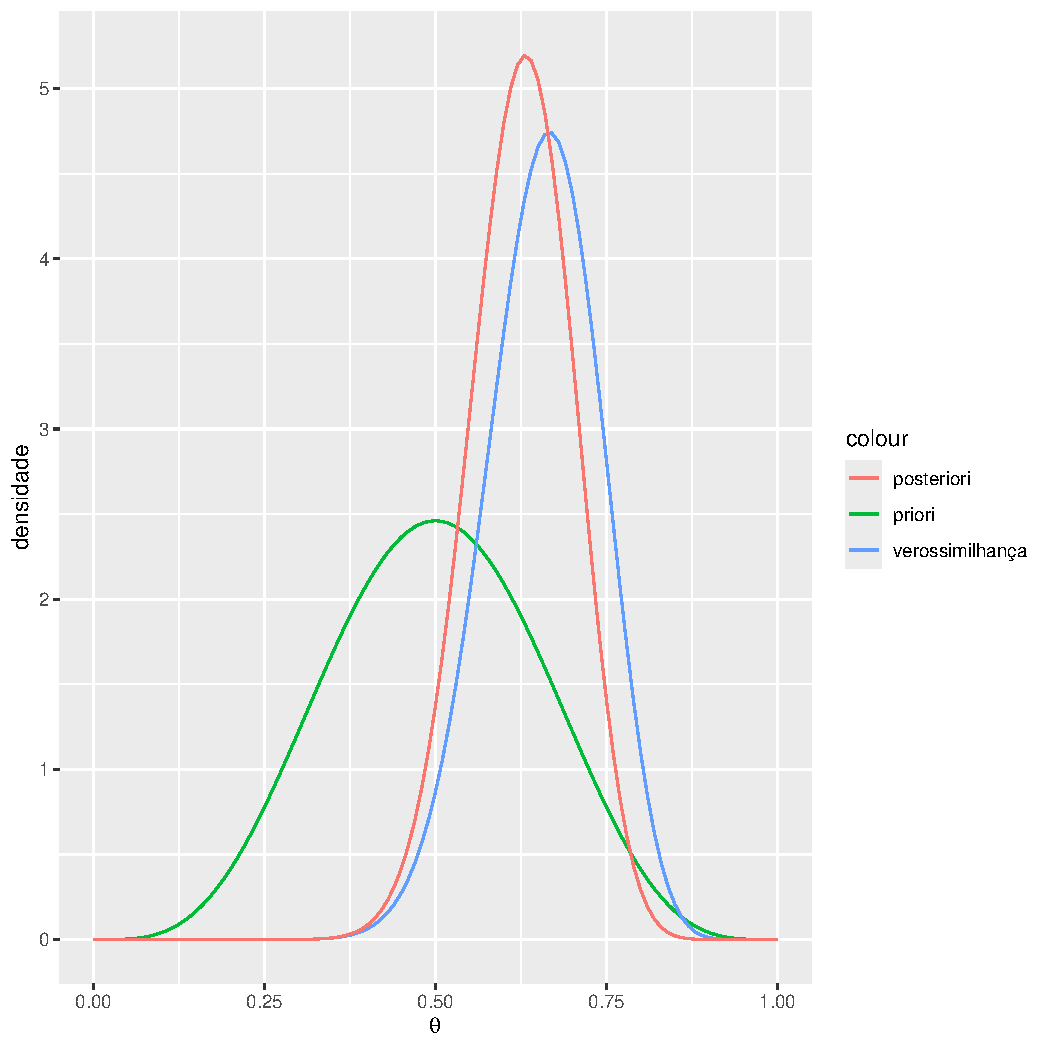
\includegraphics[width=\maxwidth]{./figures/unnamed-chunk-5-1} 
\end{knitrout}
 \caption{Comparação entre a distribuição a priori, a verossimilhança, e a distribuição a posteriori no \cref{exemplo:eleicao}.}
 \label{figura:eleicao}
\end{figure}

\end{example}

\subsubsection*{Exercícios}

\begin{exercise}
 No \cref{exemplo:exame}, qual é a 
 probabilidade de o exame indicar que não há câncer? 
 (antes de saber o resultado do exame)
\end{exercise}

\solution{
 \textbf{Solução}:
 \begin{align*}
  \P(E)	
  &= \P(E \cap C) + \P(E \cap C^{c})
  &	\Cref{ltp} \\
  &= \P(C)\P(E|C) + \P(C^{c})\P(E|C^{c}) \\
  &= 0.05 \cdot 0.8 + 0.95 \cdot 0.1 \\
  &= 0.135
 \end{align*}
 Portanto, conclua do 
 \cref{lemma:complement_probability} que
 $\P(E^{c}) = 1-\P(E) = 0.865$.
}{}

\begin{exercise}
 Um homicídio foi cometido em uma cidade de
 aproximadamente $100.000$ habitantes adultos.
 Antes de observar as evidências do caso, 
 o juiz acreditava que qualquer um dos habitantes
 poderia ter cometido o crime com mesma probabilidade.
 Contudo, a promotoria traz um exame forense como
 evidência de que o réu cometeu o crime.
 Por um lado, caso o réu seja culpado, 
 os resultados do exame seriam 
 observados com certeza.
 Por outro lado, caso o réu fosse inocente, 
 os resultados do exame somente seriam 
 observados com uma probabilidade de 
 $1$ em $10.000$.
 O promotor alega que há
uma baixa probabilidade de que
o réu seja inocente, e que ele deve portanto ser condenado.
 O juiz contrata você como uma
 perita judicial para ajudá-lo a 
 entender o argumento do promotor.
 Qual é a sua análise?
 
 Ressalvadas algumas adaptações, 
 este argumento jurídico é real e
 foi apresentado nos Estados Unidos no
 caso \emph{The People v. Collins}.
\end{exercise}

\solution{
 \textbf{Solução}: Considere os seguintes eventos:
 \begin{itemize}
  \item $R$: o réu cometeu o crime.
  \item $E$: o exame forense indica que 
  o réu cometeu o crime.
 \end{itemize}
 O promotor indicou que 
 $\P(E|R^{c}) = 10^{-4}$ e $\P(E|R) = 1$ e
 disse que isso é razão suficiente para 
 acreditar que o réu é 
 culpado dada a evidência.
 Contudo, o juiz acreditava, a priori, que
 $\P(R) = 10^{-5}$.
 Para determinar a probabilidade a posteriori de que
 o réu é culpado, $\P(R|E)$, 
 ele deve usar o teorema de Bayes.
 \begin{align*}
  \P(R|E)
  &= \frac{\P(R)\P(E|R)}{\P(R)\P(E|R)
  +\P(R^{c})\P(E|R^{c})}
  & \text{\Cref{bayes}} \\
  &=\frac{10^{-5} \cdot 1}
  {10^{-5} \cdot 1 + (1-10^{-5}) \cdot 10^{-4}} \\
  &=\frac{10^{-5}}
  {10^{-5}+10^{-4}-10^{-9}}
  = \frac{1}{10+1-10^{-4}} \approx 11^{-1}
  \approx 0.091
 \end{align*}
 Portanto, dado o resultado do exame forense,
 a probabilidade de que o réu é culpado ainda é baixa.
 Isto ocorre dada a baixa probabilidade a priori de que
 o réu era culpado. O argumento falacioso usado pelo
 promotor é bem conhecido em Estatística Forense e
 recebe o nome de \href{https://en.wikipedia.org/wiki/Prosecutor\%27s_fallacy}{``falácia do promotor''}.
}{}

\begin{exercise}[Monty Hall]
 Marilyn vos Savant por muitos anos foi considerada
 a pessoa com o maior QI do mundo (228) pelo
 livro Guiness. Ela é a autora da coluna 
 ``Ask Marilyn'', em que responde a 
 perguntas de seus leitores.
 Em um episódio célebre,
 sua resposta a uma pergunta de probabilidade
 gerou polêmica na época.
 A pergunta era a seguinte:
 \begin{quote}
  Suponha que você está em um programa de televisão.
  O apresentador te permite escolher entre três portas.
  Atrás de uma das portas há uma carro e 
  atrás das outras duas há cabras.
  Você ganhará o carro caso abra a sua respectiva porta.
  Considere que, a priori, você acredita ser
  equiprovável que o carro está atrás de 
  cada uma das portas.
  Após você escolher a porta $1$, o apresentador sempre
  abrirá aleatoriamente (dentre as portas que
  você não escolheu) uma das portas com uma cabra e
  te dará a oportunidade de trocar de porta.
  Digamos que o apresentador abriu a porta $2$.
  É vantajoso trocar de porta?
 \end{quote}

 Marylin vos Savant respondeu que era vantajoso.
 Você concorda com ela?
\end{exercise}

\solution{
 \textbf{Solução}: Considere os seguintes eventos:
 \begin{itemize}
  \item $Pr_{i}$: O prêmio está atrás da porta $i$.
  \item $C_{2}$: O apresentador abrirá a porta $2$.
 \end{itemize}
 O problema indica que $\P(Pr_{i}) = 3^{-1}$.
 Note que se o prêmio está atrás da porta $1$, então
 o apresentador poderia abrir 
 tanto a porta $2$ quanto a $3$.
 Como ele toma uma decisão entre 
 as disponíveis com mesma probabilidade,
 $\P(C_{2}|Pr_{1}) = 2^{-1}$.
 Se o prêmio está atrás da porta $2$, então
 o apresentador certamente não a abrirá, 
 $\P(C_{2}|Pr_{2}) = 0$.
 Finalmente, se o prêmio está atrás da porta $3$,
 então o apresentador não pode abrir a porta que
 você escolheu ($1$),
 nem a porta que tem o prêmio ($3$) e, assim,
 deve abrir a porta $2$, $\P(C_{2}|Pr_{3}) = 1$.
 Finalmente, podemos usar o 
 Teorema de Bayes para achar $\P(Pr_{1}|C_{2})$.
 \begin{align*}
  \P(Pr_{1}|C_{2})	
  &= \frac{\P(Pr_{1})\P(C_{2}|Pr_{1})}
  {\P(Pr_{1})\P(C_{2}|Pr_{1}) 
  +\P(Pr_{2})P(C_{2}|Pr_{2}) 
  +\P(Pr_{3})P(C_{2}|Pr_{3})}
  & \Cref{bayes} \\
  &= \frac{3^{-1} \cdot 2^{-1}}{3^{-1} \cdot 2^{-1}
  +3^{-1} \cdot 0 + 3^{-1} \cdot 1} \\
  &= \frac{1}{1 + 2} = 3^{-1}
 \end{align*}
 Realizando as mesmas contas para 
 as outras portas, obtemos 
 $\P(Pr_{2}|C_{2}) = 0$ e 
 $\P(Pr_{3}|C_{2}) = 2 \cdot 3^{-1}$.
 Portanto, dado que a posteriori a porta $3$ é 
 mais provável que a $1$,
 vale a pena trocar de porta.
}{}

\begin{exercise}
 Sejam $A_{1},\ldots,A_{n}$ eventos disjuntos tais que
 $\Omega = \cup_{i=1}^{n}{A_{i}}$.
 Prove que 
 \begin{align*}
  \P(A_{1}|B)
  &= \frac{\P(A_{1})\P(B|A_{1})}
  {\sum_{i=1}^{n}{\P(A_{i})\P(B|A_{i})}}
 \end{align*}
\end{exercise}

\solution{
 \textbf{Solução}:
 \begin{align*}
  \P(A_{1}|B)
  &= \frac{\P(A_{1} \cap B)}{\P(B)}
  & \text{\Cref{conditional_probability}} \\
  &= \frac{\P(A_{1})\P(B|A_{1})}{\P(B)}
  & \text{\Cref{conditional_probability}} \\
  &= \frac{\P(A_{1})\P(B|A_{1})}
  {\P(B \cap (\cup_{i=1}^{n}{A_{i}}))}	
  & B = \cup_{i=1}^{n}{A_{i}} \\
  &= \frac{\P(A_{1})\P(B|A_{1})}
  {\P(\cup_{i=1}^{n}(B \cap {A_{i}}))} \\
  &= \frac{\P(A_{1})\P(B|A_{1})}
  {\sum_{i=1}^{n}\P(B \cap {A_{i}})}
  &	\text{\Cref{probability}} \\
  &= \frac{\P(A_{1})\P(B|A_{1})}
  {\sum_{i=1}^{n}\P(A_{i})\P(B|{A_{i}})}
  & \text{\Cref{conditional_probability}}
 \end{align*}
}{}

\subsection{Modelo estatístico}
\label{section:stat_model}

O modelo estatístico oferece uma 
tradução padronizada de problemas envolvendo incerteza
para um espaço de probabilidade.
Ele é suficientemente geral para que 
muitos problemas que envolvem incerteza possam 
ser traduzidos por meio dele.

Simplificadamente, os elementos do modelo estatístico são
os dados, denotados por $X$ (que pertencem ao espaço amostral $\mathcal{X}$), e 
uma quantidade desconhecida de interesse, denotada por
$\theta$. $\theta$ é comumente chamado de 
parâmetro do modelo.
Assumimos que $\theta \in \Theta$ ($\Theta$ é chamado de espaço paramétrico).
Nosso interesse é em fazer inferência (isto é, fazer afirmações) sobre $\theta$ após observar os dados $X=x$.


A essência da abordagem Bayesiana
para a inferência estatística
é tratar tanto $X$ quanto $\theta$ como
quantidades aleatórias. 
Isso é feito pois,  antes de observar $X$, ambas são
desconhecidas
e portanto temos incerteza sobre elas.

Veremos agora como essa perspectiva permite fazer  inferência sobre $\theta$.
Como $\theta$ e $X$
são aleatórios,
eles possuem uma função de
probabilidade 
conjunta.
Na prática Bayesiana, esta probabilidade conjunta é especificada
por dois elementos:
(i) a
probabilidade marginal de $\theta$,
denotada por $f(\theta_{0})$ 
(a distribuição \emph{a priori} dos parâmetros, que codifica matematicamente informações anteriores à realização do experimento) e (ii)
a
probabilidade dos dados condicional a $\theta$, denotada por $f(x|\theta_{0})$ (a função de verossimilhança, que codifica a informação sobre $\theta$ presente nos dados).\footnote{Note que o modelo Bayesiano está
especificando
uma função de
probabilidade (ou densidade) conjunta para 
$\theta$ e $X$, $f(x,\theta_{0})$. Em particular, $f(\theta_{0}) := \int{f(x,\theta_{0})dx}$. Ainda que essa distribuição é usualmente especificada como \emph{priori}+verossimilhança, ela poderia ser feita de outras maneiras.}
Estes dois elementos podem ser combinados através do Teorema de Bayes
de modo a se obter  $f(\theta_{0}|x)$, que é chamada de distribuição 
\emph{a posteriori} de $\theta$ e que codifica  a incerteza sobre $\theta$ após a realização do experimento: 
\begin{align}
 \label{eqn:bayes}
 f(\theta_{0}|x)
 &= \frac{f(\theta_{0})f(x|\theta_{0})}
 {\int_{\Theta}{f(\theta)f(x|\theta)d\theta}}.
\end{align}
Assim, o Teorema de Bayes é a ferramenta matemática que permite combinar  informações anteriores à realização do experimento
com os dados obtidos, de modo a se atualizar a incerteza sobre $\theta$ após se observar $x$.
A distribuição \emph{a posteriori} $f(\theta_{0}|x)$
contém toda a incerteza que temos
sobre $\theta$ após a realização do experimento.

Observe que $f(\theta_{0}|x)$ é 
uma função de $\theta_{0}$.
Também, $\int_{\Theta}{f(\theta)f(x|\theta)d\theta}$ 
não depende de $\theta_{0}$ ou, em outras palavras, 
esta integral é a constante que faz com que
$f(\theta_{0}|x)$ integre $1$.
Em alguns casos, é possível determinar a 
distribuição de $\theta|X$ sem 
calcular diretamente o valor da constante 
$\int_{\Theta}{f(\theta)f(x|\theta)d\theta}$.
Nestes casos, a seguinte notação é útil,
\begin{definition}
 \label{prop}
 Dizemos que $f(y) \propto g(y)$
 se existe alguma constante, $C \in \mathbb{R}$, 
 tal que $f(y) = C g(y)$.
\end{definition} 

\begin{lemma}
 \label{lemma:bayes_prop}
 \begin{align*}
  f(\theta_{0}|x)
  &\propto f(\theta_{0})f(x|\theta_{0})
 \end{align*}
 Note que $f(\theta_{0}|x)$ é uma função de 
 $\theta_{0}$ e que $x$ é uma constante.
 Isto ocorre pois, no paradigma Bayesiano,
 os dados, $x$, são conhecidos e a incerteza existe 
 a respeito de $\theta$.
 Por isso, $f(x) = \int{f(\theta)f(x|\theta)d\theta}$ 
 é uma constante.
 O ``$\theta$'' que aparece na integral é 
 uma variável de integração.
\end{lemma}

\begin{example}[``é proporcional a'' no
 \cref{exemplo:eleicao}]
 \begin{align*}
  f(\theta_{0}|x)
  &\propto f(\theta_{0})f(x|\theta_{0})
  & \text{\Cref{lemma:bayes_prop}} \\
  &=\beta^{-1}(5,5)\theta_{0}^{4}(1-\theta_{0})^{4} \cdot {30 \choose 20}\theta_{0}^{20}(1-\theta_{0})^{10}\I(\theta_{0})_{(0,1)} \\
  &\propto \theta_{0}^{24}(1-\theta_{0})^{14}I(\theta_{0})_{(0,1)}
 \end{align*}
 Observe que $\theta_{0}^{24}(1-\theta_{0})^{14}I(\theta_{0})_{(0,1)}$ é
 a forma funcional de uma distribuição Beta$(25,15)$.
 Portanto, a única constante que faz com que
 essa expressão integre $1$
 é $\beta^{-1}(25,15)$.
\end{example}

É comum que os dados sejam um vetor de 
valores observados, $X=(X_{1},\ldots,X_{n})$.
Ademais, é comum supor-se que
os elementos deste vetor sejam independentes e
identicamente distribuídos quando $\theta$ é conhecido.
Neste caso, podemos escrever
\begin{align*}
 f(x|\theta)
 &= \prod_{i=1}^{n}{f(x_{i}|\theta)}
\end{align*}
onde $f(x_{i}|\theta)$ é a distribuição marginal de
cada elemento do vetor $x$. Neste caso, obtemos,
\begin{lemma}
 \label{lemma:bayes_iid}
 Quando os dados são i.i.d. dado $\theta$, obtemos:
 \begin{align*}
  f(\theta_{0}|x)
  &= \frac{f(\theta_{0})\prod_{i=1}^{n}{f(x_{i}|\theta)}}
  {\int_{\Theta}{f(\theta)\prod_{i=1}^{n}
  {f(x_{i}|\theta)}d\theta}} \\
  &\propto f(\theta_{0})\prod_{i=1}^{n}
  {f(x_{i}|\theta)}
 \end{align*}
\end{lemma}

\subsubsection*{Exercícios}

\begin{exercise}
 Considere que, a priori, 
 $\theta \sim \text{Gamma}(2,2)$.
 Também, $X|\theta \sim \text{Poisson}(\theta)$.
 Qual é a distribuição a posteriori para 
 $\theta$ após observar que $X=2$?
  Use um software computacional para traçar (i) a  distribuição à priori, (ii) a função de verossimilhança e (iii) a distribuição à posteriori
 em função de 
 $\theta \in \mathbb{R}^+$.
 Interprete o gráfico resultante.
\end{exercise}

\solution{
 \textbf{Solução}:
 \begin{align*}
  f(\theta_{0}|x)
  &\propto f(\theta_{0}) f(x|\theta_{0}) \\
  &\propto \theta_{0}\exp(-2\theta_{0})
  \exp(-\theta_{0}) \theta_{0}^{x} \\
  &= \theta_{0}^{x+1} \exp(-(2+1)\theta_{0}) \\
  &= \theta_{0}^{(x+2)-1} \exp(-(2+1)\theta_{0}) 
 \end{align*}
 Portanto, $\theta|X=2 \sim \text{Gamma}(4, 3)$.
}{}

\begin{exercise}
 \label{exercicio:urna_com_rep}
 Considere que uma urna tem $3$ bolas.
 Cada uma das bolas pode ser branca ou azul.
 Você deseja determinar o número de bolas azuis na urna.
 A priori, você acredita que 
 todos os valores em $\{0,1,2,3\}$ são 
 equiprováveis para o número de bolas azuis.
 Para aprender mais sobre esta quantidade, você 
 retira duas bolas com reposição da urna e 
 observa que as duas são azuis.
 Qual é o modelo estatístico neste problema?
 Use o \cref{lemma:bayes_iid} para 
 obter sua probabilidade a posteriori.
\end{exercise}

\solution{
 \textbf{Solução}: Considere as 
 seguintes variáveis aleatórias:
 \begin{itemize}
  \item $\theta$: O número de bolas azuis na urna.
  \item $X_{i}$: A cor da bola na amostra $i$, 
  $i \in \{1,2\}$. $X_{i}=1$ se 
  a bola foi azul e $X_{i}=0$, caso contrário.
 \end{itemize}
 Note que foi realizada uma 
 amostragem simples com reposição. Portanto,
 $\P(X_{i}=1|\theta=\theta_{0}) = 3^{-1}\theta_{0}$.
 Também, dado que a amostragem foi 
 realizada com reposição,
 os elementos de $X$ são independentes quando
 o valor de $\theta$ é conhecido.
 Portanto, podemos aplicar o \cref{lemma:bayes_iid}: 
 \begin{align*}
  \P(\theta=0|X_{1}=1, X_{2}=1) 
  &\propto \P(\theta=0)\P(X_{1}=1|\theta=0)
  \P(X_{2}=1|\theta=0) \\
  &= 4^{-1} \cdot 0 \cdot 0 = 0 \\
  \P(\theta=1|X_{1}=1, X_{2}=1) 
  &\propto \P(\theta=1)\P(X_{1}=1|\theta=1)
  \P(X_{2}=1|\theta=1) \\
  &= 4^{-1} \cdot 3^{-1} \cdot 3^{-1} 
  = 2^{-2}3^{-2} \\
  \P(\theta=2|X_{1}=1, X_{2}=1) 
  &\propto \P(\theta=2)P(X_{1}=1|\theta=2)
  \P(X_{2}=1|\theta=2) \\
  &= 4^{-1} \cdot 2 \cdot 3^{-1} \cdot 2 \cdot 3^{-1} 
  = 3^{-2} \\
  \P(\theta=3|X_{1}=1, X_{2}=1)
  &\propto \P(\theta=3)P(X_{1}=1|\theta=3)
  \P(X_{2}=1|\theta=3) \\
  &= 4^{-1} \cdot 1 \cdot 1 = 2^{-2}
 \end{align*}
 Note que
 \begin{align*}
  \P(\theta=0|X_{1}=1, X_{2}=1)
  +\P(\theta=1|X_{1}=1, X_{2}=1)
  +\P(\theta=2|X_{1}=1, X_{2}=1)
  +\P(\theta=3|X_{1}=1, X_{2}=1) = 1
 \end{align*}
 Portanto, dividindo cada um dos resultados acima 
 pela soma dos resultados encontrados,
 \begin{align*}
  \begin{cases}
   \P(\theta=0|X_{1}=1, X_{2}=1)
   &= \frac{0}{2^{-2}3^{-2} + 3^{-2}+2^{-2}} = 0 \\
   \P(\theta=1|X_{1}=1, X_{2}=1)
   &= \frac{2^{-2}3^{-2}}{2^{-2}3^{-2}+ 3^{-2}+ 2^{-2}}
   \approx 0.071 \\
   \P(\theta=2|X_{1}=1, X_{2}=1)
   &= \frac{3^{-2}}{2^{-2}3^{-2}+3^{-2}+2^{-2}}
   \approx 0.286 \\
   \P(\theta=3|X_{1}=1, X_{2}=1)
   &= \frac{2^{-2}}{2^{-2}3^{-2} + 3^{-2} + 2^{-2}}
   \approx 0.643
  \end{cases}
 \end{align*}
 Alternativamente, temos:
 \begin{align*}
  \P(\theta=\theta_{0}|X_{1}=1, X_{2}=1)
  &\propto \P(\theta=\theta_{0})
  \P(X_{1}=1|\theta=\theta_{0})
  \P(X_{2}=1|\theta=\theta_{0}) \\
  &= \frac{1}{4} \cdot 
  \left(\frac{\theta_{0}}{3}\right)^{2}
  = \frac{\theta_{0}^{2}}{36}
 \end{align*}
 Usando o fato de que 
 $\sum_{i=1}^{3}{P(\theta=i|X_{1}=1, X_{2}=1)} = 1$,
 obtemos:
 \begin{align*}
  \P(\theta=\theta_{0}|X_{1}=1, X_{2}=1)
  &= \frac{\frac{\theta_{0}^{2}}{36}}{\sum_{i=0}^{3}
  {\frac{i^{2}}{36}}} 
  =\frac{\theta_{0}^{2}}
  {\sum_{i=1}^{3}{i^{2}}}
 \end{align*}
}{}

\begin{exercise}
 \label{exercicio:urna_sem_rep}
 Considere a mesma situação descrita no
 \cref{exercicio:urna_com_rep}.
 Contudo, considere que a retirada da urna foi 
 feita \textbf{sem} reposição.
 Encontre a sua probabilidade a posteriori. 
 (Você não pode usar o \cref{lemma:bayes_iid}
 neste caso!)
\end{exercise}

\solution{
 \textbf{Solução}: Considere as 
 mesmas variáveis aleatórias definidas no
 \cref{exercicio:urna_com_rep}.
 Neste caso, $X_{1}$ e $X_{2}$ não são 
 independentes sabendo o valor o de $\theta$.
 Em particular, temos que:
 \begin{align*} 
  \P(X_{1}=1 \cap X_{2}=1|\theta=\theta_{0}) 
  &= \frac{\theta_{0}(\theta_{0}-1)}{6}
 \end{align*}
 Utilizando o \cref{lemma:bayes_prop}, obtemos:
 \begin{align*}
  \P(\theta=\theta_{0}|X_{1}=1, X_{2}=1)
  &\propto \frac{1}{4} 
  \cdot \frac{\theta_{0}(\theta_{0}-1)}{6} \\
  &\propto \theta_{0}(\theta_{0}-1)
 \end{align*}
 Como $\sum_{i=0}^{3}{P(\theta=i|X_{1}=1, X_{2}=1)}=1$,
 obtemos:
 \begin{align*}
  \P(\theta=\theta_{0}|X_{1}=1, X_{2}=1)
  &= \frac{\theta_{0}(\theta_{0}-1)}
  {\sum_{i=0}^{3}{i(i-1)}}
 \end{align*}
}{}

\begin{exercise}
 Considere que, a priori, a proporção de
 indivíduos com uma determinada doença em
 uma população é uma uniforme em $(0,1)$.
 $100$ indivíduos são selecionados com reposição e
 verifica-se que $30$ deles tem a doença.
 Qual é a probabilidade a posteriori para 
 a proporção de indivíduos com a doença?
\end{exercise}

\solution{\textbf{Solução}: Definimos
 \begin{align*}
  \begin{cases}
   \theta: \text{proporção de indivíduos com 
   a doença na população} \\
   X: \text{número de indivíduos na amostra que 
   tem a doença}
  \end{cases}
 \end{align*}
 Temos que $\theta \sim \text{Uniforme}(0,1)$ e 
 $X|\theta \sim \text{Binomial}(100,\theta)$.
 Portanto,
 \begin{align*}
  f(\theta|X=30)
  &\propto f(\theta)f(X=30|\theta) \\
  &= \I_{[0,1]}(\theta){100 \choose 30}
  \theta^{30} (1-\theta)^{70} \\
  &\propto \theta^{30}(1-\theta)^{70}\I_{[0,1]}(\theta)
 \end{align*}
 Portanto, concluímos pela 
 forma de $f(\theta|X=30)$ que 
 $\theta|X=30 \sim \text{Beta}(31,71)$.
}{}

\begin{exercise}
 \label{ex:introduction-normal}
 Considere que, a priori, $\sigma^{2}$ tem 
 distribuição uniforme em $\{1,2\}$.
 Se $X|\sigma^{2} \sim N(0,\sigma^{2})$, qual 
 a posteriori de $\sigma^{2}$ dado $X$?
 Exiba a posteriori exata, não é 
 o suficiente indicá-la até uma 
 constante de proporcionalidade.
 Use um software computacional para traçar o 
 valor de $\P(\sigma^{2}=1|X=x)$ em função de 
 $x \in \mathbb{R}$.
 Interprete o gráfico resultante.
\end{exercise}

\solution{\textbf{Solução}:
 \begin{align*}
  f(\sigma^{2}=1|X=x)
  &= \frac{f(\sigma^{2}=1)f(x|\sigma^{2}=1)}
  {f(\sigma^{2}=1)f(x|\sigma^{2}=1)
  +f(\sigma^{2}=2)f(x|\sigma^{2}=2)} \\
  &= \frac{2^{-1}(\sqrt{2\pi})^{-1}\exp(-\frac{x^{2}}{2})}{2^{-1}(\sqrt{2\pi})^{-1}\exp(-\frac{x^{2}}{2}) +2^{-1}(\sqrt{4\pi})^{-1}\exp(-\frac{x^{2}}{4})} \\
  &= \frac{\exp(-\frac{x^{2}}{2})}{\exp(-\frac{x^{2}}{2}) +\sqrt{2^{-1}}\exp(-\frac{x^{2}}{4})} \\
  &= \frac{1}{1+ \sqrt{2^{-1}}\exp(\frac{x^{2}}{4})}
 \end{align*}
 A \cref{fig:ex2} mostra que,
 quanto mais distante de $0$ for o dado observado,
 menor a probabilidade a posteriori de que
 $\sigma^{2}=1$.
 Observe que, quando $\sigma^{2}=1$, a 
 variância de $X$ é pequena.
 Assim, esperamos que os dados estejam 
 concentrados em torno de $0$.
 Similarmente, quando $\sigma^{2}=2$, 
 a variância de $X$ é maior. 
 Assim, esperamos que os dados estejam mais 
 dispersos ao redor de $0$.
 A posteriori se adequa a este 
 comportamento qualitativo, dando maior 
 probabilidade para $\sigma^{2}=1$ quando 
 observamos dados que seriam esperados 
 sob esta hipótese.
 \begin{figure}
  %gerado por chapter-introduction-normal-sigma.R
  \centering
  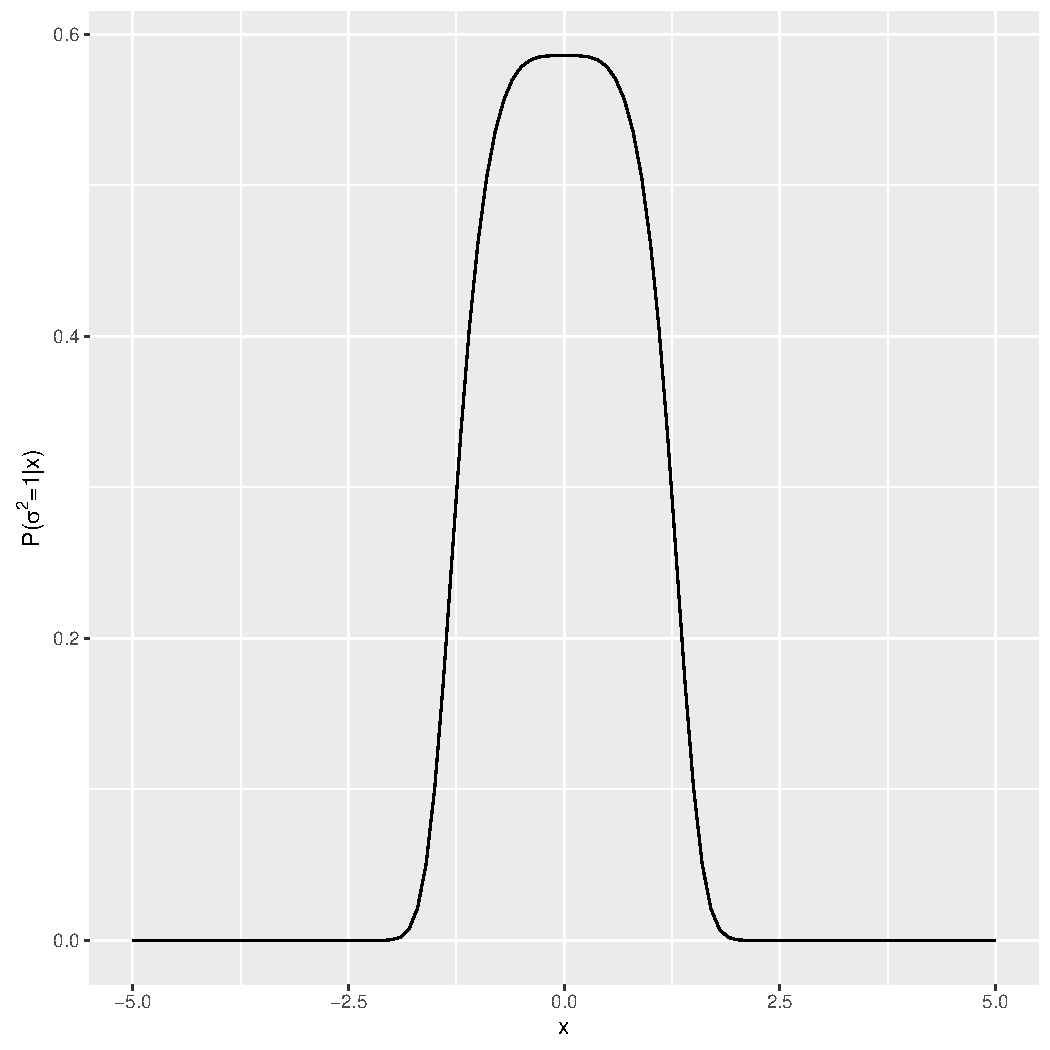
\includegraphics[scale=0.5]{chapter-introduction-normal.pdf}
  \caption{$P(\sigma^{2}=1|X=x)$ para o
  \cref{ex:introduction-normal}.}
  \label{fig:ex2}
 \end{figure}
}{}

\begin{exercise}
 O som inicial para uma palavra em 
 um idioma pode pertencer à categoria 
 consoante ou à categoria vogal. Considere que, 
 se o som inicial de um idioma é conhecido, 
 cada um dos seus descendentes terá o som inicial na
 mesma categoria do ancestral independentemente e 
 com probabilidade $0.9$.
 Considere que os idiomas $B$ e $C$ são 
 descendentes imediatos do idioma $A$.
 Contudo, não conhecemos os sons iniciais para 
 as palavras de $A$. Acreditamos que o som inicial para
 o sentido ``cachorro'' em $A$ é 
 uma consoante ou uma vogal com mesma probabilidade.
 Observamos que os sons iniciais dos
 idiomas $B$ e $C$ para ``cachorro'' são 
 ambos consoantes.
 Estamos interessados em predizer a 
 categoria do som inicial para 
 a palavra ``cachorro'' no idioma $A$.
 \begin{enumerate}[label=(\alph*)]
  \item Quais são os dados e 
  os parâmetros neste problema?
  \item Encontre a posteriori para o parâmetro.
  \item Qual seria a posteriori se 
  o som inicial para cada descendente estivesse 
  em uma categoria diferente?
 \end{enumerate}
\end{exercise}

\solution{\textbf{Solução}:
 \begin{enumerate}[label=(\alph*)]
  \item Defina $C$ como consoante e $V$ como vogal.
  Também,
  \begin{align*}
   \begin{cases}
    \theta: \text{a categoria do som inicial para 
    a palavra ``cachorro'' no idioma A},
    \theta \in \{C,V\}	\\
    X_{1}: \text{a categoria do som inicial para 
    a palavra ``cachorro'' no idioma B},
    X_{1} \in \{C,V\} \\
    X_{2}: \text{a categoria do som inicial para
    a palavra ``cachorro'' no idioma C},
    X_{2} \in \{C,V\}
   \end{cases}
  \end{align*}
  Seguindo a convenção usual, $\theta$ é o parâmetro,
  uma quantidade de interesse desconhecida, e 
  $X=(X_{1},X_{2})$ são os dados, 
  quantidades observáveis.
  
  \item
  \begin{align*}
   \P(\theta=C|X_{1}=C, X_{2}=C)
   &= \frac{\P(\theta=C)\P(X_{1}=C,X_{2}=C|\theta=C)}
   {\P(\theta=C)P(X_{1}=C,X_{2}=C|\theta=C)
   +\P(\theta=V)P(X_{1}=C,X_{2}=C|\theta=V)} \\
   &= \frac{0.5 \cdot 0.9 \cdot 0.9}
   {0.5 \cdot 0.9 \cdot 0.9 
   +0.5 \cdot 0.1 \cdot 0.1}\\
   &\approx 0.988
  \end{align*}
  Como $\P(\theta=C|X_{1}=C, X_{2}=C) + \P(\theta=V|X_{1}=C, X_{2}=C) = 1$, obtemos
  \begin{align*}
   \P(\theta=V|X_{1}=C, X_{2}=C) &= 0.012
  \end{align*}
  
  \item
  \begin{align*}
   \P(\theta=C|X_{1}=C, X_{2}=V)
   &= \frac{\P(\theta=C)\P(X_{1}=C,X_{2}=V|\theta=C)}
   {\P(\theta=C)\P(X_{1}=C,X_{2}=V|\theta=C)
   +\P(\theta=V)\P(X_{1}=C,X_{2}=V|\theta=V)} \\
   &= \frac{0.5 \cdot 0.9 \cdot 0.1}
   {0.5 \cdot 0.9 \cdot 0.1 
   +0.5 \cdot 0.1 \cdot 0.9} \\
   &= 0.5
  \end{align*}
  Como $\P(\theta=C|X_{1}=C, X_{2}=C) + \P(\theta=V|X_{1}=C, X_{2}=C) = 1$, obtemos
  \begin{align*}
   \P(\theta=V|X_{1}=C, X_{2}=C) = 0.5
  \end{align*}
 \end{enumerate}
}{}

\begin{exercise}
 Considere que um sistema é composto por $3$ peças e 
 que o sistema falha quando qualquer uma 
 das peças falhar.
 Considere que cada peça falha independentemente
 em um tempo (em dias) determinado pela 
 mesma taxa de falha.
 Assuma que, dada a taxa de falha, $\theta$,
 o tempo para falha de uma peça é uma
 Exponencial$(\theta)$.
 \begin{enumerate}[label=(\alph*)]
  \item Qual é a taxa de falha do sistema?
  \item Considere que, a priori, 
  você acreditava que a taxa de falha de 
  cada componente seguia uma distribuição Gamma$(1,1)$.
  Se você observou um sistema falhar em $3$ dias,
  qual é a sua posteriori para a taxa de falha dos
  componentes?
  Identifique o nome e os hiperparâmetros da
  distribuição a posteriori.
 \end{enumerate}
\end{exercise}

\solution{\textbf{Solução}:
 \begin{enumerate}[label=(\alph*)]
  \item Defina
  \begin{align*}
   \begin{cases}
    \theta: \text{a taxa de falha dos componentes}.	\\
    X_{i}: \text{o tempo até o componente $i$ falhar}.\\
	Y: \text{o tempo até o sistema falhar}.
   \end{cases}
  \end{align*}
  O problema indica que, dado $\theta$,
  $X_{1},X_{2}$ e $X_{3}$ são independentes e
  $X_{i} \sim \text{Exponencial}(\theta)$.
  Temos que
  \begin{align*}
   \P(Y \geq t|\theta)
   &= \P(X_{1} \geq t, X_{2} \geq t, X_{3} \geq t |\theta) \\
   &= \P(X_{1} \geq t|\theta)\P(X_{2} \geq t|\theta)\P(X_{3} \geq t|\theta) \\
   &= \exp(-t\theta)\exp(-t\theta)\exp(-t\theta) 
   =\exp(-t \cdot 3\theta)
  \end{align*}
  Portanto, $Y|\theta \sim \text{Exponencial}(3\theta)$.
  
  \item
  \begin{align*}
   f(\theta|Y=3)
   &\propto f(\theta)f(Y=y|\theta) \\
   &\propto \exp(-\theta)3\theta \exp(-9\theta) \\
   &\propto \theta^{2-1}\exp(-10\theta)
  \end{align*}
  Portanto $\theta|Y=3 \sim \text{Gamma}(2,10)$.
 \end{enumerate}
}{}

\begin{exercise}
 Dado $\theta$, $X_{1}, \ldots X_{n}$ são
 independentes. Mostre que 
 \begin{align*}
  f(\theta|x_{1},\ldots,x_{n}) 
  &\propto f(\theta|x_{1},\ldots,x_{n-1})
  f(x_{n}|\theta)
 \end{align*}
 Em outras palavras, a posteriori obtida após 
 condicionar nas observações anteriores pode ser 
 usada como priori na aplicação do Teorema de Bayes para
 a próxima observação.
\end{exercise}

\solution{\textbf{Solução}:
 \begin{align*}
  f(\theta|x_{1},\ldots,x_{n})
  &\propto f(\theta)f(x_{1},\ldots,x_{n}|\theta)
  &	\text{\cref{lemma:bayes_prop}} \\
  &= f(\theta)f(x_{1},\ldots,x_{n-1}|\theta)
  f(x_{n}|\theta)
  & \text{indep. dado $\theta$} \\
  &\propto f(\theta|x_{1},\ldots,x_{n-1})
  f(x_{n}|\theta)
  & \text{\cref{lemma:bayes_prop}}
 \end{align*}
}{}

\newpage

\section{Coerência e Probabilidade: 
como evitar prejuízos certos?}

\subsection{Probabilidade marginal}

Em cursos anteriores,
você usou a probabilidade como
uma forma de representar a sua incerteza.
Contudo, possivelmente você não viu o porquê
dessa representação ser razoável.
Por que é razoável assumir
que a representação da sua incerteza satisfaz
os axiomas da probabilidade (\cref{probability})?

\begin{enumerate}
 \item (Não-negatividade) Para todo $A$, 
 $\P(A) \geq 0$.
 \item (Aditividade) Se $(A_{n})_{n \in \mathbb{N}}$ é
 uma sequência de conjuntos disjuntos, então
 $\P(\cup_{n \in \mathbb{N}}{A_{n}}) = \sum_{n \in \mathbb{N}}{\P(A_{n})}$.
 \item (Normalização) $\P(\Omega) = 1$.
\end{enumerate}

Neste Capítulo, 
discutiremos a questão acima.
Para tal, faremos uso de um experimento mental.
Considere que $A$ é uma proposição 
sobre a qual você tem incerteza.
Por exemplo, $A$ pode designar o
evento de que choverá amanhã.
Também considere uma aposta tal que 
o vendedor deve pagar $R\$1$ ao comprador se $A$ ocorrer e
$R\$0$, caso contrário.
Qual seria o preço tal que você aceitaria
tanto comprar quanto vender esta aposta?
Chamaremos este preço de $\text{Pr}(A)$.

Note que $\text{Pr}$ é uma representação da sua incerteza.
Quanto maior o valor de $\text{Pr}(A)$,
mais você acredita que $A$ irá ocorrer.
Também, o seu valor de $\text{Pr}$ não necessariamente
é o mesmo de seus colegas, 
cada um podendo coerentemente ter os seus próprios preços.
Isto significa que você pode coerentemente designar
qualquer valor a $\text{Pr}(A)$?

Para responder a esta pergunta,
é necessário definir coerência.
Dizemos que uma designação de preços é
incoerente se ela é tal que você pode
perder dinheiro com certeza.
Observar que você está incorrendo em perda certa
provavelmente te daria incentivo suficiente
para rever seus preços e a incerteza
das proposições ligadas a estes.
Portanto, investigaremos sob quais condições 
você incorre em perda certa.

Para tal, faremos uso da \cref{indicator_function}.
Lembre-se que $\I_{A}$ é a função indicadora
da proposição $A$, 
uma variável aleatória que assume o valor
$1$, quando $A$ ocorre, e $0$, caso contrário.
Assim, o seu lucro após comprar a aposta em $A$
pode ser escrito como $\I_{A}-\text{Pr}(A)$.
O resultado desta variável aleatória é resumido
na Tabela \ref{table:aposta_comprar}.
Note que, se $\text{Pr}(A) > 1$,
então o seu ganho obtido é sempre menor do que $0$.
Em outras palavras, você está tendo prejuízo certo.
Assim, para que $\text{Pr}(A)$ 
seja uma representação coerente da sua incerteza,
é necessário que $\text{Pr}(A) \leq 1$.

\begin{table}
 \centering
 \begin{tabular}{|l|l|}
  \hline
  & $\I_{A}-\text{Pr}(A)$ \\
  \hline
  $A$ ocorre & $1-\text{Pr}(A)$ \\
  $A$ não ocorre & $-\text{Pr}(A)$ \\
  \hline
 \end{tabular}
 \caption{Ganho obtido comprando uma aposta em $A$.}
 \label{table:aposta_comprar}
\end{table}

Similarmente, podemos considerar o caso em que 
você vende a aposta em $A$.
Neste caso, o seu lucro é dado por 
$-(I_{A}-\text{Pr}(A))$.
Esta variável é resumida na \cref{table:aposta_vender}.
Observe que, se $\text{Pr}(A) < 0$, 
então $-(\I_{A}-\text{Pr}(A))$ é sempre menor que $0$.
Novamente, este caso te levaria a um prejuízo certo.
Portanto, também podemos concluir que,
se $\text{Pr}$ representa coerentemente a sua incerteza,
então $\text{Pr}(A) \geq 0$.
As considerações apresentadas acima 
nos levam ao resultado no \cref{lemma:sure_loss_1}.

\begin{table}
 \centering
 \begin{tabular}{|l|l|}
 \hline
  & $-(\I_{A}-\text{Pr}(A))$ \\
  \hline
  $A$ ocorre & $\text{Pr}(A)-1$ \\
  $A$ não ocorre & $\text{Pr}(A)$ \\
  \hline
 \end{tabular}
 \caption{Ganho obtido vendendo uma aposta em $A$.}
 \label{table:aposta_vender}
\end{table}

\begin{lemma}
 \label{lemma:sure_loss_1}
 Se existe $A$ tal que $\text{Pr}(A) < 0$ ou
 $\text{Pr}(A) > 1$, então 
 você pode ser levada a prejuízo certo.
\end{lemma}

Para prosseguir na análise,
consideraremos a composição de apostas.
Em outras palavras, avaliaremos o resultado
de você compor apostas, comprando e 
vendendo apostas em eventos individuais.
Formalmente, para quaisquer números,
$\alpha_{1}, \ldots, \alpha_{n}$,
e eventos, $A_{1}, \ldots, A_{n}$,
denotamos um portfólio de apostas por $(\alpha_{i},A_{i})_{1 \leq i \leq n}$.
Este portfólio é tal que,
se $\alpha_{i} > 0$, então você 
comprará $\alpha_{i}$ unidades da aposta em $A_{i}$ e,
se $\alpha_{i} < 0$, então você 
venderá $\alpha_{i}$ unidades desta aposta.
Note que o seu balanço dado pelo portfólio $(\alpha_{i},A_{i})_{1 \leq i \leq n}$ é 
$\sum_{i=1}^{n}{\alpha_{i}(\I_{A_{i}}-\text{Pr}(A_{i}))}$.
Em outras palavras, $\sum_{i=1}^{n}{\alpha_{i}(\I_{A_{i}}-\text{Pr}(A_{i}))}$ é 
a soma do resultado de todas as apostas 
em que você participou.

\begin{definition}
 Você pode ser levada a prejuízo certo se 
 existe um portfólio de apostas,
 $(\alpha_{i},A_{i})_{1 \leq i \leq n}$,
 tal que você perde dinheiro com certeza. 
 Isto é, para todo $\omega \in \Omega$,
 $\sum_{i=1}^{n}{\alpha_{i}(\I_{A_{i}}(w)-\text{Pr}(A_{i}))} < 0$.
\end{definition}

O próximo lema será uma ferramenta importante
para provar que certas atribuições de preços
levam a prejuízo certo.
Ele mostra que, como você está disposta tanto
a comprar quanto a vender quaisquer apostas,
então um portfólio com balanço constante e
diferente de $0$ a levará a prejuízo certo.

\begin{lemma}
 \label{lemma:constant_balance}
 Considere que para todo $\omega \in \Omega$,
 $\sum_{i=1}^{n}{\alpha_{i}(\I_{A_{i}(w)}-\text{Pr}(A_{i}))}$
 assume um valor constante, $c$.
 Se $c \neq 0$, então você pode ser levada 
 a prejuízo certo.
\end{lemma}

\begin{proof}
 Se $c < 0$, então o portfólio
 $(\alpha_{i},A_{i})_{1 \leq i \leq n}$
 traz um balanço $c$ e a leva a prejuízo certo.
 Se $c > 0$, então note que 
 o balanço do portfólio 
 $(-\alpha_{i},A_{i})_{1 \leq i \leq n}$ é:
 \begin{align*}
  &\sum_{i=1}^{n}{-\alpha_{i}(\I_{A_{i}(w)}-\text{Pr}(A_{i}))} \\
  =&-\sum_{i=1}^{n}{\alpha_{i}(\I_{A_{i}(w)}-\text{Pr}(A_{i}))} = -c
 \end{align*}
 Portanto, existe um portfólio, 
 $(-\alpha_{i},A_{i})_{1 \leq i \leq n}$,
 que a leva a prejuízo certo.
\end{proof}

O \cref{lemma:constant_balance} nos permite provar
mais resultados a respeito da 
atribuição coerente de preços.

\begin{lemma}
 \label{lemma:sure_loss_2}
 Se $\text{Pr}(\Omega) \neq 1$,
 então você pode ser levada a prejuízo certo.
\end{lemma}

\begin{proof}
 Note que o balanço da compra de 
 uma unidade de $\Omega$, 
 $((1,\Omega))$, é dado por 
 $\I_{\Omega}-\text{Pr}(\Omega)$.
 Também, $\I_{\Omega}$ é outra forma de escrever $1$.
 Assim, o balanço de $((1,\Omega))$ é
 $1-\text{Pr}(\Omega)$, uma constante.
 Portanto, o \cref{lemma:constant_balance} garante que,
 se $1-\text{Pr}(\Omega) \neq 0$,
 então seus preços a levam a prejuízo certo.
 Em outras palavras, para evitar prejuízo certo
 é necessário que $\text{Pr}(\Omega) = 1$.
\end{proof}

\begin{lemma}
 \label{lemma:sure_loss_3}
 Se existem $A$ e $B$ disjuntos tais que
 \begin{align*}
  \text{Pr}(A \cup B) \neq \text{Pr}(A)+\text{Pr}(B)
 \end{align*}
 então você pode ser levada a prejuízo certo.
\end{lemma}

\begin{proof}
 Como $A$ e $B$ são disjuntos, 
 existem três possíveis ocorrências:
 $A$, $B$ ou $(A \cup B)^{c}$ 
 (como $A$ e $B$ são disjuntos, $A \cap B$ é impossível).
 Portanto, o balanço de comprar $A$, 
 comprar $B$ e vender $A \cup B$ é 
 resumido pela \cref{table:aposta_uniao}.
 Note que o balanço do portfólio
 $((1,A),(1,B),(-1,A \cup B))$ é 
 constante e igual a 
 $\text{Pr}(A \cup B)-\text{Pr}(A)-\text{Pr}(B)$.
 Portanto, pelo \cref{lemma:constant_balance}, se
 $\text{Pr}(A \cup B)-\text{Pr}(A)-\text{Pr}(B) \neq 0$,
 você pode ser levada a prejuízo certo.
\end{proof}

\begin{table}
 \centering
 \begin{tabular}{|l|l|l|l|l|}
  \hline
  & $\I_{A}(w)-\text{Pr}(A)$
  & $\I_{B}(w)-\text{Pr}(B)$
  & $-(\I_{(A \cup B)}-\text{Pr}(A \cup B))$
  & portfólio (soma) \\
  \hline
  $\omega \in A$
  & $1-\text{Pr}(A)$
  & $-\text{Pr}(B)$
  & $\text{Pr}(A \cup B)-1$
  &	$\text{Pr}(A \cup B)-\text{Pr}(A)-\text{Pr}(B)$ \\
  $\omega \in B$ 
  & $-\text{Pr}(A)$
  & $1-\text{Pr}(B)$
  &	$\text{Pr}(A \cup B)-1$
  &	$\text{Pr}(A \cup B)-\text{Pr}(A)-\text{Pr}(B)$ \\
  $\omega \in (A \cup B)^{c}$
  & $-\text{Pr}(A)$
  & $-\text{Pr}(B)$
  & $\text{Pr}(A \cup B)$
  & $\text{Pr}(A \cup B)-\text{Pr}(A)-\text{Pr}(B)$ \\
  \hline
 \end{tabular}
 \caption{Ganho obtido por um portfólio que 
 compra $A$, compra $B$ e vende $A \cup B$, 
 quando $A$ e $B$ são disjuntos.}
 \label{table:aposta_uniao}
\end{table}

Resumindo os \cref{lemma:sure_loss_1,lemma:sure_loss_2,lemma:sure_loss_3},
obtemos condições que $\text{Pr}$ necessariamente deve obedecer para que você não possa ser levada
a prejuízo certo.

\begin{lemma}
 \label{lemma:sure_loss_additivity}
 Se $\text{Pr}$ é tal que 
 você não pode ser levada a prejuízo certo, então 
 é necessário que:
 \begin{enumerate}
  \item (Não-negatividade) Para todo $A$, 
  $0 \leq \text{Pr}(A) \leq 1$.
  \item (Aditividade) Se $A$ e $B$ são disjuntos, então
  $\text{Pr}(A \cup B) = \text{Pr}(A)+\text{Pr}(B)$.
  \item (Normalização) $\text{Pr}(\Omega) = 1$.
 \end{enumerate}
\end{lemma}

\begin{proof}
 Decorre dos \cref{lemma:sure_loss_1,lemma:sure_loss_2,lemma:sure_loss_3}.
\end{proof}

\subsubsection*{Exercícios}

\begin{exercise}[{\citet[p.8]{Kadane2011}}]
 Considere os seguintes eventos:
 \begin{itemize}
  \item $A_{1}$: Choverá amanhã e 
  a temperatura máxima será superior a $25^o$ C.
  \item $A_{2}$: Choverá amanhã e 
  a temperatura máxima não será superior a $25^o$ C.
  \item $A_{3}$: Não choverá amanhã e 
  a temperatura máxima será superior a $25^o$ C.
  \item $A_{4}$: Não choverá amanhã e 
  a temperatura máxima não será superior a $25^o$ C.
 \end{itemize}
 Quais seriam os preços que 
 você definiria para cada proposição e
 qual a sua linha de raciocínio?
 Os seus preços são coerentes?
 Se não, você estaria disposta a revê-los?
\end{exercise}

\solution{
 \textbf{Solução}: Este exercício visa enfatizar que
 a probabilidade é subjetiva e, assim, 
 é possível que diversas pessoas tenham
 probabilidades diferentes, todas elas sendo coerentes.
 Contudo, note que algumas probabilidades tem 
 maior poder de convencimento do que outras.
 Uma pessoa que meramente indica preços coerentes,
 sem dar justificativas por trás deles, 
 dificilmente convencerá seus colegas.
 Por outro lado, neste exercício,
 preços baseados em conhecimento climático e 
 histórico da região provavelmente terão 
 maior poder de convencimento.
}{}

\begin{exercise}
 Mostre que se $\text{Pr}(\emptyset) \neq 0$,
 então você pode ser levada a prejuízo certo.
\end{exercise}

\solution{
 \textbf{Solução}: Considere a compra de 
 uma aposta em $\emptyset$.
 O balanço desta aposta é dado por 
 $\I_{\emptyset}-\text{Pr}(\emptyset)$.
 Como $\emptyset$ nunca ocorre, 
 $\I_{\emptyset}=0$ e 
 o balanço da aposta é simplesmente 
 $-\text{Pr}(\emptyset)$.
 Portanto, esta aposta tem balanço constante.
 Conclua pelo \cref{lemma:constant_balance} que,
 se $\text{Pr}(\emptyset) \neq 0$,
 então você pode ser levada a prejuízo certo.
}{}

\begin{exercise}
 Se o prêmio das apostas fosse modificado de 
 $R\$1,00$ para $R\$2,00$, 
 alguma das condições para 
 a coerência de preços seria modificada?
 De que forma a sua resposta afeta a 
 sua interpretação do quanto é razoável 
 a analogia de apostas?
\end{exercise}

\solution{
 \textbf{Solução}: Se o prêmio ganho nas apostas 
 fosse modificado para $R\$2,00$,
 então o balanço de uma aposta $(\alpha_{i},A_{i})$ seria
 dado por $\alpha_{i}(2\I_{A_{i}}-\text{Pr}(A_{i}))$.
 Acompanhando os mesmos portfólios utilizados
 nos \cref{lemma:sure_loss_1,lemma:sure_loss_2,lemma:sure_loss_3},
 obtem-se que são condições necessárias para 
 evitar perda certa que:
 \begin{enumerate}
  \item para todo $A$, 
  $0 \leq \text{Pr}(A) \leq 2$.
  \item $\text{Pr}(\Omega) = 2$.
  \item Se $A$ e $B$ são disjuntos, então
  $\text{Pr}(A \cup B) = \text{Pr}(A)+\text{Pr}(B)$.
 \end{enumerate}
 Note que $\frac{\text{Pr}}{2}$ satisfaz 
 todos os axiomas da probabilidade.
 Mais especificamente, $\text{Pr}$ ainda pode 
 ser visto como uma representação de sua incerteza,
 dado que, quanto maior sua confiança em $A$, 
 mais estaria disposta a pagar para obter 
 $\alpha_{i}(2\I_{A_{i}}-\text{Pr}(A_{i}))$.
 Neste sentido, o prêmio de $R\$1,00$ é 
 uma condição que faz com que $\text{Pr}(\Omega)=1$ e,
 assim, normaliza os preços obtidos.
}{}

\begin{exercise}
 Mostre que, se 
 $Pr(A \cup B) \neq Pr(A) + Pr(B) - Pr(A \cap B)$,
 então você pode ser levada a prejuízo certo.
\end{exercise}

\subsection{Probabilidade condicional}

Na seção passada, 
discutimos uma analogia entre
os axiomas da probabilidade e apostas.
Contudo, esta analogia não nos permite obter
o axioma da probabilidade condicional.
Em outras palavras, o sistema de apostas
que estudamos não permite estudar de que
forma a incerteza é alterada com o aprendizado
de novos fatos.
Nesta seção, discutiremos uma extensão
da analogia de apostas que permite obter
o axioma da probabilidade condicional na \cref{conditional_probability}.

\begin{enumerate}
 \item $\P(A \cap B) = \P(B)\P(A|B)$
\end{enumerate}

Que tipo de aposta seria avaliada de acordo
com a sua incerteza em $A$ dado que $B$ ocorreu?
Para responder a essa pergunta,
é importante considerar qual o resultado da aposta
quando $B$ não acontece.
Uma saída é dizer que o comprador (e o vendedor)
tem um balanço de $0$ quando $B$ não acontece.
Assim, a aposta somente tem 
efeito sobre os apostadores quando $B$ ocorre.
Finalmente, para completar a aposta, quando $B$ ocorre,
consideramos uma aposta em que o comprador ganha 
$R\$1$ quando $A$ acontece e 
$R\$0$ quando $A$ não acontece.
Dizemos que a aposta definida acima é de 
$A$ condicional a $B$
e o seu preço para comprá-la é $\text{Pr}(A|B)$.
Observe que a aposta de $A$ condicional a $B$ é similar
à aposta da seção passada,
com a exceção de que ela só surte efeitos quando 
$B$ ocorre.
O balanço de comprar esta aposta pode ser resumido por $\I_{A \cap B} - \text{Pr}(A|B)\I_{B}$.
A \cref{table:aposta_a|b} ilustra este balanço.

\begin{table}
 \centering
 \begin{tabular}{|c|c|}
  \hline
  & $\I_{A \cap B} - \text{Pr}(A|B)\I_{B}$ \\
  \hline
  $A$ ocorre e $B$ ocorre
  & $1-\text{Pr}(A|B)$ \\
  $A$ não ocorre e $B$ ocorre
  & $-\text{Pr}(A|B)$ \\
  $B$ não ocorre
  & $0$ \\
  \hline
 \end{tabular}
 \caption{Balanço da compra da aposta de 
 $A$ condicional a $B$.} 
 \label{table:aposta_a|b}
\end{table}

Para obter um resultado a partir da aposta condicional,
também generalizaremos a definição anterior de 
portfólio de apostas.
Um portfólio de apostas será definido
como $(\alpha_{i},A_{i},B_{i})_{1 \leq i \leq n}$, 
onde $\alpha_{i}$ são números reais e
$A_{i}$ e $B_{i}$ são eventos.
Ao contrário da seção anterior, 
cada aposta em um portfólio é definida a partir 
de dois eventos.
Isto ocorre pois estamos comprando apostas de 
$A_{i}$ condicional a $B_{i}$.
Também é permitido que $\alpha_{i}$ seja 
qualquer número real.
A interpretação é similar ao caso anterior.
Por exemplo, se $\alpha_{i}=0.5$, compra-se 
$0.5$ unidade de uma aposta de
$A_{i}$ condicional a $B_{i}$.
Similarmente, se $\alpha_{i}=-0.37$, vende-se 
$0.37$ de uma unidade de uma aposta de 
$A_{i}$ condicional a $B_{i}$.
O balanço de um portfólio é dado pela
soma das apostas individuais,
isto é, ele é igual a $\sum_{i=1}^{n}{\alpha_{i}\left(\I_{A_i \cap B_i}-\text{Pr}(A_{i}|B_{i})\I_{B_i}\right)}$.

Antes de prosseguirmos, note que 
uma aposta de $A$ condicional a $\Omega$
tem exatamente o mesmo balanço que uma aposta em $A$.
Este é o caso pois $\Omega$ sempre ocorre.
Desta forma, para toda proposição $A$, definimos que 
$\text{Pr}(A) := \text{Pr}(A|\Omega)$.
Com essa definição, poderemos mostrar que 
$\text{Pr}(A \cap B) = \text{Pr}(B)\text{Pr}(A|B)$ é 
uma condição necessária para que 
você não possa ser levada a uma perda certa.

\begin{table}
 \centering
 \begin{tabular}{|c|c|c|c|}
  \hline
  & $(1,A,B)$
  & $(1, A^{c} \cap B, \Omega)$
  &	$(1-\text{Pr}(A|B),B^{c},\Omega)$ \\
  \hline
  $A$ ocorre e $B$ ocorre
  & $1-\text{Pr}(A|B)$
  &	$-\text{Pr}(A^{c} \cap B)$
  & $-(1-\text{Pr}(A|B))\text{Pr}(B^{c})$ \\
  $A$ não ocorre e $B$ ocorre
  & $-\text{Pr}(A|B)$
  & $1-\text{Pr}(A^{c} \cap B)$
  & $-(1-\text{Pr}(A|B))\text{Pr}(B^{c})$ \\
  $B$ não ocorre
  &	$0$
  & $-\text{Pr}(A^{c} \cap B)$
  & $(1-\text{Pr}(A|B))(1-\text{Pr}(B^{c}))$ \\
  \hline
 \end{tabular}
 \caption{Balanço da compra de 
 diversas apostas condicionais.} 
 \label{table:portfolio_a|b}
\end{table}

Para tal, considere um portfólio que 
consiste em comprar uma unidade de $A$ condicional a $B$,
comprar uma unidade de $B^{c}$ (condicional a $\Omega$) e 
comprar $(1+\text{Pr}(A|B))$ unidades de 
$A^{c} \cap B$ (condicional a $\Omega$).
A \cref{table:portfolio_a|b} resume os balanços para 
cada uma destas apostas.
Somando as colunas em cada uma das linhas, 
observamos que o balanço deste portfólio é 
constante e igual a
\begin{align*}
 1-\text{Pr}(A|B)-\text{Pr}(B^{c})
 -\text{Pr}(A^{c} \cap B)
 +\text{Pr}(A|B)\text{Pr}(B^{c})
\end{align*}
Utilizando o \cref{lemma:constant_balance}, observe que, como o portfólio tem balanço constante,
para que você possa evitar prejuízo certo é 
necessário que
\begin{align}
 \label{eqn:sure_loss_prob_condicional_1}
 0 = 1-\text{Pr}(A|B)-\text{Pr}(B^{c})
 -\text{Pr}(A^{c} \cap B)
 +\text{Pr}(A|B)\text{Pr}(B^{c})
\end{align}
Também, decorre do \cref{lemma:sure_loss_additivity} que,
para evitar prejuízo certo, é 
necessário que $\text{Pr}(B^{c}) = 1-\text{Pr}(B)$ e
$\text{Pr}(A^{c} \cap B) = \text{Pr}(B)-\text{Pr}(A \cap B)$. 
Realizando estas substituições na
\cref{eqn:sure_loss_prob_condicional_1},  obtemos:
\begin{align}
 \label{eqn:sure_loss_prob_condicional_2}
 0 &= 1-\text{Pr}(A|B)-(1-\text{Pr}(B))
 -(\text{Pr}(B)-\text{Pr}(A \cap B))
 +\text{Pr}(A|B)(1-\text{Pr}(B)) \nonumber \\
 0 &= \text{Pr}(A \cap B) 
 -\text{Pr}(B)\text{Pr}(A|B) \nonumber \\
 \text{Pr}(A \cap B) &= \text{Pr}(B)\text{Pr}(A|B)
\end{align}
Assim, para que você não possa ser 
levada a prejuízo certo,
é necessário que a 
\cref{eqn:sure_loss_prob_condicional_2} 
seja satisfeita.

\begin{lemma}
 \label{lemma:sure_loss_conditional}
 Se \text{Pr} é tal que você não pode 
 ser levada a prejuízo certo, então:
 \begin{align*}
  \text{Pr}(A \cap B)
  &= \text{Pr}(B)\text{Pr}(A|B)
 \end{align*}
\end{lemma}

\subsubsection*{Exercícios}

\begin{exercise}[{\citet{deGroot1986}[p.63]}]
 Se $A$ e $B$ são disjuntos e $\P(B) > 0$, 
 qual o valor de $\P(A|B)$?
\end{exercise}

\solution{\textbf{Solução}:
 \begin{align*}
  \P(A \cap B) 	
  &= \P(B)\P(A|B)	
  & \text{\cref{lemma:sure_loss_conditional}} \\
  \P(\emptyset)	
  &= \P(B)\P(A|B)
  & \text{A e B disjuntos} \\
  0 &= \P(B)\P(A|B) \\
  0 &= \P(A|B) & \P(B) > 0
 \end{align*}
}{}

\begin{exercise}[\citep{deGroot1986}(p.63)]
 Se $A$ e $B$ são independentes, 
 $\P(A)=0.3$ e $\P(B^{c}) > 0$,
 qual o valor de $\P(A^{c}|B^{c})$?
\end{exercise}

\solution{\textbf{Solução}: Note que, 
 como $A$ e $B$ são independentes,
 temos que $A^{c}$ e $B^{c}$ são independentes. 
 Assim,
 \begin{align*}
  \P(B^{c})\P(A^{c}|B^{c})
  &= \P(A^{c} \cap B^{c})
  & \text{\cref{lemma:sure_loss_conditional}} \\
  \P(B^{c})\P(A^{c}|B^{c})
  &= \P(A^{c})\P(B^{c})
  & A^{c}\text{ e }B^{c}\text{ independentes} \\
  \P(A^{c}|B^{c})
  &= \P(A^{c}) 
  & \P(B^{c}) > 0 \\
  \P(A^{c}|B^{c}) &= 1-\P(A) = 0.7
 \end{align*}
}{}

\begin{exercise}
 Suponha que $\text{Pr}(B)=0$, 
 $\text{Pr}(A \cap B) = 0$ e 
 $\text{Pr}(A|B) = 0.9$.
 Estes preços satisfazem a 
 propriedade do \cref{lemma:sure_loss_conditional}?
 Note que $\text{Pr}(A|B)$ estaria indefinido se 
 usássemos a fórmula 
 $\text{Pr}(A|B) = \frac{\text{Pr}(A \cap B)}{\text{Pr}(B)}$.
\end{exercise}

\solution{\textbf{Solução}: Como $\text{Pr}(B)=0$ e
$\text{Pr}(A \cap B) = 0$, temos que 
$\text{Pr}(A \cap B) = \text{Pr}(B)\text{Pr}(A|B)$,
não importa qual seja o valor de $\text{Pr}(A|B)$.
Temos que $\text{Pr}(A|B)$ está definido mesmo
quando $\text{Pr}(B) = 0$, podendo 
assumir qualquer valor neste caso.
}{}

\begin{exercise}[\citep{Kadane2011}(p.33)]
 Exiba um exemplo tal que 
 $\P(A|B) \neq \P(B|A)$.
\end{exercise}

\solution{\textbf{Solução}: Considere que 
 $P(A) = 0.5$ e $B=\Omega$.
 \begin{align*}
  \begin{cases}
   \P(A|\Omega)	
   &= \frac{\P(A \cap \Omega)}{\P(\Omega)} = 0.5 \\
   \P(\Omega|A)	
   &= \frac{\P(A \cap \Omega)}{\P(A)} = 1
  \end{cases}
 \end{align*}
}{}

\begin{exercise}
 Suponha que $\text{Pr}(B) > 0$.
 Mostre que, se $\text{Pr}(\emptyset|B) \neq 0$,
 então você pode ser levada a prejuízo certo.
\end{exercise}

\solution{\textbf{Solução}:
 Para que você não possa ser levada a prejuízo certo é
 necessário que $\text{Pr}(\emptyset \cap B) = P(B)\text{Pr}(\emptyset|B)$.
 Pelo que provamos na seção passada,
 para evitar prejuízo certo é necessário que 
 $\text{Pr}(\emptyset) = 0$.
 Assim, temos que é necessário que 
 $P(B)\text{Pr}(\emptyset|B) = 0$.
 Como $P(B) > 0$, obtemos que, 
 para evitar prejuízo certo é necessário que 
 $\text{Pr}(\emptyset|B) = 0$.
}{}

\begin{exercise}[\citep{Kadane2011}(p.34)]
 Seja $A$ um evento tal que $\P(A) > 0$.
 Prove que:
 \begin{enumerate}
  \item Para todo $B$, 
  $0 \leq \P(B|A) \leq 1$. 
  \item $\P(\Omega|A) = 1$.
  \item Se $B$ e $C$ são disjuntos, então 
  $\P(B \cup C|A) = \P(B|A) +\P(C|A)$.
 \end{enumerate}
 Em outras palavras, $P(\cdot|A)$ satisfaz 
 todos os axiomas da probabilidade marginal
 descritos na \cref{probability}.
\end{exercise}

\solution{\textbf{Solução}:
 \begin{enumerate}
  \item $\P(B|A) = \frac{\P(A \cap B)}{\P(A)}$. 
  Como $A \cap B \subset A$, temos que 
  $\P(A \cap B) \leq \P(A)$.
  Também, $\P(A \cap B) > 0$ e $\P(A) > 0$. Portanto, 
  $0 \leq \P(B|A) \leq 1$.
  \item $\P(\Omega|A) = \frac{\P(\Omega \cap A)}{\P(A)} = \frac{\P(A)}{\P(A)} = 1$.
  \item
  \begin{align*}
   \P(B \cup C|A)
   &= \frac{\P((B \cup C) \cap A)}{\P(A)}
   & \text{\cref{conditional_probability}} \\
   &= \frac{\P((B \cap A) \cup (C \cap A))}{\P(A)} \\
   &= \frac{\P(B \cap A)+\P(C \cap A)}{\P(A)}
   & \text{$B \cap A$ e $C \cap A$ disjuntos,
   \cref{probability}} \\
   &= \frac{\P(B \cap A)}{\P(A)} 
   +\frac{\P(C \cap A)}{\P(A)} \\
   &= \P(B|A) + \P(C|A)
   & \text{\cref{conditional_probability}}
  \end{align*}
 \end{enumerate}
}{}

\subsection{Caracterização da coerência}

Note que as condições expressas no 
\cref{lemma:sure_loss_additivity} e no \cref{lemma:sure_loss_conditional}
são necessárias para que se evite prejuízo certo.
Também, estas condições são muito semelhantes
àquelas expressas na \cref{probability}.
Portanto, é razoável perguntar se 
estas condições também são
suficientes para que você evite o prejuízo certo.
A resposta para esta pergunta é dada a seguir.

\begin{definition}
 Dizemos que um conjunto de 
 subconjuntos de $\Omega$, $\mathcal{A}$, 
 é uma álgebra se:
 \begin{enumerate}
  \item $\Omega \in \mathcal{A}$.
  \item Se $A \in \mathcal{A}$ e 
  $B \in \mathcal{A}$, então 
  $A \cup B \in \mathcal{A}$.
  \item Se $A \in \mathcal{A}$, então 
  $A^{c} \in \mathcal{A}$.
 \end{enumerate}
\end{definition}

\begin{lemma}
 \label{lemma:additivity_sure_loss}
 Considere que os eventos aos quais você 
 atribuiu preços formam uma álgebra.
 Se seus preços satisfazem as condições no
 \cref{lemma:sure_loss_additivity} e
 no \cref{lemma:sure_loss_conditional}, então 
 você não pode ser levada a prejuízo certo.
\end{lemma}

\begin{proof}
 Por hipótese, você atribuiu preços, $\text{Pr}$, 
 sobre eventos que formam uma álgebra e 
 seus preços satisfazem a condição no \cref{lemma:sure_loss_additivity}.
 Portanto, podemos definir uma probabilidade, $P$,
 tal que para todos os eventos $A$ e $B$ sobre 
 os quais você atribuiu preços,
 $\P(A|B) = \text{Pr}(A|B)$.
 Fixe um portfólio arbitrário,
 $(\alpha_{i},A_{i},B_{i})_{1 \leq i \leq n}$.
 A esperança (segundo P) do balanço deste portfólio é:
 \begin{align*}
  \E_{P}\left[\sum_{i=1}^{n}{\alpha_i (\I_{A_{i} \cap B_i}
  -\text{Pr}(A_i|B_{i})\I_{B_i})}\right]
  &= \sum_{i=1}^{n}{\alpha_i(\E_{P}\left[\I_{A_{i} \cap B_i}\right]-\text{Pr}(A_i|B_i)\E_{P}[\I_{B_{i}}])}
  & \text{linearidade} \\
  &= \sum_{i=1}^{n}{\alpha_i(\P(A_{i} \cap B_{i})
  -\text{Pr}(A_i|B_i)\P(B_i))} \\
  &= \sum_{i=1}^{n}{\alpha_i(\text{Pr}(A_{i} \cap B_{i})
  -\text{Pr}(A_i|B_i)\text{Pr}(B_i))}	
  & \text{Pr} \equiv P \\
  &= \sum_{i=1}^{n}{\alpha_i(\text{Pr}(A_{i} \cap B_{i})
  -\text{Pr}(A_i \cap B_i))}
  & \text{\cref{lemma:sure_loss_conditional}} \\
  &= 0
 \end{align*}
 Portanto \citep[p.24]{Kadane2011}, existe 
 $\omega \in \Omega$, tal que 
 $\sum_{i=1}^{n}{\alpha_i \I_{B_{i}(\omega)}(\I_{A_{i}(\omega)}-\text{Pr}(A_i|B_{i}))} \geq 0$ e
 $(\alpha_{i},A_{i},B_{i})_{1 \leq i \leq n}$ não 
 leva a prejuízo certo.
 Como $(\alpha_{i},A_{i},B_{i})_{1 \leq i \leq n}$ era
 arbitrário, conclua que 
 você não pode ser levada a prejuízo certo.
\end{proof}

\begin{theorem}[\citet{deFinetti1931}]
 \label{theorem:coherence}
 Considere que os eventos aos quais 
 você atribuiu preços formam uma álgebra.
 Você não pode ser levada a prejuízo certo 
 se e somente se:
 \begin{enumerate}
  \item (Não-negatividade) Para todo $A$, 
  $0 \leq \text{Pr}(A) \leq 1$.
  \item (Aditividade) Se $A$ e $B$ são disjuntos, então
  $\text{Pr}(A \cup B) = \text{Pr}(A)+\text{Pr}(B)$.
  \item (Normalização) $\text{Pr}(\Omega) = 1$.
  \item (Multiplicação) $\text{Pr}(A \cap B) = \text{Pr}(A)\text{Pr}(B|A)$.
 \end{enumerate}
\end{theorem}

\begin{proof}
 Decorre dos \cref{lemma:sure_loss_additivity,lemma:sure_loss_conditional,lemma:additivity_sure_loss}.
\end{proof}

Com base na analogia entre apostas e 
representação de incerteza, o 
\cref{theorem:coherence} nos leva a 
uma possível justificativa para os 
axiomas da probabilidade.
Incidentalmente, esta analogia também 
pode ser usada para que 
você avalie quais são suas probabilidades
(a partir dos preços que 
você aceitaria para cada aposta).

\subsubsection*{Exercícios}

\begin{exercise}
 \normalfont
 O conjunto de todas as possíveis ocorrências em
 um sorteio é $\Omega=\{1,2,3,4\}$.
 O Sr. Falido está vendendo apostas no 
 evento $\{1,2\}$ por R\$0.25,
 no evento $\{2,3\}$ por R\$0.65 e 
 no evento $\{4\}$ por R\$0.05.
 Se você compra uma aposta em um evento e
 ele ocorre o seu ganho é R\$1.
 \begin{enumerate}[label=(\alph*)]
  \item Mostre que é possível levar 
  o Sr. Falido a prejuízo certo.
  \item Existe uma probabilidade tal que 
  $\P(\{1,2\}) = 0.25$, $\P(\{2,3\})=0.65$ e 
  $\P(\{4\})=0.05$?
 \end{enumerate}
\end{exercise}

\solution{\textbf{Solução}:
 \begin{enumerate}[label=(\alph*)]
  \item O seu balanço ao comprar as apostas em 
  $\{1,2\}$, $\{2,3\}$ e $\{4\}$ é:
  \begin{align*}
   & (\I(\{1,2\})-0.25) + (\I(\{2,3\})-0.65) 
   +(\I(\{4\})-0.05) \\
   &= \I(\{1,2\})+\I(\{2,3\})+\I(\{4\}) -0.95 \\
   &\geq 1 - 0.95 = 0.05
   & \I(\{1,2\})+\I(\{2,3\})+\I(\{4\}) \geq 1
  \end{align*}
  Portanto, como você ganha ao menos 0.05 certamente,
  conclua que o Sr. Falido perde ao menos 0.05 certamente.
  \item Como os preços das apostas levam 
  o Sr. Falido a perda certa, decorre do
  \cref{lemma:additivity_sure_loss} que 
  não existe uma probabilidade sobre $\{1,2,3,4\}$ que
  extenda os preços especificados.
 \end{enumerate}
}{}

\begin{exercise}[Desafio]
 No \cref{lemma:additivity_sure_loss} usamos 
 a condição de que os eventos sobre os quais 
 você atribuiu preços formam uma álgebra.
 Exiba um exemplo em que esta condição não é satisfeita,
 que os preços, $Pr$, satisfazem todos 
 os axiomas da probabilidade,
 e que você pode ser levada a prejuízo certo.
\end{exercise}

\subsubsection{Infinitas apostas*}

No \cref{theorem:coherence}, 
obtemos que, para evitar prejuízo certo,
é necessário que para quaisquer $A$ e $B$ disjuntos,
$\P(A \cup B) = \P(A) + \P(B)$. 
Esta condição é chamada de aditividade finita e 
é mais fraca do que a aditividade enumerável,
descrita a seguir: 
se $A_{1},\ldots,A_{n},\ldots$ é 
uma sequência de eventos disjuntos, então 
$\P(\cup_{i=1}^{\infty}A_i) = \sum_{i=1}^{\infty}{\P(A_i)}$.
Note que, nos axiomas da probabilidade, 
temos a aditividade enumerável.
Assim, o \cref{theorem:coherence} obtém 
uma caracterização de coerência que 
exige propriedades mais fracas 
dos axiomas da probabilidade.

Neste sentido, uma possível linha de pesquisa consiste
em investigar outras apostas que caracterizam os
axiomas da probabilidade como 
condições necessárias e suficientes para a coerência.
Neste sentido, pode-se estudar os efeitos de 
permitir um número enumerável de apostas
\citep{Stern2015}.
Intuitivamente, se um número finito de apostas permite
obter aditividade finita, então 
é razoável que um número enumerável de apostas permita
obter aditividade enumerável.

Uma dificuldade inicial consiste em definir quais
apostas são permitidas quando se 
considera um número enumerável de apostas.
Por exemplo, tome um evento, $A$, tal que 
$\P(A) = 0.5$. Podemos considerar um 
portfólio de apostas que consiste em 
sucessivamente vender e comprar $A$, infinitamente.
Assim, obteríamos o portfólio 
$((-1)^{i},A_{i})_{i \in \mathbb{N}}$.
Se $\omega \in A$, então o balanço deste portfólio é $\sum_{i=1}^{\infty}{(-0.5)^{i}}$.
Se $\omega \notin A$, então 
o balanço deste portfólio é 
$\sum_{i=1}^{\infty}{(-0.5)^{i+1}}$.
Em ambos os casos, o balanço não converge.
Assim, é razoável restringir a análise ao menos 
aos portfólios de aposta cujos balanços convergem.

\citet{Stern2015} considera várias possíveis
restrições aos portfólios de apostas válidos.
Nesta seção, replicaremos a análise quando
consideramos apenas os potfolios de aposta,
$(\alpha_{i},A_{1,i},A_{2,i})_{i \in \mathbb{N}}$,
tais que o preço da aposta satisfaz
$\sum_{i=1}^{\infty}{|\alpha_{i}|\P(A_{1,i}|A_{2,i})} < \infty$ e
$\sum_{i=1}^{\infty}{\alpha_{i}\I_{A_{2,i}}(\I_{A_{1,i}}-\P(A_{1,i}|A_{2,i}))}$ converge para 
todo $\omega \in \Omega$.
Com base neste espaço de apostas, 
obteremos o seguinte teorema:

\begin{theorem}
 \label{th:countable_coherence}
 Considere que um preço, $P$, é 
 definido sobre uma álgebra de eventos.
 $P$ é coerente se e somente se
 ele satisfaz todos os axiomas da probabilidade. 
\end{theorem}

\begin{proof}
 Decorre dos \cref{lemma:countable_coherence,lemma:coherence_countable}, a seguir.
\end{proof}

\begin{lemma}
 \label{lemma:countable_coherence}
 Se um preço, $\P$, é coerente, então 
 ele satisfaz todos os axiomas da probabilidade.
\end{lemma}

\begin{proof}
 Note que o espaço de apostas enumeráveis inclui 
 o espaço de apostas finitas.
 Portanto, decorre dos \cref{lemma:sure_loss_additivity,lemma:sure_loss_conditional} que,
 se $\P$ é coerente, então $\P$ é finitamente aditivo.

 Portanto, basta provar que, se $\P$ é coerente,
 então $\P$ também é enumeravalmente aditivo. 
 Considere eventos disjuntos arbitrários,
 $A_{1},\ldots,A_{n},\ldots$,
 Defina um portfólio, 
 $(\beta_{i},B_{i},\Omega)_{i \in \mathbb{N}}$, tal que
 $\beta_{1} = 1$ e 
 $B_{1} = \cup_{i=1}^{\infty}{A_{i}}$ e,
 para todo $i > 1$, 
 $\beta_{i} = -1$ e $B_{i} = A_{i-1}$.
 Em outras palavras, o portfólio compra
 $\cup_{i=1}^{\infty}{A_{i}}$ e
 vende todos os $A_{i}$ separadamente.
 Mostraremos que este é um portfólio válido e, com ele,
 provaremos que $P$ é enumeravelmente aditivo.

 Primeiramente, mostraremos que 
 o portfólio construído é válido.
 Como $\P$ é finitamente aditivo, para todo $n$,
 $\sum_{i=1}^{n}{\P(A_{i})} \leq 1$.
 Portanto, $\sum_{i=1}^{\infty}{\P(A_{i})} \leq 1$.
 Conclua que $\sum_{i=1}^{\infty}{|\beta_{i}|\P(B_{i})} \leq 1+\P(B_{1}) < \infty$.
 Também, para todo $\omega \in \Omega$,
 $\sum_{i=1}^{\infty}{\beta_{i}\I_{B_{i}}} = 0$.
 Portanto, para todo $\omega \in \Omega$,
 $\sum_{i=1}^{\infty}{\beta_{i}(\I_{B_{i}}(w)-\P(B_{i}))}$
 converge.
 
 A seguir, note que o balanço do portfólio considerado é
 $-\P(\cup_{i=1}^{\infty}{A_{i}})+\sum_{i=1}^{\infty}{\P(A_{i})}$, uma constante.
 Assim, decorre do \cref{lemma:constant_balance} que,
 se $\P$ é coerente, então
 $\sum_{i=1}^{\infty}{\P(A_{i})}=\P(\cup_{i=1}^{\infty}{A_{i}})$.
 Como os $A_{i}$ eram arbitrários, conclua que, 
 se $\P$ é coerente,
 então $\P$ é enumeravelmente aditivo.
\end{proof}

\begin{lemma}
 \label{lemma:coherence_countable}
 Considere que um preço, $\P$, é 
 definido sobre uma álgebra de eventos.
 Se $\P$ satisfaz os axiomas da probabilidade, então 
 ele é coerente.
\end{lemma}

\begin{proof}
 Como $\P$ satisfaz todos os axiomas da probabilidade e
 está definido sobre uma álgebra de eventos, 
 então decorre do Teorema de Carathéodory
 \citep{Billingsley1986} que 
 $\P$ admite uma extensão para 
 a sigma-álgebra gerada por esta álgebra.
 Defina esta extensão por $\P^{*}$.
 
 Tome um portfólio de apostas válido arbitrário,
 $(\alpha_{i},A_{1,i},A_{2,i})_{i \in \mathbb{N}}$.
 Considere que 
 $(\beta_{i},B_{1,i},B_{2,i})_{i \in \mathbb{N}}$ é 
 a subsequência de 
 $(\alpha_{i},A_{1,i},A_{2,i})_{i \in \mathbb{N}}$ 
 tal que $\alpha_{i} > 0$.
 Similarmente, 
 $(\gamma_{i},C_{1,i},C_{2,i})_{i \in \mathbb{N}}$ 
 é a subsequência tal que $\alpha_{i} < 0$.
 Decorre do Teorema da Convergência Monotônica 
 \citep[p.211]{Billingsley1986} que
 \begin{align*}
  \sum_{i=1}^{\infty}{\E_{P^{*}}\left[\beta_{i}\I_{B_{1,i} \cap B_{2,i}}\right]}
  &= \sum_{i=1}^{\infty}{\beta_{i}\P(B_{1,i} \cap B_{2,i})}
  \leq \sum_{i=1}^{\infty}{|\alpha_{i}|\P(A_{1,i}|A_{2,i})} < \infty \\
  \sum_{i=1}^{\infty}{-\E_{P^{*}}\left[\gamma_{i} \I_{C_{1,i} \cap C_{2,i}}\right]} 
  &= \sum_{i=1}^{\infty}{-\gamma_{i}\P(C_{1,i} \cap C_{2,i})} 
  \leq \sum_{i=1}^{\infty}{|\alpha_{i}|\P(A_{1,i}|A_{2,i})} < \infty \\
  \E_{P^{*}}\left[\sum_{i=1}^{\infty}{\beta_{i}\I_{B_{2,i}}\P(B_{1,i}|B_{2,i})}\right]
  &= \sum_{i=1}^{\infty}{\beta_{i}\P(B_{1,i}|B_{2,i})\E_{P^{*}}[\I_{B_{2,i}}]}
  \leq \sum_{i=1}^{\infty}{|\alpha_{i}|\P(A_{1,i}|A_{2,i})} < \infty \\
  \E_{P^{*}}\left[\sum_{i=1}^{\infty}{-\gamma_{i}\I_{C_{2,i}}\P(C_{1,i}|C_{2,i})}\right]
  &= \sum_{i=1}^{\infty}{-\gamma_{i}\P(C_{1,i}|C_{2,i})\E_{P^{*}}[\I_{C_{2,i}}]}
  \leq \sum_{i=1}^{\infty}{|\alpha_{i}|\P(A_{1,i}|A_{2,i})} < \infty
 \end{align*}
 Portanto, se chamarmos $X_{1} = \sum_{i=1}^{\infty}{\beta_{i}\I_{B_{1,i} \cap B_{2,i}}}$, 
 $X_{2} = \sum_{i=1}^{\infty}{-\gamma_{i}\I_{C_{1,i} \cap C_{2,i}}}$,
 $X_{3} = \sum_{i=1}^{\infty}{\beta_{i}\I_{B_{2,i}}\P(B_{1,i}|B_{2,i})}$ e
 $X_{4} = \sum_{i=1}^{\infty}{-\gamma_{i}\I_{C_{2,i}}\P(C_{1,i}|C_{2,i})}$,
 estas variáveis estão definidas a.s. $P^{*}$.
 Portanto,
 \begin{align*}
  \E_{P^{*}}\left[\sum_{i=1}^{\infty}{\alpha_{i}\I_{A_{2,i}}(\I_{A_{1,i}}
  -\P(A_{1,i}|A_{2,i}))}\right]
  &= \E_{P^{*}}[X_{1}-X_{2}-X_{3}+X_{4}] \\
  &= \E_{P^{*}}[X_{1}]-\E_{P^{*}}[X_{2}]
  -\E_{P^{*}}[X_{3}]+\E_{P^{*}}[X_{4}] \\
  &= \sum_{i=1}^{\infty}{\beta_{i}\P(B_{1,i} \cap B_{2,i})}
  + \sum_{i=1}^{\infty}{\gamma_{i}\P(C_{1,i} \cap C_{2,i})} \\ 
  &-\sum_{i=1}^{\infty}
  {\beta_{i}\P(B_{1,i}|B_{2,i})\P(B_{2,i})}
  -\sum_{i=1}^{\infty}
  {\gamma_{i}\P(C_{1,i}|C_{2,i})\P(C_{2,i})} \\
  &= \sum_{i=1}^{\infty}{\beta_{i}(\P(B_{1,i} \cap B_{2,i})-\P(B_{1,i}|B_{2,i})\P(B_{2,i}))} +\\
  &  \sum_{i=1}^{\infty}{\gamma_{i}(\P(C_{1,i} \cap C_{2,i})-\P(C_{1,i}|B_{2,i})\P(C_{2,i}))} = 0
 \end{align*}
 Portanto, existe $\omega \in \Omega$ tal que 
 $\sum_{i=1}^{\infty}{\alpha_{i}I_{A_{2,i}}(\omega)(\I_{A_{1,i}}(w)-\P(A_{1,i}|A_{2,i}))} > 0$ e
 o portfólio $(\alpha_{i},A_{1,i},A_{2,i})$ não 
 acarreta prejuízo certo.
 Como o portfólio $(\alpha_{i},A_{1,i},A_{2,i})$ era
 arbitrário, conclua que $\P$ é coerente.
\end{proof}

\subsubsection*{Exercícios}

\begin{exercise}[Desafio]
 \label{ex:coherence-adams}
 Considere que só são aceitos portfólios de apostas, 
 $(\alpha_i, A_{1,i}, A_{2,i})_{i \in \mathbb{N}}$,
 tais que, para todo $\omega \in \Omega$,
 $\sum_{i=1}^{\infty}{|\alpha_i \I_{A_{2,i}}(\I_{A_{1,i}}-\P(A_{1,i}|A_{2,i}))|} < \infty$.
 Esta condição foi estudada em \citet{Adams1962}.
 Mostre que $\P$ é coerente se e somente se 
 satisfaz todos os axiomas da probabilidade.
\end{exercise}

\begin{exercise}[Desafio]
 \label{ex:coherence-beam}
 Considere que são aceitos todos 
 os portfólios de apostas, 
 $(\alpha_i, A_{1,i}, A_{2,i})_{i \in \mathbb{N}}$,
 tais que, para todo $\omega \in \Omega$,
 $\sum_{i=1}^{\infty}{\alpha_i \I_{A_{2,i}}(\I_{A_{1,i}}-\P(A_{1,i}|A_{2,i}))} < \infty$.
 Mostre que, se $\Omega = \{1,2,\ldots\}$,
 então $\P(\{i\}) = 2^{-i}$ não é coerente.
 Se muitos portfólios de apostas são permitidos,
 então os axiomas da probabilidade não são suficientes
 para evitar prejuízo certo.
\end{exercise}

\begin{exercise}[Desafio]
 Usando as mesmas condições 
 para apostas do \cref{ex:coherence-beam},
 ache condições necessárias e suficientes para que 
 $\P$ seja coerente.
\end{exercise}

\newpage

\section{Explorando o modelo estatístico}
\subsection{Predições usando o modelo estatístico}

A \cref{section:stat_model} introduziu 
o modelo estatístico usado em estatística bayesiana.
Este modelo tem características diferentes daquele que 
é tipicamente usado na estatística frequentista.
Nesta seção desenvolveremos a sua compreensão do
modelo estatístico bayesiano pela 
exploração de algumas de suas propriedades.
O \cref{example:uniform-marginal-data} ilustra uma
destas propriedades.

\begin{example}
 \label{example:uniform-marginal-data}
 A primeira vez que vi este exemplo, ele foi 
 apresentado oralmente pelo 
 Professor Carlos Alberto de Bragança Pereira, um 
 dos precursores da Inferência Bayesiana no Brasil 
 (e no mundo).
 Considere que, dado $\theta$, 
 $X_{1}$ e $X_{2}$ são i.i.d. e
 $X_{i} \sim \text{Uniforme}(\theta-0.5,\theta+0.5)$.
 A princípio, você acredita que é plausível que 
 $\theta$ seja qualquer número real, 
 $\theta \in \mathbb{R}$.
 Assim, como $\theta-0.5 \leq X_{2} \leq \theta+0.5$ e 
 $\theta \in \mathbb{R}$,
 a princípio, $X_{2} \in \mathbb{R}$.
 
 Agora, suponha que você observa $X_{1}=0$. 
 Como $\theta-0.5 \leq X_{1} \leq \theta+0.5$,
 deduza que 
 $X_{1}-0.5 \leq \theta \leq X_{1}+0.5$.
 Também, como $X_{1}=0$, deduza que 
 $-0.5 \leq \theta \leq 0.5$.
 Assim, como $\theta-0.5 \leq X_{2} \leq \theta + 0.5$,
 conclua que $X_{2} \in [-1,1]$.
 Assim, antes de observar $X_{1}=0$, você 
 acreditava que $X_{2}$ poderia ser 
 qualquer número real. 
 Contudo, após observar $X_{1}=0$, 
 você acredita que $X_{2}$ é um 
 número entre $-1$ e $1$.
 Portanto, observar o valor de $X_{1}$ traz 
 informação a respeito de $X_{2}$.
 
 A seguir, você verá como o modelo Bayesiano
 leva em conta esta informação,
 uma vez que induz dependência
 entre $X_{1}$ e $X_{2}$.
 Assim, permite calcular,
 usando os axiomas da probabilidade,
 de que forma a observação de $X_{1}$ altera a 
 sua incerteza a respeito de $X_{2}$.
\end{example}

A seguir, consideraremos o caso em que os dados
são condicionalmente i.i.d. dado que 
$\theta$ é conhecido.
Neste caso, temos a seguinte igualdade:
\begin{align}
 \label{eqn:ciid}
 f(x_{1},\ldots,x_{n}|\theta) 
 &= \prod_{i=1}^{n}{f(x_{i}|\theta)}
\end{align}
Em particular, temos que
\begin{align*}
 f(x_{2}|x_{1},\theta)
 &= \frac{f(x_{1},x_{2}|\theta)}{f(x_{1}|\theta)}
 & \text{\cref{conditional_probability}} \\
 &= \frac{f(x_{1}|\theta)f(x_{2}|\theta)}
 {f(x_{1}|\theta)}
 & \text{equação \ref{eqn:ciid}} \\
 &= f(x_{2}|\theta)
\end{align*}
Em palavras, quando $\theta$ é conhecido,
$X_{1}$ não traz informação a respeito de $X_{2}$.
E se $\theta$ é desconhecido?
Ainda é verdade que $X_{1}$ não traz 
informação a respeito de $X_{2}$?
No modelo estatístico Bayesiano, 
$\theta$ é uma variável aleatória.
Portanto, podemos obter a densidade marginal dos dados
diretamente do \cref{ltp}.
\begin{align}
 f(x_{1},\ldots,x_{n})	&= \int_{\Theta}
 {f(x_{1},\ldots,x_{n}|\theta)\pi(\theta)d\theta}			
 & \nonumber \\
 &= \int_{\Theta}{\prod_{i=1}^{n}
 {f(x_{i}|\theta)}f(\theta)d\theta}
 & \text{\cref{eqn:ciid}}
\end{align}
Em particular, a densidade marginal de 
$X_{2}$ é dada por
\begin{align}
 \label{eqn:x2_prior}
 f(x_{2})
 &= \int_{\Theta}{f(x_{2}|\theta)f(\theta)d\theta}
\end{align}
Também, quando $\theta$ é desconhecido, temos que 
a densidade de $X_{2}$ dado $X_{1}$ é dada por
\begin{align}
 \label{eqn:x2_posterior}
 f(x_{2}|x_{1})	
 &= \frac{f(x_{1},x_{2})}{f(x_{1})} \nonumber \\
 &= \frac{\int_{\Theta}
 {f(x_{1}|\theta)f(x_{2}|\theta)f(\theta)d\theta}}
 {\int_{\Theta}{f(x_{1}|\theta)f(\theta)d\theta}}
 & \text{\cref{eqn:ciid}} \nonumber	\\
 &= \int_{\Theta}
 {f(x_{2}|\theta)\left(\frac{f(\theta)f(x_{1}|\theta)}
 {\int_{\theta}{f(\theta)f(x_{1}|\theta)}}\right)d\theta}	
 \nonumber \\
 &= \int_{\Theta}{f(x_{2}|\theta)f(\theta|x_{1})d\theta}
 & \text{\cref{eqn:bayes}}
\end{align}
Comparando as \cref{eqn:x2_prior,eqn:x2_posterior},
podemos observar de que forma $X_{1}$ traz 
informação a respeito de $X_{2}$.
Enquanto que a distribuição marginal de $X_{2}$ é 
obtida integrando a densidade de $X_{2}$ dado $\theta$ 
com respeito à priori para $\theta$,
a distribuição de $X_{2}$ dado $X_{1}$ é obtida
integrando a densidade de $X_{2}$ dado $\theta$ com
respeito à posteriori para $\theta$ dado $X_{1}$.
Especificamente, $\theta$ traz informação a
respeito de $X_{2}$.
Assim, quando $X_{1}$ traz informação a
respeito de $\theta$, também traz 
informação a respeito de $X_{2}$.

Para ilustrar estas relações de dependência,
considere o caso de um diagnóstico médico.
\begin{example}
 Sabemos que são sintomas frequentes da dengue
 a dor atrás dos olhos e a perda do paladar.
 Considere as seguintes variáveis aleatórias:
 \begin{itemize}
  \item $\theta$: A indicadora de que 
  a paciente está infectada pela dengue.
  \item $X_{1}$: A indicadora de que
  a paciente sente dor atrás dos olhos.
  \item $X_{2}$: A indicadora de que
  a paciente teve perda do paladar.
 \end{itemize}
 Considere que a probabilidade de 
 cada sintoma é aumentada, se soubermos que 
 a paciente está infectada pela dengue.
 Também, se soubermos que a paciente está 
 infectada ou não pela dengue, então 
 os sintomas ocorrem independentemente.
 Especificamente, considere que:
 \begin{itemize}
  \item $\P(X_{1}=x_{1},X_{2}=x_{2}|\theta=t)
  =\P(X_{1}=x_{1}|\theta=t)\P(X_{2}=x_{2}|\theta=t)$
  \item $\P(X_{i}=1|\theta=1) = 0.9$
  \item $\P(X_{i}=1|\theta=0) = 0.01$
  \item $\P(\theta=1) = 0.01$
 \end{itemize}
 Observe que
 \begin{align*}
  \P(X_{i}=1)
  &=\P(X_{i}=1|\theta=1)\P(\theta=1)
  +\P(X_{i}=1|\theta=0)P(\theta=0) \\
  &= 0.9 \cdot 0.01 + 0.01 \cdot 0.99 \approx 0.019
 \end{align*}
 Portanto, a priori, a probabilidade de uma
 paciente sofrer um dos sintomas é relativamente baixa.
 Continuando, o raciocínio, podemos calcular de que 
 forma a paciente ter dor atrás dos olhos afeta
 o diagnóstico da médica em relação à dengue.
 \begin{align*}
  \P(\theta=1|X_{1}=1)
  &= \frac{\P(\theta=1)\P(X_{1}=1|\theta=1)}
  {\P(X_{1}=1)}
  & \text{\cref{bayes}} \\
  &\approx \frac{0.01 \cdot 0.9}{0.019} 
  \approx 0.47
 \end{align*}
 Observamos que, após observar que 
 a paciente tem dor atrás dos olhos,
 a probabilidade da paciente ter dengue aumenta 
 de $0.01$ para $0.47$.
 Assim, é razoável acreditar que 
 a médica passará a acreditar que o sintoma
 de perda de paladar é mais provável após 
 observar a dor atrás dos olhos.
 De fato, como $X_{1}$ e $X_{2}$ são i.i.d. dado 
 $\theta$, obtemos
 \begin{align*}
  \P(X_{2}=1|X_{1}=1)
  &= \P(X_{2}=1|\theta=1)\P(\theta=1|X_{1}=1)
  +\P(X_{2}=1|\theta=0)\P(\theta=0|X_{1}=1)
  & \text{\cref{eqn:x2_posterior}} \\
  &\approx 0.9 \cdot 0.47 + 0.01 \cdot 0.53 \approx 0.42
 \end{align*}
 Assim, dado que uma pessoa está infectada pela dengue,
 saber que ela sente dor atrás dos olhos 
 não traz informação a respeito de ela ter 
 perdido o paladar.
 Contudo, se não soubermos que 
 uma pessoa está infectada pela dengue,
 observar um dos sintomas da dengue aumenta a 
 probabilidade dos demais sintomas.
 Mais especificamente, observar um 
 sintoma da dengue aumenta a probabilidade de 
 haver um caso de dengue e, assim, aumenta a
 probabilidade dos demais sintomas da dengue.
\end{example}

A equação \ref{eqn:x2_posterior} pode ser 
generalizada para o seguinte resultado:

\begin{theorem}
 \label{theorem:exchangeable_predictive}
 Se $X_{1},\ldots,X_{n},X_{n+1},\ldots,X_{n+m}$ são 
 independentes dado $\theta$, então:
 \begin{align*}
  f(x_{n},\ldots,x_{n+m}|x_{1},\ldots,x_{n-1})
  &= \int_{\Theta}
  {f(x_{n},\ldots,x_{n+m}|\theta)
  f(\theta|x_{1},\ldots,x_{n-1})d\theta}
 \end{align*}
\end{theorem}

\begin{proof}
 \begin{align*}
  f(x_{n},\ldots,x_{n+m}|x_{1},\ldots,x_{n-1})
  &= \frac{f(x_{1},\ldots,x_{n+m})}
  {f(x_{1},\ldots,x_{n-1})} 
  & \text{\cref{conditional_probability}} \\
  &= \frac{\int_{\Theta}
  {f(x_{1},\ldots,x_{n+m}|\theta)f(\theta)d\theta}}
  {f(x_{1},\ldots,x_{n-1})}
  & \text{\cref{ltp}} \\
  &= \frac{\int_{\Theta}{f(x_{1},\ldots,x_{n-1}|\theta)f(x_{n},\ldots,x_{n+m}|\theta)f(\theta)d\theta}}{f(x_{1},\ldots,x_{n-1})}
  & \text{independência dado $\theta$} \\
  &= \int_{\Theta}{f(x_{n},\ldots,x_{n+m}|\theta) \left(\frac{f(x_{1},\ldots,x_{n-1}|\theta)f(\theta)}{f(x_{1},\ldots,x_{n-1})} \right)d\theta} \\
  &= \int_{\Theta}{f(x_{n},\ldots,x_{n+m}|\theta)f(\theta|x_{1},\ldots,x_{n-1})d\theta}
  & \text{\cref{bayes-va}}
 \end{align*}
\end{proof}

\subsubsection*{Exercícios}

\begin{exercise}
 Considere que, dado $\theta$, 
 $X \sim \text{Bernoulli}(\theta)$.
 Também, $\theta \sim \text{Uniforme}(0,1)$.
 \begin{enumerate}[label=(\alph*)]
  \item Calcule $f(x)$.
  \item Calcule $\E[X]$.
 \end{enumerate}
\end{exercise}

\solution{\textbf{Solução}:
 \begin{enumerate}[label=(\alph*)]
  \item Temos que $X \in \{0,1\}$.
  Portanto, $f(0) = 1-f(1)$. Note que
  \begin{align*}
   f(1)	&= \int_{[0,1]}{f(1|\theta)\pi(\theta)d\theta} \\
   &= \int_{[0,1]}{\P(X=1|\theta)d\theta} \\
   &= \int_{[0,1]}{\theta d\theta} = 0.5
  \end{align*}
  Portanto, $f(1)=f(0)=0.5$.
  \item Um erro frequentemente cometido neste 
  exercício é responder que $``E[\X] = \theta''$.
  Note que como $\E[X]$ é a esperança de 
  uma variável aleatória, ela é um número real.
  Por outro lado, $\theta$ é uma variável aleatória que 
  não é constante. Assim, não é o caso de que 
  $\E[X]$ seja $\theta$.
  
  Existem ao menos duas formas de 
  resolver este exercício. Observe que
  \begin{align*}
   \E[X] &= \sum_{x}{x \P(X=x)} \\
   &= 0 \cdot f(0) + 1 \cdot f(1) = 0.5
  \end{align*}
  Alternativamente,
  \begin{align*}
   \E[X] &= \E[\E[X|\theta]] = \E[\theta] = 0.5
  \end{align*}
 \end{enumerate}
}{}

\begin{exercise}
 \label{exercise:predictive_1}
 Considere o caso da eleição no \cref{exemplo:eleicao}.
 Neste caso, cada indivíduo pode ter a
 intenção de votar em $A$ ou $D$.
 A priori, um analista acreditava que 
 a proporção de indivíduos votando em $D$
 seguia uma distribuição Beta$(a,b)$.
 O analista escolhe $n$ indivíduos usando uma 
 amostragem simples com reposição e
 observa que $n_{D}$ deles tem 
 a intenção de votar em $D$ e
 $n-n_{D}$ deles tem a intenção de votar em $A$.
 \begin{enumerate}[label=(\alph*)]
  \item Calcule a probabilidade a posteriori para $\theta$.
  \item Se o analista sortear (com mesma probabilidade)
  mais um indivíduo da população, qual a
  probabilidade de que ele tenha a 
  intenção de votar em $D$?
  \item Se, em uma amostragem simples com reposição, o 
  analista sortear mais $2$ indivíduos da população, qual é 
  a probabilidade de que nenhum deles tenha
  a intenção de votar em $D$?
 \end{enumerate}
\end{exercise}

\solution{\textbf{Solução}: Podemos definir:
 \begin{align*}
  \begin{cases}
   \theta: \text{a proporção de indivíduos que tem a
   intenção de votar em $D$ na população,
   $\theta \in [0,1]$}. \\
   X_{i}: \text{a indicadora de que
   o i-ésimo indivíduo selecionado com reposição tem a
   intenção de voltar em $D$,
   $X_i \in \{0,1\}$}.
  \end{cases}
 \end{align*}
 \begin{enumerate}[label=(\alph*)]
  \item O problema nos indica que
  $\sum_{i=1}^{n}{X_{i}=n_{D}}$.
  Observe que, dado $\theta$, os
  $X_{i}$ são independentes e tais que
  $X_{i} \sim \text{Bernoulli}(\theta)$.
  Portanto, dado $\theta$, 
  $\sum_{i=1}^{n}{X_{i}} \sim \text{Binomial}(n,\theta)$.
  Usando essa informação, podemos calcular a
  posteriori para $\theta$:
  \begin{align*}
   f(\theta|x)
   &\propto f(\theta)
   f\left(\sum_{i=1}^{n}{X_{i}=n_{D}}|\theta\right) \\
   &= \beta(a,b)^{-1}\theta^{a-1}(1-\theta)^{b-1}{n \choose n_{d}}\theta^{n_{D}}(1-\theta)^{n-n_{D}} \\
   &\propto \theta^{a+n_{D}-1}(1-\theta)^{b+n-n_{D}-1}
  \end{align*}
  Como a posteriori deve integrar $1$,
  podemos concluir que
  $\theta|\sum_{i=1}^{n}{X_{i}=n_{D}} \sim \text{Beta}(a+n_{D},b+n-n_{D})$.
  \item Defina $Y_{1} = \sum_{i=1}^{n}{X_{i}}$ e $Y_{2}=X_{n+1}$.
  $Y_{1}$ e $Y_{2}$ são independentes
  dado $\theta$ e tais que
  $Y_{1} \sim \text{Binomial}(n,\theta)$ e
  $Y_{2} \sim \text{Bernoulli}(\theta)$.
  Portanto,
  \begin{align*}
   \P(Y_{2}=1|Y_{1}=n_{D})
   &= \int_{[0,1]}
   {f(Y_{2}=1|\theta)f(\theta|Y_{1}=n_{D}) d\theta}
   & \text{\cref{theorem:exchangeable_predictive}} \\
   &= \int_{[0,1]}
   {\theta \cdot f(\theta|Y_{1}=n_{D}) d\theta}
   & Y_{2}|\theta \sim \text{Bernoulli}(\theta) \\
   &= \int_{[0,1]}{\theta \beta^{-1}(a+n_{D},b+n-n_{D})
   \theta^{a+n_{D}-1} (1-\theta)^{b+n-n_{D}-1} d\theta}
   & \text{\cref{exercise:predictive_1}.a} \\
   &= \beta^{-1}(a+n_{D},b+n-n_{D})
   \int_{[0,1]}
   {\theta^{a+n_{D}} (1-\theta)^{b+n-n_{D}-1} d\theta} \\
   &= \beta^{-1}(a+n_{D},b+n-n_{D})
   \beta(a+n_{D}+1,n+n-n_{D})
   & \text{Beta}(a+n_{D}+1,b+n-n_{D}) \\
   &= \frac{\Gamma(a+b+n)}
   {\Gamma(a+n_{D})\Gamma(b+n-n_{D})}
   \cdot \frac{\Gamma(a+n_{D}+1)\Gamma(b+n-n_{D})}
   {\Gamma(a+b+n+1)} \\
   &= \frac{a+n_{D}}{a+b+n} 
   = \frac{a+b}{a+b+n} \cdot
   \frac{a}{a+b}+\left(1-\frac{a}{a+b+n}\right)
   \frac{n_{D}}{n}
  \end{align*}
  Note que $\frac{a+b}{a+b+n} \cdot \frac{a}{a+b} + \left(1-\frac{a}{a+b+n}\right)\frac{n_{D}}{n}$
  é uma média ponderada entre $\frac{a}{a+b}$,
  a média a priori para $\theta$, e
  $\frac{n_{D}}{n}$ a proporção amostral de indivíduos com
  a intenção de votar em $D$.
  Também, se $a$ e $b$ forem 
  relativamente pequenos em relação a $n$, então
  $\P(Y_{2}=1|Y_{1}=n_{D}) \approx \frac{n_{D}}{n}$,
  que é a proporção amostral de indivíduos que
  tem a intenção de votar em $D$.
	
  \item Defina $Y_{1} = \sum_{i=1}^{n}{X_{i}}$ e
  $Y_{2}=X_{n+1}+X_{n+2}$. $Y_{1}$ e $Y_{2}$ são
  independentes dado $\theta$ e tais que
  $Y_{1} \sim \text{Binomial}(n,\theta)$ e
  $Y_{2} \sim \text{Binomial}(2, \theta)$.
  Note que $\{X_{n+1}=0,X_{n+2}=0\}=\{Y_{2}=0\}$.
  Portanto, desejamos calcular
  \begin{align*}
   \P(Y_{2}=0|Y_{1}=n_{D})
   &= \int_{[0,1]}
   {f(Y_{2}=0|\theta)f(\theta|Y_{1}=n_{D}) d\theta}
   & \text{\cref{theorem:exchangeable_predictive}} \\
   &= \int_{[0,1]}
   {(1-\theta)^{2} \cdot f(\theta|Y_{1}=n_{D}) d\theta}
   & Y_{2}|\theta \sim \text{Binomial}(2, \theta) \\
   &= \beta^{-1}(a+n_{D},b+n-n_{D})
   \int_{[0,1]}
   {\theta^{a+n_{D}-1} (1-\theta)^{b+n-n_{D}+1} d\theta}
   & \text{\cref{exercise:predictive_1}.a} \\
   &= \beta^{-1}(a+n_{D},b+n-n_{D})
   \beta(a+n_{D},b+n-n_{D}+2)
   & \text{Beta}(a+n_{D}+1,b+n-n_{D}) \\
   &= \frac{\Gamma(a+b+n)}
   {\Gamma(a+n_{D})\Gamma(b+n-n_{D})}
   \cdot \frac{\Gamma(a+n_{D})\Gamma(b+n-n_{D}+2)}
   {\Gamma(a+b+n+2)} \\
   &= \frac{(b+n-n_{D}+1)(b+n-n_{D})}{(a+b+n+1)(a+b+n)}
  \end{align*}
  Semelhantemente ao item anterior,
  quando $a$ e $b$ são comparativamente pequenos em 
  relação a $n$,
  \begin{align*}
   \P(Y_{2}=0|Y_{1}=n_{D})
   \approx \left(1-\frac{n_{D}}{n}\right)^{2}
  \end{align*}
 \end{enumerate}
}{}

\begin{exercise}
 Considere que uma urna grande tem 
 $10$ bolas azuis e $10$ bolas verdes.
 $4$ bolas são retiradas com reposição da urna grande.
 A seguir, colocam-se em uma urna média 
 $4$ bolas de mesmas cores que 
 aquelas obtidas na amostra com reposição.
 $2$ bolas são retiradas sem reposição da urna média. 
 \begin{enumerate}[label=(\alph*)]
  \item Qual é a distribuição para 
  o total de bolas azuis na urna média?
  \item Qual a distribuição marginal da
  amostra obtida a partir da urna média?
  \item Se a primeira bola obtida na 
  amostragem realizada na urna média for azul,
  qual é a probabilidade de que a segunda bola 
  também o seja?
 \end{enumerate}
\end{exercise}

\solution{\textbf{Solução}: Defina:
 \begin{align*}
  \begin{cases}
   \theta: \text{O total de bolas azuis
   na urna média}. \\
   X_{1}: \text{A indicadora de que
   a primeira bola retirada da urna média é azul}. \\
   X_{2}: \text{A indicadora de que
   a segunda bola retirada da urna média é azul}.
  \end{cases}
 \end{align*} 
 \begin{enumerate}[label=(\alph*)]
  \item $\theta$ é o total de bolas azuis obtido em
  uma amostragem com reposição de uma urna com
  $10$ bolas azuis e $10$ bolas verdes.
  Como o tamanho da amostra é $4$, temos 
  $\theta \sim \text{Binomial}(4,0.5)$.
  \item Observe que, como a amostra da 
  urna média foi feita sem reposição,
  $X_{1}$ e $X_{2}$ não são independentes dado $\theta$.
  Podemos calcular sua 
  distribuição preditiva da seguinte forma:
  \begin{align*}
   \P(X_{1}=x_{1}, X_{2}=x_{2})
   &= \sum_{t=0}^{4}
   {\P(X_{1}=x_{1}, X_{2}=x_{2}|\theta=t)\P(\theta=t)} \\
   &= \sum_{t=x_{1}+x_{2}}^{2+x_{1}+x_{2}}{\left(\frac{t}{4}\right)^{x_{1}}\left(1-\frac{t}{4}\right)^{1-x_{1}}\left(\frac{t-x_{1}}{3}\right)^{x_{2}}\left(1-\frac{t-x_{1}}{3}\right)^{1-x_{2}}{4 \choose t}\frac{1}{2^{4}}} \\
   &= \frac{1}{2^{4}}\sum_{t=x_{1}+x_{2}}^{2+x_{1}+x_{2}}{\frac{t!}{(t-x_{1}-x_{2})!} \frac{(4-t)!}{(2-t+x_{1}+x_{2})!} \frac{1}{12} \frac{4!}{t!(4-t)!}} \\
   &= \frac{1}{2^{4}}\sum_{t=x_{1}+x_{2}}^{2+x_{1}+x_{2}}{\frac{2}{(t-x_{1}-x_{2})!(2-t+x_{1}+x_{2})!}}	\\
   &= \frac{1}{2^{4}}\sum_{y=0}^{2}{\frac{2}{y!(2-y)!}}
   & y=t-x_{1}-x_{2} \\
   &= \frac{1}{2^{4}}\sum_{y=0}^{2}{{2 \choose y}}
   = \frac{2^{2}}{2^{4}}
   = \frac{1}{4}
  \end{align*}
  Portanto, para todo valor de $x_{1}$ e $x_{2}$,
  $\P(X_{1}=x_{1},X_{2}=x_{2})=\frac{1}{4}$.
  Assim, $X_{1}$ e $X_{2}$ são i.i.d. e, também, 
  $X_{i} \sim \text{Bernoulli}(0.5)$.
  Note que, dado $\theta$,
  $X_{1}$ e $X_{2}$ são dependentes.
  Contudo, quando $\theta$ é desconhecido,
  eles são independentes.
  \item
  \begin{align*}
   \P(X_{2}=1|X_{1}=1)
   &= \P(X_{2} = 1) = 0.5
  \end{align*}
 \end{enumerate}
}{}

\begin{exercise}
 Em uma mesa há $2$ caixas.
 A primeira caixa tem
 $3$ bolas azuis e $2$ bolas vermelhas.
 A segunda caixa tem
 $3$ bolas azuis e $4$ bolas vermelhas.
 Considere que uma das caixas é escolhida aleatoriamente
 (com igual probabilidade entre elas) e 
 duas bolas são retiradas desta com reposição.
 Defina $X_{i}$ como a indicadora de que
 a $i$-ésima bola retirada era azul.
 \begin{enumerate}[label=(\alph*)]
  \item Ache a distribuição marginal de
  $(X_{1},X_{2})$.
  \item Ache $Cov(X_{1},X_{2})$.
  $X_{1}$ e $X_{2}$ são independentes?
  Este resultado é compatível com
  a amostragem ter sido feita com reposição?
  \item Dado que as duas bolas retiradas foram azuis,
  qual a probabilidade a posteriori delas terem sido retiradadas da primeira caixa?
 \end{enumerate}
\end{exercise}

\solution{\textbf{Solução}:
 \begin{enumerate}[label=(\alph*)]
  \item Defina $\theta$ como a indicadora de que
  a $2^{a}$ caixa foi retirada.
  Para todo $(i,j) \in \{0,1\}^{2}$,
  \begin{align*}
   \P(X_{1}=i,X_{2}=j)
   &=\P(X_{1}=i,X_{2}=j|\theta=0)\P(\theta=0) 
   +\P(X_{1}=i,X_{2}=j|\theta=1)\P(\theta=1) \\
   &=\P(X_{1}=i|\theta=0)\P(X_{2}=j|\theta=0)\P(\theta=0)
   +\P(X_{1}=i|\theta=1)\P(X_{2}=j|\theta=1)\P(\theta=1)
  \end{align*}
  Calculando para cada valor de
  $i$ e $j$, obtemos:
  \begin{align*}
   \P(X_{1}=0,X_{2}=0)
   &= \frac{2 \cdot 2}{5 \cdot 5} \cdot 0.5 
   +\frac{4 \cdot 4}{7 \cdot 7} \cdot 0.5
   \approx 0.25 \\
   \P(X_{1}=0,X_{2}=1)
   &= \frac{2 \cdot 3}{5 \cdot 5} \cdot 0.5
   +\frac{4 \cdot 3}{7 \cdot 7} \cdot 0.5
   \approx 0.24 \\
   \P(X_{1}=1,X_{2}=0)
   &= \frac{3 \cdot 2}{5 \cdot 5} \cdot 0.5
   +\frac{3 \cdot 4}{7 \cdot 7} \cdot 0.5
   \approx 0.24 \\
   \P(X_{1}=1,X_{2}=1)
   &= \frac{3 \cdot 3}{5 \cdot 5} \cdot 0.5 
   +\frac{3 \cdot 3}{7 \cdot 7} \cdot 0.5
   \approx 0.27
  \end{align*}
  \item
  \begin{align*}
   Cov(X_{1},X_{2})
   &= \E[X_{1}X_{2}] - \E[X_{1}]\E[X_{2}] \\
   &= \P(X_{1}=1,X_{2}=1) -\P(X_{1}=1)\P(X_{2}=1) \\
   &= 0.27 - (0.27+0.24)^{2} \approx 0.01
  \end{align*}
  Como $Cov(X_{1},X_{2}) \neq 0$,
  $X_{1}$ e $X_{2}$ não são independentes.
  Dada a amostragem com reposição,
  $X_{1}$ e $X_{2}$ seriam independentes caso 
  soubéssemos de qual caixa as bolas eram retiradas.
  Contudo, como não sabemos qual é esta caixa,
  $X_{1}$ traz informação sobre ela e, assim,
  traz informação sobre $X_{2}$.
	
  \item 
  \begin{align*}
   \P(\theta=0|X_{1}=1,X_{2}=1)
   &= \frac{\P(\theta=0)\P(X_{1}=1,X_{2}=1|\theta=0)}
   {\P(X_{1}=1,X_{2}=1)} \\
   &\approx \frac{0.5 \cdot \frac{3 \cdot 3}{5 \cdot 5}}
   {0.27}
   \approx 0.67
  \end{align*}
 \end{enumerate}
}{}

\begin{exercise}
 Considere que $X \sim \text{Binomial}(10, 0.5)$,
 $Y|\theta \sim \text{Binomial}(10, \theta)$ e
 $\theta \sim \text{Beta}(3, 3)$.
 \begin{enumerate}[label=(\alph*)]
  \item Ache $\E[X]$ e $\E[Y]$.
  \item Ache $\V[X]$ e $\V[Y]$.
  \item Faça um gráfico comparando
  $f(x)$ e $f(y)$.
 \end{enumerate}
\end{exercise}

\begin{exercise}
 Considere que $X_{1},\ldots,X_{n},X_{n+1}$ são 
 i.i.d. dado $\theta$ e
 $X_{i}|\theta \sim \text{Poisson}(\theta)$.
 Também, a distribuição a priori para $\theta$ é dada por 
 $\theta \sim \text{Gamma}(1,1)$.
 Ache $\P(x_{n+1}|x_{1},\ldots,x_{n})$.
\end{exercise}

\solution{\textbf{Solução}:
 \begin{align*}
  f(\theta|x_{1},\ldots,x_{n})
  &\propto f(\theta)f(x_{1},\ldots,x_{n}|\theta) \\
  &\propto f(\theta)\prod_{i=1}^{n}{f(x_{i}|\theta)}
  & \text{equação \ref{eqn:ciid}} \\
  &\propto \exp(-\theta)\prod_{i=1}^{n}{\exp(-\theta)\theta^{x_{i}}} \\
  &= \theta^{n\bar{x}}\exp(-(n+1)\theta)
 \end{align*}
 Pela forma da distribuição, obtemos 
 $\theta|(X_{1},\ldots,X_{n}) \sim \text{Gamma}(n\bar{x}+1,n+1)$.
 Finalmente, obtemos que:
 \begin{align*}
  f(x_{n+1}|x_{1},\ldots,x_{n})
  &= \int_{0}^{\infty}{f(x_{n+1}|\theta)f(\theta|x_{1},\ldots,x_{n})}
  & \text{\cref{theorem:exchangeable_predictive}} \\
  &= \int_{0}^{\infty}{\frac{\exp(-\theta)\theta^{x_{n+1}}}{x_{n+1}!}}
  \cdot \frac{(n+1)^{n\bar{x}+1}}{\Gamma(n\bar{x}+1)} \theta^{n\bar{x}}\exp(-(n+1)\theta) \\
  &= \frac{(n+1)^{n\bar{x}+1}}{\Gamma(n\bar{x}+1) x_{n+1}!} \int_{0}^{\infty}
  {\theta^{n\bar{x}+x_{n+1}} \exp(-(n+2)\theta)} \\
  &= \frac{(n+1)^{n\bar{x}+1}}{\Gamma(n\bar{x}+1) x_{n+1}!}
  \cdot \frac{\Gamma(n\bar{x}+x_{n+1}+1)}{(n+2)^{n\bar{x}+x_{n+1}+1}} \\
  &= \frac{\Gamma(n\bar{x}+x_{n+1}+1)}{\Gamma(n\bar{x}+1) x_{n+1}!}
  \cdot \frac{(n+1)^{n\bar{x}+1}}{(n+2)^{n\bar{x}+x_{n+1}+1}} \\
  &= {n\bar{x}+x_{n+1} \choose x_{n+1}} \left(\frac{1}{n+2}\right)^{x_{n+1}}
  \left(\frac{n+1}{n+2}\right)^{n\bar{x}+1}
 \end{align*}
 Note que
 $X_{n+1}|(X_{1},\ldots,X_{n}) \sim \text{Binomial Negativa}\left(n\bar{X}+1, \frac{1}{n+2}\right)$.
}{}

\begin{exercise}
 Considere que $X_1, \ldots X_{n+1}$ são i.i.d. dado $\theta$,
 $X_i|\theta \sim \text{Binomial}(m,\theta)$
 e $\theta \sim \text{Beta}(a,b)$.
 Determine $\P(x_{n+1}|x_{1},\ldots,x_{n})$.
\end{exercise}

% Adicionar seção sobre Monte Carlo da
% distribuição marginal de X

\subsection{Permutabilidade*}

Nesta subseção, você estudará os fundamentos e
a interpretação dos componentes do Modelo Estatístico.
Na \cref{section:stat_model}, você viu que
o Modelo Estatístico tem $2$ objetos desconhecidos:
os dados, $X$, e uma
quantidade não observada associada, $\theta$.
Uma vez que os dados são observáveis,
em geral é fácil descrever e interpretá-los.
Contudo, o mesmo pode não ser verdadeiro de $\theta$.
Considere o \cref{ex:permutabilidade_votos}.

\begin{example}
 \label{ex:permutabilidade_votos}
 Uma moeda é lançada $100$ vezes.
 Defina $X_{i}$ como a indicadora de que
 o $i$-ésimo lançamento da moeda seja cara.
 Ao analisar os dados obtidos, 
 um estatístico supõe que, dado $\theta$,
 $X_{1},\ldots,X_{100}$ são i.i.d. 
 $\text{Bernoulli}(\theta)$.
\end{example}

O que é $\theta$? 
Note que $\theta$ não é a probabilidade de que 
um lançamento da moeda seja cara.
De fato, enquanto que a probabilidade de um 
evento deve ser um número,
$\theta$ é uma variável aleatória.
Neste modelo, $\theta$ não é uma 
característica da moeda que
possa ser medida diretamente.
É necessário usar os dados para 
aprender a respeito de $\theta$.
Mas se você não for capaz de interpretar $\theta$,
como poderá colocar uma distribuição sobre $\theta$ que
reflete a sua incerteza sobre esta quantidade?
Nesta subseção você verá ao menos uma forma de
interpretar $\theta$ no modelo do
\cref{ex:permutabilidade_votos}.

Para tal, considere a definição de permutabilidade.

\begin{definition}[Permutabilidade finita]
 $X_{1},\ldots,X_{n}$ são permutáveis se,
 para qualquer permutação, $\pi$, dos índíces 
 $\{1,\ldots,n\}$ e $A_{i} \subset \mathbb{R}$,
 \begin{align*}
  \P(X_{1} \in A_{1},\ldots,X_{n} \in A_{n})
  = P(X_{\pi(1)} \in A_{1},\ldots,X_{\pi(n)} \in A_{n})
 \end{align*}
 Note que a suposição de permutabilidade diz respeito à
 distribuição conjunta dos dados.
 Ela não se refere a $\theta$ ou 
 qualquer objeto não-observável.
\end{definition}

\begin{lemma}
 \label{lemma:exchangeability-iid}
 Se $X_{1},\ldots,X_{n}$ são i.i.d.,
 então também são permutáveis.
\end{lemma}

\begin{proof}
 Seja $\pi$ uma permutação arbitrária de $\{1,\ldots,n\}$. 
 Temos
 \begin{align*}
  \P(X_{1} \in A_{1}, \ldots, X_{n} \in A_{n})
  &= \prod_{i=1}^{n}{\P(X_{i} \in A_{i})}
  & \text{independência} \\
  &= \prod_{i=1}^{n}{\P(X_{\pi(i)} \in A_{i})}
  &	\text{i.d.} \\
  &= \P(X_{\pi(1)} \in A_{1},\ldots,X_{\pi(n)} \in A_{n})
  & \text{independência}
 \end{align*}
\end{proof}

\begin{lemma}
 \label{lemma:exchangeability-id}
 Se $X_{1},\ldots,X_{n}$ são permutáveis, então 
 são identicamente distribuídos.
\end{lemma}

Combinando os \cref{lemma:exchangeability-iid,lemma:exchangeability-id},
pode-se concluir que permutabilidade é uma
propriedade mais forte que i.d. e mais fraca que
i.i.d.

\begin{proof}
 Para todo $n \geq 2$ e $A \subset \mathbb{R}$, temos
 \begin{align*}
  \P(X_{1} \in A)
  &= \P(X_{1} \in A, X_{2} \in \mathbb{R}, \ldots, X_{n} \in \mathbb{R}) \\
  &= \P(X_{1} \in \mathbb{R}, X_{2} \in \mathbb{R}, \ldots, X_{n} \in A) = \P(X_{n} \in A)
 \end{align*}
\end{proof}

\begin{example}
 \label{example:exchangeable-not-iid}
 Considere que duas bolas são retiradas sem reposição de
 uma urna com $2$ bolas azuis e $2$ bolas brancas.
 Defina $X_{i}$ como a indicadora de que a 
 i-ésima bola retirada é azul.
 \begin{table}
  \centering
  \begin{tabular}{|c|c|c|}
   \hline
   \backslashbox{$X_1$}{$X_2$} & 0 & 1 \\
   \hline
   0 & $\frac{1}{6}$ & $\frac{1}{3}$ \\
   1 & $\frac{1}{3}$ & $\frac{1}{6}$	\\
   \hline
  \end{tabular}
  \caption{Distribuição conjunta de $X_{1}$ e 
  $X_{2}$ no \cref{example:exchangeable-not-iid}.}
  \label{table:exchangeable-not-idd}
 \end{table}
 Usando a \cref{table:exchangeable-not-idd}, é 
 possível mostrar que $X_{1}$ e $X_{2}$ são 
 permutáveis mas não são independentes.
 Como $X_{1}$ e $X_{2}$ são variáveis Bernoulli e 
 $\P(X_{1}=1,X_{2}=0)=\P(X_{1}=0,X_{2}=1)=\frac{1}{3}$, 
 temos que $X_{1}$ e $X_{2}$ são permutáveis.
 Também, como $\P(X_{1}=1,X_{2}=1)=\frac{1}{6} \neq \frac{1}{4}=\P(X_{1}=1)\P(X_{2}=1)$,
 $X_{1}$ e $X_{2}$ não são independentes.

 Combinando-se este exemplo ao 
 \cref{lemma:exchangeability-iid},
 conclua que i.i.d. é uma propriedade mais forte que
 permutabilidade.
 Isto é, se $X_{1},\ldots,X_{n}$ são i.i.d., então 
 são permutáveis.
 Contudo, a relação inversa não 
 necessariamente é verdadeira.
\end{example}

\begin{definition}[Permutabilidade infinita]
 $X_{1},\ldots,X_{n},\ldots$ são 
 infinitamente permutáveis se, para todo
 $m \in \mathbb{N}$, $X_{1} ,\ldots, X_{m}$ são
 permutáveis.
\end{definition}

A seguir, a definição de permutabilidade infinita é
conectada ao  modelo do \cref{ex:permutabilidade_votos}.
Esta conexão se dá pelo \cref{theorem:definetti-01}.

\begin{theorem}[\citet{Finetti1931}]
 \label{theorem:definetti-01}
 Considere que $X_{1},\ldots,X_{n},\ldots$ são
 tais que $X_i \in \{0,1\}$.
 $X_{1},\ldots,X_{n},\ldots$ são
 infinitamente permutáveis se e somente se
 existe uma variável aleatória,
 $\theta \in [0,1]$ tal que, dado $\theta$,
 $X_{1},\ldots,X_{n},\ldots$ são i.i.d.
 $\text{Ber}(\theta)$.
 Isto é, para todo $n \geq 1$ e
 $x_{1},\ldots,x_{n} \in \{0,1\}^n$,
 \begin{align*}
  P(X_{1}=x_{1},X_{2}=x_{2},\ldots,X_{n}=x_{n}) = \int_{[0,1]}{\theta^{n\bar{x}}(1-\theta)^{n(1-\bar{x})}P_{\theta}(d\theta)}
 \end{align*}
 Ademais $\theta = \lim_{n \rightarrow \infty}\bar{X}_{n}$.
 Chama-se $\lim_{n \rightarrow \infty}\bar{X}_{n}$ de
 média assintótica da sequência. 
 Ela corresponde ao limite das frequências de $1$ 
 observadas.
\end{theorem}

Em palavras, dada a média assintótica
de uma sequência infinitamente permutável de Bernoullis,
esta sequência é i.i.d. com média igual à
média assintótica.
Em geral, a média assintótica é desconhecida e, assim,
é uma variável aleatória.
Esta variável aleatória é precisamente o 
parâmetro do modelo do 
\cref{ex:permutabilidade_votos}!

O \cref{theorem:definetti-01} será provado em duas etapas.
Primeiramente, será mostrado que 
existe uma subsequência de
$\bar{X}_{n}$ que converge quase certamente.
A seguir, este fato e uma aproximação da
distribuição hipergeométrica pela 
distribuição binomial serão usados para 
completar o Teorema de Representação.
Esta demonstração é baseada naquelas que
se encontram em
\citet[pp.34-38]{Schervish2012} e \citet{Heath1976}.

\begin{theorem}
 \label{thm:exchangeable-lgn}
 Considere que $X_{1},\ldots,X_{n},\ldots$ 
 é uma sequência infinitamente permutável tal que
 $-\infty < E[X_{1}X_{2}] = m_{2} < \infty$ e
 $E[X_{1}^{2}] = \mu_{2} < \infty$. 
 $\bar{X}_{8^{k}} = \frac{\sum_{i=1}^{8^{k}}{X_i}}{8^{k}}$
 converge quase certamente.
\end{theorem}

\begin{proof}
 Note que 
 \begin{align*}
  \P(|\bar{X}_{8^{k}}-\bar{X}_{8^{k+1}}| > 2^{-k})
  &= \P(|\bar{X}_{8^{k}}-\bar{X}_{8^{k+1}}|^{2} 
  >4^{-k}) \\
  &\leq \frac{\E[|\bar{X}_{8^{k}}-\bar{X}_{8^{k+1}}|^{2}]}
  {4^{-k}}
  & \text{Markov} \\
  &=\frac{\E[\bar{X}_{8^{k}}^{2}]
  +\E[\bar{X}_{8^{k+1}}^{2}]
  -2\E[\bar{X}_{8^{k}}\bar{X}_{8^{k+1}}]}{4^{-k}} \\
  &= \frac{8^{-2k}(8^{k}\mu_{2}+8^{k}(8^{k}-1)m_{2})}
  {4^{-k}} +\frac{8^{-2(k+1)}(8^{k+1}\mu_{2}+8^{k+1}
  (8^{k+1}-1)m_{2})}{4^{-k}} \\
  & -2\frac{8^{-(2k+1)}(8^{k}\mu_{2}+8^{k}
  (8^{k}-1)m_{2}+8^{2k}m_{2})}{4^{-k}} \\
  &= \frac{(8^{-k}-8^{-(k+1)})(\mu_{2}+m_{2})}{4^{-k}}
  < 2^{-k}(\mu_{2}+m_{2})
 \end{align*}
 Defina $A_{k} =\{w \in \Omega: |\bar{X}_{8^{k}}-\bar{X}_{8^{k+1}}| > 2^{-k}\}$.
 Defina $A = \{A_{k} \text{ } i.v.\} = \cap_{i=1}^{\infty}\cup_{j=i}^{\infty}A_{j}$. 
 Como 
 \begin{align*}
  \sum_{i=1}^{\infty}{\P(A_{i})}
  < \sum_{i=1}^{\infty}{2^{-i}(\mu_{2}+m_{2})}
  = (\mu_{2}+m_{2}) < \infty
 \end{align*}
 conclua por Borel-Cantelli que $\P(A) = 0$.
 Finalmente, para mostrar que $
 \bar{X}_{8^{k}}$ converge quase certamente,
 mostraremos que para todo $\omega \in A^{c}$,
 $\bar{X}_{8^{k}}(w)$ é uma sequência de Cauchy.
 Isto é, para todo $\epsilon > 0$, existe 
 $N$ tal que, para todo $n,m > N$,
 $|\bar{X}_{8^{n}}(\omega)-\bar{X}_{8^{m}}(\omega)| < \epsilon$.
 Considere um $\epsilon > 0$ arbitrário.
 Tome $\omega \in A^{c}$. 
 Por definição, existe um $l_{\omega}$ tal que,
 para todo $n > l_{\omega}$,
 $|\bar{X}_{8^{n}}(\omega)-\bar{X}_{8^{n+1}}(\omega)| < 2^{-k}$.
 Para todo $m > n > l_{\omega}$, temos
 \begin{align*}
  |\bar{X}_{8^{n}}(\omega)-\bar{X}_{8^{m}}(\omega)|
  &\leq \sum_{k=n}^{m}{|\bar{X}_{8^{k}}(\omega)
  -\bar{X}_{8^{k+1}}(\omega)|} \\
  &\leq \sum_{k=n}^{\infty}{|\bar{X}_{8^{k}}(\omega)
  -\bar{X}_{8^{k+1}}(\omega)|} \\
  &\leq  \sum_{k=n}^{\infty}{2^{-k}} < 2^{-n+1}
 \end{align*}
 Portanto, para todo 
 $n,m > \max(l_{\omega},\log_{2}\epsilon) = N$, obtemos
 $|\bar{X}_{8^{n}}(\omega)-\bar{X}_{8^{m}}(\omega)| < \epsilon$.
 Conclua que $\bar{X}_{8^{k}}(\omega)$ é uma 
 sequência de Cauchy e, assim, uma 
 sequência convergente.
 Como $\omega \in A^{c}$ era arbitrário e 
 $\P(A^{c}) = 1$, conclua que 
 $\bar{X}_{8^{k}}$ converge quase certamente.
\end{proof}

\begin{proof}[Prova do \cref{theorem:definetti-01}]
 Defina $N = 8^k$ e note que
 \begin{align*}
  \P(X_{1}=x_{1},\ldots,X_{n}=x_{n})	
  &=\P(X_{1}=1,\ldots,X_{n\bar{x}}=1,X_{n\bar{x}+1}=0,\ldots,X_{n}=0) \\
  &= \sum_{i=0}^{N}{\P(X_{1}=1,\ldots,X_{n\bar{x}}=1,X_{n\bar{x}+1}=0,\ldots,X_{n}=0|N\bar{X}_{N} = i)\P(N\bar{X}_{N}=i)} \\
  &= \sum_{i=0}^{N} \frac{{N-n \choose i-n\bar{x}_n}}{{N \choose i}} \P(N\bar{X}_{N}=i) \\
  &= \E \left[ \frac{{N-n \choose N\bar{X}_N - n\bar{x}_n}}{{N \choose N\bar{X}_N}} \right] \\
  &= \E \left[ \frac{\frac{(N-n)!}{(N\bar{X}_N - n\bar{x}_n)!(N(1-\bar{X}_N)-n(1-\bar{x}_n))!}}
  {\frac{N!}{(N\bar{X}_N)!(N(1-\bar{X}_N))!}} \right] \\
  &= \E \left[ \frac{ \frac{(N\bar{X}_N)!}{(N\bar{X}_N - n\bar{x}_n)!}
  \frac{(N(1-\bar{X}_N))!}{(N(1-\bar{X}_N)-n(1-\bar{x}_n))!} }  {\frac{N!}{(N-n)!}} \right]
 \end{align*}
 
 Como a igualdade vale para todo $N$, obtemos
 \begin{align*}
  \P(X_{1}=x_{1},\ldots,X_{n}=x_{n})
  &= \lim_N \E \left[ \frac{ \frac{(N\bar{X}_N)!}{(N\bar{X}_N - n\bar{x}_n)!}
  \frac{(N(1-\bar{X}_N))!}{(N(1-\bar{X}_N)-n(1-\bar{x}_n))!} }  {\frac{N!}{(N-n)!}} \right] \\
  &= \E \left[\lim_N \frac{ \frac{(N\bar{X}_N)!}{(N\bar{X}_N - n\bar{x}_n)!}
  \frac{(N(1-\bar{X}_N))!}{(N(1-\bar{X}_N)-n(1-\bar{x}_n))!} }  {\frac{N!}{(N-n)!}} \right] \\
  &= \E \left[\lim_N \frac{(N\bar{X}_N)^{n\bar{x}_n} \cdot (N(1-\bar{X}_N))^{n(1-\bar{x}_n)}}{N^n}\right] \\
  &= \E \left[\lim_N \bar{X}_N^{n\bar{x}_n}(1-\bar{X}_N)^{n(1-\bar{x}_n)} \right] \\
  &= \E \left[\theta^{n\bar{x}_n}(1-\theta)^{n(1-\bar{x}_n)} \right]
  & \text{\cref{thm:exchangeable-lgn}} \\
  &= \int_{[0,1]}{\theta^{n\bar{x}_n}(1-\theta)^{n(1-\bar{x}_n)}P_{\theta}(d\theta)}
 \end{align*}
\end{proof}

O \cref{theorem:definetti-01} mostra que,
para toda sequência infinitamente permutável
de quantidades aleatórias em \{0,1\},
existe uma quantidade aleatória, $\theta$,
tal que, dado $\theta$, a sequência é i.i.d.
Poderíamos perguntar se o mesmo resultado vale
para quantidades aleatórias em $\mathbb{R}$.
A resposta afirmativa é provada em
\citet{Finetti1937} e enunciada a seguir.

\begin{theorem}[\citet{Finetti1937}]
 \label{thm:definetti-geral}
 Considere que $X_1,\ldots,X_n,\ldots$ são
 tais que $X_i \in \mathbb{R}$.
 $X_1,\ldots,X_n,\ldots$ são
 infinitamente permutáveis se e somente se
 existe uma medida de probabilidade, $\mu$,
 sobre as funções de distribuição acumulada tal que
 para todo $n \geq 1$ e $x_1, \ldots, x_n$
 \begin{align*}
  \P(X_1 \leq x_1, \ldots, X_n \leq, x_n)
  &= \int \left(\prod_{i=1}^n F(x_i)\right) d\mu(F)
 \end{align*}
 Isto é, existe uma função de distribuição acumulada aleatória, $F$,
 dada a qual $X_1, \ldots, X_n$ são i.i.d. com distribuição $F$.
\end{theorem}

Além destes teoremas, muitas outras extensões do 
Teorema de Bruno de Finetti foram provadas.
Por exemplo, \citet{Kingman1978,Aldous1985} revisam
a bibliografia sobre o tema.

\subsubsection*{Exercícios}

\begin{exercise}[Urna de Pólya]
 \label{ex:polya}
 Considere que, inicialmente, uma urna tem
 $1$ bola branca e $1$ bola azul. A cada iteração,
 retira-se uma bola da urna e, em seguida, 
 recoloca-se $2$ bolas da mesma cor na urna.
 Assim, por exemplo, se a primeira bola retirada for azul,
 na segunda iteração haverá $1$ bola branca e
 $2$ bolas azuis na urna. Considere que
 $X_{i}$ é a indicadora de que a
 $i$-ésima bola retirada é azul.
 \begin{enumerate}[label=(\alph*)]
  \item Para cada $n \in \mathbb{N}$, ache a
  distribuição conjunta de $(X_{1},\ldots,X_{n})$.
  \item Mostre que $X_{1},\ldots,X_{n},\ldots$ é
  infinitamente permutável.
  \item De acordo com a \cref{conditional_probability},
  dado $\lim_{n}\bar{X}_{n}$,
  $X_{1},\ldots,X_{n}$ são i.i.d. e
  $X_{1} \sim \text{Bernoulli}(\lim_{n}\bar{X}_{n})$.
  Use os itens anteriores para determinar a
  distribuição de $\lim_{n}\bar{X}_{n}$.
 \end{enumerate}
\end{exercise}

\begin{exercise}
 Refaça o \cref{ex:polya} considerando que, inicialmente,
 a urna tem ``$a$'' bolas azuis e
 ``$b$'' bolas brancas e que, a cada iteração,
 recoloca-se na urna ``$c$'' bolas 
 da mesma cor da bola retirada. 
\end{exercise}

\begin{exercise}[\citet{Rodrigues1993}]
 Considere que $X_{1},\ldots,X_{n}$
 é uma sequência infinitamente permutável de
 variáveis aleatórias em $\{0,1\}$.
 Defina $r(i) = \P(X_{i}=1|X_{i-1}=0,\ldots,X_{1}=0)$ e 
 $r(1) = P(X_{1}=1)$.
 \begin{enumerate}[label=(\alph*)]
  \item Mostre que $r(1) \geq r(2)$.
  \item Mostre que $r(i)$ é decrescente.
 \end{enumerate}
\end{exercise}

\solution{\textbf{Solução}:
\begin{enumerate}[label=(\alph*)]
 \item Note que
 \begin{align*}
  r(1) = \P(X_{1}=1)
  &= \int_{0}^{1}
  {\theta^1(1-\theta)^0\P_{\theta}(d\theta)}
  & \text{\cref{theorem:definetti-01}} \\
  &=\E[\theta]
 \end{align*}
 Também
 \begin{align*}
  r(2) = \P(X_{2}=1|X_{1}=0)
  &= \frac{\P(X_{1}=0,X_{2}=1)}{\P(X_{1}=0)}
  &	\text{\cref{conditional_probability}} \\
  &= \frac{\int_{0}^{1}
  {\theta^1(1-\theta)^1}\P_{\theta}(d\theta)}
  {\int_{0}^{1}{(1-\theta)^1}\P_{\theta}(d\theta)}
  & \text{\cref{theorem:definetti-01}} \\
  &= \frac{\E[\theta(1-\theta)]}{\E[1-\theta]} 
 \end{align*}
 Portanto,
 \begin{align*}
  r(1) - r(2)
  &= \E[\theta] - \frac{\E[\theta(1-\theta)]}
  {\E[1-\theta]} \\
  &= \frac{\E[\theta]\E[1-\theta] -\E[\theta(1-\theta)}
  {\E[1-\theta]} \\
  &= \frac{\E[\theta^{2}]-\E[\theta]^{2}}{\E[1-\theta]} \\
  &= \frac{\V[\theta]}{\E[1-\theta]} \geq 0
  & \theta \in [0,1]
 \end{align*}

 \item Note que
 \begin{align*}
  r(i) = \P(X_{i}=1|X_{i-1}=0,\ldots,X_{1}=0)
  &= \frac{\P(X_{1}=0,\ldots,X_{i-1}=0,X_{i}=1)}
  {\P(X_{1}=0,\ldots,X_{i-1}=0)} \\
  &= \frac{\int_{0}^{1}
  {\theta(1-\theta)^{i-1}}\P_{\theta}(d\theta)}
  {\int_{0}^{1}{(1-\theta)^{i-1}}\P_{\theta}(d\theta)}
  & \text{\cref{theorem:definetti-01}} \\
  &= \frac{\E[\theta(1-\theta)^{i-1}]}
  {\E[(1-\theta)^{i-1}]}
 \end{align*}
 Para continuar, 
 definiremos o seguinte produto interno entre
 variáveis aleatórias: $\langle X,Y\rangle = \E[XY]$.
 \begin{align}
  \label{eqn:rodrigues1}
  r(i)-r(i+1)
  &= \frac{\E[\theta(1-\theta)^{i-1}]}
  {\E[(1-\theta)^{i-1}]}-\frac{\E[\theta(1-\theta)^{i}]}
  {\E[(1-\theta)^{i}]} \nonumber \\
  &= \frac{\E[\theta(1-\theta)^{i-1}]\E[(1-\theta)^{i}]
  -\E[\theta(1-\theta)^{i}]\E[(1-\theta)^{i-1}]}
  {\E[(1-\theta)^{i-1}]\E[(1-\theta)^{i}]} \nonumber \\
  &= \frac{\E[\theta(1-\theta)^{i-1}]\E[(1-\theta)(1-\theta)^{i-1}]-\E[\theta(1-\theta)(1-\theta)^{i-1}]\E[(1-\theta)^{i-1}]}{\E[(1-\theta)^{i-1}]\E[(1-\theta)^{i}]}
 \end{align}
 Note que, como $\theta \in [0,1]$,
 o denominador da \cref{eqn:rodrigues1} é
 maior que $0$. Também, o numerador é tal que
 \begin{align*}
  & \E[\theta(1-\theta)^{i-1}]\E[(1-\theta)(1-\theta)^{i-1}]-\E[\theta(1-\theta)(1-\theta)^{i-1}]\E[(1-\theta)^{i-1}] \\
  =& \E[\theta(1-\theta)^{i-1}](\E[(1-\theta)^{i-1}]-\E[\theta(1-\theta)^{i-1}])-(\E[\theta(1-\theta)^{i-1}]-\E[\theta^2(1-\theta)^{i-1}])\E[(1-\theta)^{i-1}] \\
  =& \E[\theta^2(1-\theta)^{i-1}]\E[(1-\theta)^{i-1}] - \E[\theta(1-\theta)^{i-1}]^{2} \\
  =& \langle\theta(1-\theta)^{(i-1)/2},\theta(1-\theta)^{(i-1)/2}\rangle\langle(1-\theta)^{(i-1)/2},(1-\theta)^{(i-1)/2}\rangle - \langle\theta(1-\theta)^{(i-1)/2},(1-\theta)^{(i-1)/2}\rangle^{2}	\\
  =& \|\theta(1-\theta)^{(i-1)/2}\|^{2}\|(1-\theta)^{(i-1)/2}\|^{2} - \langle\theta(1-\theta)^{(i-1)/2},(1-\theta)^{(i-1)/2}\rangle^{2} \geq 0
 \end{align*}
 A última linha corresponde à desigualdade de \href{https://en.wikipedia.org/wiki/Cauchy\%E2\%80\%93Schwarz_inequality}{Cauchy-Schwarz}.
 Como o numerador e o denominador na
 \cref{eqn:rodrigues1} são maiores ou iguais a 0,
 conclua que $r(i)-r(i+1) \geq 0$.
 \end{enumerate}
}{}

\begin{exercise}[\citet{Neill2005}]
 Considere que, dado $\theta$,
 $X_{1},\ldots,X_{n}$ são i.i.d. e 
 $X_{i} \sim \text{Bernoulli}(\theta)$.
 Também, $\theta$ e $(1-\theta)$ são permutáveis,
 ou seja, a distribuição de $\theta$ é
 simétrica em relação a $0.5$.
 Mostre que,
 \begin{align*}
  \P(X_{n+1}=1|X_{1}=x_{1},\ldots,X_{n}=x_{n}) > 0.5
  \text{ se e somente se }
  \sum_{i=1}^{n}{x_i} > \frac{n}{2}.
 \end{align*}
\end{exercise}

\begin{exercise}[\citet{Bonassi2015}]
 Dizemos que $Y \sim \text{CMP-Binomial}(n,p,\nu)$ 
 \citep{Kadane2016} se
 \begin{align*}
  \P(Y=y) \propto {n \choose y}^{\nu}p^{y}(1-p)^{n-y}
 \end{align*}
 Considere que $X_{1},\ldots,X_{n+1}$ são permutáveis e
 $\sum_{i=1}^{n+1}{X_{i}} \sim \text{CMP-Binomial}(n+1,0.5,\nu)$.
 \begin{enumerate}[label=(\alph*)]
  \item Mostre que, se $\nu > 1$ e
  $\sum_{i=1}^{n}{x_i} > \frac{n}{2}$, então
  $\P(X_{n+1}=1|X_{1}=x_{1},\ldots,X_{n}=x_{n}) > 0.5$.
  \item Mostre que, se $\nu < 1$ e
  $\sum_{i=1}^{n}{x_i} > \frac{n}{2}$, então
  $\P(X_{n+1}=1|X_{1}=x_{1},\ldots,X_{n}=x_{n}) < 0.5$.
 \end{enumerate}
\end{exercise}

\begin{exercise}[Permutabilidade e covariância] \
 \begin{enumerate}[label=(\alph*)]
  \item Considere que $X_{1},\ldots,X_{n},\ldots$ é
  uma sequência infinitamente permutável tal que
  $X_{i} \in \{0,1\}$.
  Mostre que, para qualquer $i \neq j$,
  $Cov(X_{i},X_{j}) \geq 0$.
  
  \item Considere que $X_{1},\ldots,X_{n}$ é
  uma sequência permutável. Mostre que
  \begin{align*}
   Corr(X_{i},X_{j}) 
   =\frac{Cov(X_{i},X_{j})}
   {\sqrt{Var[X_{i}]Var[X_{j}]}} \geq -(n-1)^{-1}.
  \end{align*}
  Para provar este resultado,
  defina $Y = \sum_{i=1}^{n}{X_{i}}$ e
  tome como ponto de partida a desigualdade
  $\V[Y] \geq 0$.
	
  \item Para todo $n \in \mathbb{N}$, 
  construa um exemplo tal que
  $X_{1},\ldots,X_{n}$ é permutável e,
  para todo $i \neq j$, $Cov(X_{i},X_{j}) < 0$.
 \end{enumerate}
\end{exercise}

%\begin{exercise}[\citet{Diaconis1980}]
%\end{exercise}

\subsection{Famílias conjugadas}

Em muitos dos exemplos que vimos nas seções anteriores,
a priori e a posteriori pertenciam a uma mesma
``família'' de distribuições.
Por exemplo, no \cref{exemplo:eleicao},
consideramos a priori como sendo uma Beta$(5,5)$.
Após observar que uma Binomial$(30,\theta)$ assume o
valor $20$, nossa posteriori segue a
distribuição Beta$(25,15)$. Assim,
tanto a priori quanto a posteriori pertenciam à
família $\text{Beta}$.

O fato de que a priori e a posteriori pertenciam à
mesma família nos exemplos que consideramos não é
uma coincidência. Pelo contrário, os
modelos estatísticos que apresentam esta propriedade são
convenientes computacionalmente e é
justamente por isso que começamos
nossos estudos por eles.
Para entender o motivo desta facilidade computacional,
lembre-se que:
\begin{align*}
 f(\theta_{0}|x)
 &= \frac{f(\theta_{0})f(x|\theta_{0})}
 {\int{f(\theta)f(x|\theta)d\theta}}
\end{align*}
Em geral, a expressão
$\int{f(\theta)f(x|\theta)d\theta}$
pode ser difícil de calcular.
Nestes casos, será difícil obter
$f(\theta_{0}|x)$ diretamente a partir do
Teorema de Bayes (capítulos futuros, analisarão 
o que pode ser feito nesta situação).
Contudo, vimos que, para alguns modelos estatísticos,
pode ser conveniente escrever
\begin{align*}
 f(\theta_{0}|x) \propto f(\theta_{0})f(x|\theta_{0})
\end{align*}
Note que existe uma única constante $K$, tal que 
$\int{Kf(\theta_{0})f(x|\theta_{0})} = 1$.
Assim, como $\int{f(\theta_{0}|x)d\theta}=1$,
se identificarmos que $f(\theta_{0})f(x|\theta_{0})$
é proporcional a uma distribuição,
$g_{a,b}(\theta_{0})$, então podemos concluir que, $f(\theta_{0}|x) =  g_{a,b}(\theta_{0})$.
Observe que, neste caso, sabemos calcular $\int{f(\theta)f(x|\theta)d\theta}$:
\begin{align*}
 f(\theta_{0}|x) 
 &= \frac{\pi(\theta_{0})f(x|\theta_{0})}
 {\int{f(\theta)f(x|\theta)d\theta}} \\
 g_{a,b}(\theta_{0})
 &= \frac{f(\theta_{0})f(x|\theta_{0})}
 {\int{f(\theta)f(x|\theta)d\theta}}
 & f(\theta_{0}|x) = g_{a,b}(\theta_{0}) \\
 \int{f(\theta)f(x|\theta)d\theta}
 &= \frac{f(\theta_{0})f(x|\theta_{0})}
 {g_{a,b}(\theta_{0})}
\end{align*}
No \cref{exemplo:eleicao}, observamos que
$f(\theta_{0})f(x|\theta_{0})$ era
proporcional a uma distribuição Beta(25,15).
Assim, $\int{f(\theta)f(x|\theta)d\theta}$ é
a constante que, dividida por $f(\theta_{0})f(x|\theta_{0})$,
resulta na distribuição Beta$(25,15)$.

É possível formalizar a propriedade que faz com que
saibamos determinar uma distribuição proporcional a
$f(\theta_{0})f(x|\theta_{0})$.
Para tal, considere a seguinte definição
\begin{definition}
 Considere $\mathcal{P}$ como sendo uma família de 
 funções sobre $\Theta$ não-negativas e integráveis.
 Também, seja $f(x|\theta)$ a densidade condicional de
 $x$ dado $\theta$. Dizemos que 
 $\mathcal{P}$ é conjugada para $f(x|\theta)$ se,
 para todo $x \in \chi$,
 $f(\theta_{0}) \in \mathcal{P} \Rightarrow f(x|\theta_{0})f(\theta_{0}) \in \mathcal{P}$.
\end{definition}
Em palavras, se os dados seguem a
distribuição $f(x|\theta)$,
a sua priori para $\theta$ está em $\mathcal{P}$ e
$\mathcal{P}$ é conjugada para $f(x|\theta)$,
então sua posteriori também estará em $\mathcal{P}$.

\begin{example}
 \label{example:bernoulli_conjugate_1}
 Considere $f(x|\theta) = \theta^{x}(1-\theta)^{1-x}$,
 a densidade da Bernoulli$(\theta)$.
 Defina 
 \begin{align*}
  \mathcal{P} = \{f(\theta_{0}): f(\theta_{0}) 
  =K \cdot \theta_{0}^{a-1}(1-\theta_{0})^{b-1},
  (a,b,K) > 0\}
 \end{align*}
 Note que, para todo $f(\theta_{0}) \in \mathcal{P}$,
 \begin{align*}
  f(\theta_{0})f(x|\theta_{0})
  &= K \cdot \theta_{0}^{a-1}(1-\theta_{0})^{b-1}
  \theta_{0}^{x}(1-\theta_{0})^{1-x} \\
  &= K \cdot \theta_{0}^{a+x-1}(1-\theta_{0})^{b+1-x-1}
  \in \mathcal{P}
 \end{align*}
 Portanto, $\mathcal{P}$ é conjugada para
 $f(x|\theta)$.
\end{example}

Em particular, considere que $\mathcal{P}$ é
um conjunto de funções que sabemos integrar.
Se $\mathcal{P}$ é conjugada para $f(x|\theta)$, então para todo $x$,
$f(\theta_{0})f(x|\theta_{0}) \in \mathcal{P}$.
Portanto, sabemos integrar 
$f(\theta_{0})f(x|\theta_{0}) \in \mathcal{P}$, ou seja,
sabemos calcular $\int{f(\theta)f(x|\theta)d\theta}$. Assim, podemos calcular diretamente a posteriori a
partir da equação
\begin{align*}
 f(\theta_{0}|x)
 &= \frac{f(\theta_{0})f(x|\theta_{0})}
 {\int{f(\theta)f(x|\theta)d\theta}}
\end{align*}

\begin{example}
 \label{example:bernoulli_conjugate_2}
 Considere os $\mathcal{P}$ e $f(x|\theta)$ definidos
 no \cref{example:bernoulli_conjugate_1}.
 Sabemos que
 \begin{align*}
  \int{K\theta^{a-1}(1-\theta)^{b-1}d\theta}
  &= K \cdot \beta(a,b)
 \end{align*}
 Portanto,
 \begin{align*}
  f(\theta_{0}|x)
  &= \frac{f(\theta_{0})f(x|\theta_{0})}
  {\int{f(\theta)f(x|\theta)d\theta}} \\
  &= \frac{K\theta_{0}^{a+x-1}(1-\theta_{0})^{b+1-x-1}}
  {\int{K\theta^{a+x-1}(1-\theta)^{b+1-x-1}d\theta}} \\
  &= \frac{K\theta_{0}^{a+x-1}(1-\theta_{0})^{b+1-x-1}}
  {K \cdot \beta(a+x,b+1-x)} \\
  &= \beta^{-1}(a+x,b+1-x)\theta_{0}^{a+x-1}
  (1-\theta_{0})^{b+1-x-1}
 \end{align*}
\end{example}

Em resumo, se $\mathcal{P}$ é conjugada para
$f(x|\theta)$ e sabemos calcular a integral das
funções em $\mathcal{P}$, então podemos calcular
diretamente a posteriori quando usamos uma
priori em $\mathcal{P}$.
Esta é uma das razões pela qual $\mathcal{P}$ é
computacionalmente conveniente.
Também, lembre-se que a densidade preditiva dos dados é
\begin{align*}
 f(x) &= \int{f(\theta)f(x|\theta)d\theta}
\end{align*}
Saber calcular $\int{f(\theta)f(x|\theta)d\theta}$ é
equivalente a saber determinar a
densidade preditiva dos dados.

\begin{lemma}
 Se, dado $\theta$, $X_{1},\ldots,X_{n}$ são i.i.d.
 com densidade 
 dada por $f(x_{1}|\theta)$ e
 $\mathcal{P}$ é conjugada para $f(x_{1}|\theta)$,
 então $\mathcal{P}$ é conjugada para
 $f(x_{1},\ldots,x_{n}|\theta)$.
\end{lemma}

\begin{proof}
 Provaremos o resultado por indução.
 Por definição, $\mathcal{P}$ é conjugada para
 $f(x_{1}|\theta)$.
 Assuma que $\mathcal{P}$ é conjugada para
 $f(x_{1},\ldots,x_{n-1}|\theta)$.
 Note que
 \begin{align*}
  f(\theta) f(x_{1},\ldots,x_{n}|\theta)
  &=f(\theta)f(x_{1},\ldots,x_{n-1}|\theta)
  f(x_{n}|\theta)
  & \text{independência condicional}
 \end{align*}
 Por hipótese de indução $f^{*}(\theta) = f(\theta)f(x_{1},\ldots,x_{n-1}|\theta) \in \mathcal{P}$.
 Como $X_{1}|\theta$ tem mesma distribuição que
 $X_{n}|\theta$ e $f^{*}(\theta) \in \mathcal{P}$,
 conclua que $f^{*}(\theta)f(x_{n}|\theta) \in \mathcal{P}$.
 Assim, $f(\theta) f(x_{1},\ldots,x_{n}|\theta) \in \mathcal{P}$.
\end{proof}

A seguir, estudaremos algumas famílias conjugadas que
são tradicionalmente utilizadas.
Para cada uma delas, derivaremos a forma da posteriori e
a densidade preditiva dos dados.

\subsubsection{O modelo beta-binomial (Dirichlet-multinomial)}
\label{sec:conjugate_beta_binomial}

\begin{lemma}
 \label{lemma:beta-binomial-1}
 Se $X|\theta \sim \text{Binomial}(n,\theta)$, então
 $\mathcal{P} = \{f(\theta): f(\theta) = K \theta^{a-1}(1-\theta)^{b-1}, (a,b,K) > 0\}$
 é conjugada de $f(x|\theta)$.
 Note que todas as densidades em $\mathcal{P}$ são
 da forma $\text{Beta}(a,b)$.
\end{lemma}

\begin{proof}
 \begin{align*}
  f(\theta)f(x|\theta)
  &= {n \choose x}\theta^{x}(1-\theta)^{n-x}
  K \theta^{a-1}(1-\theta)^{b-1} \\
  &= {n \choose x}K \cdot \theta^{a+x-1}
  (1-\theta)^{b+n-x-1} \in \mathcal{P}
 \end{align*}
\end{proof}

\begin{lemma}
 \label{lemma:beta-binomial-2}
 Se $X|\theta \sim \text{Binomial}(n,\theta)$ e
 $\theta \sim \text{Beta}(a,b)$, então
 $\theta|X=x \sim \text{Beta}(a+x,b+n-x)$.
\end{lemma}

\begin{proof}
 \begin{align*}
  f(\theta_{0}|x)
  &= \frac{f(\theta_{0})f(x|\theta_{0})}
  {\int{f(\theta)f(x|\theta)d\theta}} \\
  &= \frac{\beta(a,b)\theta_{0}^{a-1}(1-\theta_{0})^{b-1}
  {n \choose x}\theta_{0}^{x}(1-\theta_{0})^{n-x}}
  {\int{\beta(a,b)\theta^{a-1}(1-\theta)^{b-1}
  {n \choose x}\theta^{x}(1-\theta)^{n-x}d\theta}} \\
  &= \frac{\theta_{0}^{a+x-1}(1-\theta_{0})^{b+n-x-1}}
  {\int{\theta^{a+x-1}(1-\theta)^{b+n-x-1}d\theta}}	\\
  &= \beta^{-1}(a+x,b+n-x)\theta_{0}^{a+x-1}
  (1-\theta_{0})^{b+n-x-1}
 \end{align*}
\end{proof}

\begin{lemma}
 Se $X|\theta \sim \text{Binomial}(n,\theta)$ e
 $\theta \sim \text{Beta}(a,b)$, então:
 \begin{align*}
  f(x) =\frac{\Gamma(a+b)}{\Gamma(a)\Gamma(b)}
  \cdot {n \choose x} \frac{\Gamma(a+x)\Gamma(b+n-x)}
  {\Gamma(a+b+n)}
 \end{align*}
 dizemos que $f(x)$ é a densidade da 
 distribuição Beta-Binomial$(n,a+x,b+n-x)$.
\end{lemma}

\begin{proof}
 \begin{align*}
  f(x)	&= \int{f(x|\theta)f(\theta)d\theta} \\
  &= \int{{n \choose x}\theta^{x}(1-\theta)^{n-x}\beta^{-1}(a,b)\theta^{a-1}(1-\theta)^{b-1}d\theta} \\
  &= {n \choose x}\beta^{-1}(a,b)
  \int{\theta^{a+x-1}(1-\theta)^{b+n-x-1}d\theta} \\
  &= {n \choose x} \beta^{-1}(a,b) \beta(a+x,b+n-x) \\
  &= \frac{\Gamma(a+b)}{\Gamma(a)\Gamma(b)}
  \cdot {n \choose x}\frac{\Gamma(a+x)\Gamma(b+n-x)}
  {\Gamma(a+b+n)}
 \end{align*}
\end{proof}

\begin{definition}
 \label{def:multinomial}
 Dizemos que $\X \in \{0,1\}^d$ tem
 distribuição multinomial com
 parâmetro $(m,\theta)$, para
 $\theta \in \mathbb{R}^d$ tal que
 $\theta_i \geq 0$ e 
 $\sum_{i=1}^{d}\theta_i = 1$, e
 escrevemos $\X \sim \text{Mult}(m,\theta)$ se
 \begin{align*}
  \P(X_1 = x_1, \ldots X_d = x_d|\theta)
  &= \left(\frac{m!}
  {\prod_{j=1}^d x_i!}\prod_{i=1}^d\theta_i^{x_i}\right)
  \I\left(\sum_{i=1}^d x_i = m\right)
 \end{align*}
\end{definition}

\begin{definition}
 \label{def:dirichlet}
 Dizemos que $\theta$ tem
 distribuição Dirichlet com parâmetro
 $\alpha=(\alpha_1,\ldots,\alpha_d) \in \mathbb{R}^d$, onde
 $\alpha_i \geq 0$, e
 escrevemos 
 $\theta \sim \text{Dirichlet}(\alpha)$ se
 \begin{align*}
  f(\theta)
  &= \beta^{-1}(\alpha)
  \left(\prod_{i=1}^{d}\theta_i^{\alpha_i-1}\right)
  \I\left(\sum_{i=1}^d \theta_i = 1\right)
  & \text{, onde }
  \beta(\alpha) 
  = \frac{\prod_{i=1}^d \Gamma(\alpha_i)}
  {\Gamma\left(\sum_{i=1}^d \alpha_i\right)}
 \end{align*}
\end{definition}

\begin{lemma}
 \label{lemma:dirichlet-multinomial}
 Se $\X|\theta \sim \text{Mult}(m,\theta)$, então
 $\mathcal{P} = \left\{f(\theta): 
 f(\theta) = K\prod_{i=1}^d \theta_i^{\alpha_i-1},
 \alpha \in \mathbb{R}^{d}_{+}\right\}$ é
 conjugada para $f(\x|\theta)$. Ademais,
 se $\theta \sim \text{Dirichlet}(\alpha)$, então
 $\theta|\X \sim \text{Dirichlet}(\alpha + \X)$.
\end{lemma}

\begin{proof}
 \begin{align*}
  f(\theta)f(\x|\theta)
  &= \left(\prod_{i=1}^{d}\theta_i^{\alpha_i-1}\right)
  \I\left(\sum_{i=1}^d \theta_i = 1\right)
  \left( \frac{m!}
  {\prod_{j=1}^d x_i!}\prod_{i=1}^d\theta_i^{x_i}\right)
  \I\left(\sum_{i=1}^d x_i = m\right) \\
  &\propto  \left(\prod_{i=1}^d
  {\theta_i^{\alpha_i + x_i-1}}\right)
  \I\left(\sum_{i=1}^d \theta_i = 1\right)
  \in \mathcal{P}
 \end{align*}
\end{proof}

\subsubsection*{Exercícios}

\begin{exercise}
 Considere que, dado $\theta$, 
 $X_{1},\ldots,X_{n}$ são i.i.d 
 $\text{Binomial}(m,\theta)$.
 Também, $\theta \sim \text{Beta}(a,b)$.
 \begin{enumerate}[label=(\alph*)]
  \item Ache a posteriori para $\theta$ após 
  observar $X_{1},\ldots,X_{n}$.
  \item Ache a densidade preditiva para
  $X_{1},\ldots,X_{n}$.
  \item Derive $\lim_{n \rightarrow \infty}\E[\theta|X_{1},\ldots,X_{n}]$. 
  \item Derive $\lim_{n \rightarrow \infty}\V[\theta|X_{1},\ldots,X_{n}]$.
  \item Interprete, em suas palavras,
  os dois itens anteriores.
  \item Calcule o viés, a variância e o erro quadrático médio do estimador $\E[\theta|X_{1},\ldots,X_{n}]$ e compare esses valores com 
  os obtidos pelo estimador de máxima verossimilhança para $\theta$. Interprete.
\end{enumerate}
\end{exercise}

\solution{\textbf{Solução}:
 \begin{enumerate}[label=(\alph*)]
  \item
  \begin{align}
   \label{eqn:beta_bin_1}
   f(\theta|x_{1},\ldots,x_{n})
   &\propto	f(\theta)f(x_{1},\ldots,x_{n}|\theta)
   & \nonumber \\
   &= f(\theta)\prod_{i=1}^{n}{f(x_{i}|\theta)}
   & \text{i.i.d.} \nonumber \\
   &= \beta^{-1}(a,b)\theta^{a-1}(1-\theta)^{b-1}\prod_{i=1}^{n}{{m \choose x_{i}}\theta^{x_{i}}(1-\theta)^{m-x_{i}}}
   & \nonumber \\
   &= \beta^{-1}(a,b)\theta^{a+n\bar{x}-1}(1-\theta)^{b+nm-n\bar{x}-1}\prod_{i=1}^{n}{{m \choose x_{i}}}	  \end{align}
  Note que o resultado da \cref{eqn:beta_bin_1} é
  proporcional à densidade de uma distribuição beta.
  Em particular, obtemos:
  \begin{align*}
   \theta|X_{1},\ldots,X_{n} 
   \sim \text{Beta}(a+n\bar{X},b+nm-n\bar{X})
  \end{align*}
  \item
  \begin{align*}
   f(x_{1},\ldots,x_{n})
   &= \int_{0}^{1}
   {f(\theta)f(x_{1},\ldots,x_{n}|\theta)d\theta} \\
   &= \int_{0}^{1}{\beta^{-1}(a,b)\theta^{a+n\bar{x}-1}(1-\theta)^{b+nm-n\bar{x}-1}\prod_{i=1}^{n}{{m \choose x_{i}}}d\theta} \\
   &= \beta^{-1}(a,b)\prod_{i=1}^{n}{{m \choose x_{i}}}\int_{0}^{1}{\theta^{a+n\bar{x}-1}(1-\theta)^{b+nm-n\bar{x}-1}d\theta} \\
   &= \beta^{-1}(a,b)\beta(a+n\bar{X},b+nm-n\bar{X})\prod_{i=1}^{n}{{m \choose x_{i}}}
  \end{align*}
  
  \item
  \begin{align*}
   \lim_{n \rightarrow \infty}
   \E[\theta|X_{1},\ldots,X_{n}]
   &= \lim_{n \rightarrow \infty} \frac{a+n\bar{X}}
   {a+n\bar{X}+b+nm-n\bar{X}} \\
   &= \lim_{n \rightarrow \infty} \frac{a+n\bar{X}}
   {a+b+nm} \\
   &= \lim_{n \rightarrow \infty}
   \frac{\frac{a}{n}+\bar{X}}{\frac{a+b}{n}+m} \\
   &= m^{-1}\bar{X}
  \end{align*}
  
  \item
  \begin{align*}
   \lim_{n \rightarrow \infty}
   \V[\theta|X_{1},\ldots,X_{n}]
   &= \lim_{n \rightarrow \infty} \frac{(a+n\bar{X})(b+nm-n\bar{X})}{(a+n\bar{X}+b+nm-n\bar{X})^{2}(a+n\bar{X}+b+nm-n\bar{X}+1)} \\
   &= \lim_{n \rightarrow \infty} \frac{n^{2}(\frac{a}{n}+\bar{X})(\frac{b}{n}+(m-\bar{X}))}{n^{3}(\frac{a+b}{n}+m)^{2}(\frac{a+b+1}{n}+m)} = 0
  \end{align*}
 \end{enumerate}
}{}

\begin{exercise}
 Se $\X|\theta \sim \text{Mult}(m,\theta)$ e
 $\theta \sim \text{Dirichlet}(\alpha)$,
 determine $f(\x)$.
\end{exercise}

\subsubsection{O modelo normal-normal}
\label{sec:conj-norm}

O modelo normal é um dos mais usados em Estatística.
Lembre-se que se $X \sim N(\mu,\sigma^{2})$, então:
\begin{align*}
 f(x|\mu,\sigma^{2})
 &= \frac{1}{\sqrt{2\pi}\sigma}
 \exp\left(-\frac{(x-\mu)^{2}}{2\sigma^{2}}\right)
\end{align*}
Para nossa conveniência, usaremos uma 
parametrização do modelo normal diferente da usual.
Definimos $\tau^{2} = \sigma^{-2}$.
Assim, quanto maior o valor de $\tau^{2}$,
menor o valor de $\sigma^{2}$.
Dada esta propriedade, é comum chamarmos
$\tau^{2}$ de \textbf{precisão} da distribuição.
Realizando a substituição adequada, obtemos:
\begin{align*}
 f(x|\mu,\tau^{2})
 &= \frac{\tau}{\sqrt{2\pi}}
 \exp\left(-\frac{\tau^{2}(x-\mu)^{2}}{2}\right)
\end{align*}

A princípio, a distribuição normal pode ter
dois parâmetros, $\mu$ e $\tau^{2}$.
Contudo, como uma simplificação inicial,
consideraremos que $\tau^{2}$ é conhecido e
$\mu$ é desconhecido.
Como candidato para uma família conjugada neste caso, considere,
\begin{align*}
 \mathcal{P} 
 =\left\{f: \mathbb{R} \rightarrow \mathbb{R}^{+}:
 f(\mu) = K \cdot \exp\left(-\frac{\tau_{0}^{2}(\mu-\mu_{0})^{2}}{2}\right) \right\}
\end{align*}
Em outras palavras, $\mathcal{P}$ é o
conjunto de funções proporcionais à densidade de
uma distribuição normal.
Podemos mostrar que $\mathcal{P}$ é
conjugada para a família normal.

\begin{lemma}
 \label{lemma:conjugate_normal_mean}
 Se $\tau^{2}$ é conhecido e
 $X|\mu \sim \text{N}(\mu,\tau^{2})$,
 então
 \begin{align*}
  \mathcal{P} 
  =\left\{f: \mathbb{R} \rightarrow \mathbb{R}^{+}:
  f(\mu) = K \cdot \exp\left(-\frac{\tau_{0}^{2}(\mu-\mu_{0})^{2}}{2}\right) \right\}
 \end{align*}
 é conjugada de $f(x|\mu)$.
 Note que todas as densidades em $\mathcal{P}$ são
 da forma $\text{N}(\mu_{0},\tau_{0}^{2})$.
 Também, se $\mu \sim N(\mu_{0},\tau_{0}^{2})$, então
 \begin{align*}
  \mu|X \sim N\left(\frac{\tau_{0}^{2}\mu_{0}+\tau^{2}x}
  {\tau_{0}^{2}+\tau^{2}},\tau_{0}^{2}+\tau^{2}\right)
 \end{align*}
\end{lemma}

\begin{proof}
 \begin{align}
  \label{eqn:conjugate_normal_1}
  f(\mu) \cdot f(x|\mu)
  &= K \cdot \exp\left(-\frac{\tau_{0}^{2}(\mu-\mu_{0})^{2}}{2}\right)
  \cdot \frac{\tau}{\sqrt{2\pi}} \cdot \exp\left(-\frac{\tau^{2}(x-\mu)^{2}}{2}\right) \nonumber \\
  &\propto \exp\left(-\frac{\tau_{0}^{2}(\mu-\mu_{0})^{2}}{2}\right) \cdot \exp\left(-\frac{\tau^{2}(x-\mu)^{2}}{2}\right)	\nonumber \\
  &= \exp\left(-\frac{\tau_{0}^{2}\mu^{2}-2\tau_{0}^{2}\mu\mu_{0}+\tau^{2}\mu^{2}-2\tau^{2}\mu x}{2}\right) \cdot \exp\left(-\frac{\tau_{0}^{2}\mu_{0}^{2}+\tau^{2}x^{2}}{2}\right) \nonumber \\
  &\propto \exp\left(-\frac{\tau_{0}^{2}\mu^{2}-2\tau_{0}^{2}\mu\mu_{0}+\tau^{2}\mu^{2}-2\tau^{2}\mu x}{2}\right) \nonumber \\
  &= \exp\left(-\frac{(\tau_{0}^{2}+\tau^{2})\mu^{2}-(2\tau_{0}^{2}\mu_{0}+2\tau^{2}x)\mu}{2}\right)
 \end{align}
 Desejamos transformar a expressão da
 \cref{eqn:conjugate_normal_1} em um quadrado perfeito.
 Para tal, observe que:
 \begin{align}
  \label{eqn:conjugate_normal_2}
  \exp\left(-\frac{(a\mu-b)^{2}}{2}\right)
  &= \exp\left(-\frac{a^{2}\mu^{2}-2ab\mu+b^{2}}{2}\right)
 \end{align}

 Para que exista a chance da 
 \cref{eqn:conjugate_normal_1} ser colocada na
 forma da \cref{eqn:conjugate_normal_2},
 é necessário que os coeficientes de $\mu$ sejam
 equivalentes. Assim,
 \begin{align*}
  \begin{cases}
   a^{2} &= \tau_{0}^{2}+\tau^{2} \\
   2ab &= 2\tau_{0}^{2}\mu_{0}+2\tau^{2}x
  \end{cases}
 \end{align*}
 e obtemos
 \begin{align}
  \label{eqn:conjugate_normal_3}
  \begin{cases}
   a &= \sqrt{\tau_{0}^{2}+\tau^{2}} \\
   b &= \frac{\tau_{0}^{2}\mu_{0}+\tau^{2}x}
   {\sqrt{\tau_{0}^{2}+\tau^{2}}}
  \end{cases}
 \end{align}

 Realizando esta substituição na
 \cref{eqn:conjugate_normal_1}, obtemos:
 \begin{align*}
  f(\mu) \cdot f(x|\mu)
  &\propto \exp\left(-\frac{a^{2}\mu^{2}
  -2ab\mu}{2}\right) \\
  &\propto \exp\left(-\frac{a^{2}\mu^{2}
  -2ab\mu+b^{2}}{2}\right)
  & \exp(b^{2}/2) \text{ é constante} \\
  &= \exp\left(-\frac{(a\mu-b)^{2}}{2}\right)
  & \cref{eqn:conjugate_normal_2} \\
  &= \exp\left(-\frac{a^{2}
  \left(\mu-\frac{b}{a}\right)^{2}}{2}\right)
  \in \mathcal{P}
 \end{align*}
 Também observe que $f(\mu) \cdot f(x|\mu)$ é
 proporcional à densidade de uma normal com
 $\mu=\frac{b}{a}$ e $\tau^{2}=a^{2}$.
 Substituindo os valores obtidos na 
 \cref{eqn:conjugate_normal_3} temos que
 \begin{align*}
  \mu|X \sim N\left(\frac{\tau_{0}^{2}\mu_{0}+\tau^{2}x}
  {\tau_{0}^{2}+\tau^{2}},\tau_{0}^{2}+\tau^{2}\right)
 \end{align*}
\end{proof}

Os parâmetros da posteriori no
\cref{lemma:conjugate_normal_mean} ilustram como
a posteriori combina a priori e o dado.
A precisão da posteriori é $\tau_{0}^{2}+\tau^{2}$,
ou seja, a soma das precisões da priori e do dado.
Também, a média da posteriori pode ser reescrita da seguinte forma:
\begin{align*}
 \E[\mu|x]	&= \frac{\tau_{0}^{2}\mu_{0}+\tau^{2}x}
 {\tau_{0}^{2}+\tau^{2}} \\
 &= \mu_{0} \cdot \frac{\tau_{0}^{2}}
 {\tau_{0}^{2}+\tau^{2}}
 +x \cdot \frac{\tau^{2}}{\tau_{0}^{2}+\tau^{2}} \\
 &= \mu_{0} \cdot \frac{\tau_{0}^{2}}
 {\tau_{0}^{2}+\tau^{2}} 
 +x \cdot \left(1-\frac{\tau_{0}^{2}}
 {\tau_{0}^{2}+\tau^{2}}\right)
\end{align*}
Assim, a média da posteriori pode ser escrita como
uma média ponderada (por suas respectivas precisões)
da priori e do dado.

\begin{example} 
\label{ex:altura}
 Considere que desejamos saber  $\mu$, a altura média de um adulto brasileiro.
 Para tanto, vamos assumir que
$\mu \sim N(165,1/100)$.
Medimos então $X$, a altura de um brasileiro selecionado ao acaso.
Se $X|\mu \sim N(\mu,1/25)$ e observamos um indivíduo com $1,8m$ (i.e., $x=180$), então
$\mu|x   \sim N(177,0.05)$. A Figura \ref{fig:normal_normal} mostra a distribuição a priori e a distribuição a posteriori. Note que a posteriori tem a maior parte de sua massa para valores de $\mu$ mais próximos do dado observado. 

\begin{knitrout}
\definecolor{shadecolor}{rgb}{0.969, 0.969, 0.969}\color{fgcolor}\begin{kframe}
\begin{alltt}
\hlkwd{library}\hlstd{(ggplot2)}
\hlstd{grid_mu} \hlkwb{<-} \hlkwd{seq}\hlstd{(}\hlnum{100}\hlstd{,}\hlnum{200}\hlstd{,}\hlkwc{length.out} \hlstd{=} \hlnum{1000}\hlstd{)}

\hlcom{# priori para mu (altura média de um brasileiro)}
\hlstd{mu0} \hlkwb{<-} \hlnum{165}
\hlstd{sigma0} \hlkwb{<-} \hlnum{10}
\hlstd{tau0_2} \hlkwb{<-} \hlnum{1}\hlopt{/}\hlstd{(sigma0)}\hlopt{^}\hlnum{2}
\hlstd{data_plot} \hlkwb{<-} \hlkwd{data.frame}\hlstd{(}\hlkwc{mu}\hlstd{=grid_mu,}
                       \hlkwc{density}\hlstd{=}\hlkwd{dnorm}\hlstd{(grid_mu,mu0,sigma0),}
                       \hlkwc{distribution}\hlstd{=}\hlstr{"Priori"}\hlstd{)}

\hlcom{# dados (altura medida de um indivíduo - normal com média conhecida)}
\hlstd{x} \hlkwb{<-} \hlnum{180}
\hlstd{sigma} \hlkwb{<-} \hlnum{5}
\hlstd{tau_2} \hlkwb{<-} \hlnum{1}\hlopt{/}\hlstd{(sigma)}\hlopt{^}\hlnum{2}

\hlcom{# posteriori}
\hlstd{tau_linha_2} \hlkwb{<-} \hlstd{tau0_2} \hlopt{+} \hlstd{tau_2}
\hlstd{mu_linha} \hlkwb{<-} \hlstd{tau0_2}\hlopt{/}\hlstd{tau_linha_2}\hlopt{*}\hlstd{mu0}\hlopt{+}
 \hlstd{tau_2}\hlopt{/}\hlstd{tau_linha_2}\hlopt{*}\hlstd{x}

\hlstd{data_plot} \hlkwb{<-} \hlkwd{rbind}\hlstd{(data_plot,}
                  \hlkwd{data.frame}\hlstd{(}\hlkwc{mu}\hlstd{=grid_mu,}
                             \hlkwc{density}\hlstd{=}\hlkwd{dnorm}\hlstd{(grid_mu,mu_linha,}\hlnum{1}\hlopt{/}\hlkwd{sqrt}\hlstd{(tau_linha_2)),}
                                           \hlkwc{distribution}\hlstd{=}\hlstr{"Posteriori"}\hlstd{))}

\hlkwd{ggplot}\hlstd{(data_plot)}\hlopt{+}
 \hlkwd{geom_line}\hlstd{(}\hlkwd{aes}\hlstd{(}\hlkwc{x}\hlstd{=mu,}\hlkwc{y}\hlstd{=density,}\hlkwc{color}\hlstd{=distribution),}\hlkwc{size}\hlstd{=}\hlnum{1.2}\hlstd{)}\hlopt{+}
 \hlkwd{theme_minimal}\hlstd{(}\hlkwc{base_size} \hlstd{=} \hlnum{14}\hlstd{)}\hlopt{+}\hlkwd{xlab}\hlstd{(}\hlkwd{expression}\hlstd{(mu))}\hlopt{+}\hlkwd{ylab}\hlstd{(}\hlstr{"Densidade"}\hlstd{)}\hlopt{+}
 \hlkwd{theme}\hlstd{(}\hlkwc{legend.title}\hlstd{=}\hlkwd{element_blank}\hlstd{())}
\end{alltt}
\end{kframe}\begin{figure}[t]

{\centering 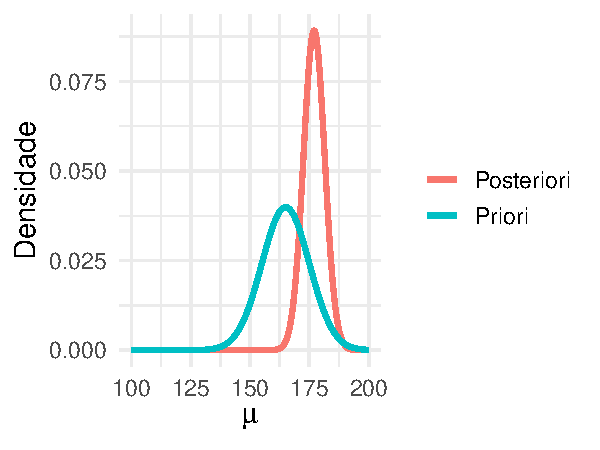
\includegraphics[width=\maxwidth]{./figures/normal_normal-1} 

}

\caption[Distribuições a priori e a posteriori (depois de observamos um indivíduo com 1,8m) para a altura média de um brasileiro]{Distribuições a priori e a posteriori (depois de observamos um indivíduo com 1,8m) para a altura média de um brasileiro}\label{fig:normal_normal}
\end{figure}

\end{knitrout}

\end{example}

A seguir, consideraremos o caso em que
$\mu$ é conhecido e $\tau^{2}$ é desconhecido.
\begin{lemma}
 Se $\mu$ é conhecido e
 $X|\tau^{2} \sim \text{N}(\mu,\tau^{2})$, então
 \begin{align*}
  \mathcal{P} = \left\{f: \mathbb{R} \rightarrow \mathbb{R}^{+}: f(\tau^{2}) = K \cdot \left(\tau^{2}\right)^{\alpha-1} \cdot \exp(-\beta \tau^{2}) \right\}
 \end{align*}
 é conjugada de $f(x|\tau^{2})$.
 Note que todas as densidades em $\mathcal{P}$ são
 da forma $\text{Gamma}(\alpha,\beta)$.
 Também, se $\tau^{2} \sim \text{Gamma}(\alpha,\beta)$,
 então
 \begin{align*}
  \tau^{2}|X \sim \text{Gamma}\left(\alpha+\frac{1}{2},
  \beta+\frac{(X-\mu)^{2}}{2}\right)
 \end{align*}
\end{lemma}

\begin{proof}
 \begin{align*}
  f(\tau^{2}) \cdot f(x|\mu)
  &= K \cdot \left(\tau^{2}\right)^{\alpha-1} \cdot \exp(-\beta \tau^{2}) \cdot \frac{\tau}{\sqrt{2\pi}} \cdot \exp\left(-\frac{\tau^{2}(x-\mu)^{2}}{2}\right)
  \nonumber \\
  &\propto \left(\tau^{2}\right)^{\alpha-1} \cdot \tau \cdot \exp(-\beta \tau^{2}) \cdot \exp\left(-\frac{\tau^{2}(x-\mu)^{2}}{2}\right) \\
  &= \left(\tau^{2}\right)^{\alpha+\frac{1}{2}-1} \cdot \exp\left(-\left(\beta+\frac{(x-\mu)^{2}}{2}\right)\tau^{2}\right) \in \mathcal{P}
 \end{align*}
 Também observe que $f(\tau^{2}) \cdot f(x|\tau^{2})$ é
 proporcional à densidade de uma Gamma com parâmetros
 $\alpha+\frac{1}{2}$ e
 $\left(\beta+\frac{(x-\mu)^{2}}{2}\right)$. Portanto,
 \begin{align*}
  \tau^{2}|X \sim \text{Gamma}\left(\alpha+\frac{1}{2},
  \beta+\frac{(x-\mu)^{2}}{2}\right).
 \end{align*}
\end{proof}

Finalmente, prosseguimos ao caso em que
tanto $\mu$ quanto $\tau^{2}$ são desconhecidos
\begin{lemma}
 \label{lemma:conjugate_normal_mean_precision}
 Se $X|\mu,\tau^{2} \sim \text{N}(\mu,\tau^{2})$,
 então
 \begin{align*}
  \mathcal{P} = \left\{f: \mathbb{R} \rightarrow \mathbb{R}^{+}: f(\mu) = K \cdot (\tau^{2})^{\alpha-1}\exp(-\beta \tau^{2})\exp\left(-\frac{\lambda\tau^{2}(\mu-\mu_{0})^{2}}{2}\right)\right\}
 \end{align*}
 é conjugada de $f(x|\mu,\tau^{2})$.
 As densidades em $\mathcal{P}$ pertencem à
 família bivariada Normal-Gamma com parâmetros
 $(\mu_{0},\lambda,\alpha,\beta)$. Note que se 
 $(\mu,\tau^{2})$ tem distribuição Normal-Gamma,
 então $\mu$ e $\tau^{2}$ não são independentes.
 De fato, se $(\mu,\tau^{2}) \sim \text{Normal-Gamma}(\mu_{0},\lambda,\alpha,\beta)$, então temos:
 \begin{align*}
  \tau^{2} \sim \text{Gamma}(\alpha, \beta) \\
  \mu|\tau^{2} \sim \text{Normal}(\mu_{0},\lambda \tau^{2})
 \end{align*}
 Também, se $(\mu,\tau^{2}) \sim \text{Normal-Gamma}(\alpha,\beta,\mu_{0},\lambda)$, então
 \begin{align*}
  (\mu,\tau^{2})|X \sim \text{Normal-Gamma}\left(\frac{(\lambda\mu_{0}+X)}{\lambda+1}, \lambda+1, \alpha+\frac{1}{2}, \beta + \frac{\lambda(\mu_{0}-X)^{2}}{2(\lambda+1)} \right)
 \end{align*}
\end{lemma}

\begin{proof}
 Note que, nos passos a seguir, tanto
 $\mu$ quanto $\tau^{2}$ são desconhecidos.
 Assim, expressões que dependam de
 quaisquer destes parâmetros não são constantes.
 \begin{align}
  \label{eqn:conjugate_normal_mean_variance_1}
  f(\mu,\tau^{2}|x)
  &\propto f(\mu,\tau^{2})f(x|\mu,\tau^{2})	\nonumber \\
  &= K \cdot (\tau^{2})^{\alpha-1}\exp(-\beta \tau^{2})\exp\left(-\frac{\lambda\tau^{2}(\mu-\mu_{0})^{2}}{2}\right) \cdot \frac{\tau}{\sqrt{2\pi}}\exp\left(-\frac{\tau^{2}(x-\mu)^{2}}{2}\right) \nonumber \\
  &\propto (\tau^{2})^{\alpha+\frac{1}{2}-1} \cdot \exp(-\beta \tau^{2}) \cdot \exp\left(-\frac{\lambda\tau^{2}(\mu^{2}-2\mu\mu_{0}+\mu_{0}^{2})}{2}\right) \cdot \exp\left(-\frac{\tau^{2}(x^{2}-2x\mu+\mu^{2})}{2}\right)	\nonumber \\
  &= (\tau^{2})^{\alpha+\frac{1}{2}-1} \cdot \exp\left(-\left(\beta + \frac{x^{2}}{2} + \frac{\lambda\mu_{0}^{2}}{2}\right)\tau^{2}\right) \cdot \exp\left(-\frac{\lambda\tau^{2}\mu^{2}-2\lambda\tau^{2}\mu\mu_{0}+\tau^{2}\mu^{2}-2\tau^{2}x\mu}{2}\right) \nonumber \\
  &= (\tau^{2})^{\alpha+\frac{1}{2}-1} \cdot \exp\left(-\left(\beta + \frac{x^{2}}{2} + \frac{\lambda\mu_{0}^{2}}{2}\right)\tau^{2}\right) \cdot \exp\left(-\frac{(\lambda+1)\tau^{2}\mu^{2}-2(\lambda\tau^{2}\mu_{0}+\tau^{2}x)\mu}{2}\right)
 \end{align}
 Similarmente ao caso em que $\tau^{2}$ é conhecido,
 desejamos completar o quadrado em função de
 $\mu$ para obter o formato da distribuição normal.
 Usamos novamente a \cref{eqn:conjugate_normal_2} para
 obter
 \begin{align*}
  \begin{cases}
   a^{2} &= (\lambda+1)\tau^{2} \\
   2ab &= 2(\lambda\tau^{2}\mu_{0}+\tau^{2}x)
  \end{cases}
 \end{align*}
 e obtemos
 \begin{align}
  \label{eqn:conjugate_normal_mean_variance_2}
  \begin{cases}
   a &= \sqrt{\lambda+1} \cdot \tau \\
   b &= \frac{\tau(\lambda\mu_{0}+x)}{\sqrt{\lambda+1}}
  \end{cases}
 \end{align}
 Substituindo a
 \cref{eqn:conjugate_normal_mean_variance_2}
 em \cref{eqn:conjugate_normal_mean_variance_1}, obtemos:
 \begin{align*}
  f(\mu,\tau^{2}|x) &\propto (\tau^{2})^{\alpha+\frac{1}{2}-1} \cdot \exp\left(-\left(\beta + \frac{x^{2}}{2} + \frac{\lambda\mu_{0}^{2}}{2}\right)\tau^{2}\right) \cdot \exp\left(-\frac{a^{2}\mu^{2}-2ab\mu}{2}\right) \\
  &= (\tau^{2})^{\alpha+\frac{1}{2}-1} \cdot \exp\left(-\left(\beta + \frac{x^{2}}{2} + \frac{\lambda\mu_{0}^{2}}{2}\right)\tau^{2}\right) \cdot \exp\left(-\frac{a^{2}\mu^{2}-2ab\mu+b^{2}}{2}\right) \cdot \exp\left(\frac{b^{2}}{2}\right) \\
  &= (\tau^{2})^{\alpha+\frac{1}{2}-1} \cdot \exp\left(-\left(\beta + \frac{x^{2}}{2} + \frac{\lambda\mu_{0}^{2}}{2}\right)\tau^{2} + \frac{b^{2}}{2}\right) \cdot \exp\left(-\frac{a^{2}\left(\mu-\frac{b}{a}\right)^{2}}{2}\right) \\
  &= (\tau^{2})^{\alpha+\frac{1}{2}-1} \cdot \exp\left(-\left(\beta + \frac{x^{2}}{2} + \frac{\lambda\mu_{0}^{2}}{2}\right)\tau^{2} + \frac{\tau^{2} (\lambda\mu_{0}+x)^{2}}{2(\lambda+1)}\right) \cdot \exp\left(-\frac{a^{2}\left(\mu-\frac{b}{a}\right)^{2}}{2}\right) \\
  &= (\tau^{2})^{\alpha+\frac{1}{2}-1} \cdot \exp\left(-\left(\beta + \frac{x^{2}}{2} + \frac{\lambda\mu_{0}^{2}}{2}\right)\tau^{2} + \frac{\tau^{2} (\lambda\mu_{0}+x)^{2}}{2(\lambda+1)}\right) \cdot \exp\left(-\frac{a^{2}\left(\mu-\frac{b}{a}\right)^{2}}{2}\right) \\
  &= (\tau^{2})^{\alpha+\frac{1}{2}-1} \cdot \exp\left(-\left(\beta + \frac{\lambda(\mu_{0}-x)^{2}}{2(\lambda+1)}\right)\tau^{2}\right) \cdot \exp\left(-\frac{a^{2}\left(\mu-\frac{b}{a}\right)^{2}}{2}\right)	\\
  &= (\tau^{2})^{\alpha+\frac{1}{2}-1} \cdot \exp\left(-\left(\beta + \frac{\lambda(\mu_{0}-x)^{2}}{2(\lambda+1)}\right)\tau^{2}\right) \cdot \exp\left(-\frac{(\lambda+1)\tau^{2}\left(\mu-\frac{(\lambda\mu_{0}+x)}{\lambda+1}\right)^{2}}{2}\right) \in \mathcal{P}
 \end{align*}
 Do resultado acima, podemos concluir que
 \begin{align*}
  (\mu,\tau^{2})|X \sim \text{Normal-Gamma}\left(\frac{(\lambda\mu_{0}+X)}{\lambda+1}, \lambda+1, \alpha+\frac{1}{2}, \beta + \frac{\lambda(\mu_{0}-X)^{2}}{2(\lambda+1)} \right)
 \end{align*}
\end{proof}


\begin{example}
 Considere novamente o Exemplo
 \ref{ex:altura}, mas vamos agora assumir 
 que a altura de um brasileiro selecionado ao acaso, 
 $X$, é tal que
 $X|\mu \sim N(\mu,\tau^2)$, 
 com $\tau^2$ desconhecido.
 Agora precisamos fazer a inferência simultaneamente 
 para $\mu$ e $\tau^2$
 Para tanto, vamos assumir que
 $(\mu,\tau^2) \sim \mbox{Normal-Gamma}(1.65,1,6,0.05)$.
 Como $x=1.8$,
 $(\mu,\tau^2)|x \sim 
 \mbox{Normal-Gamma}(1.725, 2, 6.5, 0.055625)$. 
 A Figura \ref{fig:normal_gamma} mostra 
 a distribuição a priori e 
 a distribuição a posteriori 
 para essa observação. 

\begin{knitrout}
\definecolor{shadecolor}{rgb}{0.969, 0.969, 0.969}\color{fgcolor}\begin{kframe}
\begin{alltt}
\hlkwd{library}\hlstd{(ggplot2)}
\hlkwd{library}\hlstd{(patchwork)}

\hlkwd{set.seed}\hlstd{(}\hlnum{0}\hlstd{)}
\hlstd{sigma} \hlkwb{<-} \hlnum{0.075}
\hlstd{mu} \hlkwb{<-} \hlnum{1.70}
\hlcom{# X ~ N(mu, sigma)}
\hlstd{altura} \hlkwb{<-} \hlnum{1.80}

\hlstd{atualiza} \hlkwb{<-} \hlkwa{function}\hlstd{(}\hlkwc{hparam}\hlstd{,} \hlkwc{x}\hlstd{)}
\hlstd{\{}
  \hlkwd{list}\hlstd{(}
    \hlkwc{mu0} \hlstd{= (hparam}\hlopt{$}\hlstd{lambda}\hlopt{*}\hlstd{hparam}\hlopt{$}\hlstd{mu0}\hlopt{+}\hlstd{x)}\hlopt{/}\hlstd{(hparam}\hlopt{$}\hlstd{lambda}\hlopt{+}\hlnum{1}\hlstd{),}
    \hlkwc{lambda} \hlstd{= hparam}\hlopt{$}\hlstd{lambda} \hlopt{+} \hlnum{1}\hlstd{,}
    \hlkwc{alpha} \hlstd{= hparam}\hlopt{$}\hlstd{alpha} \hlopt{+} \hlnum{.5}\hlstd{,}
    \hlkwc{beta} \hlstd{= hparam}\hlopt{$}\hlstd{beta} \hlopt{+}
      \hlstd{(hparam}\hlopt{$}\hlstd{lambda}\hlopt{*}\hlstd{(hparam}\hlopt{$}\hlstd{mu0}\hlopt{-}\hlstd{x)}\hlopt{^}\hlnum{2}\hlstd{)}\hlopt{/}\hlstd{(}\hlnum{2}\hlopt{*}\hlstd{(hparam}\hlopt{$}\hlstd{lambda}\hlopt{+}\hlnum{1}\hlstd{))}
  \hlstd{)}
\hlstd{\}}

\hlstd{hparam_prior} \hlkwb{<-} \hlkwd{list}\hlstd{(}
  \hlkwc{mu0} \hlstd{=} \hlnum{1.65}\hlstd{,}
  \hlkwc{lambda} \hlstd{=} \hlnum{1}\hlstd{,}
  \hlkwc{beta} \hlstd{=} \hlnum{0.05}\hlstd{,}
  \hlkwc{alpha} \hlstd{=} \hlnum{120}\hlopt{*}\hlnum{0.05}
\hlstd{)}

\hlstd{grid_bivariado} \hlkwb{<-} \hlkwd{expand.grid}\hlstd{(}
  \hlkwc{mu} \hlstd{=} \hlkwd{seq}\hlstd{(}\hlnum{1.4}\hlstd{,} \hlnum{1.8}\hlstd{,} \hlkwc{length.out} \hlstd{=} \hlnum{300}\hlstd{),}
  \hlkwc{tau2} \hlstd{=} \hlkwd{seq}\hlstd{(}\hlnum{60}\hlstd{,} \hlnum{200}\hlstd{,} \hlkwc{length.out} \hlstd{=} \hlnum{300}\hlstd{)}
\hlstd{)}

\hlcom{# retorna f(grid_bivariado|hparam)}
\hlstd{densidade} \hlkwb{<-} \hlkwa{function}\hlstd{(}\hlkwc{grid_bivariado}\hlstd{,} \hlkwc{hparam}\hlstd{)}
\hlstd{\{}
  \hlkwd{dgamma}\hlstd{(grid_bivariado}\hlopt{$}\hlstd{tau2,}
         \hlstd{hparam}\hlopt{$}\hlstd{alpha,}
         \hlstd{hparam}\hlopt{$}\hlstd{beta)}\hlopt{*}
    \hlkwd{dnorm}\hlstd{(grid_bivariado}\hlopt{$}\hlstd{mu,}
          \hlstd{hparam}\hlopt{$}\hlstd{mu0,}
          \hlkwd{sqrt}\hlstd{(}\hlnum{1}\hlopt{/}\hlstd{(hparam}\hlopt{$}\hlstd{lambda}\hlopt{*}\hlstd{grid_bivariado}\hlopt{$}\hlstd{tau2)))}
\hlstd{\}}

\hlstd{plot_densidade} \hlkwb{<-} \hlkwa{function}\hlstd{(}\hlkwc{grid_bivariado}\hlstd{,} \hlkwc{hparam}\hlstd{)}
\hlstd{\{}
  \hlstd{dados_plot} \hlkwb{<-} \hlkwd{data.frame}\hlstd{(}
    \hlkwc{mu} \hlstd{= grid_bivariado}\hlopt{$}\hlstd{mu,}
    \hlkwc{tau2} \hlstd{= grid_bivariado}\hlopt{$}\hlstd{tau2,}
    \hlkwc{densidade} \hlstd{=} \hlkwd{densidade}\hlstd{(grid_bivariado, hparam)}
  \hlstd{)}

  \hlkwd{ggplot}\hlstd{(dados_plot,}
         \hlkwd{aes}\hlstd{(mu, tau2,} \hlkwc{fill} \hlstd{= densidade))} \hlopt{+}
    \hlkwd{geom_raster}\hlstd{(}\hlkwc{interpolate} \hlstd{=} \hlnum{TRUE}\hlstd{)} \hlopt{+}
    \hlkwd{ggtitle}\hlstd{(}\hlkwd{paste0}\hlstd{(}\hlstr{"Prior"}\hlstd{))} \hlopt{+}
    \hlkwd{coord_cartesian}\hlstd{(}\hlkwc{xlim}\hlstd{=}\hlkwd{range}\hlstd{(grid_bivariado}\hlopt{$}\hlstd{mu),}
                    \hlkwc{ylim}\hlstd{=}\hlkwd{range}\hlstd{(grid_bivariado}\hlopt{$}\hlstd{tau2))} \hlopt{+}
    \hlkwd{scale_fill_gradientn}\hlstd{(}\hlkwc{colours} \hlstd{=} \hlkwd{terrain.colors}\hlstd{(}\hlnum{100}\hlstd{))} \hlopt{+}
    \hlkwd{theme_bw}\hlstd{()} \hlopt{+}
    \hlkwd{theme}\hlstd{(}\hlkwc{axis.text}\hlstd{=}\hlkwd{element_text}\hlstd{(}\hlkwc{size}\hlstd{=}\hlnum{18}\hlstd{),}
          \hlkwc{axis.title}\hlstd{=}\hlkwd{element_text}\hlstd{(}\hlkwc{size}\hlstd{=}\hlnum{20}\hlstd{,}\hlkwc{face}\hlstd{=}\hlstr{"bold"}\hlstd{))} \hlopt{+}
    \hlkwd{xlab}\hlstd{(}\hlkwd{expression}\hlstd{(mu))} \hlopt{+}
    \hlkwd{ylab}\hlstd{(}\hlkwd{expression}\hlstd{(tau}\hlopt{^}\hlnum{2}\hlstd{))}
\hlstd{\}}

\hlstd{aux1} \hlkwb{=} \hlkwd{plot_densidade}\hlstd{(grid_bivariado, hparam_prior)}
\hlstd{aux2} \hlkwb{=} \hlkwd{plot_densidade}\hlstd{(grid_bivariado,}
                      \hlkwd{atualiza}\hlstd{(hparam_prior, altura))}
\hlstd{aux1} \hlopt{/} \hlstd{aux2}
\end{alltt}
\end{kframe}\begin{figure}[t]

{\centering 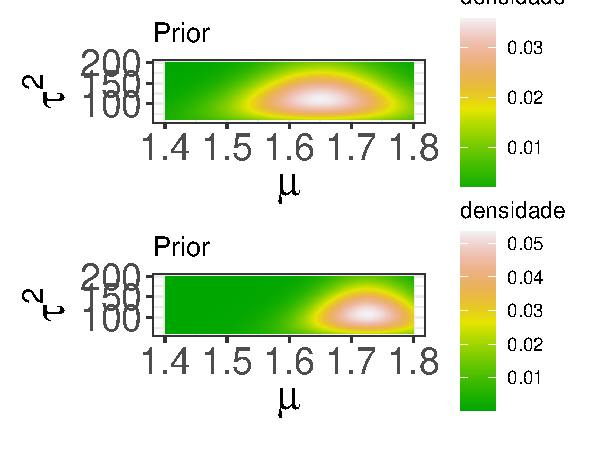
\includegraphics[width=\maxwidth]{./figures/normal_gamma-1} 

}

\caption[Distribuições a priori e a posteriori (depois de observamos um indivíduo com 1,8m) para a altura média de um brasileiro]{Distribuições a priori e a posteriori (depois de observamos um indivíduo com 1,8m) para a altura média de um brasileiro}\label{fig:normal_gamma}
\end{figure}

\end{knitrout}
\end{example}

\subsubsection*{Exercícios}

\begin{exercise}
 \label{ex:conjugate-normal-normal}
 Considere que, dado $\mu$,
 $X_{1},\ldots,X_{n}$ são i.i.d. e
 $X_{i} \sim N(\mu,\tau^{2})$, com
 $\tau^{2}$ conhecido. Se
 $\mu \sim N(\mu_{0},\tau_{0}^{2})$, então:
 \begin{enumerate}[label=(\alph*)]
  \item Ache a posteriori para
  $\mu|X_{1},\ldots,X_{n}$.
  \item Determine 
  $\lim_{n \rightarrow \infty}\E[\mu|X_{1},\ldots,X_{n}]$.
  \item Determine
  $\lim_{n \rightarrow \infty}\V[\mu|X_{1},\ldots,X_{n}]$.
  \item Interprete em suas próprias palavras os
  resultados obtidos nos itens anteriores.
 \end{enumerate}
\end{exercise}

\solution{\textbf{Solução}:
 \begin{enumerate}[label=(\alph*)]
  \item
  \begin{align*}
   f(\mu) \cdot f(x_{1},\ldots,x_{n}|\mu)
   &= f(\mu)\prod_{i=1}^{n}{f(x_{i}|\mu)} \\
   &\propto \exp\left(-\frac{\tau_{0}^{2}(\mu-\mu_{0})^{2}}{2}\right) \cdot \prod_{i=1}^{n}{\exp\left(-\frac{\tau^{2}(x_{i}-\mu)^{2}}{2}\right)} \\
   &= \exp\left(-\frac{\tau_{0}^{2}\mu^{2}-2\tau_{0}^{2}\mu\mu_{0}+\tau_{0}^{2}\mu_{0}^{2}}{2}\right) \cdot \exp\left(-\frac{n\tau^{2}\mu^{2}-2\tau^{2}\mu \sum_{i=1}^{n}{x_{i}}+ \tau^{2}\sum_{i=1}^{n}{x_{i}^{2}}}{2}\right)	\nonumber \\
   &\propto \exp\left(-\frac{\tau_{0}^{2}\mu^{2}-2\tau_{0}^{2}\mu\mu_{0}+n\tau^{2}\mu^{2}-2n\tau^{2}\mu \bar{x}}{2}\right) \\
   &= \exp\left(-\frac{(\tau_{0}^{2}+n\tau^{2})\mu^{2}-2(\tau_{0}^{2}\mu_{0}+n\tau^{2}\bar{x})\mu}{2}\right)
  \end{align*}
  Realizando uma substituição de acordo com a
  \cref{eqn:conjugate_normal_2}, obtemos
  \begin{align*}
   \begin{cases}
    a^{2} &= \tau_{0}^{2}+n\tau^{2} \\
    2ab &= 2(\tau_{0}^{2}\mu_{0}+n\tau^{2}\bar{x})
   \end{cases}
  \end{align*}
  e
  \begin{align}
   \begin{cases}
    a &= \sqrt{\tau_{0}^{2}+n\tau^{2}} \\
    b &= \frac{\tau_{0}^{2}\mu_{0}+n\tau^{2}\bar{x}}
    {\sqrt{\tau_{0}^{2}+n\tau^{2}}}
   \end{cases}
  \end{align}
  Realizando esta substituição na
  \cref{eqn:conjugate_normal_1}, obtemos:
  \begin{align*}
   f(\mu) \cdot f(x|\mu)
   &\propto \exp\left(-\frac{a^{2}\mu^{2}
   -2ab\mu}{2}\right) \\
   &\propto \exp\left(-\frac{a^{2}\mu^{2}
   -2ab\mu+b^{2}}{2}\right)
   & \exp(b^{2}/2) \text{ é constante} \\
   &= \exp\left(-\frac{(a\mu-b)^{2}}{2}\right)
   & \cref{eqn:conjugate_normal_2} \\
   &= \exp\left(-\frac{a^{2}\left(\mu
   -\frac{b}{a}\right)^{2}}{2}\right) \in \mathcal{P}
  \end{align*}
  Também observe que $f(\mu) \cdot f(x|\mu)$ é
  proporcional à densidade de uma normal com
  $\mu=\frac{b}{a}$ e $\tau^{2}=a^{2}$.
  Substituindo os valores obtidos na   
  \cref{eqn:conjugate_normal_3} temos que
  \begin{align*}
   \mu|X_{1},\ldots,X_{n} \sim
   N\left(\frac{\tau_{0}^{2}\mu_{0}+n\tau^{2}\bar{x}}{\tau_{0}^{2}+n\tau^{2}},\tau_{0}^{2}+n\tau^{2}\right)
  \end{align*}

  \item
  \begin{align*}
   \lim_{n \rightarrow \infty}E[\mu|X_{1},\ldots,X_{n}]	
   &= \lim_{n \rightarrow \infty}
   \frac{\tau_{0}^{2}\mu_{0}+n\tau^{2}\bar{X}}
   {\tau_{0}^{2}+n\tau^{2}} \\
   &= \lim_{n \rightarrow \infty}
   \frac{\tau_{0}^{2}\mu_{0}/n +\tau^{2}\bar{X}}
   {\tau_{0}^{2}/n +\tau^{2}} = \bar{X} \\
  \end{align*}

  \item 
  \begin{align*}
   \lim_{n \rightarrow \infty}
   \V[\mu|X_{1},\ldots,X_{n}]
   &= \lim_{n \rightarrow \infty}
   \frac{1}{\tau_{0}^{2}+n\tau^{2}} = 0
  \end{align*}
 \end{enumerate}
}{}

\begin{exercise}
 Considere que, dado $\tau^{2}$,
 $X_{1},\ldots,X_{n}$ são i.i.d. e
 $X_{i} \sim N(\mu,\tau^{2})$, com
 $\mu$ conhecido. Considere que
 $\tau^{2} \sim \text{Gamma}(\alpha,\beta)$.
 \begin{enumerate}[label=(\alph*)]
  \item Ache a posteriori para
  $\tau^{2}|X_{1},\ldots,X_{n}$.
  \item Derive $\lim_{n \rightarrow \infty}\E[\tau^{2}|X_{1},\ldots,X_{n}]$.
  \item Interprete em suas próprias palavras os
  resultados obtidos nos itens anteriores.
 \end{enumerate}
\end{exercise}

\solution{\textbf{Solução}:
 \begin{enumerate}[label=(\alph*)]
  \item
  \begin{align*}
   f(\tau^{2}|x_{1},\ldots,x_{n})
   &\propto f(\tau^{2})
   f(x_{1},\ldots,x_{n}|\tau^{2}) \\
   &= f(\tau^{2})\prod_{i=1}^{n}{f(x_{i}|\tau^{2})}	\\
   &\propto \left(\tau^{2}\right)^{\alpha-1} \cdot \exp\left(-\beta \tau^{2}\right) \cdot \tau^{n} \cdot \prod_{i=1}^{n}{\exp\left(-\frac{\tau^{2}(x_{i}-\mu)^{2}}{2}\right)} \\
   &= \left(\tau^{2}\right)^{\alpha+\frac{n}{2}-1} \cdot \exp\left(-\left(\beta+ \frac{\sum_{i=1}^{n}{(x_{i}-\mu)^{2}}}{2}\right)\tau^{2}\right)
  \end{align*}
  Portanto,
  \begin{align*}
   \tau^{2}|X_{1},\ldots,X_{n} \sim
   \text{Gamma}\left(\alpha+\frac{n}{2},
   \beta+\frac{\sum_{i=1}^{n}{(x_{i}-\mu)^{2}}}{2}\right)
  \end{align*}
  \item
  \begin{align*} 
   \limn\E[\tau^{2}|X_{1},\ldots,X_{n}]
   &= \lim_{n \rightarrow \infty}
   \frac{\alpha+\frac{n}{2}}
   {\beta+ \frac{\sum_{i=1}^{n}{(X_{i}-\mu)^{2}}}{2}} \\
   &= \limn\frac{n}{\sum_{i=1}^{n}{(X_{i}-\mu)^{2}}}
   = \tau^2
  \end{align*}
 \end{enumerate}
}{}

\subsubsection{A família exponencial}

A família exponencial é uma generalização de 
diversas famílias de distribuições.

\begin{definition}
 \label{defn:exponential-family}
 Dizemos que, dado um vetor de parâmetros $\theta$,
 um vetor de dados, $X$, 
 tem distribuição pertencente à família exponencial se o suporte de $x$ não
 depende de $\theta$ e se
 \begin{align*}
  f(x|\theta) 
  &= h(x) \exp\left(g(\theta) \cdot T(x)
  - A(\theta)\right)
 \end{align*}
 onde $g(\theta)$ e $T(x)$ são
 funções multivariadas dos parâmetros e dos dados.
\end{definition}

Note que, para cada valor de $\theta$,
$A(\theta)$ é o valor que faz com que
$f(x|\theta)$ integre $1$.
Assim, $A(\theta)$ é completamente especificado
em função dos demais elementos da família exponencial.

\begin{example}
 \label{example:exponential_family_binomial}
 Considere que $X|\theta \sim \text{Binomial}(n,\theta)$.
 \begin{align*}
  f(x|\theta)
  &= {n \choose x}\theta^{x}(1-\theta)^{n-x} \\
  &= {n \choose x}\exp\left(x\log(\theta)
  +(n-x)\log(1-\theta)\right) \\
  &= {n \choose x}\exp\left(x \cdot \log\left(\frac{\theta}{1-\theta}\right) +n\log(1-\theta)\right)
 \end{align*}
 Portanto, $f(x|\theta)$ pertence à
 família exponencial, tomando-se 
 \begin{align*}
  \begin{cases}
   h(x) &= {n \choose x} \\
   T(X) &= x \\
   g(\theta) 
   &= \log\left(\frac{\theta}{1-\theta}\right) \\
   A(\theta) &= -n\log(1-\theta)
  \end{cases}
 \end{align*}
\end{example}

\begin{example}
 Considere que $\theta=(\mu,\tau^{2})$ e
 $X|\theta \sim \text{Normal}(\mu,\tau^{2})$.
 \begin{align*}
  f(x|\mu,\tau^{2})
  &= \frac{\tau}{\sqrt{2\pi}}\exp\left(-\frac{\tau^{2}(x-\mu)^{2}}{2}\right) \\
  &= \frac{1}{\sqrt{2\pi}}\exp\left(-\frac{\tau^{2}x^{2}-2\tau^{2}x\mu +\tau^{2}\mu^{2}}{2} +\log(\tau)\right) \\
  &= \frac{1}{\sqrt{2\pi}}\exp\left((x,-x^{2}/2) \cdot (\tau^{2}\mu, \tau^{2}) -\left(\frac{\tau^{2}\mu^{2}}{2}-\log(\tau)\right)\right)
 \end{align*}
 Portanto, $f(x|\theta)$ pertence à
 família exponencial, tomando-se 
 \begin{align*}
  \begin{cases}
   h(x) &= \frac{1}{\sqrt{2\pi}} \\
   T(X) &= (x,-x^{2}/2) \\
   g(\theta) &= (\tau^{2}\mu, \tau^{2}) \\
   A(\theta) &= \left(\frac{\tau^{2}\mu^{2}}{2}
   -\log(\tau)\right)
  \end{cases}
 \end{align*}
\end{example}

Muitas outras distribuições pertencem à
família exponencial. Por exemplo, a Binomial-Negativa,
a Poisson, a Multinomial, a Hipergeométrica,
a Geométrica, a log-Normal, a Exponencial,
a Gamma, a Gamma-Inversa, a Beta, a Weibull e a Laplace.

Além de incluir diversas distribuições,
a família exponencial também apresenta
propriedades importantes. No contexto desta seção, 
podemos derivar a família conjugada para
um membro da família exponencial.

\begin{lemma}
 \label{lemma:exponential-family-conjugate}
 Se $f(x|\theta)$ faz parte da família exponencial,
 isto é, $f(x|\theta) = h(x) \exp\left(g(\theta) \cdot T(x) - A(\theta)\right)$, então
 \begin{align*}
  \mathcal{P} = \left\{f(\theta): f(\theta) 
  = K \cdot \exp\left(-\alpha A(\theta) + g(\theta) \cdot \beta\right) \right\}
 \end{align*}
 é conjugada a $f(x|\theta)$.
\end{lemma}

\begin{proof}
 Note que
 \begin{align*}
  f(\theta)f(x|\mu)
  &\propto \exp\left(-\alpha A(\theta)
  +g(\theta) \cdot \beta\right) \cdot h(x)
  \cdot \exp\left(g(\theta) \cdot T(x)
  -A(\theta)\right) \\
  &\propto \exp\left(-(\alpha+1)A(\theta)
  +g(\theta) \cdot (\beta+T(x))\right) \in \mathcal{P}
 \end{align*}
 Portanto, $\mathcal{P}$ é conjugada de $f(x|\theta)$.
 Similarmente, para o caso em que
 $X_{1},\ldots,X_{n}$ são i.i.d. dado $\theta$,
 obtemos
 \begin{align*}
  f(\theta)f(x_{1},\ldots,x_{n}|\mu)
  &=f(\theta)\prod_{i=1}^{n}{f(x_{i}|\theta)} \\
  &\propto \exp\left(-\alpha A(\theta)
  +g(\theta) \cdot \beta\right) \cdot \prod_{i=1}^{n}
  {\exp\left(g(\theta) \cdot T(x_{i})
  -A(\theta)\right)} \\
  &\propto \exp\left(-(\alpha+n)A(\theta)
  +g(\theta) \cdot \left(\beta+\sum_{i=1}^{n}
  {T(x_{i})}\right)\right) \in \mathcal{P}
 \end{align*}
\end{proof}

\begin{example}
 \label{example:exponential-family-binomial}
 Considere que
 $X|\theta \sim \text{Binomial}(n,\theta)$.
 Vimos no \cref{example:exponential_family_binomial}
 que $f(x|\theta)$ pertence à família exponencial.
 Portanto, temos que
 \begin{align*}
  \mathcal{P} = \{f(\theta) =K
  \cdot \exp\left(-\alpha A(\theta)
  +g(\theta) \cdot \beta \right) \}
 \end{align*}
 é conjugada de $f(x|\theta)$.
 Substituindo os termos encontrados no
 \cref{example:exponential_family_binomial}, obtemos
 \begin{align*}
  \mathcal{P} &= \left\{f(\theta) = K \cdot \exp\left(\alpha n\log(1-\theta) +\log\left(\frac{\theta}{1-\theta}\right) \cdot \beta \right) \right\} \\
  &= \{f(\theta) = K(1-\theta)^{n\alpha-\beta} \theta^{\beta} \}
 \end{align*}
 Assim encontramos que a família Beta é
 conjugada da Binomial, assim como na
 \cref{sec:conjugate_beta_binomial}.
 Observe que, para que seja possível obter
 $\int{f(\theta)d\theta}=1$, é necessário que
 $n\alpha > \beta$ e $\beta > 0$. 
\end{example}

Ao aplicar o \cref{lemma:exponential-family-conjugate},
nem sempre é imediato quais valores de
$\alpha$ e $\beta$ são tais que
$f(\theta)$ é integrável.
No \cref{example:exponential-family-binomial}
verificamos que, para obter esta condição, era
necessário que $n\alpha > \beta$ e $\beta > 0$.
Esta análise é generalizada por um teorema em \citet{Diaconis1979} que é descrito a seguir.

\begin{theorem}
 \label{theorem:exponencial-propriety}
 Considere que $X \in \chi$,
 $\theta \in \mathbb{R}^{d}$ e
 $f(x|\theta)$ está na forma canônica da
 família exponencial, isto é,
 $f(x|\theta) = h(x) \exp\left(\theta \cdot T(x) - A(\theta)\right)$.
 A função $f(\theta) = \exp\left(-\alpha A(\theta) +\theta \cdot \beta \right)$
 é integrável se e somente se $\alpha > 0$ e
 $\frac{\beta}{\alpha} \in \text{Interior}[\text{Conv}[T[\chi]]]$.
\end{theorem}

\begin{example}
 Considere que
 $X|\theta \sim \text{Poisson}(\theta)$. Obtemos,
 \begin{align*}
  f(x|\theta)
  &= \frac{\exp(-\theta)\theta^{x}}{x!} \\
  &= (x!)^{-1} \exp(\log(\theta) \cdot x - \theta) \\
 \end{align*}
 Assim, definindo $\eta = \log(\theta)$, obtemos:
 \begin{align*}
  f(x|\eta)
  &= (x!)^{-1} \exp(\eta \cdot x - \exp(\eta))
 \end{align*}
 Conclua que $f(x|\eta)$ está na
 forma canônica da familia exponencial, tomando
 \begin{align*} 
  \begin{cases}
   h(x) &= (x!)^{-1} \\
   T(x) &= x \\
   A(\eta) &= \exp(\eta) \\
  \end{cases}
 \end{align*}
 Portanto, decorre do
 \cref{lemma:exponential-family-conjugate} que
 a seguinte familia é conjugada para $f(x|\eta)$
 \begin{align*}
  \mathcal{P} = \left\{f(\eta): f(\eta) \propto \exp(-\alpha\exp(\eta) + \eta \cdot \beta) \right\}
 \end{align*}
 Ademais, podemos aplicar o
 \cref{theorem:exponencial-propriety} para
 obter os valores de $\alpha$ e $\beta$ tais que
 $\exp(-\alpha\exp(\eta) + \eta \cdot \beta)$ é
 integrável. Obtemos que $\exp(-\alpha\exp(\eta) + \eta \cdot \beta)$ é integrável se e somente se
 $\alpha > 0$ e $\frac{\beta}{\alpha} \in \text{Interior}[\text{Conv}[T[\chi]]]$.
 Como $X|\theta \sim \text{Poisson}(\theta)$, obtemos
 $\chi = \mathbb{N}$.
 Assim, como $T(x) = x$, $T[\mathbb{N}] = \mathbb{N}$.
 Ademais, $\text{Conv}[\mathbb{N}] = \mathbb{R}^{+}$.
 Finalmente, $\text{Interior}[\mathbb{R}^+] = \mathbb{R}^{+}_{*}$.
 Portanto, $\text{Interior}[\text{Conv}[T[\chi]]] = \mathbb{R}^{+}_{*}$.
 Note que, se $\alpha > 0$, então
 $\frac{\beta}{\alpha} \in \mathbb{R}^{+}_{*}$
 se e somente se $\beta > 0$.
 Portanto, conclua do \cref{theorem:exponencial-propriety} que 
 $\exp(-\alpha\exp(\eta) + \eta \cdot \beta)$ é
 integrável se e somente $\alpha > 0$ e $\beta > 0$.
 Tomando a transformação $\log(\theta) = \eta$,
 obtemos que 
 $\big|\frac{d\log(\theta)}{d\theta}\big| \exp(-\alpha\theta + \log(\theta) \cdot \beta)$ é
 integrável se e somente se
 $\alpha > 0$ e $\beta > 0$. Assim,
 \begin{align*} 
  \mathcal{P}^{*} &= \left\{f(\theta):
  f(\theta) \propto \theta^{\beta-1}\exp(-\alpha \theta), \alpha > 0, \beta > 0\right\}
 \end{align*}
 é uma familia de distribuições integráveis.
 Ademais, decorre do
 \cref{lemma:exponential-family-conjugate} que
 $\mathcal{P}$ é conjugada para $f(x|\theta)$.
 Note que as densidades em $\mathcal{P}^{*}$
 correspondem à família de distribuições Gamma.
\end{example}

\subsubsection*{Exercícios}

\begin{exercise}
 O jogador $A$ acredita que a frequência com que 
 ela vence jogos de xadrez contra o jogador $B$
 segue uma distribuição $\text{Beta}(2,2)$.
 Em um torneio, o jogador $A$ joga quatro partidas contra
 o jogador $B$ até ganhar seu primeiro jogo.
 \begin{enumerate}[label=(\alph*)]
  \item Descreva os elementos do modelo estatístico Bayesiano.
  \item Antes de jogar contra $B$, em média quantas vezes
  o jogador $A$ acreditava que ele precisaria jogar
  até vencer contra o jogador $B$?
  \item Encontre a distribuição a posteriori para
 a frequência com que o jogador $A$ vence
 jogos contra o jogador $B$ após o torneio.
 \item Após o torneio, em média quantas partidas a mais
 o jogador $A$ acredita que precisaria jogar contra $B$
 para obter uma nova vitória?
 \end{enumerate}
\end{exercise}

\begin{exercise}
 Escolha duas de suas famílias de
 distribuições favoritas e descubra se
 elas pertencem ou não à família exponencial.
\end{exercise}

\begin{exercise}
 Se $X|\theta \sim \text{Geom}(\theta)$:
 \begin{enumerate}[label=(\alph*)]
  \item Mostre que $f(x|\theta)$ pertence à
  família exponencial.
  \item Ache a família conjugada para $f(x|\theta)$.
  \item Ache a posteriori para $\theta$ quando
  a priori é conjugada.
 \end{enumerate} 
\end{exercise}

\solution{\textbf{Solução}:
 \begin{enumerate}[label=(\alph*)]
  \item
  \begin{align*}
   f(x|\theta) &= \theta (1-\theta)^{x} \\
   &= \exp(\log(\theta) + \log(1-\theta)x) \\
   &= 1 \cdot \exp(\log(1-\theta) \cdot x
   +\log(\theta))
  \end{align*}
  Portanto, $f(x|\theta)$ pertence à
  família exponencial com:
  \begin{align*}
   \begin{cases}
    h(x) &= 1 \\
    g(\theta) &= \log(1-\theta) \\
    T(x) &= x \\
    A(\theta) &= -\log(\theta)
   \end{cases}
  \end{align*}
  
  \item
  \begin{align*}
   \mathcal{P}	&= \{f(\theta)
   =K \cdot (\exp(-A(\theta)))^{\alpha} \cdot \exp(g(\theta) \cdot \beta) \} \\
   &= \{f(\theta) 
   =K \cdot (\exp(\log(\theta)))^{\alpha} \cdot \exp(\log(1-\theta)\beta) \} \\
   &= \{f(\theta) =K \cdot \theta^{\alpha}
   (1-\theta)^{\beta}\}
  \end{align*}
  Portanto, a família Beta é conjugada a $f(x|\theta)$.
  \item
  \begin{align*}
   f(\theta|x)	&\propto f(\theta)f(x|\theta) \\
   &\propto \theta^{\alpha}(1-\theta)^{\beta}\theta (1-\theta)^{x} \\
   &= \theta^{\alpha+1}(1-\theta)^{\beta+x} \sim \text{Beta}(\alpha+2, \beta+x+1)
  \end{align*}
 \end{enumerate}
}{}

\begin{exercise}
 Se $X|\theta \sim \text{Exponencial}(\theta)$:
 \begin{enumerate}[label=(\alph*)]
  \item Mostre que $f(x|\theta)$ pertence à
  família exponencial.
  \item Ache a família conjugada para $f(x|\theta)$.
  \item Ache a posteriori para $\theta$ quando
  a priori é conjugada.
 \end{enumerate} 
\end{exercise}

\solution{\textbf{Solução}:
 \begin{enumerate}[label=(\alph*)]
  \item 
  \begin{align*}
   f(x|\theta)
   &= \theta \exp(-\theta x) \\
   &= 1 \cdot \exp(-\theta \cdot x +\log(\theta))
  \end{align*}
  Portanto, $f(x|\theta)$ pertence à
  família exponencial com:
  \begin{align*}
   \begin{cases}
    h(x) &= 1 \\
    g(\theta) &= -\theta \\
    T(x) &= x \\
    A(\theta) &= -\log(\theta)
   \end{cases}
  \end{align*}
  \item 
  \begin{align*}
   \mathcal{P}	&= \{f(\theta)
   =K \cdot (\exp(-A(\theta)))^{\alpha} \cdot \exp(g(\theta) \cdot \beta) \} \\
   &= \{f(\theta) 
   =K \cdot (\exp(\log(\theta)))^{\alpha} \cdot \exp(-\theta\beta) \} \\
   &= \{f(\theta) =K \cdot \theta^{\alpha}
   exp(-\theta \beta) \}
  \end{align*}
  Portanto, a família Gamma é conjugada a $f(x|\theta)$.
  \item 
  \begin{align*}
   f(\theta|x) &\propto f(\theta)f(x|\theta) \\
   &\propto \theta^{\alpha}\exp(-\theta \beta)
   \theta \exp(-\theta x) \\
   &= \theta^{\alpha+1}\exp(-\theta (\beta+x)
   \sim \text{Gamma}(\alpha+2, \beta+x)
  \end{align*}
 \end{enumerate}
}{}

\begin{exercise}
 Em uma população, a proporção de indivíduos com
 uma determinada doença é $\theta$.
 Considere que uma amostra de $100$ indivíduos é
 tomada da população. Para cada indivíduo, $i$,
 defina $Z_{i}$ como sendo a indicadora de que
 o indivíduo tem a doença.
 Um teste é realizado em cada um
 dos indivíduos da amostra.
 Este teste é tal que, se o indivíduo for doente,
 o teste acusa afirmativo certamente.
 Contudo, se o indivíduo não for doente,
 há uma probabilidade $0.1$ de um falso positivo.
 Para cada indivíduo, $i$, defina
 $X_{i}$ como sendo a indicadora de que
 o resultado do exame para o indivíduo $i$ foi positivo.
 Observou-se que $30$ indivíduos obtiveram
 o resultado positivo no teste.
 Note que as variáveis $Z_{i}$ não foram observadas.
 \begin{enumerate}[label=(\alph*)]
  \item Note que $X_{1}|\theta$ é uma Bernoulli.
  Use a lei da probabilidade total para mostrar que
  \begin{align*}
   X_{1}|\theta \sim \text{Bernoulli}(0.1 + 0.9\theta)
  \end{align*}
  \item Ache a distribuição de
  $\sum_{i=1}^{100}{X_{i}}|\theta$ e
  prove que ela pertence à família exponencial.
  \item Ache a família conjugada para
  $\sum_{i=1}^{100}{X_{i}}|\theta$.
  \item Tome uma priori na família conjugada para
  $\theta$ e ache a distribuição de
  $\theta|\sum_{i=1}^{100}{X_{i}}=30$.
 \end{enumerate}
\end{exercise}

\solution{\textbf{Solução}:
 \begin{enumerate}[label=(\alph*)]
  \item Como $X_{i} \in \{0,1\}$,
  $X_{i}$ segue uma distribuição Bernoulli.
  \begin{align*}
   \P(X_{i}=1|\theta)
   &= \P(X_{i}=1|Z_{i}=1,\theta)\P(Z_{i}=1|\theta)
   +\P(X_{i}=1|Z_{i}=0,\theta)\P(Z_{i}=0|\theta) \\
   &= \theta + 0.1(1-\theta) = 0.1 + 0.9\theta
  \end{align*}
  Portanto $X_{i}|\theta \sim \text{Bernoulli}(0.1+0.9\theta)$.
  \item Como, dado $\theta$,
  $X_{1}, \ldots, X_{n}$ são i.i.d. e
  $X_{1} \sim \text{Bernoulli}(0.1+0.9\theta)$, então
  $\sum_{i=1}^{n}{X_{i}}|\theta \sim \text{Binomial}(n,0.1+0.9\theta)$.
  \item
  \begin{align*}
   f(n\bar{x}|\theta)
   &= {n \choose n\bar{x}} (0.1+0.9\theta)^{n\bar{x}}
   (1-(0.1+0.9\theta))^{n(1-\bar{x})} \\
   &= {n \choose n\bar{x}} \exp\left(n\bar{x}\log\left(\frac{0.1+0.9\theta}{1-(0.1+0.9\theta)}\right) + n\log(1-(0.1+0.9\theta))\right)
  \end{align*}
  Portanto, $f(n\bar{x}|\theta)$ pertence à
  família exponencial, tomando
  \begin{align*}
   \begin{cases}
    h(n\bar{x}) &= {n \choose n\bar{x}}	\\
    T(n\bar{x}) &= n\bar{x} \\
    g(\theta) &= \log\left(\frac{0.1+0.9\theta}{1-(0.1+0.9\theta)}\right) \\
    A(\theta) &= -n\log(1-(0.1+0.9\theta))
   \end{cases}
  \end{align*}
  \item Decorre do 
  \cref{lemma:exponential-family-conjugate} que, 
  como $f(n\bar{x}|\theta)$ pertence à
  família exponencial, então
  \begin{align*}
   \mathcal{P} &= \{f(\theta) 
   =K \exp(-\alpha A(\theta)) \cdot \exp(g(\theta)
   \cdot \beta)\} \\
   &= \{f(\theta) 
   =K \left(1-(0.1+0.9\theta)\right)^{n\alpha} 
   \left(\frac{0.1+0.9\theta}{1-(0.1+0.9\theta)}\right)^{\beta}	\\
   &= \{f(\theta) 
   =K (0.1+0.9\theta)^{\gamma}(1-(0.1+0.9\theta))^{\delta}
  \end{align*}
  é conjugada para $f(n\bar{x}|\theta)$. Assim, se
  tomarmos $f(\theta) \in \mathcal{P}$, obtemos:
  \begin{align*}
   f(\theta|n\bar{x})
   &\propto f(\theta)f(n\bar{x}|\theta)	\\
   &\propto (0.1+0.9\theta)^{\gamma}(1-(0.1+0.9\theta))^{\delta}(0.1+0.9\theta)^{n\bar{x}}(1-(0.1+0.9\theta))^{n(1-\bar)} \\
   &= (0.1+0.9\theta)^{\gamma+n\bar{x}}(1-(0.1+0.9\theta))^{\delta+n(1-\bar{x})}
  \end{align*}
  Para achar a forma exata de
  $f(\theta|n\bar{x})$, tomamos
  \begin{align*}
   \int_{0}^{1}{K \cdot (0.1+0.9\theta)^{\gamma+n\bar{x}}(1-(0.1+0.9\theta))^{\delta+n(1-\bar{x})} d\theta} &= 1 \\
   \int_{0}^{1}{K y^{\gamma+n\bar{x}}(1-y)^{\delta+n(1-\bar{x})} 0.9^{-1} dy} &= 1 \\
   K = 0.9B^{-1}(\gamma+n\bar{x}+1,\delta+n(1-\bar{x})+1)
  \end{align*}
  \begin{align*}
   f(\theta|n\bar{x})
   &= 0.9B^{-1}(\gamma+n\bar{x}+1,\delta+n(1-\bar{x})+1)(0.1+0.9\theta)^{\gamma+n\bar{x}}(1-(0.1+0.9\theta))^{\delta+n(1-\bar{x})}
  \end{align*}
 \end{enumerate}
}{}

\begin{exercise}
 Considere que $X|\theta \sim \text{Bernoulli}(\theta)$.
 \begin{enumerate}[label=(\alph*)]
  \item Reparametrize esta  distribuição de $X|\theta$ para
  que se enquadra na forma canônica da família exponencial.
  \item Determine uma família conjugada para a reparametrização
  utilizando o \cref{lemma:exponential-family-conjugate}.
  \item Utilize o \cref{theorem:exponencial-propriety} para
  determinar as densidades na família encontrada no item acima.
 \end{enumerate}
\end{exercise}

\subsubsection{O processo de Dirichlet*}

Nas seções anteriores, consideramos que,
dado um conjunto de parâmetros, $\theta$,
$X_1, \ldots, X_n$ eram i.i.d. com
uma distribuição determinada por $\theta$.
Em outras palavras, 
para cada $\theta$ havia uma densidade
$f_{\theta}$ tal que
\begin{align*}
 f(x_1,\ldots,x_n|f_{\theta})
 &= \prod_{i=1}^{n}f_{\theta}(x_i)
\end{align*}
Neste tipo de modelo,
você atribuiu prioris sobre
$\theta$ (e, portanto, sobre $f_{\theta}$) que
eram convenientes computacionalmente.
Contudo, as possíveis distribuições que
$f_{\theta}$ podia assumir eram limitadas.
Por exemplo, na \cref{sec:conj-norm}
$f_{\theta}$ era necessariamente 
uma distribuição normal
com média e variância dadas por $\theta$.

Contudo, em alguns casos você poderá querer
que $f_{\theta}$ tenha como possíveis valores
uma classe mais geral.
Este é o tipo de problema que é estudado pela
estatística não-paramétrica.
A dificuldade da estatística não-paramétrica é
obter uma classe de $f_{\theta}$ que 
seja geral e, ainda assim, 
conveniente computacionalmente.
Uma maneira de obter este resultado é
pelo processo de Dirichlet, que
veremos a seguir.

Para definir o processo de Dirichlet,
ao invés de $f_{\theta}$, consideraremos
uma função de probabilidade aleatória
sobre $\mathbb{R}$, $P_{\theta}$.
Note que $P_{\theta}$ é uma função aleatória,
isto é, para cada $A \subset \mathbb{R}$,
$P_{\theta}(A)$ é uma variável aleatória.
Consideraremos também que, dado $P_{\theta}$,
$(X_1,\ldots,X_n)$ são i.i.d. com
distribuição dada por $P_{\theta}$, isto é,
\begin{align}
 \label{eq:pd-1}
 \P(X_1 \in A_1, \ldots, X_n \in A_n|P_{\theta})
 &= \prod_{i=1}^{n}P_{\theta}(A_i)
\end{align}

O processo de Dirichlet é 
uma distribuição sobre $P_{\theta}$ que 
faz com o suporte de $P_{\theta}$ possa ser
a familia de todas as distribuições univariadas.
O processo de Dirichlet tem como parâmetros
uma função de probabilidade sobre $\mathbb{R}$,
$P_0$, e $\alpha \in \mathbb{R}_{+}$. 
Ele é definido da seguinte forma:

\begin{definition}
 \label{def:pd}
 Dizemos que $P_{\theta}$ tem distribuição dada
 pelo processo de Dirichlet com parâmetros
 $P_0$ e $\alpha$ e escrevemos
 $P_{\theta} \sim \text{PD}(P_0, \alpha)$ se
 $P_{\theta}$ é uma função de probabilidade 
 com probabilidade $1$ e, também,
 para todo $d \in \mathbb{N}$ e
 partição finita de $\mathbb{R}$,
 $(B_i)_{1 \leq i \leq d}$,
 \begin{align*}
  (P_{\theta}(B_1), \ldots,P_{\theta}(B_d))
  & \sim \text{Dirichlet}
  (\alpha(P_0(B_1),\ldots, P_0(B_d)))
 \end{align*}
\end{definition}

Frente a uma definição de
processo estocástico como a \cref{def:pd},
existem algumas perguntas comumente feitas.
Por exemplo, existe de fato 
um processo estocástico que satisfaça
a \cref{def:pd}?
Também, qual é a probabilidade de que
$P_{\theta}$ seja efetivamente
uma função de probabilidade sobre $\mathbb{R}$?
Dentre outras referências, por exemplo
\citep{Ferguson1973,Sethuraman1994} mostram que
existe um processo estocástico que
satisfaz a \cref{def:pd} e que, 
com probabilidade 1, $P_{\theta}$ é
uma probabilidade sobre $\mathbb{R}$.

Para compreender o processo de Dirichlet,
podemos calcular algumas
de suas propriedades relevantes.
Por exemplo, para cada $x \in \mathbb{R}$,
podemos definir $F_{\theta}(x) 
:= \P_{\theta}((-\infty,x])$ e
$F_0(x) := \P_0((-\infty,x])$. Assim,
$F_{\theta}(x)$ é uma variável aleatória e
$F_0(x)$ é uma constante.
Pela definição do processo de Dirichlet,
\begin{align*}
 (P_{\theta}((-\infty,x]),P_{\theta}((x,\infty)))
 &\sim \text{Dirichlet}(\alpha P_0((-\infty,x]),
 \alpha P_0((x,\infty)))
\end{align*}
Dada a relação entra as distribuições Beta e
a Dirichlet, decorre diretamente que
\begin{align*}
 F_{\theta}(x) \sim \text{Beta}
(\alpha P_0((-\infty,x]), \alpha P_0((x,\infty)))
\end{align*}
Portanto, obtemos que,
para cada $x \in \mathbb{R}$,
\begin{align*}
 \E[F_{\theta}(x)] 
 &= F_0(x) \\
 \V[F_{\theta}(x)] 
 &= \frac{F_0(x)(1-F_0(x))}{1+\alpha}
\end{align*}
Assim, enquanto que
$P_0$ representa a tendência central
do processo de Dirichlet, 
$\alpha$ indica o quanto o processo
está concentrado em torno de $P_0$.
De fato, a distribuição marginal de $X$
é dada por $P_0$

\begin{lemma}
 \label{lemma:dp-marginal}
 Se $X|P_{\theta} \sim P_{\theta}$ e
 $P_{\theta} \sim \text{DP}(P_0, \alpha)$, então
 $X \sim P_0$.
\end{lemma}

\begin{proof}
 \begin{align*}
  \P(X \leq x) 
  &= \E[\P(X \leq x|P_{\theta})] \\
  &= \E[\P_{\theta}((-\infty,x])] \\
  &= P_0((\infty,x])
 \end{align*}
\end{proof}

Além de ser uma priori abrangente para $P_{\theta}$,
o processo de Dirichlet também é
conveniente computacionalmente.
Esta propriedade é apresentada a seguir e
acompanha a demonstração em
\citep{Ferguson1973}.

\begin{definition}[$\delta$ de Dirac]
 \label{defn:dirac}
 Para cada $x \in \mathbb{R}$,
 defina $\delta_x$ tal que
 $\delta_x = \I(x \in A)$.
\end{definition}

\begin{theorem}
 \label{thm:dirichlet_post}
 Se $P_{\theta} \sim DP(P_0, \alpha)$ e,
 dado $P_{\theta}$, $X$ tem distribuição $P_{\theta}$,
 então $P_{\theta}|X \sim DP\left(
 \frac{\alpha P_0 + \delta_{x}}
 {\alpha+1}, \alpha+1\right)$.
\end{theorem}

Para provar o \cref{thm:dirichlet_post},
alguns resultados sobre a distribuição
Dirichlet serão úteis.
Estes podem ser provados usando
técnicas comumente usadas para
vetores de variáveis aleatórias e
são enunciados a seguir.

\begin{definition}
 Considere que 
 $(Y_1,\ldots,Y_n)
 \sim \text{Dirichlet}(\alpha_1,\ldots,\alpha_n)$.
 Denotamos a função de densidade acumulada
 de $(Y_1,\ldots,Y_n)$ por
 $\mathcal{D}(y_1,\ldots,y_n|\alpha_1,\ldots,\alpha_n)$.
\end{definition}

\begin{lemma}
 \label{lemma:dirichlet-1}
 Se $(X_1,\ldots,X_n)$ são independentes,
 $X_i \sim \text{Gamma}(\alpha_i)$ e
 $S = \sum_{i=1}^n X_i$, então
 \begin{align*}
  \frac{\left(X_1, \ldots, X_n\right)}{S}
  & \sim \text{Dirichlet}(\alpha_1,\ldots,\alpha_n)
 \end{align*}
\end{lemma}

\begin{lemma}
 \label{lemma:dirichlet-2}
 Se $Y_1,\ldots,Y_n \sim \text{Dirichlet}$, então
 $(Y_1,\ldots,Y_{n-2},Y_{n-1}+Y_{n}) 
 \sim \text{Dirichlet}(\alpha_1,\ldots,\alpha_{n-2},
 \alpha_{n-1}+\alpha_n)$.
\end{lemma}

\begin{lemma}
 \label{lemma:dirichlet-3}
 Considere que
 $(Y_1,\ldots,Y_n)
 \sim \text{Dirichlet}(\alpha_1,\ldots,\alpha_n)$.
 \begin{align*}
  \E\left[Y_{n} \I(Y_{n-1}+Y_{n} \leq y_{n-1})
  \prod_{i < n-1} \I(Y_i \leq y_{i})\right]
  &= \frac{\alpha_n}{\sum_{i=1}^n \alpha_i}
  \mathcal{D}(y_1,\ldots,y_{n-1}|
  \alpha_1,\ldots,\alpha_{n-2},\alpha_{n-1}+\alpha_n+1)
 \end{align*}
\end{lemma}

\begin{proof}
 Defina $C = \bigcap_{i < n-1}\{Y_i \leq y_i\} 
 \cap \{Y_{n-1}+Y_{n} < y_{n-1}\} \cap 
 \{\sum_{i=1}^n Y_i = 1\}$,
 $\alpha^*_i = \alpha_i + \I(i=n)$, e
 $(Y^*_1,\ldots,Y^*_n) \sim \text{Dirichlet}
 (\alpha^*_1,\ldots,\alpha^*_n)$.
 \begin{align*}
  \E\left[Y_{n} \I(Y_{n-1}+Y_{n} \leq y_{n-1})
  \prod_{i < n-1} \I(Y_i \leq y_{i})\right]
  &= \int_C y_n \Gamma\left(\sum_{i=1}^n \alpha_i\right)
  \prod_{i=1}^n\left(\frac{y_i^{\alpha_i-1}}
  {\Gamma(\alpha_i)}\right) d \textbf{y} \\
  &= \int_C \Gamma\left(\sum_{i=1}^n \alpha_i\right)
  \prod_{i=1}^n\left(\frac{y_i^{\alpha^*_i-1}}
  {\Gamma(\alpha_i)}\right) d \textbf{y} \\
  &= \frac{\alpha_n}{\sum_{i=1}^n \alpha_i}
  \int_C \Gamma\left(\sum_{i=1}^n \alpha^*_i\right)
  \prod_{i=1}^n\left(\frac{y_i^{\alpha^*_i-1}}
  {\Gamma(\alpha *_i)}\right) d \textbf{y} \\
  &= \frac{\alpha_n}{\sum_{i=1}^n \alpha_i}
  \E\left[\I(Y^*_{n-1}+Y^*_{n} \leq y_{n-1})
  \prod_{i < n}\I(Y_i \leq y_i) \right] \\
  &= \frac{\alpha_n}{\sum_{i=1}^n \alpha_i}
  \mathcal{D}(y_1,\ldots,y_{n-1}|
  \alpha_1,\ldots,\alpha_{n-2},\alpha_{n-1}+\alpha_n+1)
  & \text{\cref{lemma:dirichlet-2}}
 \end{align*}
\end{proof}

\begin{lemma}
 \label{lemma:dirichlet-4}
 Se $Y_1,\ldots,Y_n \sim 
 \text{Dirichlet}(\alpha_1,\ldots,\alpha_n)$ e
 $\pi$ é uma permutação de $\{1,\ldots,n\}$,
 então obtemos que
 $Y_{\pi(1)},\ldots,Y_{\pi(n)} \sim 
 \text{Dirichlet}(\alpha_{\pi(1)},\ldots,\alpha_{\pi(n)})$.
\end{lemma}

\begin{proof}[\cref{thm:dirichlet_post}]
 Seja $(B_i)_{1 \leq i \leq d}$
 uma partição de $\mathbb{R}$ e
 $A \subset \mathbb{R}$.
 Defina $B_{i,0} = A^c \cap B_i$,
 $B_{i,1} = A \cap B_i$ e
 $\mathcal{I} = \{1,\ldots,d\} \times \{0,1\}$.
 Note que
 $(B_{i,j})_{(i,j) \in \mathcal{I}}$
 particiona $\mathbb{R}$. Também,
 \begin{align}
  \label{eq:dp-1} 
  \E[I(X_1 \in A)|P_{\theta}(B_{i,j})_{(i,j) \in \mathcal{I}}]
  &= \E\left[\sum_{k=1}^{d} I(X_1 \in B_{k,1})
  |P_{\theta}(B_{i,j})_{(i,j) \in \mathcal{I}}\right] 
  \nonumber \\
  &= \sum_{k=1}^{d}P_{\theta}(B_{k,1})
 \end{align}
 Assim,
 \begin{align}
  \label{eq:dp-post-1}
  \P(X_1 \in A, P_{\theta}(B_{i}) \leq y_{i},
  1 \leq i \leq d)
  &= \E\left[\I(X \in A) \prod_{i=1}^d
  \I(P_{\theta}(B_{i}) \leq y_{i}) \right] 
  \nonumber \\
  &= \E\left[\E\left[\I(X \in A) 
  \prod_{i=1}^d
  \I(P_{\theta}(B_{i}) \leq y_{i}) \bigg|
  P_{\theta}(B_{i,j})_{(i,j) \in \mathcal{I}}
  \right]\right]
  \nonumber \\
  &= \E\left[\E\left[\I(X \in A) \bigg|
  P_{\theta}(B_{i,j})_{(i,j) \in \mathcal{I}} \right]
  \prod_{i=1}^d 
  \I(P_{\theta}(B_{i}) \leq y_{i})\right]
  \nonumber \\
  &= \E\left[
  \left(\sum_{k=1}^{d}P_{\theta}(B_{k,1})\right)
  \prod_{i=1}^d
  \I(P_{\theta}(B_{i}) \leq y_{i})\right]
  & \text{\cref{eq:dp-1}} \nonumber \\
  &= \sum_{k=1}^{d}\E\left[P_{\theta}(B_{k,1})
  \prod_{i=1}^d \I(P_{\theta}(B_{i}) \leq y_{i})\right]
 \end{align}
 Para facilitar o raciocínio,
 defina $Y_i := P_{\theta}(B_{i})$,
 $Y_{i,j} = P_{\theta}(B_{i,j})$ e
 $\alpha_i^* = \alpha_i + \I(i=k)$. 
 Note que $Y_k = Y_{k,0} + Y_{k,1}$.
 \begin{align}
  \label{eq:dp-post-2}
  \E\left[P_{\theta}(B_{k,1})
  \prod_{i=1}^d \I(P_{\theta}(B_{i}) \leq y_{i})\right]
  &= \E\left[Y_{k,1} 
  \prod_{i=1}^d \I(Y_i \leq y_{i})\right] 
  \nonumber \\
  &= \E\left[Y_{k,1} \I(Y_{k,0}+Y_{k,1} \leq y_k)
  \prod_{i \neq k} \I(Y_i \leq y_{i})\right] 
  \nonumber \\
  &= \frac{\alpha P_0(B_{k,1})}
  {\alpha(P_0(B_{k,0})+P_0(B_{k,1})+\sum_{i\neq k}P_0(B_{i}))}
  \mathcal{D}(y_1,\ldots,y_{d}|\alpha^*_1,\ldots,\alpha^*_d)
  & \text{\cref{lemma:dirichlet-3}} 
  \nonumber \\
  &= P_0(A \cap B_k)
  \mathcal{D}(y_1,\ldots,y_{d}|\alpha^*_1,\ldots,\alpha^*_d)
 \end{align}
 Juntando-se \cref{eq:dp-post-1,eq:dp-post-2},
 obtem-se:
 \begin{align}
  \label{eq:dp-post-3}
  \P(X_1 \in A, P_{\theta}(B_{i}) \leq y_{i}, 1 \leq i \leq d)
  &= \sum_{i=1}^d P_0(A \cap B_i)
  \mathcal{D}(y_1,\ldots,y_{d}|\alpha_1+\I(i=1),
  \ldots,\alpha_d+\I(i=d))
 \end{align}
 Note que $\P(P_{\theta}(B_{1}) \leq y_1,
 \ldots,P_{\theta}(B_{d}) \leq y_d|X)$
 é definido como a função tal que, para todo $A$,
 \begin{align}
  \label{eq:dp-post-4}
  \int_{A} \P(P_{\theta}(B_{1}) \leq y_1,\ldots,P_{\theta}(B_{d}) \leq y_d|x)
  dF_{X}(x)
  &= \P(X_1 \in A, P_{\theta}(B_{1}) \leq y_1, 
  \ldots P_{\theta}(B_{d}) \leq y_d)
 \end{align}
 Portanto, para completar a demonstração,
 basta utilizar a
 $DP\left(
 \frac{\alpha P_0 + \delta_{x}}
 {\alpha+1}, \alpha+1\right)$
 no lado esquerdo de \cref{eq:dp-post-4} e
 chegar à expressão para
 $\P(X_1 \in A, P_{\theta}(B_{1}) \leq y_1, 
  \ldots P_{\theta}(B_{d}) \leq y_d)$ obtida
 em \cref{eq:dp-post-3}.
 \begin{align*}
  &= \int_{A} \mathcal{D}(y_1,\ldots,y_d|
  \alpha P_0(B_1)+\delta_x(B_1),
  \ldots, \alpha P_0(B_d)+\delta_x(B_d)) dF_{X}(x) \\
  &= \int_{A} \mathcal{D}(y_1,\ldots,y_d|
  \alpha P_0(B_1)+\delta_x(B_1),
  \ldots, \alpha P_0(B_d)+\delta_x(B_d)) dP_0(x)
  & \text{\cref{lemma:dp-marginal}} \\
  &= \sum_{i=1}^d \int_{B_{i,1}}
  \mathcal{D}(y_1,\ldots,y_d|
  \alpha P_0(B_1)+\delta_x(B_1),
  \ldots, \alpha P_0(B_d)+\delta_x(B_d)) dP_0(x)
  & \cup_{i=1}^d B_{i,1} = A \\
  &= \sum_{i=1}^d \int_{B_{i,1}}
  \mathcal{D}(y_1,\ldots,y_d|
  \alpha P_0(B_1) + \I(i=1),
  \ldots, \alpha P_0(B_d)+ \I(i=d)) dP_0(x) \\
  &= \sum_{i=1}^d \mathcal{D}(y_1,\ldots,y_d|
  \alpha P_0(B_1) + \I(i=1),
  \ldots, \alpha P_0(B_d)+ \I(i=d))
  \int_{B_{i,1}} dP_0(x) \\
  &= \sum_{i=1}^d \mathcal{D}(y_1,\ldots,y_d|
  \alpha P_0(B_1) + \I(i=1),
  \ldots, \alpha P_0(B_d)+ \I(i=d)) P_0(B_{i,1}) \\
  &= \sum_{k=1}^d P_0(A \cap B_{i})
  \mathcal{D}(y_1,\ldots,y_d|
  \alpha P_0(B_1) + \I(i=1),
  \ldots, \alpha P_0(B_d)+ \I(i=d)) 
 \end{align*}
 A demonstração decorre diretamente de
 \cref{eq:dp-post-3}.
\end{proof}

\begin{theorem}
 \label{thm:dirichlet_post_n}
 Se $P_{\theta} \sim DP(P_0, \alpha)$ e,
 dado $P_{\theta}$, $X_1,\ldots,X_n$ são
 i.i.d. e tem distribuição $P_{\theta}$, então
 temos que $P_{\theta}|X_1,\ldots,X_n
 \sim DP\left(
 \frac{\alpha P_0 + \sum_{i=1}^n \delta_{x_i}}
 {\alpha+n}, \alpha+n\right)$.
\end{theorem}

\begin{proof}
 Basta utilizar o 
 \cref{thm:dirichlet_post}
 iterativamente.
\end{proof}

Dada a complexidade do Processo de Dirichlet,
é essencial saber simular deste.
Uma forma de obter este objetivo é
introduzida por \citet{Sethuraman1994} e
discutida a seguir.

\begin{theorem}[``Stick-breaking process'']
 \label{thm:dp-stick}
 Considere que $(Y_{n})\seqn$ são
 i.i.d., $Y_i \sim P_0$,
 $(\theta_n)\seqn$ são i.i.d.,
 $\theta_i \sim \text{Beta}(1,\alpha)$, 
 e $\vec{Y}$ e $\vec{\theta}$ são
 independentes. Defina
 $p_i = \theta_i\prod_{j < i}(1-\theta_j)$.
 Se $P_{\theta} = \sum_{i=1}^{\infty}p_i \delta_{Y_i}$,
 então $P_{\theta} \sim \text{DP}(P_0, \alpha)$.
\end{theorem}

\begin{lemma}
 Considere que $U \in \R^d$, $V \in R^d$,
 $W \in (-1,1)$ e $(U,W)$ é independente de $V$.
 Existe uma única distribuição de $V$ tal que
 $V \sim U + WV$, isto é,
 $V$ e $U + WV$ tem mesma distribuição.
\end{lemma}

\begin{proof}
 Considere que $F_{V_1}$ e $F_{V_2}$ são
 duas distribuições e $V_1$ e $V_2$ são
 variáveis independentes tais que
 $V_i \sim F_{V_i}$ e
 $V_i \sim U + WV_i$.
 Defina $(U_n,W_n)\seqn$ como i.i.d.
 e tais que $(U_i,W_i)$ tem
 mesma distribuição de $(U,W)$.
 Defina $V_{i,1} = V_i$ e
 $V_{i,n} = U_{n-1} + W_{n-1} V_{i,n-1}$.
 Decorre da relação proposta que
 $V_{i,n} \sim V_i$, para todo $n$. Note que
 \begin{align*}
  |V_{1,n+1}-V_{2,n+1}| 
  &= |U_{n}+W_{n}V_{1,n}
  -U_{n}-W_{n}V_{2,n}| \\
  &= |W_{n}||V_{1,n}-V_{2,n}| \\
  &= \prod_{i=1}^{n}|W_i||V_1-V_2|
  \convas 0
 \end{align*}
 Conclua que $F_{V_1} = F_{V_2}$.
\end{proof}

\begin{lemma}
 Considere que $P_{\theta}$ é tal qual
 definida no \cref{thm:dp-stick}.
 Para toda partição de $\R$,
 $B_1, \ldots, B_d$, se
 $V = (P_{\theta}(B_{1}),\ldots,P_{\theta}(B_{d}))$,
 $Y_0 \sim P_0$,
 $W \sim \text{Beta}(1, \alpha)$,
 $X = (\delta_{Y_0}(B_1), \ldots \delta_{Y_0}(B_d))$,
 $U = (1-W)X$, e $(Y_0, V, W)$ são independentes então
 $V \sim U + WV$.
\end{lemma}

\begin{proof}
 Defina $\theta^*_1 = W$,
 $\theta^*_{n} = \theta_{n-1}$.
 Por construção $(\theta^*_n)\seqn$ são i.i.d.
 e $\theta^*_i \sim \text{Beta}(1, \alpha)$.
 Defina $Y^*_1 = Y_0$,
 $Y^*_{n} = Y_{n-1}$,
 $p^*_1 = W$, e
 $p^*_{n} = (1-W)p_{n-1}$.
 Note que
 \begin{align*}
  W\delta_{Y} + (1-W) P_{\theta}
  &= \theta^*_1 \delta_{Y^*_1} + (1-W)\sum_{n=1}^{\infty}p_n \delta_{Y_n} \\
  &= \theta^*_1 \delta_{Y^*_1} + \sum_{n=2}^{\infty}p^*_n \delta_{Y^*_n} \\
  &= \sum_{n=1}^{\infty}p^*_n \delta_{Y^*_n}
 \end{align*}
 onde $p_n^* = \theta^*_n\prod_{i=1}^{n-1}{(1-\theta^*_i)}$ e
 $(Y_n)\seqn$ são i.i.d. $P_0$. Portanto,
 $P_{\theta} \sim W\delta_{Y} + (1-W) P_{\theta}$.
\end{proof}

\begin{lemma}
 Considere que $B_1, \ldots, B_d$ é
 uma partição de $\R$,
 $W \sim \text{Beta}(1, \alpha)$,
 $Y_0 \sim P_0$, 
 $X = (\delta_{Y_0}(B_1), \ldots \delta_{Y_0}(B_d))$,
 e $U = (1-W)X$.
 Se $V = (P_{\theta}(B_1), \ldots, P_{\theta}(B_d))$,
 $V \sim \text{Dirichlet}(\alpha P_0(B_1), \ldots \alpha P_0(B_d))$ e
 e $(Y_0, V, W)$ são independentes, então
 então $V \sim U + (1-W)V$.
\end{lemma}

\begin{proof}
 \
\end{proof}

\subsubsection*{Exercícios}

\begin{exercise}[Distribuição Dirichlet] \ 
 \begin{enumerate}[label=(\alph*)]
  \item Prove o \cref{lemma:dirichlet-1}.
  \item Prove o \cref{lemma:dirichlet-2}
  usando o \cref{lemma:dirichlet-1}.
  \item Prove o \cref{lemma:dirichlet-4}.
 \end{enumerate}
\end{exercise}

\begin{exercise}
 Prove que \cref{def:pd} é
 uma caracterização de $P_{\theta}$.
 Isto é, se $P_{1,\theta}$ e
 $P_{2,\theta}$ satisfazem \cref{def:pd},
 então eles tem a mesma distribuição.
\end{exercise}

\begin{exercise}
 Seja $A_{n,x} = \{y: |y-x| < n^{-1}\}$,
 $X|P_{\theta} \sim P_{\theta}$ e
 $P_{\theta} \sim DP(P_0, \alpha)$.
 Argumente informalmente que
 $\P(P_{\theta}(B_1),\ldots,P_{\theta}(B_d)|X \in A_{n,x})$
 converge para $\P(P_{\theta}(B_1),\ldots,P_{\theta}(B_d)|X)$
 quando $n \rightarrow \infty$.
 Este exercício nos dá uma ideia de como 
 \citep{Ferguson1973} pode ter obtido 
 a intuição de qual era a posteriori correta no
 \cref{thm:dirichlet_post}.
\end{exercise}

\begin{exercise}
 Se $V_{i,n} \sim F_{i}$ e
 $|V_{1,n}-V_{2,n}| \convas 0$, 
 mostre que $F_1 = F_2$.
\end{exercise}

\newpage

\section{Revisão sobre o teorema de Bayes e
o modelo estatístico}

\begin{exercise}
 \label{ex:normal-mixture}
 A proporção de mulheres em um país é
 aproximadamente 50\%. Considere que
 a distribuição da altura das mulheres e
 dos homens seguem distribuições normais com
 médias conhecidas, respectivamente, $165$ e $170$ e
 variâncias iguais a $9$.
 Se a altura de uma pessoa selecionada
 aleatoriamente é $167$, qual é a
 probabilidade de que ela seja uma mulher?
\end{exercise}

\solution{\textbf{Solução}: Defina
 \begin{align*}
  \begin{cases}
   \theta&:\text{ a indicadora de que a
   pessoa selecionada é uma mulher, }
   \theta \in \{0,1\} \\
   X&:\text{ a altura da pessoa selecionada, }
   X \in \mathbb{R}.
  \end{cases}
 \end{align*}
 O problema especifica que:
 \begin{align*}
  \P(\theta = 1) &= 0.5 \\
  f(x|\theta=0) &= (\sqrt{18\pi})^{-1}\exp\left(\frac{-(x-170)^{2}}{18}\right) \\
  f(x|\theta=1) &= (\sqrt{18\pi})^{-1}\exp\left(\frac{-(x-165)^{2}}{18}\right)
 \end{align*}
 Portanto, utilizando o teorema de bayes,
 \begin{align*}
  \P(\theta=1|X=x)
  &= \frac{\P(\theta=1)f(x|\theta=1)}
  {\P(\theta=1)f(x|\theta=1) 
  +\P(\theta=0)f(x|\theta=0)} \\
  &= \frac{0.5 \cdot (\sqrt{18\pi})^{-1}\exp\left(\frac{-(x-165)^{2}}{18}\right)}{0.5 \cdot (\sqrt{18\pi})^{-1}\exp\left(\frac{-(x-165)^{2}}{18}\right) + 0.5 \cdot (\sqrt{18\pi})^{-1}\exp\left(\frac{-(x-170)^{2}}{18}\right)} \\
  &= \frac{1}{1 + \exp\left(\frac{-(x-170)^{2}+(x-165)^{2}}{18}\right)}	\\
  &= \frac{1}{1 + \exp\left(\frac{10x-1675}{18}\right)}
 \end{align*}
 Note que o modelo estatístico usado neste exercício é
 o de uma análise de discriminante linear
 \citep{Fisher1936}.
 Também, a expressão obtida para $\P(\theta=1|X=x)$ é 
 aquela que consta em uma regressão logística
 \citep{Cox1958}.
 A curva $\P(\theta=1|X=x)$ é
 apresentada na \cref{fig:normal-mixture}.
 Em particular, obtemos que
 $\P(\theta=1|X=167) \approx 0.569$.
 \begin{figure}
  \centering
  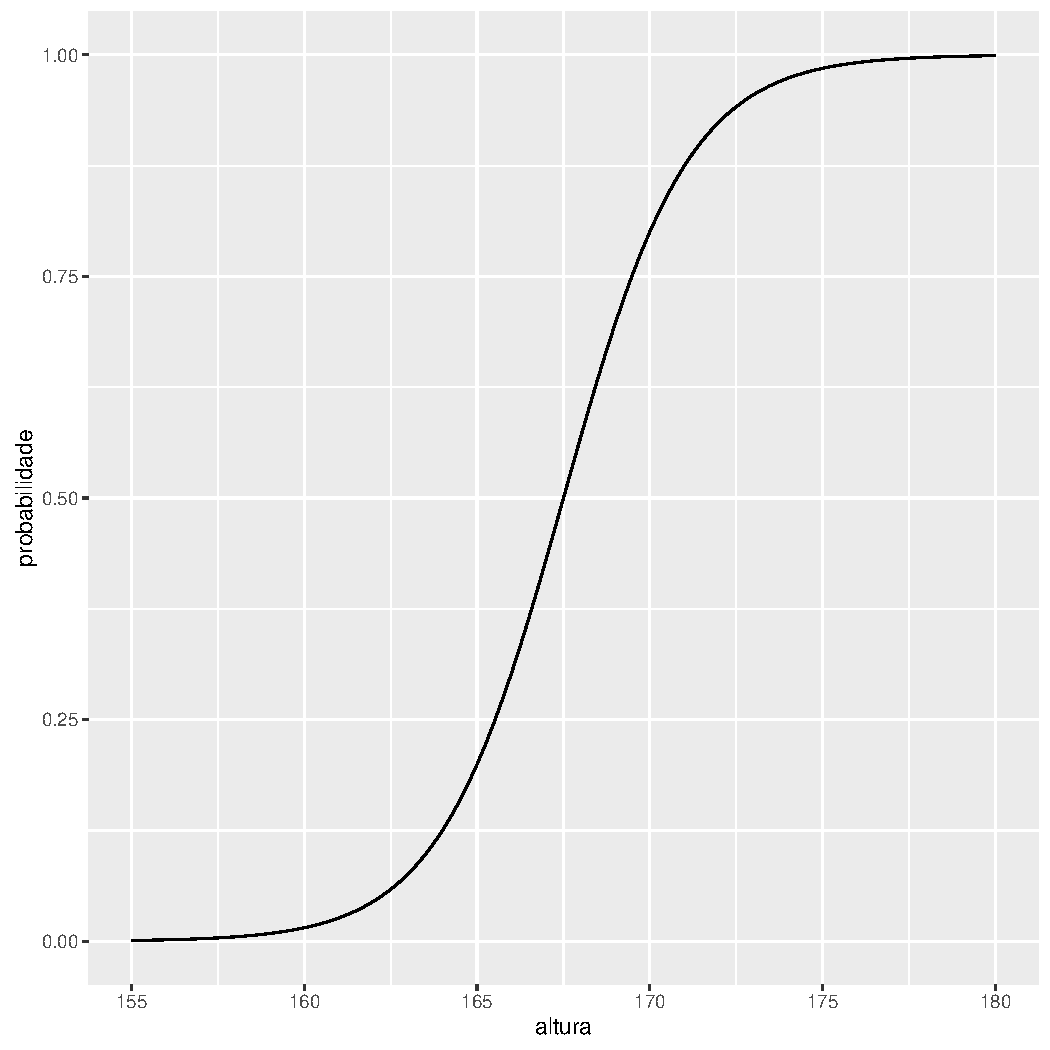
\includegraphics[scale=0.5]{chapter-revision-1-normal-mixture}
  \caption{$\P(\theta=1|X=x)$ em função de
  $x$ para o \cref{ex:normal-mixture}.}
  \label{fig:normal-mixture}
 \end{figure}
}{}

\begin{exercise}
 Considere que $\mu \in \{\mu_{1},\mu_{2}\}$,
 onde $\mu_{1}, \mu_{2} \in \mathbb{R}^{n}$ e
 $\Sigma^{2}$ é uma matriz de variância conhecida.
 Também, $X|\mu \sim N(\mu,\Sigma^{2})$ e
 $\P(\mu=\mu_{1})=0.5$.
 \begin{enumerate}[label=(\alph*)]
  \item Ache $\P(\mu=\mu_{1}|X=x)$.
  \item Mostre que
  $\{x: P(\mu=\mu_{1}|X=x) = 0.5\}$ é um hiperplano.
 \end{enumerate}
\end{exercise}

\begin{exercise}
 A proporção de deputados aliados ao governo em
 um determinado país é aproximadamente 60\%.
 Para cada projeto de lei,
 o deputado pode votar contra o projeto,
 a seu favor ou se abster da votação.
 Se um deputado é aliado ao governo,
 a probabilidade de que ele vote a favor de
 cada lei é 70\%, de que ele se abstenha é 20\% e
 de que vote contra é 10\%.
 Similarmente, se o deputado não é aliado ao governo,
 a probabilidade de que ele vote
 a favor de cada lei é 40\%, de que ele se abstenha
 é 10\% e de que vote contra é 50\%.
 Se um deputado selecionado aleatoriamente
 votou a favor de 2 projetos, se absteve de 1 projeto
 e votou contra 1 projeto,
 qual é a probabilidade de que ele seja
 aliado ao governo?
\end{exercise}

\solution{\textbf{Solução}: Defina
 \begin{align*}
  \begin{cases}
   \theta&: \text{ a indicadora de que o deputado é
   aliado ao governo, }
   \theta \in \{0,1\} \\
   X_{i}&:  \text{ o voto dado pelo deputado para
   a i-ésima proposta de lei, }
   X_{i} \in \{F,C,A\}
  \end{cases}
 \end{align*}
 Defina
 \begin{align*}
  V	&= \{X_{1}=F,X_{2}=F,X_{3}=A,X_{4}=C\}
 \end{align*}
 Assumimos que os $X_{i}$ são independentes dado
 $\theta$. Note que
 \begin{align*}
  \P(V|\theta=1)	
  &= \P(X_{1}=F,X_{2}=F,X_{3}=A,X_{4}=C|\theta=1) \\
  &=\P(X_{1}=F|\theta=1)\P(X_{2}=F|\theta=1)
  \P(X_{3}=A|\theta=1)\P(X_{4}=C|\theta=1) \\
  &= 0.7 \cdot 0.7 \cdot 0.2 \cdot 0.1 = 0.0098 \\
  \P(V|\theta=0)
  &= \P(X_{1}=F,X_{2}=F,X_{3}=A,X_{4}=C|\theta=0) \\
  &= \P(X_{1}=F|\theta=0)
  \P(X_{2}=F|\theta=0)P(X_{3}=A|\theta=0)
  \P(X_{4}=C|\theta=0) \\
  &= 0.4 \cdot 0.4 \cdot 0.1 \cdot 0.5 = 0.008
 \end{align*}
 Portanto,
 \begin{align*}
  \P(\theta=1|V)
  &= \frac{\P(\theta=1)\P(V|\theta=1)}
  {\P(\theta=1)\P(V|\theta=1)
  +\P(\theta=0)\P(V|\theta=0)} \\
  &= \frac{0.6 \cdot 0.0098}
  {0.6 \cdot 0.0098 + 0.4 \cdot 0.008} \approx 0.65
 \end{align*}
}{}

\begin{exercise}
 \label{ex:pareto-uniform}
 Considere que dado $\theta$,
 $X_{1} \ldots X_{n}$ são i.i.d. e
 $X_{i}|\theta \sim \text{Uniforme}(0,\theta)$.
 Considere que, a priori, temos que,
 para $\alpha, \beta > 0$,
 \begin{align*}
  f(\theta) = \frac{\alpha \beta^{\alpha}}
  {\theta^{\alpha+1}}\I(\theta)_{(\beta,\infty)}.
 \end{align*}
 \begin{enumerate}[label=(\alph*)]
  \item Ache a posteriori para
  $\theta|X_{1},\ldots,X_{n}$.
  Ache a forma exata da posteriori,
  não basta indicá-la até uma constante de
  proporcionalidade.
  \item Calcule $\lim_{n \rightarrow \infty}{\E[\theta|X_{1},\ldots,X_{n}]}$.
  \item Ache $f(x_{n}|x_{1},\ldots,x_{n-1})$.
  Lembre-se que esta é a distribuição preditiva, 
  que não depende de $\theta$.
 \end{enumerate}
\end{exercise}

\solution{\textbf{Solução}: 
 \begin{enumerate}[label=(\alph*)]
  \item
  \begin{align*}
   f(\theta|x_{1},\ldots,x_{n})
   &\propto f(\theta)f(x_{1},\ldots,x_{n}|\theta) \\
   &= f(\theta)\prod_{i=1}^{n}{f(x_{i}|\theta)} \\
   &= \frac{\alpha \beta^{\alpha}}
   {\theta^{\alpha+1}}\I(\theta)_{(\beta,\infty)}
   \prod_{i=1}^{n}{\theta^{-1}I(x_{i})_{(0,\theta)}}\\
   &\propto \theta^{-(\alpha+n+1)}
   \I(\theta)_{(\beta,\infty)}\prod_{i=1}^{n}
   {\I(\theta)_{(x_{i},\infty)}} \\
   &= \theta^{-(\alpha+n+1)}
   \I(\theta)_{(\beta,\infty)}
   \I(\theta)_{(x_{(n)},\infty)} \\
   &= \theta^{-(\alpha+n+1)}
   \I(\theta)_{(\max(\beta,x_{(n)}),\infty)}
  \end{align*}
  Portanto, $\theta|X_{1},\ldots,X_{n} \sim \text{Pareto}\left(\alpha+n, \beta^{*}\right)$, onde 
  $\beta^{*}=\max(\beta,x_{(n)})$.
  \item Se $\theta \sim \text{Pareto}(\alpha,\beta)$,
  então
  \begin{align*}
   \E[\theta]
   &= \int{\theta f(\theta) d\theta} \\
   &= \int{\theta \frac{\alpha \beta^{\alpha}}
   {\theta^{\alpha+1}}\I(\theta)_{(\beta,\infty)} d\theta} \\
   &= \alpha \beta^{\alpha}\int{\theta^{-\alpha}\I(\theta)_{(\beta,\infty)} d\theta} \\
   &= \frac{\alpha \beta^{\alpha}}{(\alpha-1) \beta^{\alpha-1}} = \frac{\alpha \beta}{(\alpha-1)}
   & \text{Pareto}(\alpha-1,\beta)
  \end{align*}
  Portanto,
  \begin{align*}
   \lim_{n \rightarrow \infty}
   {\E[\theta|X_{1},\ldots,X_{n}]}
   &= \lim_{n \rightarrow \infty}
   {\frac{(\alpha+n)\beta^{*}}{(\alpha+n-1)}} \\
   &= \lim_{n}\beta^{*} = \lim_{n}\max(\beta,X_{(n)})
  \end{align*}
  Note que, se $\beta$ for suficientemente pequeno,
  então $\E[\theta|X_{1},\ldots,X_{n}]$ converge
  para o estimador de máxima verossimilhança,
  $X_{(n)}$.
  \item
  \begin{align*}
   f(x_{n+1}|x_{1},\ldots,x_{n})
   &= \int_{0}^{\infty}{f(x_{n+1}|\theta)
   f(\theta|x_{1},\ldots,x_{n})d\theta}	\\
   &= \int_{0}^{\infty}{f(x_{n+1}|\theta)
   f(\theta|x_{1},\ldots,x_{n})d\theta}	\\
   &= \int_{0}^{\infty}{\theta^{-1}\I_{(0,\theta)}
   (x_{n+1}) \frac{(\alpha+n) (\beta^{*})^{\alpha+n}}
   {\theta^{\alpha+n+1}}\I(\theta)_{(\beta^{*},\infty)} d\theta} \\
   &= (\alpha+n) (\beta^{*})^{\alpha+n}\int_{0}^{\infty}{\frac{I(\theta)_{(\max(\beta^{*},x_{n+1}),\infty)}}{\theta^{\alpha+n+2}} d\theta} \\
   &= \frac{(\alpha+n) (\beta^{*})^{\alpha+n}}{(\alpha+n+1) (\max(\beta^{*},x_{n+1}))^{\alpha+n+1}}
   = \frac{(\alpha+n) (\max(\beta,x_{(n)}))^{\alpha+n}}{(\alpha+n+1) (\max(\beta,x_{(n+1)}))^{\alpha+n+1}}
  \end{align*}
  Note que, se $n$ for suficientemente grande, então
  $X_{n+1}|X_{1},\ldots,X_{n} \approx U(0,X_{(n)})$.
 \end{enumerate}
}{}

\begin{exercise}
 Considere que $\beta > 0$ é conhecido e, dado $\alpha$,
 $X_{1},\ldots,X_{n}$ são i.i.d. e $X_{1} \sim \text{Pareto}(\alpha,\beta)$.
 Ou seja, $f(x_{1}|\alpha) = \frac{\alpha \beta^{\alpha}}{x^{\alpha+1}}\I_{(\beta,\infty)}(x)$.
 \begin{enumerate}[label=(\alph*)]
  \item Mostre que $f(x_1|\alpha)$ faz parte da
  família exponencial.
  \item Se $\alpha$ fosse conhecido e
  $\beta$ desconhecido,
  $f(x_1|\beta)$ faria parte da família exponencial?
  \item Se $\alpha \sim \text{Gamma}(\gamma,\delta)$,
  identifique o nome e os hiperparâmetros da
  posteriori, $f(\alpha|x_{1},\ldots,x_{n})$.
  \item Ache $\lim_{n \rightarrow \infty} \E[\alpha|X_{1},\ldots,X_{n}]$.
  \item Ache uma família conjugada para
  $f(x_1|\alpha)$.
 \end{enumerate}
\end{exercise}

\solution{\textbf{Solução}: 
 \begin{enumerate}[label=(\alph*)]
  \item 
  \begin{align*}
   f(x_1|\alpha)
   &= \frac{\alpha \beta^{\alpha}}
   {x^{\alpha+1}}\I_{(\beta,\infty)}(x) \\
   &= \I_{(\beta,\infty)}(x) \exp\left(-(\alpha+1)\log(x) + \log(\alpha) + \alpha \log(\beta)\right)
  \end{align*}
  Portanto, $f(x_1|\alpha)$ pertence à
  família exponencial tomando
  \begin{align*}
   \begin{cases}
    h(x) &= \I_{(\beta,\infty)}(x) \\
    T(x) &= \log(x) \\
    g(\alpha) &= -(\alpha+1) \\
    A(\alpha) &= -(\log(\alpha) +\alpha \log(\beta))
   \end{cases}
  \end{align*}
  \item Se $\beta$ fosse desconhecido, então
  o suporte de $f(x_{1}|\beta)$ dependeria
  do parâmetro. Assim, $f(x_{1}|\beta)$
  não faria parte da família exponencial.
  \item
  \begin{align*}
   f(\alpha|x_{1},\ldots,x_{n})
   &\propto f(\alpha)f(x_{1},\ldots,x_{n}|\alpha) \\
   &=f(\alpha)\prod_{i=1}^{n}{f(x_{i}|\alpha)} \\
   &\propto \alpha^{\gamma-1}\exp\left(-\delta \alpha\right) \prod_{i=1}^{n}{\frac{\alpha \beta^{\alpha}}{x_{i}^{\alpha+1}}} \\
   &= \alpha^{n+\gamma-1}\exp\left(-\left(\delta+\sum_{i=1}^{n}{\log\left(\frac{x_{i}}{\beta}\right)} \right)\alpha \right)
  \end{align*}
  Portanto, $\alpha|X_{1},\ldots, X_{n} \sim \text{Gamma}\left(n+\gamma, \delta+\sum_{i=1}^{n}{\log\left(\frac{x_{i}}{\beta}\right)}\right)$.
  \item
  \begin{align*}
   \lim_{n \rightarrow \infty}
   \E[\alpha|X_{1},\ldots,X_{n}]
   &= \lim_{n \rightarrow \infty}
   \frac{n+\gamma}{\delta+\sum_{i=1}^{n}
   {\log\left(\frac{x_{i}}{\beta}\right)}} \\
   &= \lim_{n \rightarrow \infty}
   \frac{n}{\sum_{i=1}^{n}{\log\left(\frac{x_{i}}
   {\beta}\right)}}
  \end{align*}
  \item Pelo item (c), provamos que se
  a priori para $\alpha$ pertence à família Gamma,
  então a posteriori para $\alpha$ tambem
  pertence à família Gamma. Portanto,
  a família Gamma é conjugada para
  $f(x_{1}|\alpha)$.
 \end{enumerate}
}{}

%aqui
\begin{exercise}
 Considere que foram colocadas $3$ bolas em uma urna,
 sendo todas elas azuis ou verdes.
 Você está interessada em determinar o
 número de bolas azuis na urna e,
 a priori, este número pode assumir qualquer um
 dos valores possíveis com mesma probabilidade.
 Também considere que esta é uma urna de Polya,
 ou seja, a cada vez que uma bola é retirada,
 duas bolas da mesma cor da bola retirada são
 repostas na urna.
 Por exemplo, se uma urna de Polya tem
 $2$ bolas azuis e $2$ verdes
 e uma bola azul é retirada,
 então a composição passará a ser
 $3$ bolas azuis e $2$ verdes.
 Duas bolas foram retiradas da urna,
 sendo que suas cores foram, respectivamente:
 azul e azul.
 \begin{enumerate}[label=(\alph*)]
  \item Identifique os elementos do
  modelo estatístico e os valores que
  estes podem assumir.
  \item Dado cada possível valor para o parâmetro,
  calcule a covariância entre a indicadora de que a
  primeira bola retirada é azul e a
  indicadora de que a segunda é azul.
  As observações são independentes dado o parâmetro?
  \item Calcule a distribuição a posteriori para
  o parâmetro do modelo.
  \item Calcule a probabilidade preditiva de que
  a próxima bola retirada seja azul.
  \item Calcule a probabilidade marginal de
  observar os dados.
 \end{enumerate}
\end{exercise}

\solution{\textbf{Solução}:
 \begin{enumerate}[label=(\alph*)]
  \item Defina
  \begin{align*}
   \begin{cases}
    \theta&: \text{ o número de bolas azuis na urna, }
    \theta \in \{0,1,2,3\} \\
    X_{i}&: \text{ a indicadora de que a
    i-ésima bola retirada é azul, }
    X_{i} \in \{0,1\}
   \end{cases}
  \end{align*}
  \item 
  \begin{align*}
   Cov[X_{1},X_{2}|\theta=i]
   &=\E[X_{1}X_{2}|\theta=i]
   -\E[X_{1}|\theta=i]\E[X_{2}|\theta=i] \\
   &= P(X_{1}=1,X_{2}=1|\theta=i)
   -\P(X_{1}=1|\theta=i)P(X_{2}=1|\theta=i) \\
   &= \frac{i(i+1)}{12} - \frac{i^{2}}{9} \geq 0
  \end{align*}
  Em particular, se $i \in \{1,2\}$,
  $Cov[X_{1},X_{2}|\theta=i] > 0$.
  \item
  \begin{align*}
   \P(\theta=i|X_{1}=1,X_{2}=1)
   &= \frac{\P(\theta=i)P(X_{1}=1,X_{2}=1|\theta=i)}
   {\sum_{j=0}^{4}{\P(\theta=i)
   \P(X_{1}=1,X_{2}=1|\theta=i)}} \\
   &= \frac{4^{-1}\P(X_{1}=1,X_{2}=1|\theta=i)}
   {\sum_{j=0}^{4}{4^{-1}\P(X_{1}=1,X_{2}=1|\theta=i)}}\\
   &= \frac{\frac{i(i+1)}{12}}{\sum_{j=0}^{4}
   {\frac{j(j+1)}{12}}} \\
   &= \frac{i(i+1)}{\sum_{j=0}^{4}{j(j+1)}}
   =\frac{i(i+1)}{40}
  \end{align*}
  \item 
  \begin{align*}
   \P(X_{3}=1|X_{1}=1,X_{2}=1)
   &= \sum_{i=0}^{4}{\P(\theta=i|X_{1}=1,X_{2}=1)
   \P(X_{3}=1|\theta=i,X_{1}=1,X_{2}=1)} \\
   &= \sum_{i=0}^{4}{\frac{i(i+1)}{20}
   \cdot \frac{i+2}{5}} \\
   &= \sum_{i=0}^{4}{\frac{i(i+1)(i+2)}{100}} = 0.9
  \end{align*}
  
  \item
  \begin{align*}
   \P(X_{1}=1,X_{2}=1)
   &= \sum_{j=0}^{4}
   {\P(X_{1}=1,X_{2}=1|\theta=j)\P(\theta=j)} \\
   &= \sum_{j=0}^{4}{\frac{j(j+1)}{12} \cdot \frac{1}{4}}
   = \frac{20}{48}
  \end{align*}
 \end{enumerate}
}{}

\begin{exercise}
 \label{ex:simple-linear-regression}
 Considere que $Y_{i} = \theta x_{i} + \epsilon_{i}$,
 onde $\epsilon_{i}$ são i.i.d. e
 $\epsilon_{1} \sim N(0,1)$.
 Ou seja, dado $\theta$,
 $Y_{i} \sim N(\theta x_{i}, 1)$.
 Considere que, a priori,
 $\theta \sim N(0,1)$.
 \begin{enumerate}[label=(\alph*)]
  \item Ache a posteriori para
  $\theta|(x_{1},y_{1}),\ldots,(x_{n},y_{n})$.
  \item Ache $\lim_{n \rightarrow \infty}\E[\theta|(x_{1},y_{1}),\ldots,(x_{n},y_{n})]$.
 \end{enumerate}
\end{exercise}

\solution{\textbf{Solução}:
 \begin{enumerate}[label=(\alph*)]
  \item
  \begin{align*}
   f(\theta|(x_{1},y_{1}),\ldots,(x_{n},y_{n}))
   &\propto f(\theta)f((x_{1},y_{1}),\ldots,(x_{n},y_{n})|\theta) \\
   &= f(\theta)\prod_{i=1}^{n}
   {f((x_{i},y_{i})|\theta)} \\
   &\propto \exp\left(-\frac{\theta^{2}}{2}\right) \prod_{i=1}^{n}{\exp\left(-\frac{(y_{i}-x_{i}\theta)^{2}}{2}\right)}	\\
   &= \exp\left(-\frac{\theta^{2}}{2}\right) \exp\left(-\frac{\sum_{i=1}^{n}{(y_{i}-x_{i}\theta)^{2}}}{2}\right)\\
   &= \exp\left(-\frac{\theta^{2}}{2}\right) \exp\left(-\frac{\theta^{2}\sum_{i=1}^{n}{x_{i}^{2}}-2\theta\sum_{i=1}^{n}{x_{i}y_{i}}+\sum_{i=1}^{n}{y_{i}^{2}}}{2}\right) \\
   &\propto \exp\left(-\frac{\theta^{2}\left(1+\sum_{i=1}^{n}{x_{i}^{2}}\right)-2\theta\sum_{i=1}^{n}{x_{i}y_{i}}}{2}\right) \\
   &= \exp\left(-\frac{\theta^{2}-2\theta\frac{\sum_{i=1}^{n}{x_{i}y_{i}}}{\left(1+\sum_{i=1}^{n}{x_{i}^{2}}\right)}}{2\left(1+\sum_{i=1}^{n}{x_{i}^{2}}\right)^{-1}}\right) 
   \propto \exp\left(-\frac{\left(\theta-\frac{\sum_{i=1}^{n}{x_{i}y_{i}}}{\left(1+\sum_{i=1}^{n}{x_{i}^{2}}\right)}\right)^{2}}{2\left(1+\sum_{i=1}^{n}{x_{i}^{2}}\right)^{-1}}\right)
  \end{align*}
  A última passagem completa quadrados, 
  assim como no \cref{lemma:conjugate_normal_mean}.
  Note que
  \begin{align*}
   \theta|(x_{1},y_{1}),\ldots,(x_{n},y_{n}) \sim N\left(\frac{\sum_{i=1}^{n}{x_{i}y_{i}}}{\left(1+\sum_{i=1}^{n}{x_{i}^{2}}\right)}, \left(1+\sum_{i=1}^{n}{x_{i}^{2}}\right)^{-1}\right)
  \end{align*}
  \item 
  \begin{align*}
   \lim_{n \rightarrow \infty}
   \E[\theta|(x_{1},y_{1}),\ldots,(x_{n},y_{n})]
   &= \lim_{n \rightarrow \infty} \frac{\sum_{i=1}^{n}{x_{i}y_{i}}}{\left(1+\sum_{i=1}^{n}{x_{i}^{2}}\right)} \\
   & \lim_{n \rightarrow \infty} \frac{\sum_{i=1}^{n}{x_{i}y_{i}}}{\left(\sum_{i=1}^{n}{x_{i}^{2}}\right)}	\\
   &= \lim_{n \rightarrow \infty} (x^{t}x)^{-1}x^{t}y
  \end{align*}
 \end{enumerate}
}{}

\begin{exercise}
 Considere que, dado $\nu$,
 $X \sim \text{N}_{n}(\mu, \nu)$, ou seja,
 $X$ tem distribuição normal multivariada
 com média $\mu$ (conhecida) e precisão $\nu$.
 Se, a priori, $\nu \sim \text{Wishart}(V,a)$,
 ache o nome da distribuição de $\nu|X$ e
 seus hiperparâmetros.
\end{exercise}

\solution{\textbf{Solução}:
 \begin{align*}
  f(\nu|x) &\propto f(\nu)f(x|\nu) \\
  &\propto \|\nu\|^{\frac{a-p-1}{2}}\exp\left(-\frac{tr(V^{-1}\nu)}{2}\right) \|\nu\|^{\frac{1}{2}} \exp\left(-\frac{tr((x-\mu)(x-\mu)^{T}\nu)}{2}\right) \\
  &= \|\nu\|^{\frac{(a+1-p)-1}{2}}\exp\left(-\frac{tr((V^{-1}+(x-\mu)(x-\mu)^{T})\nu)}{2}\right)
 \end{align*}
 Portanto, $\nu|x \sim \text{Wishart}(a+1-p, V^{-1}+(x-\mu)(x-\mu)^{T})$.
}{}

\begin{exercise}[\citet{Gelman2014}]
 $X_{1}$ e $X_{2}$ são condicionalmente i.i.d.
 dado $\theta$. Mostre que, se $\V[\E[X_{1}|\theta]] > 0$,
 então $Cov(X_{1},X_{2}) > 0$.
\end{exercise}

\solution{\textbf{Solução}:
 \begin{align*}
  Cov[X_{1},X_{2}]
  &= \E[X_{1}X_{2}] -\E[X_{1}]\E[X_{2}] \\
  &= \E[\E[X_{1}X_{2}|\theta]]
  -\E[\E[X_{1}|\theta]]\E[\E[X_{2}|\theta]] \\
  &= \E[\E[X_{1}|\theta]\E[X_{2}|\theta]]
  -\E[\E[X_{1}|\theta]]\E[\E[X_{2}|\theta]]
  & \text{$X_{1}$ indep. $X_{2}|\theta$} \\
  &= \E[\E[X_{1}|\theta]\E[X_{1}|\theta]]
  -\E[\E[X_{1}|\theta]]\E[\E[X_{1}|\theta]]
  & \text{$X_{1}$ e $X_{2}$ i.d. dado $\theta$} \\
  &= \E[\E[X_{1}|\theta]^{2}]
  -\E[\E[X_{1}|\theta]]^{2} \\
  &= \E[\V[X_{1}|\theta]] \geq 0
 \end{align*}
}{}

\begin{exercise}
Seja $T(X)$ uma estatística suficiente para $\theta$. 
Mostre que 
$f(\theta|T=t(x))=f(\theta|X=x)$. 
Interprete esse resultado.
\end{exercise}

\newpage

\section{Tomando decisões conscientemente}
\label{section:decisions}

Você está constantemente tomando decisões.
Ir ou não ir à próxima aula de Estatística Bayesiana?
O que comer no jantar?
Trabalhar ou se divertir?
Se você pensar com cuidado, 
geralmente será capaz de identificar
diversas alternativas para cada uma
de suas ações.
A sua ação foi uma decisão
dentre todas as alternativas possíveis.

Mesmo assim, apesar de sua ação ter alternativas,
você nem sempre pensa conscientemente sobre
qual será sua decisão.
Seja por falta de tempo,
seja por não conhecer outra forma de fazê-lo,
muitas vezes você toma decisões intuitivamente,
alheia aos motivos que tornam a sua escolha
melhor ou pior do que as alternativas.

Contudo, nossa intuição
muitas vezes não passaria por
uma inspeção mais cuidadosa.
Por exemplo, considere a decisão entre
comer ou não comer uma barra de chocolate.
Nós evoluímos de macacos
em uma guerra permanente para sobreviver à fome.
Destes mesmos macacos 
herdamos o impulso de avançar sobre
a barra de chocolate e comê-la inteira.
Contudo, a nossa situação é consideravelmente
diferente da dos macacos.
Temos maneiras seguras de reservar alimentos
e ingerí-los mais tarde.
Para muitos humanos,
a guerra não é mais sobreviver à fome,
mas sim à obesidade.
Portanto, ainda que nosso primeiro impulso seja
comer a barra de chocolate inteira,
em muitas situações é possível elaborar argumentos
que justificariam reservar parte ou a totalidade da
barra de chocolate para ser comida mais tarde.
Pensando com cuidado, 
às vezes você concluirá que a melhor decisão para você
será diferente de sua intuição inicial.

Neste Capítulo você estudará um processo consciente
de tomada de decisões.
Chamaremos este processo de Teoria da Decisão.
A Teoria da Decisão é dividida em etapas,
que indicam questões relevantes na tomada de qualquer decisão.
Quando você completar todas as etapas indicadas,
a Teoria da Decisão sugerirá
qual ação é a mais proveitosa para você.

\subsection{Elementos da tomada de decisões}
\label{section:decisions_elements}

A Teoria da decisão lhe indicará qual é a melhor ação
dentre aquelas que você tem disponíveis.
Para tal, você terá de especificar determinados elementos,
detalhados a seguir.

Denotaremos por $\mathcal{A}$ o conjunto de ações ou alternativas
que você tem disponíveis.
Essas alternativas deverão ser expressas de tal forma que sejam mutuamente exclusivas,
ou seja, você somente poderá escolher uma única alternativa.
Contudo, esta não é uma grande limitação.
Por exemplo, se você pensar em alternativas $A$ e $B$ que não sejam mutuamente exclusivas,
poderá obter ``$A \text{ e } B$'',
``$A \text{ e não } B$'' ,
``$\text{não } A \text{ e } B$'', e
``$\text{não } A \text{ e não } B$''
como alternativas mutuamente exclusivas. Por exemplo, 
considere que você pode levar um guarda-chuva e 
uma calculadora à aula de Estatística Bayesiana.
Ainda que ``levar o guarda-chuva'' e ``levar a calculadora''
não sejam alternativas mutuamente exclusivas,
``levar o guarda-chuva e levar a calculadora'',
``levar o guarda-chuva e não levar a calculadora'',
``não levar o guarda-chuva e levar a calculadora'', e
``não levar o guarda-chuva e não levar a calculadora'' o são.
Sucintamente, denotaremos as alternativas neste exemplo por
$\mathcal{A} = \{(gc,ca), (gc,\bar{ca}), (\bar{gc},ca), (\bar{gc},\bar{ca})\}$.

É importante que você inclua em $\mathcal{A}$
todas as alternativas relevantes.
Se você esquecer de incluir a melhor decisão,
então o procedimento descrito neste Capítulo
não será capaz de indicá-la como sendo a melhor decisão.
De fato, muitas vezes o segredo do protagonista de uma história de sucesso
foi a capacidade deste de considerar uma alternativa que outros não consideraram.
A Teoria da Decisão não
enuncia diretamente qual é $\mathcal{A}$,
mas reforça a importância de conscientemente analisar com cuidado este aspecto.

Denotamos por $\Theta$ o conjunto de possíveis ocorrências
que são relevantes para a tomada da sua decisão.
Similarmente às alternativas possíveis,
as possibilidades também devem ser
mutuamente exclusivas e exaustivas. 
Por exemplo, no caso em que você decide sobre levar o
guarda-chuva e a calculadora,
uma variável importante pode ser a
ocorrência de chuva no dia.
Não queremos molhar a calculadora, mas por outro lado levar o guarda-chuva quando não chove também não é agradável.
Assim,  $\Theta$ poderia ser
o conjunto com os elementos ``chove no dia'', e 
``não chove no dia''. Denotaremos as
possibilidades neste exemplo por
$\Theta = \{ch, \bar{ch}\}$.

Associaremos uma medida de probabilidade, $\P$, a $\Theta$.
Esta medida indica a plausibilidade que você atribui a cada
elemento de $\Theta$ no momento da tomada da decisão.
Note que, caso você tenha observado dados antes
de tomar a sua decisão, então
$\P$ será a probabilidade condicionada aos dados,
a posteriori.
Suponhamos que você confia no relato metereológico, 
segundo o qual a probabilidade de chuva é de 10\%.
Assim, você obteria 
$\P(\{ch\})=10\%$ e $\P(\{\bar{ch}\})=90\%$.

Finalmente, você atribuirá uma utilidade para
cada par composto por uma alternativa,
$a \in \mathcal{A}$ e uma possibilidade,
$\theta_{0} \in \Theta$.
Esta utilidade representa o quão é
desejável para você obter a possibilidade
$\theta_{0}$ quando você escolheu $a$.
A utilidade é representada por uma função, 
$U: \mathcal{A} \times \Theta \rightarrow \mathbb{R}$,
sendo que $U(a,\theta_{0})$, indica a utilidade da
ocorrência $\theta_{0}$ tendo decidido por $a$.
Por exemplo, considere que seu par predileto é
aquele em que você leva a calculadora e
não leva o guarda-chuva em um dia sem chuva.
Também, considere que seu par menos desejado é
aquele em que você leva a calculadora e
não leva o guarda-chuva em um dia com chuva.
Para simplicidade, considere que a utilidade do
seu par favorito é $1$ e
a do seu par menos desejado é $0$.
Assim, para cada um dos demais pares, 
a utilidade será um número entre $0$ e $1$.
Neste caso, se a sua utilidade para um
determinado par é $p$, então
obter este par será tão desejável quanto
obter o melhor par com probabilidade $p$
e o pior par com probabilidade $(1-p)$.
Quando $\mathcal{A}$ e $\Theta$ são conjuntos finitos,
$U$ pode ser representado como uma tabela.
A \cref{table:utilidade} ilustra a utilidade no
exemplo envolvendo a chuva, o guarda-chuva e
a calculadora.

\begin{table}
 \centering
 \begin{tabular}{|c|c|c|}
  \hline
  $\mathcal{A} \backslash \Theta$	& $ch$ & $\bar{ch}$ \\
  \hline
  $(gc, ca)$ &	0.5 & 0.9 \\
  $(gc, \bar{ca})$ & 0.6 & 0.7 \\
  $(\bar{gc}, ca)$ & 0 & 1 \\
  $(\bar{gc}, \bar{ca})$ & 0.1 & 0.8 \\
  \hline
 \end{tabular}
 \caption{Utilidade para cada combinação de
 alternativa em $\mathcal{A}$ e
 possibilidade em $\Theta$.}
 \label{table:utilidade}
\end{table}

\begin{definition}
 Os elementos de um problema de decisão são:
 \begin{itemize}
  \item $\mathcal{A}$: o conjunto das
  alternativas disponíveis.
  Você deve escolher exatamente uma destas alternativas.
  \item $\Theta$: o conjunto de possibilidades que
  podem ocorrer. Você não escolhe qual
  destas possibilidades ocorrerá.
  \item $P$: uma medida de probabilidade sobre $\Theta$.
  Uma medida do quão plausível é
  cada possibilidade em $\Theta$.
  \item $U$: uma função de $\mathcal{A} \times \Theta$ a
  $\mathbb{R}$ que indica a utilidade de cada par.
 \end{itemize}
\end{definition}

\subsection{Avaliando alternativas}

Na \cref{table:utilidade} você encontrará a
utilidade para cada alternativa e possibilidade em
um exemplo. Observe que o par favorito é
$(\bar{gc},ca)$ e $\bar{ch}$, ou seja,
não trazer o guarda-chuva e trazer a calculadora quando
não há chuva.
Assim, se você pudesse garantir que não haveria chuva,
sua satisfação máxima seria obtida não trazendo o guarda-chuva e trazendo a calculadora.
Contudo, em geral, não é possível ter certeza sobre qual possibilidade em $\Theta$ ocorrerá.
Assim, é necessário avaliar qual a alternativa em $\mathcal{A}$ que é mais desejável 
sem fixar a possibilidade em $\Theta$ que ocorrerá.

A Teoria da decisão fornece uma forma de avaliar a utilidade de uma decisão.

\begin{definition}
 \label{defn:expected_utility}
 Considere que, para cada $a \in \mathcal{A}$,
 $U_{a}:\Theta \rightarrow \mathbb{R}$ é uma variável aleatória tal que
 $U_{a}(\theta) = U(a,\theta)$. A utilidade de uma alternativa, $a \in \mathcal{A}$, é $\E[U_{a}]$.
\end{definition}

A \cref{defn:expected_utility} permite que
você avalie a utilidade de cada
alternativa disponível sem fixar qual
possibilidade em $\Theta$ ocorrerá.
Assim, para achar qual a melhor alternativa,
basta calcular a utilidade de cada uma delas e escolher
aquela que atinge a maior utilidade.
A melhor alternativa é chamada de \emph{alternativa de Bayes}.

\begin{example}
 \label{example:decision}
 Considere o Exemplo da seção anterior.
 Podemos calcular a utilidade de cada
 alternativa em $\mathcal{A}$
 usando a \cref{defn:expected_utility}.
 \begin{align*}
  \begin{cases}
   U_{(gc,ca)} &= \P(\{ch\})U((gc,ca), ch) + \P(\bar{ch})U((gc,ca), \bar{ch}) = 0.1 \cdot 0.5 + 0.9 \cdot 0.9 = 0.86 \\
   U_{(gc,\bar{ca})} &= \P(\{ch\})U((gc,\bar{ca}), ch) + \P(\bar{ch})U((gc,\bar{ca}), \bar{ch}) = 0.1 \cdot 0.6 + 0.9 \cdot 0.7 = 0.69 \\
   U_{(\bar{gc},ca)} &= \P(\{ch\})U((\bar{gc},ca), ch) + \P(\bar{ch})U((\bar{gc},ca), \bar{ch}) = 0 \cdot 0.1 + 1 \cdot 0.9 = 0.9 \\
   U_{(\bar{gc},\bar{ca})}	&= \P(\{ch\})U((\bar{gc},\bar{ca}), ch) + \P(\bar{ch})U((\bar{gc},\bar{ca}), \bar{ch}) = 0.1 \cdot 0.1 + 0.9 \cdot 0.8 = 0.73
  \end{cases}
 \end{align*}
 Portanto, no cenário descrito, a melhor decisão é
 não levar o guarda-chuva e levar a calculadora. 
\end{example}

Em outros livros \citep{deGroot2005}, 
a \cref{defn:expected_utility} não é apresentada como
uma definição.
É possível obtê-la como um teorema a partir de
outras propriedades
mais elementares envolvendo utilidade.
Esta técnica é similar àquela que aplicamos para
obter os axiomas da probabilidade a partir de 
propriedades sobre apostas.
Para efeitos deste curso, tomaremos a \cref{defn:expected_utility}
como um ponto de partida,
deixando investigações sobre a
sua razoabilidade por sua conta.

\subsubsection*{Exercícios}

\begin{exercise}
 Modele o problema de decisão na
 situação do guarda-chuva, calculadora e chuva
 usando a sua própria probabilidade e utilidade.
 Qual a decisão ótima para você?
\end{exercise}

\begin{exercise}
 \label{ex:umbrella}
 Considere que, no \cref{example:decision}, 
 $\P(\{ch\})=p$.
 Para cada $p \in [0,1]$,
 encontre a decisão ótima.
\end{exercise}

\solution{\textbf{Solução}:
 Neste caso, teríamos,
 \begin{align}
  \label{eqn:umbrella_1}
  \begin{cases}
   U_{(gc,ca)} &= 0.5p + 0.9(1-p) \\
   U_{(gc,\bar{ca})} &= 0.6p + 0.7(1-p)	\\
   U_{(\bar{gc},ca)} &= (1-p) \\
   U_{(\bar{gc},\bar{ca})}	&= 0.1p + 0.8(1-p)
  \end{cases}
 \end{align}
 \begin{figure}
  \centering
  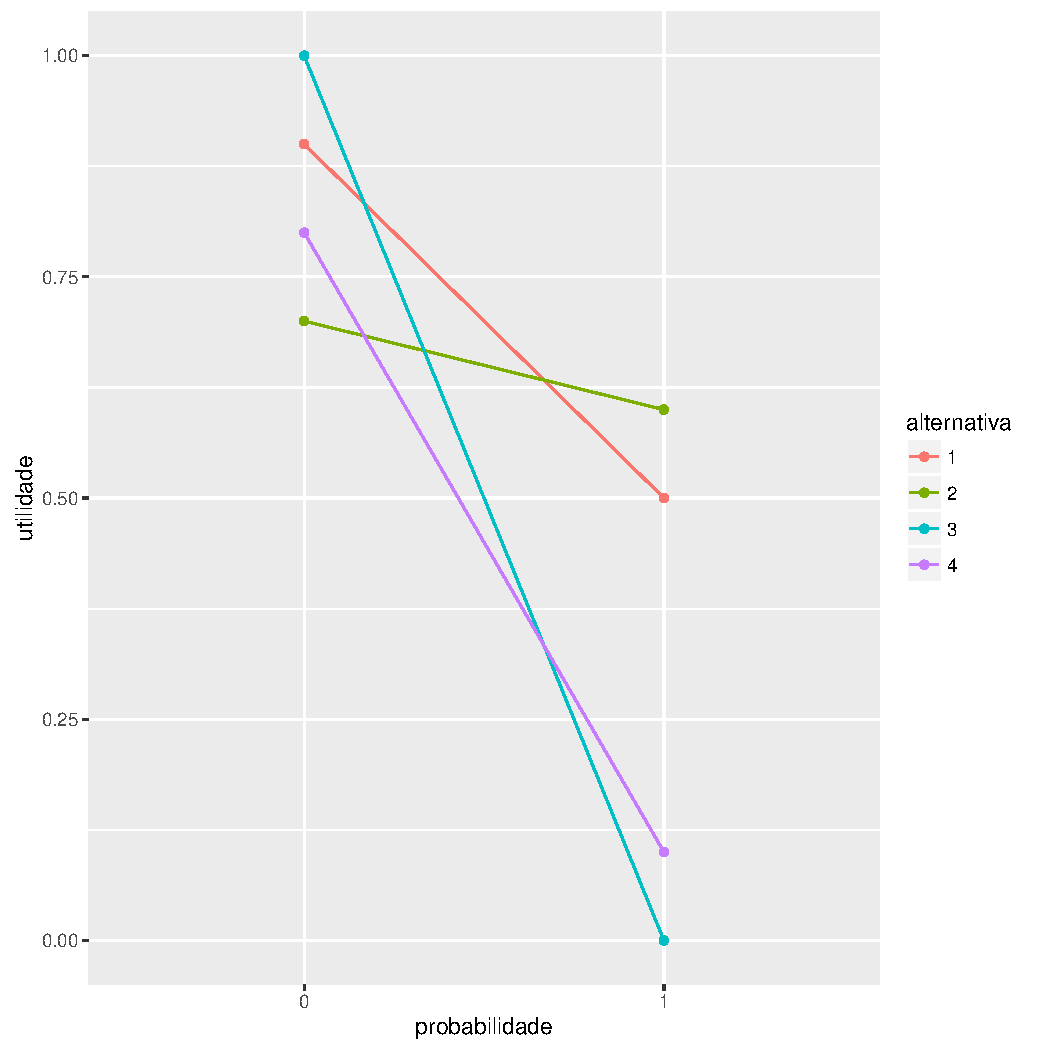
\includegraphics[scale=0.5]{chapter-decisions-umbrella.pdf}
  \caption{Utilidade esperada de cada alternativa no
  \cref{ex:umbrella} em função da probabilidade de chuva.
  As alternativas são: $1-(gc,ca)$, $2-(gc,\bar{ca})$,
  $3-(\bar{c},ca)$, $4-(\bar{gc},\bar{ca})$.}
  \label{fig:umbrella}
 \end{figure}
 Observe que a utilidade para cada uma das decisões é
 uma função linear de $p$.
 Podemos utilizar o $R$ para visualizar estas funções.
 A figura \ref{fig:umbrella} apresenta a
 utilidade esperada de cada uma
 das alternativas em função de $p$.
 A reta que está acima de todas as demais progride com
 o valor de $p$ de
 $3-(\bar{gc},ca)$, para $1-(gc,ca)$ e, finalmente,
 para $2-(gc,\bar{ca})$.
 Assim, se chuva é um evento improvável, a melhor opção é
 não trazer o guarda-chuva e trazer a calculadora.
 Quando chuva passa a ser um evento sobre
 o qual existe mais incerteza,
 a opção mais moderada, trazer o guarda-chuva e
 a calculadora, passa a ser a melhor.
 Finalmente, quando existe uma
 probabilidade suficientemente grande de que
 vai haver chuva, a melhor alternativa sob esta condição,
 levar o guarda-chuva e não a calculadora,
 passa a ser aquela com maior utilidade esperada.
 Também note que a reta $1$ está sempre acima da reta $4$.
 Em outras palavras, levar o guarda-chuva e a calculadora
 é sempre melhor do que  não levar ambos,
 não importa qual a ocorrência em $\Theta$.

 Após a inspeção gráfica, podemos determinar exatamente
 qual a melhor alternativa em $\mathcal{A}$ em
 função do valor de $p$.
 Note que a melhor opção é aquela que corresponde à
 reta acima de todas as outras.
 Assim, se $p$ está entre $0$ até o ponto em que a reta
 $3$ encontra a reta $1$, a reta $3$ é a melhor opção.
 O ponto de encontro das retas pode ser encontrado tomando
 $U_{(\bar{gc},ca)} = U_{(gc,ca)}$.
 A partir da \cref{eqn:umbrella_1},
 este valor de $p$ é encontrado resolvendo
 \begin{align*}
  1-p &= 0.5p + 0.9(1-p) \\
  p = \frac{1}{6}
 \end{align*}
 Assim, se $p \in \left[0,\frac{1}{6}\right)$, 
 a melhor alternativa é $(\bar{gc},ca)$.
 Também, se $p=\frac{1}{6}$, 
 as duas melhores opções (empatadas)
 são $(\bar{gc},ca)$ e $(gc,ca)$.
 Observamos que, a partir de $p=\frac{1}{6}$,
 a melhor alternativa é $(gc,ca)$ até o ponto
 em que a reta $1$ encontra a reta $2$.
 Este ponto pode ser encontrado tomando
 $U_{(gc,ca)} = U_{(gc,\bar{ca})}$.
 A partir da Equação \ref{eqn:umbrella_1},
 este valor de $p$ é encontrado resolvendo
 \begin{align*}
  0.5p + 0.9(1-p) &= 0.6p + 0.7(1-p) \\
  p = \frac{2}{3}
 \end{align*}
 Portanto, se
 $p \in \left(\frac{1}{6}, \frac{2}{3}\right)$,
 a melhor alternativa é $(gc, ca)$.
 Também, se $p=\frac{2}{3}$ as
 melhores alternativas (empatadas) são
 $(gc,ca)$ e $(gc,\bar{ca})$.
 Finalmente, se $p \in \left(\frac{2}{3},1\right]$,
 então a melhor alternativa é $(gc,\bar{ca})$.
 A melhor alternativa para cada possível valor de
 $p$ é resumida na \cref{table:umbrella}.
 \begin{table}
  \centering
  \begin{tabular}{|c|c|c|c|c|c|}
   \hline
   $p \in$
   & $\left[0,\frac{1}{6}\right)$
   & $\left\{\frac{1}{6}\right\}$
   & $\left(\frac{1}{6},\frac{2}{3}\right)$
   & $\left\{\frac{2}{3}\right\}$
   & $\left(\frac{2}{3},1\right]$ \\
   \hline
   $a^{*}$ & $(\bar{gc},ca)$
   & $(\bar{gc},ca)$ ou $(gc,ca)$
   & $(gc,ca)$
   & $(gc,ca)$ ou $(gc,\bar{ca})$
   & $(gc,\bar{ca})$ \\
   \hline
  \end{tabular}
  \caption{A melhor alternativa, $a^{*} \in \mathcal{A}$,
  para cada valor de $p$ no \cref{ex:umbrella}.}
  \label{table:umbrella}
 \end{table}
}{}

\begin{exercise}
 Considere que $\theta \sim \text{Bernoulli}(0.5)$.
 Suas alternativas são escolher um número real em $[0,1]$.
 Seja $a$ a sua decisão, sua utilidade é
 $-(a-\theta)^{2}$. Ou seja, quanto mais próximo de
 $\theta$, melhor será sua escolha.
 \begin{enumerate}[label=(\alph*)]
  \item Indique os elementos do problema de decisão.
  \item Ache a decisão ótima.
  \item Se o parâmetro da Bernoulli fosse $p$ ao
  invés de $0.5$, qual seria a decisão ótima?
  \item No caso acima,
  se sua utilidade fosse $-|a-\theta|$,
  qual seria a decisão ótima?
  \item Interprete o resultado anterior.
 \end{enumerate}
\end{exercise}

\solution{\textbf{Solução}:
 \begin{enumerate}[label=(\alph*)]
  \item
  \begin{align*}
   \begin{cases}
    \mathcal{A} = [0,1]
    &: \text{os números dentre os quais você
    pode escolher.} \\
    \Theta = \{0,1\}
    &: \text{os possíveis valores de $\theta$.} \\
    \P(\theta=0)=\P(\theta=1)=0.5 \\
    U(a,\theta) = -(a-\theta)^{2}
   \end{cases}
  \end{align*}
  \item Para cada a $\in [0,1]$,
  \begin{align*}
   \E[U_{a}]
   &=\P(\theta=0)U(a,0) +\P(\theta=1)U(a,1) \\
   &= 0.5 \cdot -(a-0)^{2} + 0.5 \cdot -(a-1)^{2} \\
   & =-a^{2} + a -0.5
  \end{align*}
  Esta equação do $2^{o}$ grau é
  maximizada no ponto $a^{*}=0.5$.
  Portanto, a alternativa com a maior
  utilidade esperada é $0.5$
  e, segundo, a \cref{defn:expected_utility}, 
  esta é a melhor alternativa.
  \item Similarmente ao caso anterior,
  para cada valor de $p$ e $a$, obtemos
  \begin{align*}
   \E[U_{a}]
   &=\P(\theta=0)U(a,0) +\P(\theta=1)U(a,1) \\
   &= (1-p) \cdot -(a-0)^{2} + p \cdot -(a-1)^{2} \\
   &= -a^{2} + 2pa -p
  \end{align*}
  Portanto, a decisão que maximiza a utilidade 
  esperada é $a=p$. Segundo a
  \cref{defn:expected_utility}, esta é
  a melhor decisão.
 
  Alternativamente, observe que
  \begin{align*}
   \E[U_{a}] &= \E[-(\theta-a)^{2}] \\
   &= -\V[\theta-a] -(\E[\theta]-a)^{2}	\\
   &= -\V[\theta] -(\E[\theta]-a)^{2}
  \end{align*}
  Como $\V[\theta]$ é uma constante (em $a$),
  a decisão que maximiza a utilidade esperada é
  aquela que maximiza $-(\E[\theta]-a)^{2}$, ou seja
  $\E[\theta]=p$.
  \item Neste caso, temos
  \begin{align*}
   \E[U_{a}] &= \E[-|\theta-a|] \\
   &= -|0-a|\P(\theta=0) -|1-a|\P(\theta=1) \\
   &= -a(1-p) + (-1+a)p \\
   &= a(2p-1)-p 
  \end{align*}
  Note que $\E[U_{a}]$ é uma reta em função de $a$.
  Se $2p-1$ for positivo, ou seja $p > \frac{1}{2}$,
  então esta reta é crescente e é maximizada em $a=1$.
  Se $2p-1$ for negativo, ou seja, $p < \frac{1}{2}$,
  então esta reta é decrescente e é maximizada em $a=0$.
  Finalmente, a reta é constante em $-p$ e
  todas as alternativas são igualmente desejáveis.
  Assim, se $p < \frac{1}{2}$, a melhor alternativa é $0$,
  se $p = \frac{1}{2}$, todas as alternativas são
  igualmente desejáveis e,
  se $p > \frac{1}{2}$ a melhor alternativa é $1$.
 \end{enumerate}
}{}

\begin{exercise}[\citep{Hacking1972}]
 Em um dos primeiros usos documentados da
 Teoria da Decisão, Blaise Pascal argumentou sobre o
 porquê uma pessoa deve acreditar em Deus.
 Segundo Pascal, caso Deus exista e você acredite nele,
 sua recompensa será infinita.
 Similarmente, Pascal argumenta que, 
 se Deus existe e você não acredita nele,
 sua punição será infinita.
 Finalmente, Pascal completa que,
 caso Deus não exista,
 sua utilidade será finita.
 Destas premissas Pascal argumenta que,
 por menor que seja a plausibilidade da existência de Deus,
 sua melhor alternativa é acreditar nele.
 \begin{enumerate}[label=(\alph*)]
  \item Identifique os elementos de um
  problema de decisão na aposta de Pascal.
  \item Acompanhe o argumento de Pascal.
  Supondo que suas premissas sejam verdadeiras,
  a sua conclusão está de acordo com a
  Teoria da Decisão?
  \item Você acha que as premissas de Pascal
  são razoáveis?
 \end{enumerate}
\end{exercise}

\begin{exercise}[\citet{Kadane2011}][p.290]
 Considere que você tem $R\$kx$.
 Sua utilidade para ter $R\$f$ é $\log(f)$.
 O custo de uma aposta em $A$ é $x$.
 Se você comprar a aposta,
 caso $A$ ocorra, você ganha $R\$1$ e,
 caso $A$ não ocorra, você ganha $R\$0$.
 Você acredita que $P(A) = p$.
 Se você pode comprar quantas unidades da
 aposta você quiser, qual valor
 lhe traria maior satisfação?
\end{exercise}

\begin{exercise}[\citet{Kadane2011}][p.275]
 Considere que você deve decidir entre
 participar ou não de uma aposta.
 Para participar da aposta, 
 você deve pagar $R\$a$.
 A seguir, uma moeda honesta é lançada até a
 primeira ocorrência de cara. Seja $X$ o
 número de lançamentos da moeda,
 sua recompensa é $R\$2^{X}$.
 Considere que sua utilidade é o seu ganho monetário,
 caso você participe da aposta, e $0$, caso contrário.
 \begin{enumerate}[label=(\alph*)]
  \item Qual é o maior valor de $R\$a$ tal que
  a melhor opção é participar da aposta?
  \item A conclusão acima é razoável?
  Você concorda com todos os elementos
  do problema de decisão descritos no problema?
  \item Como a sua resposta para o item (a) seria
  alterada caso sua utilidade para
  um ganho monetário, $m$, seja
  \begin{align*}
   U(m)	&=
   \begin{cases}
    \log(m) & \text{, se $m > 0$} \\
    0 & \text{, se $m = 0$} \\
    -\log(-m) & \text{, se $m < 0$}
   \end{cases}
  \end{align*}
 \end{enumerate}
\end{exercise}

\subsection{Usando dados para avaliar alternativas}

Na \cref{section:decisions_elements},
analisamos os elementos de um problema de decisão.
Em todos os exemplos que estudamos nesta seção,
uma decisão era tomada sem consultar dados.
Em outras palavras, a decisão era tomada utilizando
apenas a informação que era conhecida \emph{a priori}
a respeito de $\theta$.

Agora estudaremos o problema de tomada de
decisões  a partir de dados.
Veremos que este tipo de problema
pode ser tratado igualmente a
um problema de decisão sem dados.
Assim, as conclusões obtidas nas seções anteriores
ainda serão válidas neste tipo de problema.
Iniciamos nossa análise definindo os elementos de um 
problema de decisão com dados.

\begin{itemize}
 \item $X \in \chi$: uma quantidade desconhecida que
 expressa os dados que serão observados.
 Os dados assumem valores em $\chi$.
 \item $\theta \in \Theta$: uma quantidade desconhecida
 que é relevante para a tomada de decisões.
 \item $\P$: uma medida de probabilidade conjunta sobre
 $(X,\theta)$.
 \item $\mathcal{A}$: o conjunto de
 alternativas disponíveis para o tomador de decisão.
 No caso de um problema de decisão com dados, as
 alternativas são funções que, para cada
 dado observado, indicam qual decisão será tomada.
 Mais formalmente, existe um conjunto de
 alternativas simples, $\mathcal{A}_{*}$,
 e $\mathcal{A} = \{f(x): \chi \rightarrow \mathcal{A}_{*}\}$.
 \item $U: \mathcal{A}_{*} \times \Theta \rightarrow \mathbb{R}$:
 a utilidade de cada alternativa em $\mathcal{A}_{*}$
 combinada a cada possibilidade em $\Theta$.
\end{itemize}

\begin{example}
 \label{ex:guarda-chuva-dados}
 Todo dia antes de sair de casa,
 eu decido se colocarei meu guarda-chuva em minha mochila.
 A princípio, eu acho que a
 probabilidade de chuva é de 20\%.
 Contudo, antes de tomar uma decisão,
 eu consulto a previsão do tempo.
 Eu acredito que a probabilidade de a
 previsão do tempo estar correta é de 90\%.
 Caso não chova e eu não leve meu guarda-chuva,
 eu ficarei maximamente satisfeito, 
 atribuindo utilidade $1$ a esse resultado.
 Caso chova e eu não leve meu guarda-chuva,
 eu ficarei minimamente satisfeito, 
 atribuindo utilidade $0$ a esse resultado.
 Caso chova e eu leve meu guarda-chuva, 
 a utilidade será $0.6$.
 Finalmente, caso não chova e 
 eu leve meu guarda-chuva, 
 a utilidade é $0.9$.

 Posso traduzir a descrição acima em 
 um problema de decisão com dados:
 \begin{itemize}
  \item $X \in \{0,1\}:$ 
  a indicadora de que há uma previsão de chuva.
  \item $\theta \in \{0,1\}:$ 
  a indicadora de ocorrência de chuva no dia.
  \item $P$: a função de probabilidade conjunta de
  $(\theta,X)$ obtida da seguinte forma:
  \begin{align*}
   \begin{cases}
    \P(\theta=0,X=0)	
    &= \P(\theta=0)\P(X=0|\theta=0)
    = 0.8 \cdot 0.9 = 0.74 \\
	\P(\theta=0,X=1)	
    &= \P(\theta=0)\P(X=1|\theta=0) 
    = 0.8 \cdot 0.1 = 0.08 \\
	\P(\theta=1,X=0)	
    &= \P(\theta=1)\P(X=0|\theta=1) 
    = 0.2 \cdot 0.1 = 0.02 \\
	P(\theta=1,X=1)	
    &= \P(\theta=1)\P(X=1|\theta=1) 
    = 0.2 \cdot 0.9 = 0.18
   \end{cases}
  \end{align*}
  \item $\mathcal{A}$: 
  O conjunto de funções que 
  tomam a decisão de levar ou 
  não levar o guarda-chuva para
  cada possível previsão do tempo.
  Denote ``levar o guarda-chuva'' por ``$g$'' e
  ``não levar o guarda-chuva'' por ``$\bar{g}$''.
  Como existem $2$ previsões possíveis e 
  2 decisões para cada previsão,
  existe um total de $4$ destas funções.
  Mais precisamente, $\mathcal{A} = \{\delta: \{0,1\} \rightarrow \{g,\bar{g}\}\}$.
  O conjunto de alternativas é descrito 
  na tabela \ref{ex:chuva-dados}.
  Estas alternativas podem ser interpretadas 
  em linguagem comum.
										
  $\delta_{1}$ nunca leva o guarda-chuva.
										
  $\delta_{2}$ leva o guarda-chuva se 
  é previsto chuva e não leva, caso contrário.
  
  $\delta_{3}$ leva o guarda-chuva se é previsto
  não haver chuva e não leva, caso contrário.
  
  $\delta_{4}$ sempre leva o guarda-chuva.
  \begin{table}
   \centering
   \begin{tabular}{|c|l|l|}
    \hline
    alternativa & $X=0$ & $X=1$ \\
	\hline
	$\delta_{1}$ & $\bar{g}$ & $\bar{g}$ \\
	$\delta_{2}$ & $\bar{g}$ & $g$ \\
	$\delta_{3}$ & $g$ & $\bar{g}$ \\
	$\delta_{4}$ & $g$ & $g$ \\
	\hline
   \end{tabular}
   \caption{Descrição de cada alternativa em
   $\mathcal{A}$, ou seja,
   $\delta_{1}, \delta_{2}, \delta_{3}$ e 
   $\delta_{4}$. Cada alternativa é 
   descrita indicando a decisão simples que
   é tomada para cada possível valor 
   observado de $X$.}
   \label{ex:chuva-dados}
  \end{table}
  \item $U(0,0) = 1$, 
  $U(0,1) = 0$, $U(1,0) = 0.9$, $U(1,1) = 0.6$.	 
 \end{itemize}
\end{example}

Os elementos de um problema de decisão com dados
são semelhantes àqueles existentes em um problema de decisão sem dados.
As únicas diferenças são a adição de um novo elemento
representando os dados, $X$, e 
a extensão da probabilidade para também incluir os dados.
Assim, no contexto em que temos dados,
a melhor alternativa ainda é aquela que
apresenta a melhor utilidade esperada.

\begin{example}[Continuação do \cref{ex:guarda-chuva-dados}]
 \label{ex:guarda-chuva-dados-2}
 Existem quatro alternativas em $\mathcal{A}$,
 conforme descrito na tabela \ref{ex:chuva-dados}.
 Assim, para determinar qual a melhor delas,
 podemos calcular a utilidade esperada de cada uma delas.
 \begin{align*}
  \E[U_{\delta_{i}}]
  &= \E[U(\delta_{i}(X),\theta)] \\
  &= \sum_{\theta_{0}=0}^{1}{\sum_{x=0}^{1}{U(\delta_{i}(x),\theta_{0})P(\theta=\theta_{0},X=x)}} \\
 \end{align*}
 \begin{align*}
  \E[U_{\delta_{1}}]
  =& U(\delta_{1}(0),0)\P(\theta=0,X=0)
  +U(\delta_{1}(0),1)\P(\theta=0,X=1) +	\\
  & U(\delta_{1}(1),0)\P(\theta=1,X=0)
  + U(\delta_{1}(1),1)\P(\theta=1,X=1) \\
  =& U(\bar{g},0)\P(\theta=0,X=0)+ 
  U(\bar{g},0)\P(\theta=0,X=1) + \\
  & U(\bar{g},1)\P(\theta=1,X=0) +
  U(\bar{g},1)\P(\theta=1,X=1) \\
  =& 1 \cdot 0.72 + 1 \cdot 0.08
  + 0 \cdot 0.02 + 0 \cdot 0.18 = 0.8
 \end{align*}
 \begin{align*}
  \E[U_{\delta_{2}}]
  =& U(\delta_{2}(0),0)\P(\theta=0,X=0)
  + U(\delta_{2}(0),1)\P(\theta=0,X=1) + \\
  & U(\delta_{2}(1),0)\P(\theta=1,X=0) +
  U(\delta_{2}(1),1)\P(\theta=1,X=1) \\
  =& U(\bar{g},0)\P(\theta=0,X=0)
  + U(g,0)\P(\theta=0,X=1) + \\
  & U(\bar{g},1)\P(\theta=1,X=0) +
  U(g,1)\P(\theta=1,X=1) \\
  =& 1 \cdot 0.72 + 0.9 \cdot 0.08
  + 0 \cdot 0.02 + 0.6 \cdot 0.18 = 0.9
 \end{align*}
 \begin{align*}
  \E[U_{\delta_{3}}]
  =& U(\delta_{3}(0),0)\P(\theta=0,X=0)
  + U(\delta_{3}(0),1)\P(\theta=0,X=1) + \\
  & U(\delta_{3}(1),0)\P(\theta=1,X=0) +
  U(\delta_{3}(1),1)\P(\theta=1,X=1) \\
  =& U(g,0)\P(\theta=0,X=0) +
  U(\bar{g},0)\P(\theta=0,X=1) + \\
  & U(g,1)\P(\theta=1,X=0) +
  U(\bar{g},1)\P(\theta=1,X=1) \\
  =& 0.9 \cdot 0.72 + 1 \cdot 0.08
  + 0.6 \cdot 0.02 + 0 \cdot 0.18 = 0.72
 \end{align*}
 \begin{align*}
  \E[U_{\delta_{4}}]
  =& U(\delta_{4}(0),0)\P(\theta=0,X=0) +
  U(\delta_{4}(0),1)\P(\theta=0,X=1) + \\
  & U(\delta_{4}(1),0)\P(\theta=1,X=0) +
  U(\delta_{4}(1),1)\P(\theta=1,X=1) \\
  =& U(g,0)\P(\theta=0,X=0) +
  U(g,0)\P(\theta=0,X=1) + \\
  & U(g,1)\P(\theta=1,X=0) +
  U(g,1)\P(\theta=1,X=1) \\
  =& 0.9 \cdot 0.72 + 0.9 \cdot 0.08
  + 0.6 \cdot 0.02 + 0.6 \cdot 0.18 = 0.84
 \end{align*}
 Como $\E[U_{\delta_{2}}] > \E[U_{\delta_{4}}] > \E[U_{\delta_{1}}] > \E[U_{\delta_{3}}]$,
 decorre da \cref{defn:expected_utility} que as 
 alternativas são ordenadas de melhor para
 pior da seguinte forma:
 $\delta_{2}, \delta_{4}, \delta_{1}$ e $\delta_{3}$.
 Esta ordenação segue nossa intuição.
 Como a previsão do tempo é precisa,
 a melhor alternativa é tomar a decisão de
 acordo com a previsão do tempo.
 Em seguida, o melhor é sempre levar o guarda-chuva.
 Isto ocorre pois existe uma penalidade pequena em
 levar o guarda-chuva quando não chove.
 A seguir, temos a alternativa de nunca
 levar o guarda-chuva.
 Finalmente, a pior alternativa é tomar a
 decisão em linha oposta à previsão do tempo.
\end{example}

Calcular a utilidade esperada para cada uma das alternativas em $\mathcal{A}$
pode exigir um número considerável de cálculos.
O número de alternativas disponíveis é
$|\mathcal{A}| = |\mathcal{A}_{*}|^{|\chi|}$. 
A seguir, veremos que é possível descobrir a melhor alternativa sem realizar estas contas.
Esta conclusão é dada pelo seguinte Teorema:

\begin{theorem}
 \label{theorem:extensive-form}
 Seja $\delta^{*} \in \mathcal{A}$ a alternativa com a
 maior utilidade esperada em um
 problema de decisão com dados.
 Ou seja, $\delta^{*} = \arg\max_{\delta \in \mathcal{A}}\E[U_{\delta}]$.
 $\delta^{*}$ é tal que, para cada $x \in \chi$,
 \begin{align*}
  \delta^{*}(x)
  &= \arg\max_{a \in \mathcal{A}_{*}}\E[U_{a}|X=x] \\
  &= \arg\max_{a \in \mathcal{A}_{*}}\int_{\Theta
  }{U(a,\theta)f(\theta|x)d\theta}
 \end{align*}
\end{theorem}

\begin{proof}
 Seja $\delta^*$ tal que,  
 $\delta^{*}(x) = \arg\max_{a \in \mathcal{A}_{*}}\E[U_{a}|X=x]$.
 Assim, para todo $\delta \in \mathcal{A}^*$,
 \begin{align*}
  \E[U(\delta,\theta)|X=x]
  &\leq \E[U(\delta^*,\theta)|X=x] \\
  \E[U(\delta,\theta)|X]
  &\leq \E[U(\delta^*,\theta)|X] \\
  \E[\E[U(\delta,\theta)|X]]
  &\leq \E[\E[U(\delta^*,\theta)|X]] \\
  \E[U(\delta,\theta)]
  &\leq \E[U(\delta^*,\theta)] \\
  U(\delta) &\leq U(\delta^*)
 \end{align*}
\end{proof}

Em palavras, o \cref{theorem:extensive-form} indica que
a melhor alternativa em um problema com dados é
tal que, para cada dado observado, ela escolhe a
alternativa simples com a melhor utilidade esperada
\emph{a posteriori}. Observe que, para determinar a
decisão ótima, o \cref{theorem:extensive-form} exige que
seja calculada uma utilidade esperada para cada
combinação de alternativa simples e possível dado observado. Assim, enquanto o cálculo direto
realizado no \cref{ex:guarda-chuva-dados}
exige $|\mathcal{A}_{*}|^{|\chi|}$ utilidades esperadas,
o cálculo proposto no \cref{theorem:extensive-form} exige
$|\mathcal{A}_{*}||\chi|$ utilidades esperadas.
A redução de um fator exponencial em $|\chi|$ para um
fator multiplicativo pode tornar a determinação da
alternativa ótima mais simples.
A seguir, usaremos o \cref{ex:guarda-chuva-dados} para 
ilustrar uma aplicação do \cref{theorem:extensive-form}.

\begin{example}[Continuação do \cref{ex:guarda-chuva-dados}]
 Podemos calcular a probabilidade a posteriori para cada
 possível observação:
 \begin{align*}
  \P(\theta=1|X=0)
  &= \frac{\P(\theta=1,X=0)}
  {\P(\theta=1,X=0) + \P(\theta=0,X=0)}
  = \frac{0.02}{0.02 + 0.72} \approx 0.03 \\
  \P(\theta=1|X=1)
  &= \frac{\P(\theta=1,X=1)}
  {\P(\theta=1,X=1) + \P(\theta=0,X=1)}
  = \frac{0.18}{0.18 + 0.08} \approx 0.69 \\
 \end{align*}
 A seguir, podemos calcular a decisão ótima para
 cada possível valor de $X$. Para $X=0$, temos:
 \begin{align*}
  \E[U_{\bar{g}}|X=0]
  &= U(\bar{g},0)\P(\theta=0|X=0) +
  U(\bar{g},1)\P(\theta=1|X=0) \\
  &\approx 1 \cdot 0.97 + 0 \cdot 0.03 = 0.97 \\
  \E[U_{g}|X=0]
  &= U(g,0)\P(\theta=0|X=0) + U(g,1)\P(\theta=1|X=0) \\
  &\approx 0.9 \cdot 0.97 + 0.6 \cdot 0.03 \approx 0.89\\
 \end{align*}
 Portanto, como $\E[U_{\bar{g}}|X=0] > \E[U_{g}|X=0]$, 
 $$\delta^{*}(0) = \bar{g}$$
 Para $X=1$, temos:
 \begin{align*}
  \E[U_{\bar{g}}|X=1]
  &= U(\bar{g},0)\P(\theta=0|X=1)
  +U(\bar{g},1)\P(\theta=1|X=1) \\
  &\approx 1 \cdot 0.31 + 0 \cdot 0.69 = 0.31 \\
  \E[U_{g}|X=1]
  &= U(g,0)\P(\theta=0|X=1)
  +U(g,1)\P(\theta=1|X=1) \\
  &\approx 0.9 \cdot 0.31 + 0.6 \cdot 0.69
  \approx 0.69 \\				
 \end{align*}
 Portanto, como $\E[U_{g}|X=1] > \E[U_{\bar{g}}|X=1]$, 
 $$\delta^{*}(1) = g$$
 Juntando as conclusões obtidas, 
 temos que $\delta^{*}(0) = \bar{g}$ e
 $\delta^{*}(1) = g$, ou seja,
 $\delta^{*} = \delta_{2}$.
 Obtivemos a mesma alternativa ótima encontrada no
 \cref{ex:guarda-chuva-dados-2},
 tal qual preconizado pelo
 \cref{theorem:extensive-form}.
\end{example}

 Nas próximas Seções reescreveremos 
 problemas tradicionais da Teoria Estatística a partir da
 Teoria da Decisão.
 Os problemas que discutiremos serão:
 Estimação, Intervalos de Confiança e Testes de Hipótese.
 Veremos que todos estes problemas podem ser descritos
 como um problema de decisão.
 Assim, as suas respectivas análises estatísticas
 podem ser obtidas diretamente a partir dos resultados
 que obtivemos nesta Seção.

\subsubsection*{Exercícios}

\begin{exercise}
 Modele o problema do \cref{ex:guarda-chuva-dados}
 utilizando suas próprias probabilidades e utilidades.
 Qual a melhor alternativa para você?
\end{exercise}

\begin{exercise}
 Considere que no \cref{ex:guarda-chuva-dados},
 a probabilidade \emph{a priori} de chuva é $p \in (0,1)$.
 Ache a melhor alternativa para cada possível
 valor de $p$.
\end{exercise}

\solution{\textbf{Solução}:
 Podemos calcular a probabilidade a posteriori para
 cada possível observação:
 \begin{align*}
  \P(\theta=1|X=0)
  &= \frac{\P(\theta=1,X=0)}
  {\P(\theta=1,X=0) + \P(\theta=0,X=0)}
  = \frac{0.1p}{0.1p + 0.9(1-p)} = \frac{p}{9-8p} \\
  \P(\theta=1|X=1)
  &= \frac{\P(\theta=1,X=1)}
  {\P(\theta=1,X=1) + \P(\theta=0,X=1)}
  = \frac{0.9p}{0.9p + 0.1(1-p)} = \frac{9p}{1+8p} \\
 \end{align*}
 A seguir, podemos calcular a decisão ótima para
 cada possível valor de $X$.
 Para $X=0$, temos:
 \begin{align*}
  \E[U_{\bar{g}}|X=0]
  &= U(\bar{g},0)\P(\theta=0|X=0)
  +U(\bar{g},1)\P(\theta=1|X=0) \\
  &= 1 \cdot \frac{9-9p}{9-8p} + 0 \cdot \frac{p}{9-8p}
  = \frac{9-9p}{9-8p} \\
  \E[U_{g}|X=0]
  &= U(g,0)\P(\theta=0|X=0) 
  +U(g,1)\P(\theta=1|X=0) \\
  &= 0.9 \cdot \frac{9-9p}{9-8p}
  +0.6 \cdot \frac{p}{9-8p}
  = \frac{8.1-7.5p}{9-8p} \\
 \end{align*}
 Portanto, $\E[U_{\bar{g}}|X=0] > \E[U_{g}|X=0]$
 se e somente se
 \begin{align*}
  \frac{9-9p}{9-8p}
  &> \frac{8.1-7.5p}{9-8p} \\
  p &< \frac{3}{5} 
 \end{align*}
 Assim, decorre do \cref{theorem:extensive-form} que 
 a decisão ótima, $\delta^{*}$, é tal que
 \begin{align*}
  \delta^{*}(0)	&=
  \begin{cases}
   \bar{g} & \text{, se $p < \frac{3}{5}$} \\
   g & \text{, se $p > \frac{3}{5}$}
  \end{cases}
 \end{align*}
 
 Para $X=1$, temos:
 \begin{align*}
  \E[U_{\bar{g}}|X=1]
  &= U(\bar{g},0)\P(\theta=0|X=1)
  +U(\bar{g},1)\P(\theta=1|X=1) \\
  &= 1 \cdot \frac{1-p}{1+8p} +0 \cdot \frac{9p}{1+8p}
  = \frac{1-p}{1+8p} \\
  \E[U_{g}|X=1]
  &= U(g,0)\P(\theta=0|X=1)
  +U(g,1)\P(\theta=1|X=1) \\
  &= 0.9 \cdot \frac{1-p}{1+8p}
  + 0.6 \cdot \frac{9p}{1+8p}
  = \frac{0.9+4.5p}{1+8p}							
 \end{align*}
 Portanto, $\E[U_{\bar{g}}|X=1] > \E[U_{g}|X=1]$
 se e somente se
 \begin{align*}
  \frac{1-p}{1+8p} &> \frac{0.9+4.5p}{1+8p}	\\
  p &< \frac{1}{55}
 \end{align*} 
 Assim, decorre do \cref{theorem:extensive-form} que 
 a decisão ótima, $\delta^{*}$, é tal que
 \begin{align*}
  \delta^{*}(1)	&=
  \begin{cases}
   \bar{g} & \text{, se $p < \frac{1}{55}$} \\
   g & \text{, se $p > \frac{1}{55}$}
  \end{cases}
 \end{align*}
}{}

%aqui
\begin{exercise}
 Considere que $\theta \sim \text{Bernoulli}(0.5)$.
 Você observará um dado $X \in \{0,1\}$ tal que,
 $X|\theta \sim \text{Bernoulli}\left(\frac{2\theta+1}{4}\right)$.
 Para cada possível dado observado,
 você deve escolher um número real em $[0,1]$.
 Seja $a$ a sua decisão, sua utilidade é
 $-(a-\theta)^{2}$. Ou seja, quanto mais próximo de
 $\theta$, melhor será sua escolha.
 \begin{enumerate}[label=(\alph*)]
  \item Indique os elementos do problema de decisão.
  \item Ache a decisão ótima.
  \item Se o parâmetro da Bernoulli fosse
  $p$ ao invés de $0.5$, qual seria a decisão ótima?
  \item No caso acima, se sua utilidade fosse
  $-|\theta-a|$, qual seria a decisão ótima?
  \item Interprete os resultados anteriores.
 \end{enumerate}
\end{exercise}

\solution{\textbf{Solução}:
 \begin{enumerate}[label=(\alph*)]
  \item 
  \begin{align*}
   \begin{cases}
    \theta & \text{ uma quantidade desconhecida, }
    \theta \in \{0,1\} \\
    X & \text{ o dado obtido, }
    X \in \{0,1\}\ \\
    \mathcal{A}_{*} =& [0,1] \\
    \mathcal{A} 
    =& \{f:\{0,1\} \rightarrow \mathcal{A}_{*}\} \\
    \P(\theta=\theta_{0},X=x)
    =& 0.5 \left(\frac{1+2\theta_{0}}{4}\right)^{x}\left(\frac{3-2\theta_{0}}{4}\right)^{1-x}\\
    U(a,\theta) =& -(a-\theta)^{2}
   \end{cases}
  \end{align*}
  \item 
  \begin{align*}
   \P(\theta=1|X=0)
   &= \frac{\P(\theta=1,X=0)}
   {\P(\theta=0,X=0)+\P(\theta=1,X=0)}
   = \frac{0.5 \cdot \frac{1}{4}}{0.5 \cdot \frac{3}{4} + 0.5 \cdot \frac{1}{4}} = \frac{1}{4} \\
   \P(\theta=1|X=1)
   &= \frac{\P(\theta=1,X=1)}
   {\P(\theta=0,X=1)+\P(\theta=1,X=1)}
   = \frac{0.5 \cdot \frac{3}{4}}{0.5 \cdot \frac{1}{4} + 0.5 \cdot \frac{3}{4}} = \frac{3}{4}
  \end{align*}
  Assim, temos que
  \begin{align*}
   \E[U_{a}|X=0]
   &=\E[-(a-\theta)^{2}|X=0] \\
   &= -a^{2}\P(\theta=0|X=0)
   -(1-a)^{2}\P(\theta=1|X=0) \\
   &= -\frac{3a^{2}}{4} - \frac{(1-a)^{2}}{4} \\
   &= -\frac{4a^{2}-2a+1}{4}
  \end{align*}
  \begin{align*}
   \E[U_{a}|X=1]
   &= \E[-(a-\theta)^{2}|X=1] \\
   &= -a^{2}\P(\theta=0|X=1)
   -(1-a)^{2}\P(\theta=1|X=1) \\
   &= -\frac{a^{2}}{4} - \frac{3(1-a)^{2}}{4} \\
   &= -\frac{4a^{2}-6a+3}{4}
  \end{align*}
  Portanto, $\arg\max_{a}\E[U_{a}|X=0]=\frac{1}{4}$ e
  $\arg\max_{a}\E[U_{a}|X=1]=\frac{3}{4}$.
  Assim, decorre do \cref{theorem:extensive-form} que
  a melhor alternativa é $\delta^{*}$ tal que
  $\delta^{*}(0) = \frac{1}{4}$ e
  $\delta^{*}(1) = \frac{3}{4}$.
  
  \item Observe que
  \begin{align*}
   \E[U_{a}|X]
   &= \E[-(\theta-a)^{2}|X] \\
   &= -\V[\theta-a|X]-|\E[\theta|X]-a|^{2} \\
   &= -\V[\theta] -|\E[\theta|X]-a|^{2}
  \end{align*}
  Portanto, como $\V[\theta]$ não depende de $a$,
  $\E[U_{a}|X]$ é maximizado tomando-se
  $a=\E[\theta|X]$.
  \begin{align*}
   \E[\theta|X=0] &= 1 \cdot \P(\theta=1|X=0) \\
   &= \frac{\P(\theta=1,X=0)}
   {\P(\theta=0,X=0)+\P(\theta=1,X=0)} \\
   &= \frac{p \cdot \frac{1}{4}}{p \cdot \frac{1}{4} + (1-p) \cdot \frac{3}{4}} = \frac{p}{3-2p} \\
   \E[\theta|X=1] &= 1 \cdot \P(\theta=1|X=1) \\
   &= \frac{\P(\theta=1,X=1)}
   {\P(\theta=0,X=1)+\P(\theta=1,X=1)} \\
   &= \frac{p \cdot \frac{3}{4}}{p \cdot \frac{3}{4} + (1-p) \cdot \frac{1}{4}} = \frac{3p}{1+2p}
  \end{align*}
  Assim, decorre do \cref{theorem:extensive-form} que
  a melhor alternativa, $\delta^{*}$, é tal que
  $\delta^{*}(0)=\frac{p}{3-2p}$ e
  $\delta^{*}(1)=\frac{3p}{1+2p}$.
  
  \item Observe que
  \begin{align*}
   \E[U_{a}|X]
   &= \E[-|\theta-a||X] \\
   &= -a\P(\theta=0|X) -(1-a)\P(\theta=1|X) \\
   &= -\P(\theta=1|X)
   +a(\P(\theta=1|X)-\P(\theta=0|X)) \\
   &= -\P(\theta=1|X) +a(2\P(\theta=1|X)-1)
  \end{align*}
  Portanto, $\E[U_{a}|X]$ é uma função linear de $a$ e
  é maximizada em $0$, se $2\P(\theta=1|X)-1 < 0$,
  em $1$, se $2\P(\theta=1|X)-1 > 0$, e
  em qualquer valor em $[0,1]$, se 
  $2\P(\theta=1|X)-1=0$.
  \begin{align*}
   2\P(\theta=1|X=0)-1 &> 0 \\
   \frac{2p}{3-2p}-1 &> 0 \\
   p &> \frac{3}{4}
  \end{align*}
  \begin{align*}
   2\P(\theta=1|X=1)-1 &> 0 \\
   \frac{6p}{1+2p}-1 &> 0 \\
   p &> \frac{1}{4}
  \end{align*}
  Portanto, decorre do \cref{theorem:extensive-form} que
  a melhor alternativa, $\delta^{*}$, é tal que:
  \begin{align*}
   \delta^{*}(0) &=
   \begin{cases}
    0 & \text{, se $p < \frac{3}{4}$} \\
    1 & \text{, se $p > \frac{3}{4}$}
   \end{cases}
  \end{align*}
  \begin{align*}
   \delta^{*}(1) &=
   \begin{cases}
    0 & \text{, se $p < \frac{1}{4}$} \\
    1 & \text{, se $p > \frac{1}{4}$}
   \end{cases}
  \end{align*}
 \end{enumerate}
}{}

\begin{exercise}[\citet{Damiani2014}]
 Um advogado precisa determinar 
 qual valor o seu cliente vai reclamar
 em uma ação judicial.
 Para ingressar com a ação, o cliente deve
 pagar custas processuais no valor de 
 t\% do valor reclamado.
 Caso o cliente ganhe a ação,
 receberá o mínimo entre aquilo que pediu e
 o máximo que o juiz estava disposto a pagar.
 Identifique os elementos de um problema de decisão
 nesta descrição e encontre a decisão ótima para o advogado.
\end{exercise}

\newpage

\section{Inferência Bayesiana}

Neste capítulo, veremos como
a Teoria da Decisão pode ser usada para
criar procedimentos para resumir a informação a posteriori disponível em um problema. Neste capítulo, $\Theta$,
o conjunto de possíveis ocorrências
que são relevantes para a tomada da sua decisão estudado no Capítulo \ref{section:decisions}, é justamente o espaço paramétrico.
Assim, $f(\theta|x)$
representa a distribuição a posteriori.

\subsection{Estimação Pontual}

O problema de estimação consiste em 
escolher, a partir dos dados, 
um valor próximo ao parâmetro do modelo estatístico.
O valor escolhido é chamado de estimador do parâmetro e
será denotado por $\hat{\theta}$.
Nesta seção, tomaremos que 
$\mathcal{A}_{*} = \Theta \subset \mathbb{R}^{k}$.
Para capturar a ideia de que
o valor escolhido deve estar próximo ao parâmetro,
estudaremos utilidades do tipo 
$U(a,\theta) = -w(\theta)d(a,\theta)$,
onde $w(\theta)$ é uma função não-negativa que indica a importância de acertar o valor $\theta$ e
$d(a,\theta)$ é uma distância entre $a$ e $\theta$.

Para algumas utilidades deste tipo é possível derivar
precisamente qual o melhor estimador (isto é, o estimador que maximiza a utilidade esperada).
A seguir, estudaremos alguns destes casos.

\subsubsection{Distância quadrática}

A distância quadrática, $d_{2}$, 
é tal que $d_{2}(a,\theta) = (a-\theta)^{2}$.
Esta é uma das funções mais frequentemente usadas 
em Teoria Estatística,
estando ligada à técnica dos mínimos quadrados.

O seguinte lema é útil para 
provar resultados envolvendo 
a distância quadrática.
\begin{lemma}
 \label{lemma:conditional_l2}
 Sejam $\theta$ e $X$ 
 duas variáveis aleatórias,
 \begin{align*}
  \E[(\theta-f(X))^{2}|X]
  &= \V[\theta|X] + (\E[\theta|X]-f(X))^{2}
 \end{align*}
\end{lemma}
\begin{proof}
 \begin{align*}
  \E[(\theta-f(X))^{2}|X]
  &= \E[\theta^{2}|X] 
  -2\E[\theta f(X)|X] + \E[f(X)^{2}|X] \\
  &= \E[\theta^{2}|X] -2f(X)\E[\theta|X] + f(X)^{2} \\
  &= \E[\theta^{2}|X] -\E[\theta|X]^{2} +\E[\theta|X]^{2} 
  -2f(X)\E[\theta|X] + f(X)^{2}	\\
  &= \V[\theta|X] + (\E[\theta|X]-f(X))^{2}
 \end{align*}
\end{proof}
Usando o lema acima, podemos 
achar o melhor estimador para
a distância quadrática.
\begin{theorem}
 \label{thm:estimation_l2}
 Seja $\hat{\theta}$ um estimador arbitrário.
 Se $U(\hat{\theta},\theta) = -(\hat{\theta}-\theta)^{2}$
 e existe $\hat{\theta}$ tal que 
 $\E[U(\hat{\theta},\theta)] > -\infty$,
 então o melhor estimador, $\hat{\theta}_{*}$, 
 é tal que
 \begin{align*}
  \hat{\theta}_{*} = \E[\theta|X]
 \end{align*}
\end{theorem}

\begin{proof}
\begin{align*}
 \hat{\theta}_{*}(X)
 &= \arg\max_{\hat{\theta} \in \mathcal{A}}
 \E[U(\hat{\theta},\theta)|X]
 & \text{\cref{theorem:extensive-form}} \\
 &= \arg\max_{\hat{\theta} \in \mathcal{A}}
 \E[-(\hat{\theta}-\theta)^{2}|X] \\
 &= \arg\max_{\hat{\theta} \in \mathcal{A}}
 -\V[\hat{\theta}-\theta|X] 
 -|\E[\theta|X]-\hat{\theta}|^{2}
 & \text{\cref{lemma:conditional_l2}} \\
 &= \arg\max_{\hat{\theta} \in \mathcal{A}}
 -\V[\theta|X] - |\E[\theta|X]-\hat{\theta}|^{2}
 &\hat{\theta} \text{ é constante dado X} \\
 &= \arg\max_{\hat{\theta} \in \mathcal{A}}
 -|\E[\theta|X]-\hat{\theta}|^{2} = \E[\theta|X]			  & \V[\theta|X] \text{ não depende de } \hat{\theta}
\end{align*}
\end{proof}

Assim, o melhor estimador segundo 
a distância quadrática é 
a média da distribuição 
\emph{a posteriori} do parâmetro.

Podemos generalizar o resultado acima para 
o caso multivariado. Considere que 
$\theta$ é um vetor de parâmetros reais.
Neste caso, a distância quadrática é 
generalizada em uma forma quadrática.
Ou seja, para alguma matriz positiva definida, $A$, 
$d_{2}(\hat{\theta},\theta)$ é
definida como 
$(\hat{\theta}-\theta)^{T}A(\hat{\theta}-\theta)$ e $U(\hat{\theta},\theta) = -d_{2}(\hat{\theta},\theta)$.
Neste caso, obtemos resultado semelhante 
ao \cref{lemma:conditional_l2}
\begin{lemma}
 \label{lemma:conditional_l2_multi}
 \begin{align*}
  \E[(\hat{\theta}-\theta)^{T}A(\hat{\theta}-\theta)|X]	
  &= \E[(\theta-E[\theta|X])^{T}A(\theta-\E[\theta|X])] 
  +(\hat{\theta}-\E[\theta|X])^{T}A(\hat{\theta}-\E[\theta|X])
 \end{align*}
\end{lemma}
\begin{proof}
 \begin{align*}
  \E[(\hat{\theta}-\theta)^{T}A(\hat{\theta}-\theta)|X]	
  &= \E[\theta^{T}A\theta|X]
  -\E[\hat{\theta}^{T}A\theta|X]
  -\E[\theta^{T}A\hat{\theta}|X]
  +\E[\hat{\theta}^{T}A\hat{\theta}|X] \\
  &= \E[\theta^{T}A\theta|X]-\hat{\theta}^{T}A\E[\theta|X]
  -\E[\theta^{T}|X]A\hat{\theta}
  +\hat{\theta}^{T}A\hat{\theta} \\
  &= \E[\theta^{T}A\theta|X]
  -\E[\theta|X]^{T}AE[\theta|X]	\\
  &+ \E[\theta|X]^{T}A\E[\theta|X]
  -\hat{\theta}^{T}A\E[\theta|X]
  -\E[\theta^{T}|X]A\hat{\theta}
  +\hat{\theta}^{T}A\hat{\theta} \\
  &= \E[\theta^{T}A\theta|X]
  -\E[\theta|X]^{T}AE[\theta|X]	\\
  &+ (\E[\theta|X]-\hat{\theta})^{T}A(\E[\theta|X]-\hat{\theta}) \\
  &= \E[(\theta-\E[\theta|X])^{T}A(\theta-\E[\theta|X])|X]
  +(\E[\theta|X]-\hat{\theta})^{T}A(\E[\theta|X]-\hat{\theta})
 \end{align*}
\end{proof}
A partir do \cref{lemma:conditional_l2_multi},
podemos provar
\begin{theorem}
 \label{thm:estimation_l2_multi}
 Seja $\hat{\theta}$ um estimador arbitrário.
 Se $U(\hat{\theta},\theta) = -(\hat{\theta}-\theta)^{T}A(\hat{\theta}-\theta)$, e 
 existe $\hat{\theta}$ tal que 
 $\E[U(\hat{\theta},\theta)] > -\infty$,
 então o melhor estimador, $\hat{\theta}_{*}$, 
 é tal que
 \begin{align*}
  \hat{\theta}_{*}	&= \E[\theta|X]
 \end{align*}
\end{theorem}

\begin{proof}
 \begin{align*}
  \hat{\theta}_{*}
  &= \arg\max_{\hat{\theta} \in \mathcal{A}}
  \E[U(\hat{\theta},\theta)|X]
  & \text{\cref{theorem:extensive-form}} \\
  &= \arg\max_{\hat{\theta} \in \mathcal{A}}
  -\E[(\theta-\hat{\theta})^{T}A(\theta-\hat{\theta})|X] \\
  &= \arg\max_{\hat{\theta} \in \mathcal{A}}
  -\E[(\theta-\E[\theta|X])^{T}A(\theta-\E[\theta|X])|X]
  -(\E[\theta|X]-\hat{\theta})^{T}A(\E[\theta|X]-\hat{\theta})	
  & \text{\cref{lemma:conditional_l2_multi}} \\
  &= \arg\max_{\hat{\theta} \in \mathcal{A}}
  -(\E[\theta|X]-\hat{\theta})^{T}A(\E[\theta|X]-\hat{\theta}) 
  = \E[\theta|X]
 \end{align*}
\end{proof}

\subsubsection{Desvio absoluto}

O desvio absoluto, $d_{1}$, é tal que 
$d_{1}(a,\theta) = |a-\theta|$.
Esta distância, historicamente, foi 
menos estudada em estatística devido
à maior dificuldade de obter resultados analíticos.
O desvio absoluto está tipicamente associado a 
estimadores robustos, ou seja, 
que não são fortemente influenciados por \emph{outliers}.
Isto ocorre pois, em relação à distância quadrática,
o desvio penaliza menos grandes desvios do estimador 
em relação a $\theta$.
Para o desvio absoluto, obtemos o seguinte resultado:

\begin{theorem}
 \label{thm:estimation_l1}
 Seja $\hat{\theta}$ um estimador arbitrário.
 Se $U(\hat{\theta},\theta) = -|\hat{\theta}-\theta|$ e
 existe $\hat{\theta}$ tal que 
 $\E[U(\hat{\theta},\theta)] > -\infty$, então 
 o melhor estimador, $\hat{\theta}_{*}$ é tal que
 \begin{align*}
  \hat{\theta}_{*} = Med[\theta|X]
 \end{align*}
\end{theorem}

\begin{lemma}
 \label{lemma:estimation_l1}
 Defina $A^{-}_X = \{\omega \in \Omega: \theta < M_{X}\}$, 
 $A^{+}_X = \{\omega \in \Omega: \theta > M_{X}\}$, 
 $A^{=}_{X} = \{\omega \in \Omega: \theta = M_{X}\}$ e
 $M_X=Med[\theta|X]$. Obtém-se
 \begin{align*}
  \E[(|\hat{\theta}-\theta|-|M_{X}-\theta|)\I_{A^{-}_X}|X]
  &\geq (\hat{\theta}-M_{X})\P(A^{-}_X|X) \\
  \E[(|\hat{\theta}-\theta|-|M_{X}-\theta|)\I_{A^{+}_X}|X]
  &\geq -(\hat{\theta}-M_{X})\P(A^{+}_X|X) \\
  \E[(|\hat{\theta}-\theta|-|M_{X}-\theta|)\I_{A^{=}_X}|X]
  &\geq |\hat{\theta}-M_{X}|\P(\I_{A^{=}_X}|X)
 \end{align*}
\end{lemma}

\begin{proof}
 Note que
 \begin{align}
  \label{eq:estimation_l1_1}
  |\hat{\theta}-\theta| 
  &= \max(\hat{\theta}-\theta,\theta-\hat{\theta})
  \geq \hat{\theta}-\theta \nonumber \\
  |\hat{\theta}-\theta| 
  &= \max(\hat{\theta}-\theta,\theta-\hat{\theta})
  \geq \theta-\hat{\theta}
 \end{align}
 Portanto,
 \begin{align*}
  \E[(|\hat{\theta}-\theta|-|M_{X}-\theta|)\I_{A^{-}_X}|X]
  &=\E[(|\hat{\theta}-\theta|-M_{X}+\theta)\I_{A^{-}_X}|X]\\
  &\geq \E[(\hat{\theta}-\theta-M_{X}+\theta)\I_{A^{-}_X}|X]
  & \text{\cref{eq:estimation_l1_1}} \\
  &= (\hat{\theta}-M_{X})\E[\I_{A^{-}_X}|X] \\
  &= (\hat{\theta}-M_{X})\P(A^{-}_X|X)
 \end{align*}
 \begin{align*}
  \E[(|\hat{\theta}-\theta|-|M_{X}-\theta|)\I_{A^{+}_X}|X]
  &=\E[(|\hat{\theta}-\theta|+M_{X}-\theta)\I_{A^{+}_X}|X]\\
  &\geq \E[(-\hat{\theta}+\theta
  +M_{X}-\theta)\I_{A^{+}_X}|X]
  & \text{\cref{eq:estimation_l1_1}} \\
  &= (-\hat{\theta}+M_{X})\E[\I_{A^{+}_X}|X] \\
  &= -(\hat{\theta}-M_{X})\P(A^{+}_X|X)
 \end{align*}
 \begin{align*}
  \E[(|\hat{\theta}-\theta|-|M_{X}-\theta|)\I_{A^{=}_X}|X]
  &=\E[(|\hat{\theta}-\theta|)\I_{A^{=}_X}|X]\\
  &=\E[(|\hat{\theta}-M_{X}|)\I_{A^{=}_X}|X]\\
  &= |\hat{\theta}-M_{X}|\E[\I_{A^{=}_X}|X]\\
  &=|\hat{\theta}-M_{X}|\P(\I_{A^{=}_X}|X)
 \end{align*}
\end{proof}

\begin{proof}[Demonstração do \cref{thm:estimation_l1}]
 Defina $M_{X} := Med[\theta|X]$,
 $A^{-}_X = \{\omega \in \Omega: \theta < M_{X}\}$, 
 $A^{+}_X = \{\omega \in \Omega: \theta > M_{X}\}$ e 
 $A^{=}_{X} = \{\omega \in \Omega: \theta = M_{X}\}$.
 Note que
 \begin{align}
  \label{eq:thm_estimation_l1_1}
  \P(A^{=}_{X}|X)-|\P(A^{+}_{X}|X)-\P(A^{-}_{X}|X)| 
  &\geq 0
  & \text{$Med[\theta|X]$ é 
  a mediana a posteriori de $\theta$.}
 \end{align}
 Também, como 
 $\{A^{-}_X,A^{+}_X,A^{=}_X\}$ particiona $\Omega$,
 $\I_{A^{-}_X}+\I_{A^{+}_X}+\I_{A^{=}_X}=1$.
 Portanto,
 \begin{align*}
  \E[U(M_{X},\theta)|X] -\E[U(\hat{\theta},\theta)|X]
  =&\E[|M_{X}-\theta||X] +\E[|\hat{\theta}-\theta||X] \\
  =& \E[|\hat{\theta}-\theta|-|M_{X}-\theta||X] \\
  =& \E[(|\hat{\theta}-\theta|-|M_{X}-\theta|)(\I_{A^{-}_X}+\I_{A^{+}_X}+\I_{A^{=}_X})|X] \\
  =& \E[(|\hat{\theta}-\theta|-|M_{X}-\theta|)\I_{A^{-}_X}|X]
 +\E[(|\hat{\theta}-\theta|
 -|M_{X}-\theta|)\I_{A^{+}_X}|X]\\
 &+\E[(|\hat{\theta}
 -\theta|-|M_{X}-\theta|)\I_{A^{=}_X}|X]\\
 &\geq (\hat{\theta}-M_X)(\P(A^-_X|X)-\P(A^+_X|X)
 +|\hat{\theta}-M_X|\P(A^=_X|X)
 & \text{\cref{lemma:estimation_l1}} \\
 &\geq -|\hat{\theta}-M_X||(\P(A^-_X|X)-\P(A^+_X|X)|
 +|\hat{\theta}-M_X|\P(A^=_X|X) \\
 &= |\hat{\theta}-M_X|(\P(A^=_X|X)
 -|(\P(A^-_X|X)-\P(A^+_X|X)|) \geq 0
 & \text{\cref{eq:thm_estimation_l1_1}}
 \end{align*}
 Portanto, como 
 $\E[U(M_X,\theta)|X] \geq \E[U(\hat{\theta},\theta)|X]$,
 decorre do \cref{theorem:extensive-form} que
 $\text{Med}[\theta|X]$ é o melhor estimador para 
 $\theta$ sob a utilidade $-d_{1}(\hat{\theta},\theta)$.
\end{proof}

\subsubsection*{Exercícios}

\begin{exercise}
 Defina $M_{X} := Med[\theta|X]$,
 $A^{-}_X = \{\omega \in \Omega: \theta < M_{X}\}$, 
 $A^{+}_X = \{\omega \in \Omega: \theta > M_{X}\}$ e 
 $A^{=}_{X} = \{\omega \in \Omega: \theta = M_{X}\}$.
 Prove que
 \begin{align*}
  \P(A^{=}_{X}|X)
  -|\P(A^{-}_{X}|X)-\P(A^{+}_{X}|X)| 
  &\geq 0
 \end{align*}
\end{exercise}

\begin{exercise}
 Considere que, dado $\theta$, 
 $X_{1},\ldots,X_{n}$ são i.i.d. e
 $X_{i} \sim \text{Binomial}(m, \theta)$.
 Se \emph{a priori},
 $\theta \sim \text{Beta}(\alpha,\beta)$,
 \begin{enumerate}[label=(\alph*)]
  \item Ache $\hat{\theta}^{*}_{2}$, 
  o melhor estimador para $\theta$ sob
  $U(\hat{\theta},\theta)=-d_{2}(\hat{\theta},\theta)$.
  \item Ache $\lim_{n}\hat{\theta}^{*}_{2}$.
  \item Compare a utilidade esperada a posteriori de
  $\hat{\theta}^{*}_{2}$ e $m^{-1}\bar{X}$ sob
  $U(\hat{\theta},\theta)=-d_{2}(\hat{\theta},\theta)$.
 \end{enumerate}
\end{exercise}

\solution{\textbf{Solução}:
 \begin{enumerate}[label=(\alph*)]
  \item Sabemos que $\theta|X_{1},\ldots,X_{n} \sim \text{Beta}(\alpha+n\bar{X},\beta+nm-n\bar{X})$.
  Ademais, segue do \cref{thm:estimation_l2} que
  \begin{align*}
   \hat{\theta}^{*}_{2}	
   &= \E[\theta|X] \\
   &= \frac{\alpha+n\bar{X}}{\alpha+\beta+nm}
  \end{align*}
  \item
  \begin{align*}
   \lim_{n \rightarrow \infty}\hat{\theta}^{*}_{2}
   &= \lim_{n \rightarrow \infty}\frac{\alpha+n\bar{X}}{\alpha+\beta+nm} \\
   &= \lim_{n \rightarrow \infty}\frac{\bar{X}}{m} \\
   &= \frac{m\theta}{m} = \theta							    & \text{lei dos grandes números}
  \end{align*}
  \item 
  \begin{align*}
   \E[U(m^{-1}\bar{X},\theta)|X]
   &= \E[U(m^{-1}\bar{X},\theta)|X] \\
   &= \E[-(m^{-1}\bar{X}-\theta)^2|X] \\
   &= -\V[\theta-m^{-1}\bar{X}|X]
   -(\E[\theta|X]-m^{-1}\bar{X})^{2} \\
   &= -\V[\theta|X]
   -(\E[\theta|X]-m^{-1}\bar{X})^{2}
  \end{align*}
  Similarmente,
  \begin{align*}
   \E[U(\E[\theta|X],\theta)|X]	
   &= \E[U(\E[\theta|X],\theta)|X] \\
   &= \E[-(\E[\theta|X]-\theta)^2|X] \\
   &= -\V[\theta-\E[\theta|X]|X]
   -(\E[\theta|X]-\E[\theta|X])^{2} \\
   &= -\V[\theta|X]	
  \end{align*}
  Portanto,
  \begin{align*}
   \E[U(\E[\theta|X],\theta)|X]
   -\E[U(m^{-1}\bar{X},\theta)|X]
   &=(\E[\theta|X]-m^{-1}\bar{X})^{2} \\
   &=\left(\frac{\alpha+n\bar{X}}{\alpha+\beta+nm}
   -\frac{\bar{X}}{m}\right)^{2} \\
   &= \left(\frac{m\alpha-(\alpha+\beta)\bar{X}}{m(\alpha+\beta+nm)}\right)^{2}
  \end{align*}
 \end{enumerate}
}{}

\begin{exercise}
 Considere que, dado $\theta$, 
 $X_{1},\ldots,X_{n}$ são i.i.d. e
 $X_{i} \sim N(\theta,1)$. 
 Se \emph{a priori} $\theta \sim N(0,1)$,
 \begin{enumerate}[label=(\alph*)]
  \item Ache $\hat{\theta}^{*}_{2}$, 
  o melhor estimador para $\theta$ sob 
  $U(\hat{\theta},\theta)=-d_{2}(\hat{\theta},\theta)$.
  \item Ache $\lim_{n}\hat{\theta}^{*}_{2}$.
  \item Compare a utilidade esperada a posteriori 
  de $\hat{\theta}^{*}_{2}$ e $\bar{X}$ sob
  $U(\hat{\theta},\theta)=-d_{2}(\hat{\theta},\theta)$.
  \item Ache $\hat{\theta}^{*}_{1}$, 
  o melhor estimador para $\theta$ sob 
  $U(\hat{\theta},\theta)=-d_{1}(\hat{\theta},\theta)$.
 \end{enumerate}
\end{exercise}

\solution{\textbf{Solução}: Sabemos que
 $\theta|X_{1},\ldots,X_{n} \sim \text{N}(\frac{n\bar{X}}{n+1},n+1)$.
 \begin{enumerate}[label=(\alph*)]
  \item Segue do \cref{thm:estimation_l2} que
  \begin{align*}
   \hat{\theta}^{*}_{2}	&= \E[\theta|X] \\
   &= \frac{n\bar{X}}{n+1}
  \end{align*}
  \item
  \begin{align*}
   \lim_{n}\hat{\theta}^{*}_{2}	
   &= \lim_{n}\frac{n\bar{X}}{n+1} \\
   &= \lim_{n}\bar{X} = \theta
   & \text{lei dos grandes números}
  \end{align*}
  \item
  \begin{align*}
   \E[U(\bar{X},\theta)|X]
   &= \E[U(\bar{X},\theta)|X] \\
   &= \E[-(\bar{X}-\theta)^2|X] \\
   &= -\V[\theta-\bar{X}|X] 
   -(\E[\theta|X]-\bar{X})^{2} \\
   &= -\V[\theta|X] -(\E[\theta|X]-\bar{X})^{2}
  \end{align*}
  Similarmente,
  \begin{align*}
   \E[U(\E[\theta|X],\theta)|X]
   &= \E[U(\E[\theta|X],\theta)|X] \\
   &= \E[-(\E[\theta|X]-\theta)^2|X] \\
   &= -\V[\theta-\E[\theta|X]|X] 
   -(\E[\theta|X]-\E[\theta|X])^{2}	\\
   &= -\V[\theta|X]	
  \end{align*}
  Portanto,
  \begin{align*}
   \E[U(\E[\theta|X],\theta)|X]
   -\E[U(\bar{X},\theta)|X]	
   &= (\E[\theta|X]-\bar{X})^{2} \\
   &= \left(\frac{n\bar{X}}{n+1} - \bar{X}\right)^{2} \\
   &= \frac{\bar{X}^{2}}{(n+1)^{2}}
  \end{align*}
  \item Segue do \cref{thm:estimation_l1} que
  \begin{align*}
   \hat{\theta}^{*}_{1}	&= Med[\theta|X] \\
   &= \frac{n\bar{X}}{n+1}
  \end{align*}
 \end{enumerate}
}{}

\begin{exercise}
 Considere que a proporção de 
 indivíduos doentes em uma determinada 
 população é um valor desconhecido, $\theta$.
 Uma amostra de $n$ indivíduos é 
 retirada independentemente da população.
 Para cada indivíduo a probabilidade de que 
 o exame seja positivo dado que 
 o indivíduo está doente é $\alpha$.
 A probabilidade de que o exame seja 
 negativo dado que o indivíduo não está 
 doente é $\beta$. Dos $n$ indivíduos testados, 
 $n\bar{x}$ tiveram o teste positivo.
 Considere que, \emph{a priori}, 
 $\theta \sim U(0,1)$. Ache o melhor estimador para 
 $\theta$ de acordo com 
 $U(\hat{\theta},\theta) = -d_{2}(\hat{\theta},\theta)$.
\end{exercise}

\solution{\textbf{Solução}: Defina
 \begin{align*}
  \begin{cases}
   X_{i} & \text{a indicadora de que 
   o exame do i-ésimo indivíduo foi positivo, } 
   X_i \in \{0,1\} \\
   Z_{i} & \text{a indicadora de que 
   o i-ésimo indivíduo está doente, } 
   Z_i \in \{0,1\}
  \end{cases}
 \end{align*}
 Note que
 \begin{align*}
  \P(X_{i}=1|\theta)
  &= \P(X_{i}=1,Z_{i}=0|\theta) 
  +\P(X_{i}=1,Z_{i}=1|\theta) \\
  &= \P(Z_{i}=0|\theta)\P(X_{i}=1|Z_{i}=0,\theta)
  +\P(Z_{i}=1|\theta)\P(X_{i}=1|Z_{i}=1,\theta)	\\
  &= (1-\theta)(1-\beta) + \theta \alpha 
  = (1-\beta) + (\alpha+\beta-1)\theta
 \end{align*}
 Portanto,
 \begin{align*}
  f(\theta|x_{1},\ldots,x_{n})
  &\propto f(\theta)f(x_{1},\ldots,x_{n}|\theta) \\
  &= 1 \cdot \prod_{i=1}^{n}{f(x_{i}|\theta)} \\ 
  &= \prod_{i=1}^{n}\left((1-\beta) 
  +(\alpha+\beta-1)\theta\right)^{x_{i}}
  \left(\beta -(\alpha+\beta-1)\theta\right)^{1-x_{i}} \\
  &= \left((1-\beta) 
  +(\alpha+\beta-1)\theta\right)^{n\bar{x}}
  \left(\beta-(\alpha+\beta-1)\theta\right)^{n-n\bar{x}}
 \end{align*}
 Note que 
 $(1-\beta)+(\alpha+\beta-1)\theta|X \sim \text{Beta}(n\bar{X}+1,n-n\bar{X}+1)$.
 Portanto,
 \begin{align*}
  \E\left[(1-\beta)+(\alpha+\beta-1)\theta|X\right]
  &= \frac{n\bar{X}+1}{n+2}	\\
  (1-\beta) + (\alpha+\beta-1)\E[\theta|X]
  &= \frac{n\bar{X}+1}{n+2}	\\
  \E[\theta|X]
  &= \frac{\frac{n\bar{X}+1}{n+2} 
  -(1-\beta)}{\alpha+\beta-1}
 \end{align*}
}{}

\begin{exercise}[{\citet[p.309]{Schervish2012}}]
 Seja $0 < c < 1$. Considere um 
 problema de estimação sob a utilidade:
 \begin{align*}
  U(\hat{\theta},\theta) &=
  \begin{cases}
   -c(\hat{\theta}-\theta) 
   & \text{, se } \hat{\theta} \geq \theta \\
   -(1-c)(\theta-\hat{\theta}) 
   & \text{, se } \hat{\theta} < \theta
  \end{cases}
 \end{align*}
 Determine o estimador ótimo.
\end{exercise}


\begin{exercise}
Considere que $\Theta$ é discreto. Qual é o estimador pontual de Bayes para $\theta$
com relação à utilidade $U(\hat \theta,\theta)=-\I(\hat{\theta}\neq \theta)$?
Interprete essa utilidade.
\end{exercise}

\subsection{Regiões de credibilidade}

Na Seção passada estudamos 
o problema de estimação,
em que desejamos escolher 
um número próximo ao parâmetro.
Como resposta, obtivemos que 
medidas de centralidade da distribuição a posteriori
são obtidas como estimadores ótimos.
Por exemplo, a média a posteriori é 
o estimador ótimo para a utilidade quadrática e
a mediana a posteriori é o estimador ótimo para
a utilidade obtida pelo desvio absoluto.
Pelo fato de a resposta para 
um problema de estimação ser um único número,
ela não indica o quanto temos certeza de que
o parâmetro está próximo desse número.

Nesta Seção, estudaremos o problema de decisão que
consiste em obter regiões de credibilidade.
Em outras palavras, o problema de obter 
um subconjunto do espaço paramétrico no qual 
o parâmetro provavelmente está contido.
Contudo, também desejamos que o intervalo seja 
o menor possível, para que tenhamos mais 
precisão a respeito de qual é o valor do parâmetro.
Assim como no problema de estimação, 
existem várias funções de perda que
buscam capturar estas idéias. 
A seguir, estudaremos algumas destas funções.

\subsubsection{Intervalos de credibilidade}

Iniciaremos a análise buscando intervalos que 
provavelmente contém o parâmetro.
Um intervalo é definido como $[a,b]$, 
onde $a \in \mathbb{R}$, $b \in \mathbb{R}$ e 
$a \leq b$. Assim, o conjunto de alternativas simples é $\mathcal{A}_{*} = \{(a,b) \in \mathbb{R}^{2}: a \leq b\}$.

Uma possível função de utilidade para 
este problema é dada por
\begin{align*}
U((a,b),\theta)
&= \I(\theta \in [a,b]) -k(b-a)
& k > 0
\end{align*}
O elemento $\I(\theta \in [a,b])$ indica que 
é desejável que $\theta$ esteja no intervalo.
O elemento $-k(b-a)$ indica que 
é desejável que o intervalo seja pequeno.
\begin{theorem}
\label{thm:credible_interval_1}
Se $U((a,b),\theta) = \I(\theta \in [a,b]) -k(b-a)$,
então a decisão ótima, $(a^{*}(X),b^{*}(X))$ satisfaz
\begin{align*}
f_{\theta|X}(a^{*}|X)
=f_{\theta|X}(b^{*}|X) = k
\end{align*}
\end{theorem}
\begin{proof}
Podemos deduzir o intervalo ótimo neste caso 
usando o \cref{theorem:extensive-form}. 
\begin{align*}
\E[U((a,b),\theta)|X]	
&= \E[\I(\theta \in [a,b]) -k(b-a)|X] \\
&= \P(\theta \in [a,b]|X) -k(b-a) \\
&= \int_{a}^{b}{f(\theta|X)d\theta} -k(b-a) \\
&= \left(ka-\int_{-\infty}^{a}{f(\theta|X)d\theta}\right) 
+\left(\int_{-\infty}^{b}{f(\theta|X)d\theta}-kb\right)
\end{align*}
Portanto, temos que
\begin{align*}
\nabla \E[U((a,b),\theta)|X]
&= (k-f_{\theta|X}(a|X), f_{\theta|X}(b|X)-k)
\end{align*}
\end{proof}
Assim, para que $(a,b)$ seja um ponto de máximo,
é necessário que
$f_{\theta|X}(a|X) = f_{\theta|X}(b|X) = k$.
Em geral, podem existir vários pontos que 
satisfazem esta propriedade.
Neste caso, devemos testar 
todas as possíveis combinações de pontos
e escolher aquela que maximiza a utilidade esperada.
Em particular, se $f_{\theta|X}(\cdot|X)$ é unimodal, 
então apenas existem dois pontos 
$(a,b) \in \mathbb{R}^{2}$ tais que 
$f_{\theta|X}(a|X) = f_{\theta|X}(b|X) = k$ e temos que
$[a,b] = \{\theta: f(\theta|X) \geq k\}$.
Note que é possível tomar $k$ de tal forma que 
$\P(\theta \in [a,b]|X) = 1-\alpha$.
Neste caso, dizemos que construímos um 
intervalo de credibilidade com 
credibilidade $1-\alpha$ (veja Seção \ref{sec:credibilidade}).

Outra possível função utilidade é
\begin{align*}
U((a,b),\theta)
&= -k_{1}((a-\theta)_{+} +(\theta-b)_{+}) -k_{2}(b-a)
& \text{, onde } (x-y)_{+} = \max(0,x-y) \\
&& k_{1},k_{2} > 0
\end{align*}
Similarmente à utilidade anterior, 
o elemento $-k_{2}(b-a)$ indica que 
é desejável que o intervalo seja pequeno.
Como contraponto, o elemento 
$-k_{1}((a-\theta)_{+} + (\theta-b)_{+}) -k_{2}(b-a)$
indica que é desejável que 
a distância de $\theta$ a $[a,b]$ seja baixa e,
em particular, que $\theta$ esteja dentro de $[a,b]$.
\begin{theorem}
\label{thm:credible_interval_2}
Se $U((a,b),\theta) =-k_{1}((a-\theta)_{+} + (\theta-b)_{+}) -k_{2}(b-a)$, então
a melhor decisão $(a,b)$ é tal que 
$a$ e $b$ são, respectivamente, o 
$\frac{k_{2}}{k_{1}}$-ésimo
e $1-\frac{k_2}{k_1}$-ésimo 
percentis da \emph{posteriori} para $\theta$ dado $X$.
\end{theorem}
\begin{proof}
Podemos deduzir o intervalo ótimo neste caso
usando o \cref{theorem:extensive-form}. 
\begin{align*}
\E[U((a,b),\theta)|X]	
&= \E[-k_{1}((a-\theta)_{+} +(\theta-b)_{+}) 
-k_{2}(b-a)|X] \\
&= -k_{1}(\E[(a-\theta)_{+}|X]+\E[(\theta-b)_{+}|X]) 
-k_{2}(b-a) \\
&= -k_{1}\left(\int_{-\infty}^{a}{(a-\theta)f(\theta|X)d\theta}
+\int_{b}^{\infty}{(\theta-b)f(\theta|X)d\theta}\right)
-k_{2}(b-a) \\
&=  \underbrace{\left(-k_{1}\int_{-\infty}^{a}{(a-\theta)f(\theta|X)d\theta}+k_{2}a\right)}_{g(a)} + \underbrace{\left(-k_{1}\int_{b}^{\infty}{(\theta-b)f(\theta|X)d\theta}-k_{2}b\right)}_{h(b)}
\end{align*}
Portanto, podemos tomar $a$ maximizando $g(a)$ e
$b$ maximizando $h(b)$.
Note que
\begin{align*}
g(a)	
&= -k_{1}\int_{-\infty}^{a}{(a-\theta)f(\theta|X)d\theta}+k_{2}a \\
&= -k_{1}a\int_{-\infty}^{a}{f(\theta|X)d\theta}+k_{1}\int_{-\infty}^{a}{\theta f(\theta|X)d\theta}+k_{2}a
\end{align*}
Portanto, pelo Teorema Fundamental do Cálculo,
\begin{align*}
g'(a)	&= -k_{1}\int_{-\infty}^{a}{f(\theta|X)d\theta} -k_{1}af(a|X) +k_{1}af(a|X) + k_{2} \\
&= -k_{1}\int_{-\infty}^{a}{f(\theta|X)d\theta} + k_{2}
\end{align*}
Assim, para que $g'(a) = 0$, é necessário que
\begin{align*}
\int_{-\infty}^{a}{f(\theta|X)d\theta}
&= \frac{k_{2}}{k_{1}} \\
\P(\theta \leq a|X)
&= \frac{k_{2}}{k_{1}}
\end{align*}
Ou seja, $a$ deve ser o 
$\frac{k_2}{k_1}$-ésimo percentil da 
\emph{posteriori} para $\theta$ dado $X$.
Similarmente, para $b$, obtemos 
\begin{align*}
h(b)	
&= -k_{1}\int_{b}^{\infty}
{(\theta-b)f(\theta|X)d\theta}-k_{2}b	\\
&= -k_{1}\int_{b}^{\infty}{\theta f(\theta|X)d\theta}
+k_{1}b\int_{b}^{\infty}{f(\theta|X)d\theta} -k_{2}
\end{align*}
Portanto, pelo Teorema Fundamental do Cálculo,
\begin{align*}
h'(b)	&= k_{1}bf(b|X)+k_{1}\int_{b}^{\infty}{f(\theta|X)d\theta}-k_{1}bf(b|X) - k_{2}b \\
&= k_{1}\int_{b}^{\infty}{f(\theta|X)d\theta} -k_{2}
\end{align*}
Assim, para que $h'(b) = 0$, é necessário que
\begin{align*}
\int_{b}^{\infty}{f(\theta|X)d\theta}
&= \frac{k_2}{k_1} \\
\P(\theta \geq b|X)
&= \frac{k_2}{k_1} \\
\P(\theta < b|X)										
&= 1-\frac{k_2}{k_1}
\end{align*}
Ou seja, $b$ deve ser o 
$1-\frac{k_2}{k_1}$-ésimo percentil da 
\emph{posteriori} para $\theta$ dado $X$.
\end{proof}
Note que apenas os valores relativos entre
$k_1$ e $k_2$ são relevantes para a decisão tomada.
Por exemplo, o mesmo intervalo será obtido se 
$k_1=1$ e $k_2=0.5$ ou se $k_1=2$ e $k_2=1$.
Também note que é possível tomar $k_1$ e $k_2$ 
de tal forma que $\P(\theta \in [a,b]|X) = 1-\alpha$.
Para tal, basta escolher 
$\frac{k_2}{k_1} = \frac{\alpha}{2}$ 
Neste caso, dizemos que construímos um intervalo de credibilidade com credibilidade $1-\alpha$.

O último intervalo de credibilidade que 
veremos é baseado na utilidade
\begin{align*}
U((a,b),\theta)
&= -k_{1}(b-a)
-\frac{k_{2}}{b-a}\left(\theta -\frac{a+b}{2}\right)^{2}
& k_{1},k_{2} > 0
\end{align*}
Similarmente às utilidades anteriores,
$-k_{1}(b-a)$ indica que 
é desejável que o intevalo seja pequeno.
Também, $\frac{a+b}{2}$ é o centro do intervalo.
Assim, $-\frac{k_{2}}{b-a}\left(\theta - \frac{a+b}{2}\right)^{2}$ indica que 
é desejável que o centro do intervalo esteja
próximo a $\theta$.
\begin{theorem}
\label{thm:credible_interval_3}
Se $U((a,b),\theta) = -k_{1}(b-a) -\frac{k_{2}}{b-a}\left(\theta - \frac{a+b}{2}\right)^{2}$,
então a melhor alternativa é tal que
\begin{align*}
[a,b]	&= \left[E[\theta|X]-2^{-1}\sqrt{\frac{k_2}{k_1}Var[\theta|X]}, E[\theta|X]+2^{-1}\sqrt{\frac{k_2}{k_1}Var[\theta|X]}\right]
\end{align*}
\end{theorem}
\begin{proof}
Podemos deduzir o intervalo ótimo neste caso 
usando o \cref{theorem:extensive-form}.
\begin{align}
\label{eq:ic_1}
\E[U((a,b),\theta)|X]	
&= \E\left[-k_{1}(b-a)-\frac{k_{2}}{b-a}\left(\theta - \frac{a+b}{2}\right)^{2}|X\right]	\nonumber \\
&= -k_{1}(b-a) -\frac{k_{2}}{b-a}\E\left[\left(\theta - \frac{a+b}{2}\right)^{2}|X\right]	\nonumber \\
&= -k_{1}t -\frac{k_{2}}{t}\E\left[(\theta-c)^{2}|X\right]
& t=b-a, c=\frac{a+b}{2} \nonumber \\
&= -k_{1}t -\frac{k_{2}}{t}\left(\V[\theta|X]
+(\E[\theta|X]-c)^{2}\right)
& \text{\cref{lemma:conditional_l2}}
\end{align}
Note que, qualquer que seja o valor de $t$, 
a expressão em \cref{eq:ic_1} é maximizada 
tomando $c^{*}=E[\theta|X]$.
Substituindo esse valor em \cref{eq:ic_1}, obtemos
\begin{align*}
\E[U((a,b),\theta)|X]	
&= -k_{1}t -\frac{k_{2}}{t}\V[\theta|X]
\end{align*}
Para achar o ponto de máximo dessa expressão, 
determinamos o seu ponto crítico
\begin{align*}
\frac{d\E[U((a,b),\theta)|X]}{dt}	
&= -k_{1} +k_{2}t^{-2}\V[\theta|X]
\end{align*}
Assim, $\frac{d\E[U((a,b),\theta)|X]}{dt}=0$ para 
$t^{*} = \sqrt{\frac{k_2}{k_1}\V[\theta|X]}$.
Como
\begin{align*}
\frac{d^{2}\E[U((a,b),\theta)|X]}{dt^{2}} 
&= -2k_{2}t^{-3}\V[\theta|X] < 0
\end{align*}
$t^{*}$ é um ponto de máximo de 
$\E[U((a,b),\theta)|X]$.
O resultado final é obtido usando 
$c^{*}=\frac{a+b}{2}$ e $t^{*}=b-a$.
\end{proof}

\subsubsection{Regiões de credibilidade}

Na subseção anterior utilizamos 
intervalos para resumir a informação a respeito 
da distribuição a posteriori.
Em geral, construímos os intervalos de credibilidade
de tal forma que eles fossem pequenos e 
contivessem o parâmetro com alta probabilidade.
Contudo, em algumas ocasiões, 
um intervalo pode ser inadequado para obter estes objetivos.
Por exemplo, considere que
\begin{align*}
f(\theta|X)
&= \frac{1}{2\sqrt{2\pi}}\exp(-\theta^{2})
+\frac{1}{2\sqrt{2\pi}}\exp(-(\theta^{2}-100))
\end{align*}
Esta é a distribuição obtida misturando-se 
duas normais com  variâncias iguais a $1$ e 
médias iguais a $0$ e $100$.
A densidade $f(\theta|X)$ é apresentada na
\cref{figure:normal-mixture-1}.
Note que $\E[\theta|X] = 50$.
Assim, se usarmos a terceira 
função de utilidade da subseção passada,
o intervalo de credibilidade obtido será
da forma $[50-k,50+k]$.
Usando um software computacional,
encontramos que $k=51.7$ gera 
um intervalo de credibilidade próxima a 95\%.
Contudo, o intervalo obtido, $[-1.7,101.7]$, 
não resume adequadamente $f(\theta|X)$.
Isso ocorre pois o intervalo inclui 
os valores de baixa densidade próximos a $50$.
\begin{figure}
\centering
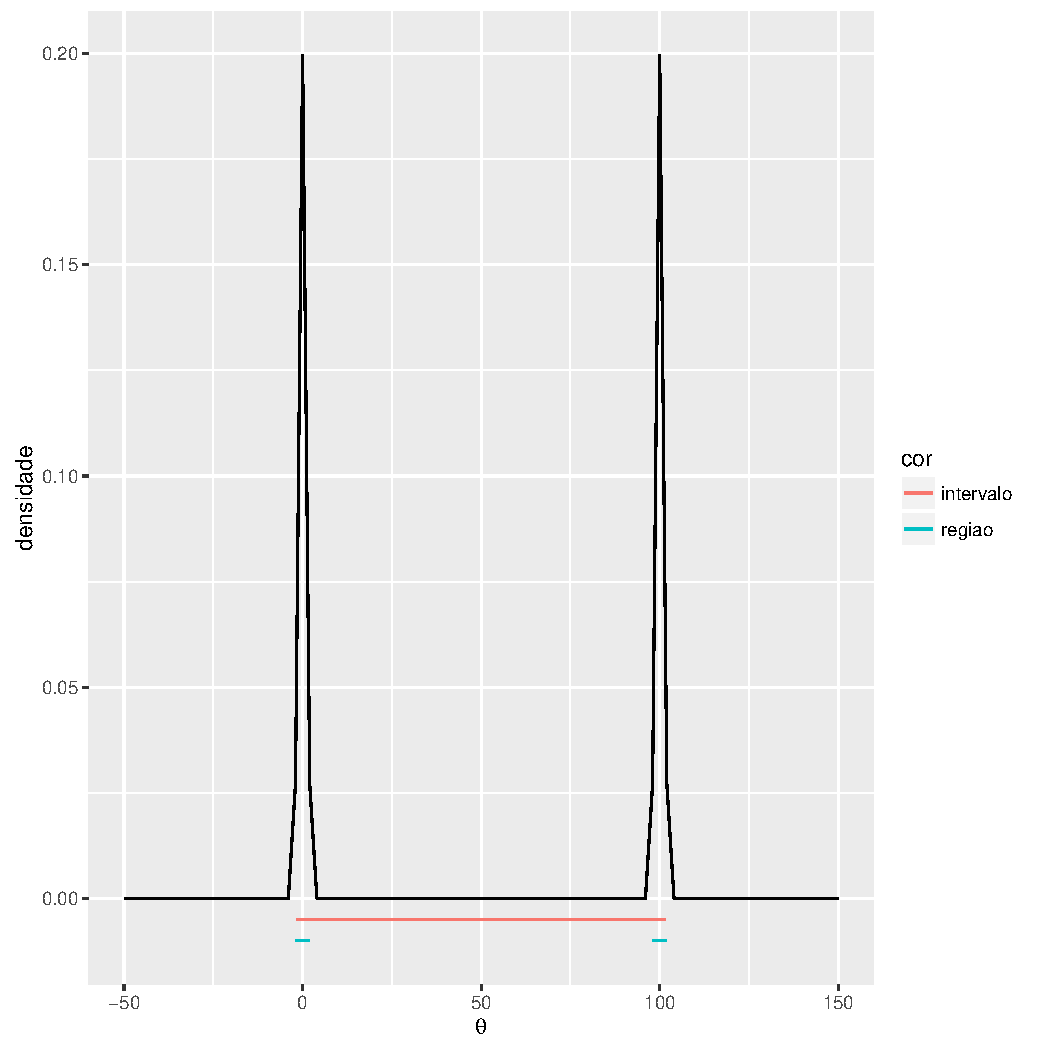
\includegraphics[scale=0.5]{chapter-decisions-normal-mixture.pdf}
\caption{Densidade da mistura de 
uma $N(0,1)$ e uma $N(100,1)$
acompanhada de um intervalo de credibilidade e
de uma região de credibilidade.}
\label{figure:normal-mixture-1}
\end{figure}

Como uma alternativa a um 
intervalo de credibilidade,
poderíamos combinar um 
intervalo de credibilidade para cada 
uma das normais na mistura.
Sabemos que uma $N(0,1)$ tem 
probabilidade de $95\%$ de estar em $[-1.96,1.96]$.
Similarmente, a $N(100,1)$ tem 
probabilidade de $95\%$ de estar em $[98.04,101.96]$.
Assim, a mistura de 
uma $N(0,1)$ e uma $N(100,1)$ tem 
alta probabilidade de estar em 
$[-1.96,1.96] \cup [98.04,101.96]$.
Neste exemplo, intervalos são 
demasiadamente restritivos e 
não descrevem adequadamente 
a \emph{posteriori} multimodal.

Assim, nesta subseção consideraremos 
um problema de decisão em que,
ao invés de escolher um intervalo para 
descrever a posteriori,
é necessário escolher uma região para fazê-lo.
De forma geral, uma região pode ser 
qualquer subconjunto do espaço paramétrico.
Assim, temos que
$\mathcal{A}_{*} = \{R \subset \Theta\}$.
Para estudar este problema de decisão,
consideraremos a seguinte função de utilidade
\begin{align*}
U(R(X),\theta)	
&= \I(\theta \in R(X)) 
-k\int_{x \in R(x)}{1 \cdot d\theta_0}
& k > 0
\end{align*}
O elemento $\I(\theta \in R(X))$ indica que 
é desejável que $\theta$ esteja 
na região de credibilidade, $R(X)$.
Por outro lado,  $\int_{x \in R(x)}{d\theta_0}$ indica que
é desejável que a região $R(x)$ seja pequena, 
ou seja, tenha um volume pequeno.
\begin{theorem}
\label{thm:hpd}
Se $U(R(X),\theta)	= \I(\theta \in R(X)) - k\int_{\theta_0 \in R(x)}{1 \cdot d\theta_0}$, então 
a melhor região de credibilidade é tal que 
$R(X) = \{\theta \in \Theta: f(\theta|X) \geq k\}$.
Dizemos que $R(X)$ é um HPD (highest posterior density) 
de $f(\theta|X)$.
Entre todas as regiões que têm uma dada probabilidade,
$R(X)$ também é a menor delas.
\end{theorem}


\subsubsection{Regiões de credibilidade com credibilidade especificada}
\label{sec:credibilidade}


Na prática, é comum criar uma região de credibilidade
de modo que a probabilidade (a posteriori) do parâmetro estar nessa região
seja um valor pré-especificado $1-\alpha$. Este valor de cobertura é chamado de 
\emph{credibilidade} dessa região:
\begin{definition}
Dizemos que uma região $R \subset \Theta$ tem credibilidade $1-\alpha$
se $\P(\theta \in R|\x)=1-\alpha$.
\end{definition}

Assim, é comum escolher o formato da região desejada usando 
alguma das funções de perda apresentadas nesta seção, e então buscar, dentre essas regiões,
aquela que tem a credibilidade desejada.

\begin{example}
Considere novamente o Exemplo \ref{exemplo:eleicao}.
Vamos construir intervalos de credibilidade
para $\theta$.
Para tanto, lembre-se que $\theta|X=20 \sim \mbox{Beta}(25,15)$.
O seguinte código ilustra como encontrar os intervalos de credibilidade
investigados nesta seção, com constantes na utilidade escolhidas de modo que a credibilidade dos intervalos seja $95\%$.
Neste caso, como a distribuição é próxima de ser simétrica, os três intervalos são muito próximos (\cref{fig:intervalos}).

\begin{knitrout}
\definecolor{shadecolor}{rgb}{0.969, 0.969, 0.969}\color{fgcolor}\begin{kframe}
\begin{alltt}
\hlstd{a} \hlkwb{<-} \hlnum{25} \hlcom{# hiperparâmetro a posteriori}
\hlstd{b} \hlkwb{<-} \hlnum{15} \hlcom{# hiperparâmetro a posteriori}

\hlstd{grid_theta} \hlkwb{<-} \hlkwd{seq}\hlstd{(}\hlnum{0}\hlstd{,}\hlnum{1}\hlstd{,}\hlkwc{length.out} \hlstd{=} \hlnum{1000}\hlstd{)}
\hlstd{aux} \hlkwb{=} \hlkwd{plot}\hlstd{(grid_theta,}
     \hlkwd{dbeta}\hlstd{(grid_theta,a,b),}
     \hlkwc{type}\hlstd{=}\hlstr{"l"}\hlstd{,}\hlkwc{lwd}\hlstd{=}\hlnum{3}\hlstd{,}\hlkwc{xlab} \hlstd{=} \hlkwd{expression}\hlstd{(theta),}\hlkwc{cex.lab}\hlstd{=}\hlnum{1.2}\hlstd{,}
     \hlkwc{ylab}\hlstd{=}\hlstr{"Densidade a posteriori"}\hlstd{)}

\hlcom{# função auxiliar para determinar a cobertura de um intervalo}
\hlstd{cobertura} \hlkwb{<-} \hlkwa{function}\hlstd{(}\hlkwc{limites}\hlstd{,}\hlkwc{a}\hlstd{,}\hlkwc{b}\hlstd{)}
\hlstd{\{}
  \hlkwd{return}\hlstd{(}\hlkwd{pbeta}\hlstd{(limites[}\hlnum{2}\hlstd{],a,b)}\hlopt{-}\hlkwd{pbeta}\hlstd{(limites[}\hlnum{1}\hlstd{],a,b))}
\hlstd{\}}

\hlstd{intervalo1} \hlkwb{<-} \hlkwa{function}\hlstd{(}\hlkwc{K}\hlstd{,}\hlkwc{a}\hlstd{,}\hlkwc{b}\hlstd{,}\hlkwc{grid_theta}\hlstd{)}
\hlstd{\{}
  \hlstd{soma} \hlkwb{<-} \hlkwd{sum}\hlstd{(}\hlkwd{dbeta}\hlstd{(grid_theta,a,b))}
  \hlstd{lim_inf} \hlkwb{<-} \hlkwd{min}\hlstd{(grid_theta[}\hlkwd{dbeta}\hlstd{(grid_theta,a,b)}\hlopt{>}\hlstd{K])}
  \hlstd{lim_sup} \hlkwb{<-} \hlkwd{max}\hlstd{(grid_theta[}\hlkwd{dbeta}\hlstd{(grid_theta,a,b)}\hlopt{>}\hlstd{K])}
  \hlkwd{return}\hlstd{(}\hlkwd{c}\hlstd{(lim_inf,lim_sup))}
\hlstd{\}}

\hlcom{# cobertura real menos 1-alpha}
\hlstd{funcao_para_minimizar} \hlkwb{<-} \hlkwa{function}\hlstd{(}\hlkwc{K}\hlstd{,}\hlkwc{alpha}\hlstd{,}\hlkwc{a}\hlstd{,}\hlkwc{b}\hlstd{,}\hlkwc{grid_theta}\hlstd{)}
\hlstd{\{}
  \hlstd{limites} \hlkwb{<-} \hlkwd{intervalo1}\hlstd{(K,a,b,grid_theta)}
  \hlkwd{return}\hlstd{(}\hlkwd{abs}\hlstd{(}\hlkwd{cobertura}\hlstd{(limites,a,b)}\hlopt{-}\hlstd{(}\hlnum{1}\hlopt{-}\hlstd{alpha)))}
\hlstd{\}}

\hlstd{melhor_k} \hlkwb{<-} \hlkwd{optim}\hlstd{(}\hlkwc{par} \hlstd{=} \hlkwd{max}\hlstd{(}\hlkwd{dbeta}\hlstd{(grid_theta,a,b))}\hlopt{/}\hlnum{2}\hlstd{,funcao_para_minimizar,}\hlkwc{alpha}\hlstd{=}\hlnum{0.05}\hlstd{,}
      \hlkwc{a}\hlstd{=a,}\hlkwc{b}\hlstd{=b,}
      \hlkwc{grid_theta}\hlstd{=grid_theta,}
      \hlkwc{lower}\hlstd{=}\hlnum{0}\hlstd{,}
      \hlkwc{upper}\hlstd{=}\hlkwd{max}\hlstd{(}\hlkwd{dbeta}\hlstd{(grid_theta,a,b)),}\hlkwc{method} \hlstd{=} \hlstr{"L-BFGS-B"}\hlstd{)}
\hlstd{K} \hlkwb{<-} \hlstd{melhor_k}\hlopt{$}\hlstd{par}
\hlstd{limites1} \hlkwb{<-} \hlkwd{intervalo1}\hlstd{(K,a,b,grid_theta)}

\hlstd{intervalo2} \hlkwb{<-} \hlkwa{function}\hlstd{(}\hlkwc{alpha}\hlstd{,}\hlkwc{a}\hlstd{,}\hlkwc{b}\hlstd{)}
\hlstd{\{}
  \hlcom{# esperança e variância a posteriori}
  \hlstd{lim_inf} \hlkwb{<-} \hlkwd{qbeta}\hlstd{(alpha}\hlopt{/}\hlnum{2}\hlstd{,a,b)}
  \hlstd{lim_sup} \hlkwb{<-} \hlkwd{qbeta}\hlstd{(}\hlnum{1}\hlopt{-}\hlstd{alpha}\hlopt{/}\hlnum{2}\hlstd{,a,b)}
  \hlkwd{return}\hlstd{(}\hlkwd{c}\hlstd{(lim_inf,lim_sup))}
\hlstd{\}}
\hlstd{limites2} \hlkwb{<-} \hlkwd{intervalo2}\hlstd{(}\hlnum{0.05}\hlstd{,a,b)}

\hlstd{intervalo3} \hlkwb{<-} \hlkwa{function}\hlstd{(}\hlkwc{K}\hlstd{,}\hlkwc{a}\hlstd{,}\hlkwc{b}\hlstd{)}
\hlstd{\{}
  \hlcom{# esperança e variância a posteriori}
  \hlstd{esp_theta} \hlkwb{<-} \hlstd{a}\hlopt{/}\hlstd{(a}\hlopt{+}\hlstd{b)}
  \hlstd{var_theta} \hlkwb{<-} \hlstd{a}\hlopt{*}\hlstd{b}\hlopt{/}\hlstd{((a}\hlopt{+}\hlstd{b}\hlopt{+}\hlnum{1}\hlstd{)}\hlopt{*}\hlstd{(a}\hlopt{+}\hlstd{b)}\hlopt{^}\hlnum{2}\hlstd{)}

  \hlstd{lim_inf} \hlkwb{<-} \hlstd{esp_theta}\hlopt{-}\hlstd{K}\hlopt{*}\hlkwd{sqrt}\hlstd{(var_theta)}
  \hlstd{lim_sup} \hlkwb{<-} \hlstd{esp_theta}\hlopt{+}\hlstd{K}\hlopt{*}\hlkwd{sqrt}\hlstd{(var_theta)}
  \hlkwd{return}\hlstd{(}\hlkwd{c}\hlstd{(lim_inf,lim_sup))}
\hlstd{\}}

\hlcom{# cobertura real menos 1-alpha}
\hlstd{funcao_para_minimizar} \hlkwb{<-} \hlkwa{function}\hlstd{(}\hlkwc{K}\hlstd{,}\hlkwc{alpha}\hlstd{,}\hlkwc{a}\hlstd{,}\hlkwc{b}\hlstd{)}
\hlstd{\{}
  \hlstd{limites} \hlkwb{<-} \hlkwd{intervalo3}\hlstd{(K,a,b)}
  \hlkwd{return}\hlstd{(}\hlkwd{abs}\hlstd{(}\hlkwd{cobertura}\hlstd{(limites,a,b)}\hlopt{-}\hlstd{(}\hlnum{1}\hlopt{-}\hlstd{alpha)))}
\hlstd{\}}

\hlstd{melhor_k} \hlkwb{<-} \hlkwd{optim}\hlstd{(}\hlkwc{par} \hlstd{=} \hlkwd{max}\hlstd{(}\hlkwd{dbeta}\hlstd{(grid_theta,a,b))}\hlopt{/}\hlnum{2}\hlstd{,funcao_para_minimizar,}\hlkwc{alpha}\hlstd{=}\hlnum{0.05}\hlstd{,}
      \hlkwc{a}\hlstd{=a,}\hlkwc{b}\hlstd{=b,}
      \hlkwc{lower}\hlstd{=}\hlnum{0}\hlstd{,}
      \hlkwc{upper}\hlstd{=}\hlkwd{max}\hlstd{(}\hlkwd{dbeta}\hlstd{(grid_theta,a,b)),}\hlkwc{method} \hlstd{=} \hlstr{"L-BFGS-B"}\hlstd{)}
\hlstd{K} \hlkwb{<-} \hlstd{melhor_k}\hlopt{$}\hlstd{par}
\hlstd{limites3} \hlkwb{<-} \hlkwd{intervalo3}\hlstd{(K,a,b)}

\hlstd{aux}
\end{alltt}
\begin{verbatim}
## NULL
\end{verbatim}
\begin{alltt}
\hlkwd{lines}\hlstd{(limites1,}\hlkwd{c}\hlstd{(}\hlnum{0.05}\hlstd{,}\hlnum{0.05}\hlstd{),}\hlkwc{lwd}\hlstd{=}\hlnum{3}\hlstd{)}
\hlkwd{lines}\hlstd{(limites2,}\hlkwd{c}\hlstd{(}\hlnum{0.15}\hlstd{,}\hlnum{0.15}\hlstd{),}\hlkwc{lwd}\hlstd{=}\hlnum{3}\hlstd{,}\hlkwc{col}\hlstd{=}\hlnum{2}\hlstd{)}
\hlkwd{lines}\hlstd{(limites3,}\hlkwd{c}\hlstd{(}\hlnum{0.25}\hlstd{,}\hlnum{0.25}\hlstd{),}\hlkwc{lwd}\hlstd{=}\hlnum{3}\hlstd{,}\hlkwc{col}\hlstd{=}\hlnum{4}\hlstd{)}
\hlkwd{legend}\hlstd{(}\hlnum{0}\hlstd{,}\hlnum{5}\hlstd{,}\hlkwc{col}\hlstd{=}\hlkwd{c}\hlstd{(}\hlnum{1}\hlstd{,}\hlnum{2}\hlstd{,}\hlnum{4}\hlstd{),}\hlkwc{legend} \hlstd{=} \hlkwd{c}\hlstd{(}\hlstr{"Tipo 1"}\hlstd{,}\hlstr{"Tipo 2"}\hlstd{,}\hlstr{"Tipo 3"}\hlstd{),}\hlkwc{lwd}\hlstd{=}\hlnum{3}\hlstd{)}
\end{alltt}
\end{kframe}\begin{figure}[t]

{\centering 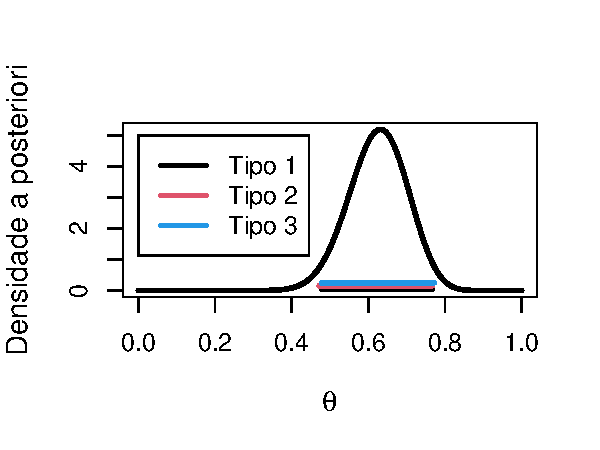
\includegraphics[width=\maxwidth]{./figures/intervalos-1} 

}

\caption[Intervalos de credibilidade]{Intervalos de credibilidade}\label{fig:intervalos}
\end{figure}

\end{knitrout}


\end{example}

\subsubsection*{Exercícios}

\begin{exercise}
\label{ex:normal-credible}
Dado $\mu$, $X_{1},\ldots,X_{n}$ são i.i.d. e 
$X_{1} \sim N(\mu,1)$.
\emph{A priori}, $\mu \sim N(0,1)$.
\begin{enumerate}[label=(\alph*)]
\item Ache um estimador para $\mu$ usando 
cada utilidade que vimos em aula.
\item Ache um intervalo para $\mu$ com 
credibilidade $95\%$ para 
cada utilidade que vimos em aula.
\item Ache o HPD para $\mu$.
\end{enumerate}
\end{exercise}

\solution{\textbf{Solução}:
Decorre do \cref{ex:conjugate-normal-normal} que
$\theta|X \sim N(\frac{n\bar{X}}{n+1},n+1)$.
\begin{enumerate}[label=(\alph*)]
\item Sabemos que, para a distância quadrática
(\cref{thm:estimation_l2}), 
o estimador ótimo é $E[\theta|X]$ e,
para a distância em valor absoluto
(\cref{thm:estimation_l1}), ele é $Med[\theta|X]$.
Como a distribuição normal é 
simétrica em torno da média, temos que 
$Med[\theta|X] = E[\theta|X] = \frac{n\bar{X}}{n+1}$.

\item \begin{itemize}
\item Como a distribuição normal é unimodal,
o intervalo de credibilidade pelo
\cref{thm:credible_interval_1} é da forma 
\begin{align*}
[a,b] = \{\theta \in \Theta: f(\theta|X) \geq k\}
\end{align*}
Também, como a distribuição normal é 
simétrica em torno de $\E[\theta|X]$ e unimodal,
existe $c$ tal que
\begin{align*}
\{\theta \in \Theta: f(\theta|X) \geq k\} 
&= [\E[\theta|X]-c,\E[\theta|X]+c]
\end{align*}
Assim, desejamos achar $c$ tal que
\begin{align*}
\P(\theta \in [\E[\theta|X]-c,\E[\theta|X]+c]|X)
&= 95\%	\\
\P\left(\frac{\theta
-\E[\theta|X]}{\sqrt{\V[\theta|X]}} 
\in \left[-\frac{c}{\sqrt{\V[\theta|X]}},
\frac{c}{\sqrt{\V[\theta|X]}}\right]|X\right)	
&= 95\%
\end{align*}
Como $\frac{\theta-\E[\theta|X]}{\V[\theta|X]}|X \sim N(0,1)$, $\frac{c}{\sqrt{\V[\theta|X]}}=1.96$.
Como $\theta|X$ tem variância $(n+1)^{-1}$,
obtemos o intervalo
\begin{align*}
\left[\frac{n\bar{X}}{n+1}-1.96(n+1)^{-0.5},
\frac{n\bar{X}}{n+1}+1.96(n+1)^{-0.5}\right]
\end{align*}

\item Usando o \cref{thm:credible_interval_2}, 
obtemos um intervalo $[a,b]$ tal que 
$\P(\theta < a|X) = 2.5\%$ e 
$\P(\theta > b|X) = 2.5\%$.
\begin{align*}
\P(\theta < a|X) &= 2.5\% \\
\P\left(\frac{\theta-\E[\theta|X]}
{\sqrt{\V[\theta|X}} 
< \frac{a-\E[\theta|X]}{\sqrt{\V[\theta|X}}|X\right)
&= 2.5\%
\end{align*}
Como $\frac{\theta-\E[\theta|X]}{\sqrt{\V[\theta|X]}}|X \sim N(0,1)$, 
$\frac{a-\E[\theta|X]}{\sqrt{\V[\theta|X}}=-1.96$.
Como a $\theta|X$ é simétrica em torno de
$\E[\theta|X]$, 
$\frac{b-\E[\theta|X]}{\sqrt{\V[\theta|X}}=1.96$.
Assim, obtemos o intervalo
\begin{align*}
\left[\frac{n\bar{X}}{n+1}-1.96(n+1)^{-0.5},
\frac{n\bar{X}}{n+1}+1.96(n+1)^{-0.5}\right]
\end{align*}

\item Usando o \cref{thm:credible_interval_3}, 
obtemos um intervalo $[a,b]$ da forma
\begin{align*}
[a,b]
&= \left[\E[\theta|X]-c\sqrt{\V[\theta|X]},
\E[\theta|X]+c\sqrt{\V[\theta|X]}\right]
\end{align*}
Sabemos pelos itens anteriores que este 
intervalo tem credibilidade $95\%$ somente se 
$c=1.96$. Assim, obtemos o intervalo
\begin{align*}
\left[\frac{n\bar{X}}{n+1}-1.96(n+1)^{-0.5},
\frac{n\bar{X}}{n+1}+1.96(n+1)^{-0.5}\right]
\end{align*}
\end{itemize}

No caso da distribuição normal,
que é unimodal e simétrica em torno de sua média,
todos os intervalos de credibilidade são equivalentes.

\item Como a distribuição a posteriori é unimodal,
o HPD é equivalente ao intervalo de credibilidade 
obtido no \cref{thm:credible_interval_1}.
Assim, o HPD é
\begin{align*}
\left[\frac{n\bar{X}}{n+1}-1.96(n+1)^{-0.5},
\frac{n\bar{X}}{n+1}+1.96(n+1)^{-0.5}\right]
\end{align*}
\end{enumerate}
}{}

\begin{exercise}
Considere que $\theta|X \sim \text{Beta(0.05,0.05)}$.
\begin{enumerate}[label=(\alph*)]
\item $f(\theta|X)$ é uma função côncava?
\item Use um \emph{software} estatístico para 
achar um intervalo de credibilidade para $\theta|X$.
\item Use um \emph{software} estatístico para 
achar um HPD para $\theta|X$.
\end{enumerate}
\end{exercise}

\solution{\textbf{Solução}:
\begin{enumerate}[label=(\alph*)]
\item Note que $f(\theta|X) = \beta^{-1}(0.05,0.05)\theta^{-0.95}(1-\theta)^{-0.95}$.
A densidade a posteriori é indicada na  
\cref{figure:bimodal-beta}.
Note que $f(0|X) = f(1|X) = \infty$.
Se $f$ é côncava, $a < b$ e $f(a) < f(b)$,
então $f$ é decrescente a partir de $a$.
Como $0 < 0.5 < 1$, 
$f(0|X) > f(0.5|X)$ e 
$f(0.5|X) < f(1|X)$,
$f(\theta|X)$ não é côncava.	
\begin{figure}
\centering
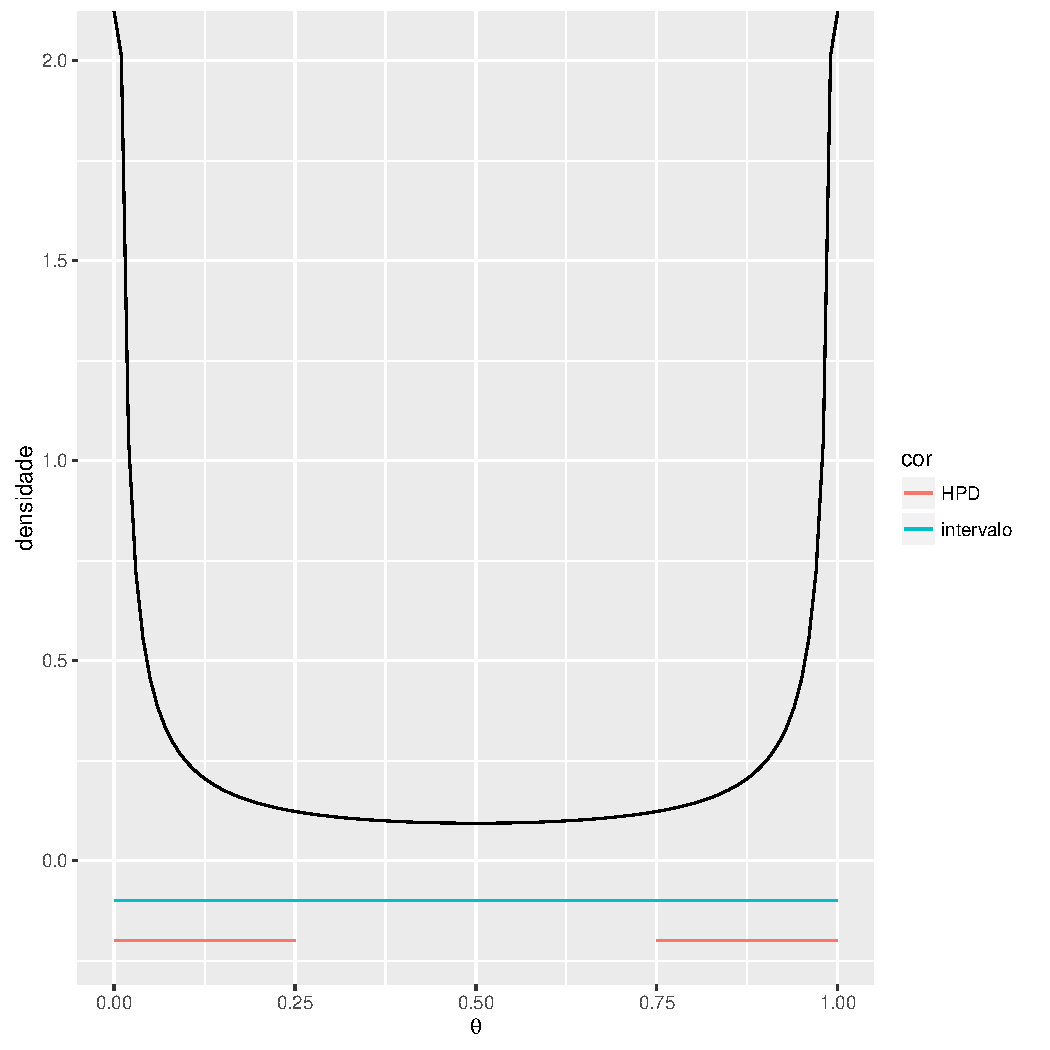
\includegraphics[scale=0.5]{chapter-decisions-bimodal-beta.pdf}
\caption{Densidade da Beta$(0.05,0.05)$
acompanhada de um intervalo de credibilidade 
e o HPD.}
\label{figure:bimodal-beta}
\end{figure}

\item Usando o \cref{thm:credible_interval_2},
um possível intervalo de credibilidade, $[a,b]$,
é tal que $\P(\theta < a|X) = 2.5\%$ e 
$\P(\theta > b|X) = 2.5\%$.
Podemos usar a função $qbeta$ no $R$ para
obter os percentis da Beta$(0.05,0.05)$.
O $R$ indica que eles são $8.8e-27$ e $1$.
Portanto, o intervalo de credibilidade é
praticamente o intervalo $[0,1]$ inteiro.

\item Note pela \cref{figure:bimodal-beta} que 
as regiões de maior densidade são
os valores extremos à esquerda e à direita.
Portanto, o HPD é composto por estes extremos.
Como a distribuição a posteriori é simétrica em 
torno de $0.5$,
O HPD pode ser obtido determinando 
$\P(\theta < a|X) = 47.5\%$ e
$\P(\theta > b|X) = 52.5\%$.
O HPD será $[0,a] \cup [b,1]$.
Usando o $R$ encontramos que 
$a \approx 0.25$ e $b \approx 0.75$.
\end{enumerate}
}{}

\begin{exercise}[Sugestão de Aline Tonon]
Considere o problema de determinar um intervalo de credibilidade, $(a,b)$, com a função de utilidade, $U((a,b),\theta)=\frac{\I(\theta \in (a,b))}{b-a}$. Prove que, se $(a^*,b^*)$ é um intervalo de credibilidade ótimo, então $f_{\theta|X}(a^*|X)=f_{\theta|X}(b^*|X)$.
\end{exercise}

\solution{\textbf{Solução}: Defina
\begin{align*}
g(a,b) := \E\left[U((a,b),\theta)|X\right]
&= \E\left[\frac{\I(\theta \in (a,b))}{b-a}\bigg|X\right]
= \frac{F_{\theta|X}(b|X)-F_{\theta|X}(a|X)}{b-a}
\end{align*}
Para que um ponto $(a,b)$ maximize $g(a,b)$,
ele deve ser tal que $\nabla g(a,b)=\textbf{0}$.
Note que
\begin{align*}
\nabla g(a,b) &= \left(\frac{\partial \frac{F_{\theta|X}(b|X)-F_{\theta|X}(a|X)}{b-a}}{\partial a}, \frac{\partial \frac{F_{\theta|X}(b|X)-F_{\theta|X}(a|X)}{b-a}}{\partial b}\right) \\
&= \left(-\frac{f_{\theta|X}(a|X)(b-a)+(F_{\theta|X}(b|X)-F_{\theta|X}(a|X))}{(b-a)^2}, \frac{f_{\theta|X}(b|X)(b-a)-(F_{\theta|X}(b|X)-F_{\theta|X}(a|X))}{(b-a)^2} \right)
\end{align*}
Portanto, para que $\nabla g(a,b) = \textbf{0}$,
obtemos
\begin{align*}
\begin{cases}
f_{\theta|X}(a|X) = \frac{F_{\theta|X}(b|X)-F_{\theta|X}(a|X)}{b-a} \\
f_{\theta|X}(b|X) = \frac{F_{\theta|X}(b|X)-F_{\theta|X}(a|X)}{b-a}
\end{cases}
\end{align*}
Conclua que, se $(a^*,b^*)$ maximiza 
a utilidade esperada, então
$f_{\theta|X}(a^*|X)=f_{\theta|X}(b^*|X)$.
}{}

\begin{exercise}
Considere o problema de determinar um intervalo de credibilidade, $(a,b)$, com a função de utilidade, $U((a,b),\theta)=\frac{k-(a-\theta)_{+}-(b-\theta)_{+}}{b-a}$. Prove que, se $(a^*,b^*)$ é um intervalo de credibilidade ótimo, então
$F_{\theta|X}(a^*|X)=1-F_{\theta|X}(b^*|X)$.
\end{exercise}

\solution{\textbf{Solução}: Defina
\begin{align*}
g(a,b) := \E\left[U((a,b),\theta)|X\right]
&= \E\left[\frac{k-(a-\theta)_{+}-(b-\theta)_{+}}{b-a}\bigg|X\right] \\
&= \frac{k-\int_{-\infty}^{a}{(a-\theta)f_{\theta|X}(t|X)dt} -\int_{b}^{\infty}{(\theta-b)f_{\theta|X}(t|X)dt}}{b-a}
\end{align*}
Defina $h(a,b) := k-\int_{-\infty}^{a}{(a-\theta)f_{\theta|X}(t|X)dt} -\int_{b}^{\infty}{(\theta-b)f_{\theta|X}(t|X)dt}$.
Para que um ponto $(a,b)$ maximize $g(a,b)$,
ele deve ser tal que $\nabla g(a,b)=\textbf{0}$.
Note que
\begin{align*}
\nabla g(a,b) &= \left(\frac{\partial g(a,b)}{\partial a}, \frac{\partial g(a,b)}{\partial b}\right) \\
&= \left(\frac{-(b-a)\int_{-\infty}^{a}{f_{\theta|X}(t|X)dt} + h(a,b)}{(b-a)^2}, \frac{(b-a)\int_{b}^{\infty}{f_{\theta|X}(t|X)dt}-h(a,b)}{(b-a)^2} \right)
\end{align*}
Portanto, para que $\nabla g(a,b) = \textbf{0}$,
é necessário que
\begin{align*}
\begin{cases}
\int_{\infty}^{a}{f_{\theta|X}(t|X)dt} = 
\frac{h(a,b)}{b-a}\\
\int_{b}^{\infty}{f_{\theta|X}(t|X)dt} = 
\frac{h(a,b)}{b-a}
\end{cases}
\end{align*}
Conclua que, se $(a^*,b^*)$ maximiza a
utilidade esperada, então
$\int_{\infty}^{a^*}{f_{\theta|X}(t|X)dt}=\int_{b^*}^{\infty}{f_{\theta|X}(t|X)dt}$,
isto é, 
$F_{\theta|X}(a^*|X)=1-F_{\theta|X}(b^*|X)$.
}{}


\subsection{Testes de hipótese}

Um problema de teste de hipótese consiste
em escolher uma entre duas proposições 
disjuntas e mutuamente exclusivas.
Neste contexto, estas proposições recebem
nomes especiais: uma delas é a hipótese nula e
a outra é a hipótese alternativa.
Denotaremos a hipótese nula por $H_{0}$ e
a hipótese alternativa por $H_{1}$.

\begin{example}
 \label{example:hyp-binomial}
 Uma máquina pode estar regulada ou desregulada.
 Caso a máquina esteja regulada, 
 ela produz componentes com uma taxa de falha de 5\%.
 Caso a máquina esteja desregulada,
 ela produz componentes com uma taxa de falha de 20\%.
 Uma amostra de $100$ produtos é selecionada e 
 $9$ deles são defeituosos.
 
 Sejam $X_{1},\ldots,X_{n}$ as indicadoras de que
 cada peça amostrada é defeituosa e 
 $\theta$ é a taxa de falha atual da máquina, 
 $\theta \in \{5\%, 20\%\}$.
 Consideramos que, dado 
 $\theta$, $X_{1},\ldots,X_{n}$ são i.i.d. e
 $\sum_{i=1}^{100}{X_{i}}|\theta \sim \text{Binomial}(100,\theta)$.

 Podemos estar interessados em testar a hipótese de
 que a máquina está regulada contra 
 a hipótese de que ela está desregulada.
 Neste caso, $H_{0} = \{\theta = 5\%\}$ e 
 $H_{1} = \{\theta = 20\%\}$.
\end{example}

\begin{example}
 \label{example:hyp-binomial-predictive}
 Considere a mesma descrição do \cref{example:hyp-binomial}.
 Seja $X_{n+1}$ a indicadora de que 
 uma nova peça produzida pela máquina é defeituosa.
 Podemos testar a hipótese de que
 esta peça é defeituosa.
 Neste caso, $H_{0} = \{X_{n+1}=0\}$ e 
 $H_{1} = \{X_{n+1}=1\}$.
\end{example}

\begin{example}
 \label{example:hyp-logistica}
 Considere o \cref{ex:normal-mixture}.
 Seja $\theta$ a indicadora de que 
 a pessoa selecionada é uma mulher.
 Podemos testar $H_{0}=\{\theta=0\}$ contra 
 $H_{1}=\{\theta=1\}$. 
\end{example}

\begin{example}
 \label{example:hyp-linear-regression}
 Em um experimento, 
 larga-se uma pedra de uma determinada altura e 
 mede-se a sua posição relativa ao ponto de largada
 a cada $1$ segundo.
 Se $Y_{i}$ denota a posição relativa da pedra 
 no segundo $i$,
 assumimos que $Y_{i} = -g\frac{i^{2}}{2} + \epsilon_{i}$,
 onde $\epsilon_{i}$ são i.i.d. e 
 $\epsilon_{i} \sim N(0,1)$,
 com $\tau^{2}$ conhecido.

 Podemos testar a hipótese $H_{0} = \{g = 10\}$ contra 
 a hipótese $H_{1} = \{g \neq 10\}$.
 Semelhantemente, podemos testar a hipótese 
 $H_{0} = \{g \geq 10\}$ contra $H_{1} = \{g < 10\}$.
\end{example}

\begin{table}
 \centering
 \begin{tabular}{|c|c|c|}
  \hline
  & $\theta \in H_{0}$	& $\theta \in H_{1}$ \\
  \hline 
  d=0 & 0 & -1 \\
  d=1 & -c & 0 \\
  \hline
 \end{tabular}
 \caption{Descrição dos valores da utilidade 
 $0-1-c$, $U(d,\theta)$.}
 \label{table:u-0-1-c}
\end{table}

Você deve escolher entre $H_{0}$ e $H_{1}$.
Assim, ao tentar expressar um teste de hipótese como
um problema de decisão,
é comum definir $\mathcal{A}_{*} = \{0,1\}$,
onde $0$ significa não rejeitar $H_{0}$ e 
$1$ significa rejeitar $H_{0}$.

\subsubsection{Hipóteses plenas}

É comum o uso da função de utilidade $0-1-c$,
descrita na \cref{table:u-0-1-c}.
Dizemos que rejeitar $H_{0}$ quando 
$H_{0}$ é verdadeiro é um erro do tipo I.
Também, não rejeitar $H_{0}$ quando 
$H_{1}$ é verdadeiro é um erro do tipo II.
Na \cref{table:u-0-1-c},
o valor de $c$ indica o quanto o erro de tipo I
é mais grave que o erro de tipo II.
Se $c > 1$, o erro de tipo I é mais grave que
o erro de tipo II.
Se $c < 1$, o erro de tipo I é menos grave que
o erro de tipo II.
Se $c = 1$, então ambos os erros são igualmente graves.

Segundo estas condições,
podemos calcular uma regra ótima de decisões.

\begin{theorem}
 \label{thm:0-1-c}
 Em um problema de teste de hipótese com a utilidade
 dada pela \cref{table:u-0-1-c},
 as decisões ótimas, $\delta^{*}$, são tais que
 \begin{align*}
  \delta^{*}(x)	&=
  \begin{cases}
   0, & \text{ se } 
   \P(\theta \in H_{0}|x) > (1+c)^{-1} \\
   1, & \text{ se } 
   \P(\theta \in H_{0}|x) < (1+c)^{-1}
  \end{cases}
 \end{align*}
\end{theorem}

\begin{proof}
 Decorre do \cref{theorem:extensive-form} que
 a decisão ótima, $\delta^{*}$, é aquela que, 
 para cada valor de $X$, 
 maximiza $\E[U(d,\theta)|X]$.
 Para cada valor de $X$, somente existem 
 $2$ possíveis decisões (0 ou 1).
 Assim, a $\delta^{*}$ é tal que
 \begin{align}
  \label{eqn:0-1-c-1}
  \delta^{*}(x)	&=
  \begin{cases}
   0, & \text{ se } 
   \E[U(0,\theta)|X] > \E[U(1,\theta)|X] \\
   1, & \text{ se } 
   \E[U(0,\theta)|X] < \E[U(1,\theta)|X]
  \end{cases}
 \end{align}
 Note que
 \begin{align*}
  \E[U(0,\theta)|X]	
  &= \E[U(0,\theta)\I(\theta \in H_{0})|X]
  +\E[U(0,\theta)\I(\theta \in H_{1})|X] \\
  &= \E[0 \cdot \I(\theta \in H_{0})|X] 
  +\E[-1 \cdot \I(\theta \in H_{1})|X] \\
  &= -1 \cdot \E[\I(\theta \in H_{1})|X] 
  = -\P(\theta \in H_{1}|X)
 \end{align*}
 \begin{align*}
  \E[U(1,\theta)|X]	
  &= \E[U(1,\theta)\I(\theta \in H_{0})|X] 
  +\E[U(1,\theta)\I(\theta \in H_{1})|X] \\
  &=\E[-c \cdot \I(\theta \in H_{0})|X] 
  +\E[0 \cdot \I(\theta \in H_{1})|X] \\
  &= -c \cdot \E[\I(\theta \in H_{0})|X] 
  =-c\P(\theta \in H_{0}|X)
 \end{align*}
 Utilizando as expressões derivadas acima 
 na \cref{eqn:0-1-c-1},
 obtemos que $\delta^{*}(x) = 0$ quando
 \begin{align*}
  -\P(\theta \in H_{1}|X) 
  &> -c\P(\theta \in H_{0}|X) \\
  -(1-\P(\theta \in H_{0}|X))
  &> -c\P(\theta \in H_{0}|X) \\
  -1 &> -(1+c)\P(\theta \in H_{0}|X) \\
  \P(\theta \in H_{0}|X) &> (1+c)^{-1}
 \end{align*}
 Semelhantemente, a decisão ótima é $1$ 
 quando $\P(\theta \in H_{0}|X)	< (1+c)^{-1}$.
\end{proof}

Em palavras, o \cref{thm:0-1-c} indica que 
a decisão ótima é não rejeitar $H_{0}$ quando 
sua probabilidade a posteriori é 
suficientemente grande.
Em especial, se $c=1$, temos que 
o erro tipo I é tão grave quanto o erro tipo II.
Neste caso, a regra de decisão ótima segundo 
o \cref{thm:0-1-c} é 
não rejeitar $H_{0}$ quando 
sua probabilidade a posteriori é 
maior do que $0.5$.

\begin{example}
 \label{example:hyp-binomial-2}
 Considere o \cref{example:hyp-binomial}. 
 Também considere que, a priori,
 $\P(H_{0})=\P(H_{1})=0.5$,
 e o erro de tipo I é considerado $2$ vezes 
 menos grave que o erro tipo II. Assim $c=0.5$.
 Neste caso,
 \begin{align*}
  \P\left(H_{0}|\sum_{i=1}^{100}{X_i}=9\right)
  &= \frac{\P(H_{0})P(\sum_{i=1}^{100}{X_i}=9|H_{0})}
  {\P(H_{0})\P(\sum_{i=1}^{100}{X_i}=9|H_{0})
  +\P(H_{1})\P(\sum_{i=1}^{100}{X_i}=9|H_{1})} \\
  &= \frac{0.5 {100 \choose 9}(0.05)^{9}(0.95)^{91}}{0.5 {100 \choose 9}(0.05)^{9}(0.95)^{91} + 0.5 {100 \choose 9}(0.2)^{9}(0.8)^{91}} \\
  &\approx 0.96
 \end{align*}
 Como $\P\left(H_{0}|\sum_{i=1}^{100}{X_i}=9\right) \approx 0.96 > 0.66 \approx (1+c)^{-1}$,
 a decisão ótima é não rejeitar $H_{0}$.
\end{example}

\begin{example}
 Considere o \cref{example:hyp-binomial-predictive}. 
 Também considere que, a priori, 
 $\P(H_{0})=\P(H_{1})=0.5$,
 e o erro de tipo I é considerado $9$ vezes 
 mais grave que o erro tipo II. Assim $c=9$.
 Temos
 \begin{align*}
  \P\left(X_{n+1}=0|\sum_{i=1}^{n}{X_{i}}=9\right)
  =& \P\left(X_{n+1}=0,\theta=0.05|\sum_{i=1}^{n}{X_{i}}=9\right)
  +\P\left(X_{n+1}=0,\theta=0.2|\sum_{i=1}^{n}{X_{i}}=9\right) \\
  =& \P(X_{n+1}=0|\theta=0.05)
  \P(\theta=0.05|\sum_{i=1}^{n}{X_{i}}=9)+\\
  & \P(X_{n+1}=0|\theta=0.2)
  \P(\theta=0.2|\sum_{i=1}^{n}{X_{i}}=9) \\
  \approx& 0.05 \cdot 0.96 + 0.2 \cdot 0.04 = 0.056
 \end{align*}
 Como $\P\left(X_{n+1}=0|\sum_{i=1}^{n}{X_{i}}=9\right) = 0.056 < 10^{-1} = (1+c)^{-1}$,
 rejeitamos $H_{0}$.
\end{example}

\begin{example}
 Considere o \cref{example:hyp-logistica}. 
 Também considere que, a priori, 
 $\P(H_{0})=\P(H_{1})=0.5$,
 e o erro de tipo I é considerado tão 
 grave quanto o erro tipo II. Assim $c=1$.
 Pelo \cref{ex:normal-mixture}, sabemos que
 \begin{align*}
  \P(H_{1}|x)
  &=\frac{1}{1 + \exp\left(\frac{10x-1675}{18}\right)}
 \end{align*}
 Pelo \cref{thm:0-1-c}, rejeitamos $H_{0}$ quando
 $\P(H_{1}|x) > (1+c)^{-1} = 0.5$.
 Assim, rejeitamos $H_{0}$ se
 \begin{align*}
  \frac{1}{1+\exp\left(\frac{10x-1675}{18}\right)} 
  &> 0.5 \\
  1
  &> 0.5 + 0.5\exp\left(\frac{10x-1675}{18}\right) \\
  \exp\left(\frac{10x-1675}{18}\right) &< 1 \\
  x &< 167.5
 \end{align*}
 Dizemos que esse é um critério de decisão linear,
 dado que a regra de decisão pode ser 
 explicada observando se uma reta em função dos dados é
 maior ou menor que um determinado valor.
 
 Também note que, neste problema,
 a altura dos homens e mulheres seguem 
 distribuições normais com média 170cm e 165cm e 
 variâncias iguais.
 Assim, não é surpreendente que o critério de decisão
 é rejeitar que a pessoa é um homem se a sua altura
 for menor que $167.5$ a média simples entre 170 e 165.
\end{example}

\begin{comment}
 \begin{example}
 Considere o \cref{example:hyp-linear-regression} em que
 queremos testar $H_{0} = \{g \geq 10\}$ contra $H_{1} = \{g < 10\}$.
 Também considere que os erros tipo I e II são igualmente graves e
 que, \emph{a priori}, $g \sim N(0,1)$.
 
 Desejamos achar a distribuição \emph{a posteriori} de 
 $g|Y_{1},\ldots,Y_{n}$. Defina $x_{i}= -\frac{i^{2}}{2}$.
 Assim, temos um problema equivalente ao \cref{ex:simple-linear-regression}
 e obtemos
 $$g|(x_{1},y_{1}),\ldots,(x_{n},y_{n}) \sim N\left(\frac{\sum_{i=1}^{n}{x_{i}y_{i}}}{\left(1+\sum_{i=1}^{n}{x_{i}^{2}}\right)}, \left(1+\sum_{i=1}^{n}{x_{i}^{2}}\right)^{-1}\right)$$
 \end{example}
\end{comment}

\begin{corollary}
 \label{cor:0-1-c}
 Em um problema de teste de hipótese com 
 a utilidade dada pela \cref{table:u-0-1-c},
 as decisões ótimas, $\delta^{*}$, são tais que
 \begin{align*}
  \delta^{*}(x)	&=
  \begin{cases}
   0, & \text{ se } 
   \frac{\P(x|\theta \in H_{0})}{\P(x|\theta \in H_{1})}	
   > \frac{\P(\theta \in H_{1})}{c\P(\theta \in H_{0})} \\
   1, & \text{ se } 
   \frac{\P(x|\theta \in H_{0})}{\P(x|\theta \in H_{1})}
   < \frac{\P(\theta \in H_{1})}{c\P(\theta \in H_{0})}
  \end{cases}
 \end{align*}
\end{corollary}

\begin{proof}
 Podemos desenvolver a expressão 
 $\P(\theta \in H_{0}|x) > (1+c)^{-1}$ 
 da seguinte forma.
 \begin{align*}
  \P(\theta \in H_{0}|x) &> (1+c)^{-1}	\\
  \frac{\P(\theta \in H_{0})\P(x|\theta \in H_{0})}
  {\P(\theta \in H_{0})\P(x|\theta \in H_{0}) 
  +\P(\theta \in H_{1})\P(x|\theta \in H_{1})}
  &> (1+c)^{-1}	\\
  \P(\theta \in H_{0})\P(x|\theta \in H_{0})
  &> (1+c)^{-1}(\P(\theta \in H_{0})\P(x|\theta \in H_{0})
  +\P(\theta \in H_{1})\P(x|\theta \in H_{1})) \\
  c(1+c)^{-1}\P(\theta \in H_{0})\P(x|\theta \in H_{0})	
  &> (1+c)^{-1}\P(\theta \in H_{1})\P(x|\theta \in H_{1})\\
  \frac{\P(x|\theta \in H_{0})}{\P(x|\theta \in H_{1})}
  &> \frac{\P(\theta \in H_{1})}{c\P(\theta \in H_{0})}
 \end{align*}
 Semelhantemente, $\P(\theta \in H_{0}|x) < (1+c)^{-1}$ 
 se e somente se
 $\frac{\P(x|\theta \in H_{0})}{\P(x|\theta \in H_{1})} < \frac{\P(\theta \in H_{1})}{c\P(\theta \in H_{0})}$.
 O corolário está provado substituindo-se 
 as expressões encontradas no \cref{thm:0-1-c}.
\end{proof}

\subsubsection*{Exercícios}

\begin{exercise}
 Considere o \cref{example:hyp-binomial} e
 a função de utilidade dada pela \cref{table:u-0-1-c}.
 \begin{enumerate}[label=(\alph*)]
  \item Se $\P(H_{0})=\P(H_{1})=0.5$, 
  como a decisão ótima varia de acordo com 
  o valor de $c$?
  \item Se $c=1$, como a decisão ótima varia 
  em função de $\P(H_{0})$?
  \item Como a decisão ótima varia conjuntamente 
  em função de $c$ e $\P(H_{0})$?
 \end{enumerate}
\end{exercise}

\solution{\textbf{Solução}:
 \begin{enumerate}[label=(\alph*)]
  \item Neste caso,
  sabemos do \cref{example:hyp-binomial-2} que
  $\P(H_{0}|\sum_{i=1}^{100}{X_{i}=9}) \approx 0.96$.
  Assim, decorre do \cref{thm:0-1-c} que 
  rejeitamos $H_{0}$ se $0.96 < (1+c)^{-1}$,
  ou seja, se $c < 0.04$.
  \item Decorre do \cref{thm:0-1-c} que 
  rejeitamos $H_{0}$ quando 
  $\P(H_{0}|\sum_{i=1}^{100}{X_{i}}=9) < (1+c)^{-1}$.
  Como $c=1$, rejeitamos $H_{0}$ quando
  $\P(H_{0}|\sum_{i=1}^{100}{X_{i}}=9) < 0.5$.
  Definindo $p := \P(H_{0})$, obtemos
  \begin{align*}
   \P(H_{0}|\sum_{i=1}^{100}{X_{i}}=9) &< 0.5 \\
   \frac{p(0.05)^{9}(0.95)^{91}}
   {p(0.05)^{9}(0.95)^{91}+(1-p)(0.2)^{9}(0.8)^{91}} 
   &< 0.5 \\
   \frac{1}{1+\frac{(1-p)(0.2)^{9}(0.8)^{91}}
   {p(0.05)^{9}(0.95)^{91}}} &< 0.5 \\
   (1-p)(0.2)^{9}(0.8)^{91}	
   &> p(0.05)^{9}(0.95)^{91} \\
   p &< \frac{(0.2)^{9}(0.8)^{91}}
   {(0.05)^{9}(0.95)^{91}+(0.2)^{9}(0.8)^{91}} 
   \approx 0.04
  \end{align*}
  Note que o valor obtido neste item foi 
  igual ao do item anterior.
  Você sabe explicar a razão?
  
  \item Decorre do \cref{cor:0-1-c} que 
  rejeita-se $H_{0}$ quando
  $\frac{\P(x|\theta \in H_{0})}{\P(x|\theta \in H_{1})}	< \frac{\P(\theta \in H_{1})}{c\P(\theta \in H_{0})}$.
  Definindo $p := \P(H_{0})$, obtemos
  \begin{align*}
   \frac{\P(x|\theta \in H_{0})}{\P(x|\theta \in H_{1})}
   &< \frac{\P(\theta \in H_{1})}{c\P(\theta \in H_{0})} \\
   \frac{(0.05)^{9}(0.95)^{91}}{(0.2)^{9}(0.8)^{91}}
   &< \frac{(1-p)}{cp} \\
   c &< \frac{(1-p)}{23p}
  \end{align*}
 \end{enumerate}
}{}

\begin{exercise}
 No $2^{o}$ turno de uma eleição presidencial, 
 existem dois candidatos.
 Suponha que todo indivíduo dentre os eleitores
 votará em um dos dois candidatos.
 O vencedor é aquele que obtiver mais que 50\% dos votos.
 Considere que a população é extremamente grande e 
 $n$ indivíduos foram selecionados com reposição.
 Dentre os indivíduos selecionados, 
 $a$ votarão no candidato $1$ e
 $n-a$ votarão no candidato $2$.
 Considere que, \emph{a priori},
 você acredita que todas as composições de votos
 são equiprováveis.
 Você deseja testar a hipótese 
 de que o candidato 1 vencerá a eleição.
 Qual a sua regra de decisão se for tão grave
 cometer um erro do tipo I quanto um erro do tipo II?
\end{exercise}

\solution{\textbf{Solução}: Defina
 \begin{align*}
  \theta &: \text{ proporção de indivíduos que 
  votarão no candidato 1.} \\
  n\bar{X} &: \text{ número de indivíduos na amostra que
  votarão no candidato 1.}
 \end{align*}
 Pela descrição do problema, temos
 \begin{align*}
  \theta &\sim \text{Uniforme}(0,1) \\
  n\bar{X}|\theta &\sim \text{Binomial}(n,\theta)
 \end{align*}
 Desejamos testar
 \begin{align*}
  H_{0} &: \theta \geq 0.5 \\
  H_{1} &: \theta < 0.5
 \end{align*}
 Assim, se usarmos a utilidade dada 
 pela \cref{table:u-0-1-c}
 com $c=1$, o \cref{thm:0-1-c} indica que 
 $H_{0}$ deve ser rejeitada se
 $\P(\theta \geq 0.5|n\bar{X}=a) < 0.5$.
 Pelo \cref{lemma:beta-binomial-2}, sabemos que
 $\theta|n\bar{X} \sim \text{Beta}(1+a,1+n-a)$.
 Assim, temos que 
 $\P(\theta \geq 0.5|n\bar{X}=a) < 0.5$ 
 se e somente se $1+a < 1+n-a$,
 ou seja, $a < \frac{n}{2}$.
}{}

\begin{exercise}
 \label{ex:ad-effect}
 Para dois tipos de propaganda, 
 M analisa o número de visualizações em uma página.
 Definimos $X_{i,j}$ como o número de visualizações 
 da página no dia $i$ a partir da propaganda $j$.
 Também definimos $\theta_{j}$ como 
 o efeito da propaganda $j$ no número de visualizações.
 Para este problema, consideramos que, 
 dado $\theta_{j}$, $X_{i,j}$ são i.i.d.
 e $X_{i,j} \sim \text{Poisson}(\theta_{j})$.
 A priori, consideramos que 
 $\theta_{1}$ e $\theta_{2}$ são i.i.d. e
 $\theta_{j} \sim \text{Gamma}(a_{j},b_{j})$.
 M deseja provar que a propaganda $2$ é
 mais efetiva que a propaganda $1$.
 M considera o erro tipo I tão grave 
 quanto o erro tipo II.
 Como você analisaria esse caso?
\end{exercise}

\solution{\textbf{Solução}: Definimos 
 \begin{align*}
  H_{0}: \theta_{1} \geq \theta_{2}	\\
  H_{1}: \theta_{1} < \theta_{2}
 \end{align*}
 Note que
 \begin{align*}
 f(\theta_{1},\theta_{2}|x_{1,1},\ldots,x_{n,1},\ldots,x_{1,2},\ldots,x_{n,2}) 
  &\propto 
 f(\theta_{1},\theta_{2})f(x_{1,1},\ldots,x_{n,1},\ldots,x_{1,2},\ldots,x_{n,2}|\theta_{1},\theta_{2}) \\
  &= f(\theta_{1})f(\theta_{2})\prod_{i=1}^{n}{\prod_{j=1}^{n}{f(x_{i,j}|\theta_{j})}} \\
  &= \left(f(\theta_{1})\prod_{i=1}^{n}{f(x_{i,1}|\theta_{1})}\right)\left(f(\theta_{2})\prod_{i=1}^{n}{f(x_{i,1}|\theta_{2})}\right) \\
  &\propto f(\theta_{1}|x_{1,1},\ldots,x_{n,1})f(\theta_{2}|x_{1,2},\ldots,x_{n,2})
 \end{align*}
 Portanto, \emph{a posteriori} 
 $\theta_{1}$ e $\theta_{2}$ são independentes
 e tem distribuições marginais
 $f(\theta_{1}|x_{1,1},\ldots,x_{n,1})$ e
 $f(\theta_{2}|x_{1,2},\ldots,x_{n,2})$.
 Note que
 \begin{align*}
  f(\theta_{j}|x_{1,j},\ldots,x_{n,j})
  &\propto f(\theta_{j})\prod_{i=1}^{n}{f(x_{1,j}|\theta_{j})}
  & \text{\cref{lemma:bayes_iid}} \\
  &\propto \theta_{j}^{a_{j}-1}\exp(-b_{j}\theta_{j})\prod_{i=1}^{n}{\exp(-\theta_{j})\theta_{j}^{x_{i,j}}}	\\
  &= \theta_{j}^{n\bar{X}_{j}+a_{j}-1}\exp(-(n+b_{j})\theta_{j})
 \end{align*}
 Portanto, \emph{a posteriori} 
 $\theta_{1}$ e $\theta_{2}$ são independentes e 
 tais que $\theta_{j}|x \sim \text{Gamma}(a_{j}+n\bar{X}_{j},b_{j}+n)$.
 Usando o \cref{thm:0-1-c}, rejeitamos $H_{0}$ quando 
 $\P(\theta_{1} \geq \theta_{2}|x) < (1+c)^{-1}$.
 Como $c=1$, rejeitamos $H_{0}$ quando
 $\P(\theta_{1} \geq \theta_{2}|x) < 0.5$.
 
 A princípio é difícil calcular a 
 probabilidade acima analiticamente.
 Contudo, podemos aproximá-la por simulação.
 Uma maneira de aproximar a probabilidade acima é
 pelo código abaixo, escrito em R:

 \begin{align*}
  \text{mean}(\text{rgamma}(10^6,a_{1}
  +n\bar{X}_{1},b_{1}+n) >= \text{rgamma}
  (10^6,a_{2}+n\bar{X}_{2},b_{2}+n))
 \end{align*}

 Ou seja, simulamos de $10^6$ amostras independentes
 da posteriori para cada parâmetro 
 e calculamos, em média, qual a proporção de vezes
 que $\theta_{1} \geq \theta_{2}$.
 Esta proporção aproxima 
 $\P(\theta_{1} \geq \theta_{2}|x)$, 
 como veremos em seções posteriores.
}{}

\begin{exercise}
 \label{ex:bayesian-anova}
 Existem $2$ tipos de tratamento para 
 evitar um tipo de contágio em uma plantação: $1$ e $2$.
 $M$ acredita que o tratamento $2$ é 
 mais efetivo que o $1$ para prevenir o contágio e,
 para testar esta hipótese, realiza um experimento.
 $M$ submete $n$ plantações a cada tipo de tratamento e
 coleta dados a respeito da taxa de contágio 
 após o tratamento.
 Defina $Y_{i,j}$ como a taxa de contágio da 
 $i$-ésima plantação submetida ao 
 $j$-ésimo tratamento.
 
 Para analisar os seus dados, 
 $M$ assume um modelo de ANOVA Bayesiano
 \citep{Geinitz2013}.
 Considere que $\mu_{j}$ é 
 a média da taxa de contágio de uma plantação 
 submetida ao tratamento $j$.
 Assumimos que $Y_{i,j} = \mu_{j} + \epsilon_{i,j}$, 
 onde $\epsilon_{i,j}$ são i.i.d. e 
 $\epsilon_{i,j} \sim N(0, \tau_{0}^{2})$.
 Também, $\mu$ é a média de 
 todas as plantações submetidas a algum tratamento.
 Assumimos que, $\mu_{j} = \mu + \delta_{j}$, onde
 $\delta_{j}$ são i.i.d. e 
 $\delta_{j} \sim N(0,\tau_{1}^{2})$.
 Note que, até este ponto, o modelo especificado é
 um modelo ANOVA tradicional com fatores aleatórios.
 Finalmente, $M$ acredita \emph{a priori} que 
 $\mu \sim N(\nu,\tau_{2}^{2})$.
 Considere que $M$ conhece os valores de 
 $\tau_{0}^{2}, \tau_{1}^{2}$ e $\tau_{2}^{2}$.

 Em termos do seu modelo, 
 $M$ deseja testar $H_{0}: \mu_{1} \geq \mu_{2}$
 contra $H_{1}: \mu_{1} < \mu_{2}$.
\end{exercise}

\solution{\textbf{Solução}: 
 Decorre do \cref{thm:0-1-c} que,
 se a utilidade de $M$ é dada pela \cref{table:u-0-1-c},
 então $M$ deve rejeitar $H_{0}$ quando 
 $\P(\mu_{1} \geq \mu_{2}|y) < (1+c)^{-1}$.
 Para calcular esta probabilidade, 
 $M$ deve achar \emph{a posteriori} conjunta 
 dos parâmetros dado $y$.
 Note que
 \begin{align*}
  f(\mu,\mu_{1},\mu_{2}|y)
  &= f(\mu|y)f(\mu_{1},\mu_{2}|y,\mu)
 \end{align*}
 Assim, para achar \emph{a posteriori} conjunta 
 dos parâmetros,
 é possível achar \emph{a posteriori} de 
 $\mu$ dado $y$ e \emph{a posteriori} de
 $(\mu_{1},\mu_{2})$ dado $y$ e $\mu$.
 A seguir, calculamos $f(\mu|y)$.

 Note que $Y_{i,j} = \mu_{j}+ \epsilon_{i,j}$ e
 $\mu_{j}= \mu+ \delta_{j}$.
 Substituindo a segunda equação na primeira, obtemos
 $Y_{i,j} = \mu + \delta_{j} + \epsilon_{i,j}$.
 Note que $\delta_{j}$ e $\epsilon_{i,j}$ 
 são independentes, 
 $\delta_{j} \sim N(0,\tau_{1}^{2})$ e
 $\epsilon_{i,j} \sim N(0,\tau_{0}^{2})$. 
 Assim, dado $\mu$, 
 $Y_{i,j} \sim N(\mu,(\tau_{0}^{-2}+\tau_{1}^{-2})^{-1})$.
 Portanto, decorre do \cref{ex:conjugate-normal-normal} que
 $\mu|y \sim N\left(\frac{\tau_{2}^{2}\nu+ 2n(\tau_{0}^{-2}+\tau_{1}^{-2})^{-1}\bar{y}_{.,.}}{\tau_{2}^{2}+2n(\tau_{0}^{-2}+\tau_{1}^{-2})^{-1}}, \tau_{2}^{2}+2n(\tau_{0}^{-2}+\tau_{1}^{-2})^{-1}\right)$ 

 Para calcular $f(\mu_{1},\mu_{2}|y,\mu)$, 
 observe que
 \begin{align*}
  f(\mu_{1},\mu_{2}|y,\mu) &\propto
  f(\mu_{1},\mu_{2}|\mu)f(y|\mu_{1},\mu_{2},\mu) \\
  &= f(\mu_{1},\mu_{2}|\mu)\prod_{i=1}^{n}
  {\prod_{j=1}^{2}{f(y_{i,j}|\mu_{j})}}	\\
  &= \left(f(\mu_{1}|\mu)\prod_{i=1}^{n}{f(y_{i,1}|\mu_{1})}\right)\left(f(\mu_{2}|\mu)\prod_{i=1}^{n}{f(y_{i,2}|\mu_{2})}\right)
 \end{align*}
 Portanto, semelhantemente ao \cref{ex:ad-effect},
 dado o valor de $\mu$, $\mu_{1}$ e $\mu_{2}$ são
 independentes a posteriori e 
 tem marginais proporcionais a
 $f(\mu_{j}|\mu)\prod_{i=1}^{n}{f(y_{i,j}|\mu_{j})}$.
 Assim,
 \begin{align*}
  f(\mu_{j}|\mu,y) &\propto
  f(\mu_{j}|\mu)\prod_{i=1}^{n}{f(y_{i,j}|\mu_{j})} \\
  &\propto \exp\left(-\frac{\tau_{1}^{2}(\mu_{j}-\mu)^{2}}{2}\right)\exp\left(-\frac{\tau_{0}^{2}\sum_{i=1}^{n}(y_{i,j}-\mu_{j})^{2}}{2}\right)	\\
  &\propto \exp\left(-\frac{\tau_{1}^{2}\mu_{j}^{2}-2\tau_{1}^{2}\mu\mu_{j}}{2}\right)\exp\left(-\frac{n\tau_{0}^{2}\mu_{j}^{2}-2n\tau_{0}^{2}\bar{y}_{.,j}\mu_{j}}{2}\right) \\
  &= \exp\left(-\frac{(\tau_{1}^{2}+n\tau_{0}^{2})\mu_{j}^{2} -2(\tau_{1}^{2}\mu+n\tau_{0}^{2}\bar{y}_{.,j})\mu_{j}}{2}\right) \\
  &\propto \exp\left(-\frac{(\tau_{1}^{2}+n\tau_{0}^{2})\left(\mu_{j}-\frac{\tau_{1}^{2}\mu+n\tau_{0}^{2}\bar{y}_{.,j}}{\tau_{1}^{2}+n\tau_{0}^{2}}\right)^{2}}{2}\right)
 \end{align*}
 Assim, dado $\mu$ e $y$, 
 $\mu_{1}$ e $\mu_{2}$ são independentes e tais que
 $\mu_{j}|\mu,y \sim N\left(\frac{\tau_{1}^{2}\mu+n\tau_{0}^{2}\bar{y}_{.,j}}{\tau_{1}^{2}+n\tau_{0}^{2}}, \tau_{1}^{2}+n\tau_{0}^{2}\right)$.

 Do calculado anteriormente, 
 podemos aproximar o valor de 
 $\P(\mu_{1} \geq \mu_{2}|y)$ 
 por simulação.
 Para tal, podemos simular de $\mu|y$ um 
 grande número de vezes e,
 para cada valor de $\mu$,
 simular de $(\mu_{1},\mu_{2})|\mu,y$.
 Como veremos em seções subsequentes,
 $\P(\mu_{1} \geq \mu_{2}|y)$ é aproximado pelo
 número de simulações em que $\mu_{1} \geq \mu_{2}$.
 Esta simulação é realizada pelo código em $R$ descrito em 
 \cref{code:simula-anova}.

 \begin{align}
  \label{code:simula-anova}
  &\mu = \text{rnorm}\left(10^6, \frac{\tau_{2}^{2}\nu+ 2n(\tau_{0}^{-2}+\tau_{1}^{-2})^{-1}\bar{y}_{.,.}}{\tau_{2}^{2}+2n(\tau_{0}^{-2}+\tau_{1}^{-2})^{-1}}, (\tau_{2}^{2}+2n(\tau_{0}^{-2}+\tau_{1}^{-2})^{-1})^{-2}\right) \nonumber \\
  &\mu_{1} = \text{rep}(\text{NA}, 10^6) \nonumber\\
  &\mu_{2} = \text{rep}(\text{NA}, 10^6) \nonumber\\
  &\text{for}(ii \text{ in } 1:10^{6}) \{ \nonumber\\
  &\text{  }\mu_{1}[ii] = \text{rnorm}\left(1, \frac{\tau_{1}^{2}\mu[ii]+n\tau_{0}^{2}\bar{y}_{.,1}}{\tau_{1}^{2}+n\tau_{0}^{2}}, (\tau_{1}^{2}+n\tau_{0}^{2})^{-2}\right) \nonumber\\
  &\text{  }\mu_{2}[ii] = \text{rnorm}\left(1, \frac{\tau_{1}^{2}\mu[ii]+n\tau_{0}^{2}\bar{y}_{.,2}}{\tau_{1}^{2}+n\tau_{0}^{2}}, (\tau_{1}^{2}+n\tau_{0}^{2})^{-2}\right) \nonumber\\
  &\} \nonumber \\
  &\text{mean}(\mu_{1} >= \mu_{2})
 \end{align}
}{}

\subsubsection{Hipóteses precisas}

Dizemos que uma hipótese é precisa quando 
ela tem dimensão menor que a do espaço paramétrico.
Por exemplo, quando $\Theta = \mathbb{R}$,
$H_{0}: \theta = 0$ é uma hipótese precisa.
Por outro lado, para o mesmo 
$\Theta$: $H_{0}: \theta \in (-\epsilon,\epsilon)$
não é uma hipótese precisa, uma vez que
$(-\epsilon,\epsilon)$ tem mesma dimensão de $\Theta$.

Um problema ligado a hipóteses precisas é o de que,
para modelos estatísticos comumente utilizados, 
se $H_{0}$ é uma hipótese precisa,
então $\P(H_{0}) = 0$.
Ademais, $\P(H_{0}|x)$ também é $0$ e, assim,
se usarmos a função de utilidade 
dada pela \cref{table:u-0-1-c},
então, para todo $c>0$, 
$\P(H_{0}|x) < (1+c)^{-1}$.
Portanto, de acordo com o \cref{thm:0-1-c},
$H_{0}$ sempre será rejeitada.

Contudo, é comum que pesquisadores
desejem testar uma hipótese precisa e
não achem que é razoável sempre rejeitá-la.
É possível justificar o seu raciocínio como coerente
de acordo com a Inferencia Bayesiana?
Existem duas respostas afirmativas frequentemente 
utilizadas para essa pergunta.

A primeira resposta consiste em 
utilizar um modelo tal que
$\P(H_{0}) > 0$ ainda que $H_{0}$ 
tenha dimensão menor do que $\Theta$.
Por exemplo, considere que $H_{0}:\theta=\theta_{0}$.
É comum escolher a distribuição dos 
parâmetros e dados, $f(x,\theta)$, como:

\begin{align*}
 f(x,\theta) &=
 \begin{cases}
  p_{0}f(x|\theta), & \text{ se } 
  \theta = \theta_{0} \\
  (1-p_{0})f(\theta)f(x|\theta), 
  & \text{ caso contrário}
 \end{cases}
\end{align*}

Em palavras, de acordo com esse modelo, 
$\P(H_{0}) = p_{0} > 0$. Assim, obtemos que

\begin{align*}
 \P(H_{0}|x)
 &= \frac{f(x,\theta_{0})}{f(x,\theta_{0}) 
 +\int_{\theta \neq \theta_{0}}{f(x,\theta)d\theta}} \\
 &\frac{p_{0}f(x|\theta_{0})}{p_{0}f(x|\theta_{0}) 
 +(1-p_{0})\int{f(\theta)f(x|\theta)d\theta}}
\end{align*}

Portanto, se usarmos a utilidade 
dada pela \cref{table:u-0-1-c},
decorre do teorema \cref{thm:0-1-c} que 
a decisão ótima é rejeitar $H_{0}$ quando
$\frac{p_{0}f(x|\theta_{0})}{p_{0}f(x|\theta_{0}) +(1-p_{0})\int{f(\theta)f(x|\theta)d\theta}} < (1+c)^{-1}$.
Similarmente, pelo \cref{cor:0-1-c}, 
rejeita-se $H_{0}$ quando

\begin{align*}
 \frac{f(x|\theta_{0})}{\int{f(\theta)f(x|\theta)d\theta}}
 <\frac{1-p_{0}}{cp_{0}}
\end{align*}

A expressão $\frac{f(x|\theta_{0})}{\int{f(\theta)f(x|\theta)d\theta}}$ é 
comumente chamada de Fator de Bayes.
Pelo critério de decisão encontrado, verificamos que,
para valores pequenos do fator de Bayes, 
a hipótese nula é rejeitada.
O quão pequeno deve ser o Fator de Bayes para que 
se rejeite $H_{0}$ depende tanto de $p_{0}$ 
quanto de $c$.

\begin{corollary}[Fator de Bayes]
 \label{cor:bayes-factor}
 Considere que $\theta$ segue 
 uma distribuição contínua fora de $H_{0}$, que
 $H_{0}: \theta = \theta_{0}$, 
 que $\P(H_{0}) = p_{0}$ e
 que usamos a função de perda 
 dada pela \cref{table:u-0-1-c}.
 Neste caso, rejeitamos $H_{0}$ se
 \begin{align*}
  \frac{f(x|\theta_{0})}
  {\int{f(\theta)f(x|\theta)d\theta}}
  &< \frac{1-p_{0}}{cp_{0}}
 \end{align*}
 $\frac{f(x|\theta_{0})}{\int{f(\theta)f(x|\theta)d\theta}}$ é 
 chamado de Fator de Bayes.
\end{corollary}

Uma outra alternativa para testar 
hipóteses precisas consiste em 
considerar outra função de perda que não 
a da \cref{table:u-0-1-c} \citep{Madruga2001}.
Esta é uma possível justificativa para 
o FBST (Full Bayesian Significance Test) 
\citep{Pereira1999}.
Ainda que a função de utilidade que gera esse teste 
não seja tratada nesse curso,
é possível indicar a regra de decisão induzida por ela.
Para obter a regra de decisão, constrói-se 
um HPD (\cref{thm:hpd}) de probabilidade $1-\alpha$ 
para $\theta$ ($\alpha$ é um valor que 
é determinado pelo tomador de decisões. 
Quanto menor o valor de $\alpha$, 
mais evidência é exigida para que 
não se rejeite $H_{0}$).
Caso $H_{0}$ tenha interseção nula com o HPD, 
então rejeita-se $H_{0}$.
Neste sentido, o FBST guarda relação com 
testes de hipótese obtidos por inversão de 
intervalo de confiança.

\begin{theorem}[FBST]
 Existe uma função de utilidade \citep{Madruga2001}
 tal que o melhor teste de hipótese é 
 obtido da seguinte forma:
 \begin{enumerate}
  \item Constrói-se um HPD para $\theta|X$ com
  credibilidade $1-\alpha$.
  \item Rejeita-se $H_{0}$ se e somente se
  nenhum ponto de $H_{0}$ está no HPD.
 \end{enumerate}
\end{theorem}

\subsubsection*{Exercícios}

\begin{exercise}
 Considere que, dado $\mu$, 
 $X_{1},\ldots,X_{n}$ são i.i.d.,
 $X_{i}|\theta \sim N(\mu,\tau^{2})$ e
 $\theta \sim N(0,\tau_{0}^{2})$.
 Desejamos testar $H_{0}:\mu=0$ contra 
 $H_{1}:\mu \neq 0$.
 \begin{enumerate}[label=(\alph*)]
  \item Obtenha um teste para $H_{0}$ usando 
  o Fator de Bayes e tomando $p_{0}=95\%$ e $c=1$.
  \item Obtenha um teste para $H_{0}$ usando o FBST a
  um nível $1-\alpha=95\%$.
  \item Compare os testes obtidos.
 \end{enumerate}
\end{exercise}

\solution{\textbf{Solução}:
 \begin{enumerate}[label=(\alph*)]
  \item Note que, para todo $\theta_0$,
  \begin{align}
   \label{eq:easy-bayes-factor}
   f(\theta_0|x_1,\ldots,x_n) 
   &= \frac{f(\theta_0)f(x_1,\ldots,x_n|\theta_0)}
   {\int{f(\theta)f(x_1,\ldots,x_n|\theta)d\theta}} 
   \nonumber \\
   \frac{f(x_1,\ldots,x_n|\theta_0)}
   {\int{f(\theta)f(x_1,\ldots,x_n|\theta)d\theta}}
   &= \frac{f(\theta_0|x_1,\ldots,x_n)}{f(\theta_0)}
  \end{align}
  Também, decorre do 
  \cref{ex:conjugate-normal-normal} que
  $\theta|x_{1},\ldots,x_{n} \sim N\left(\frac{n\tau^{2}\bar{x}}{\tau_{0}^{2}+n\tau^{2}},\tau_{0}^{2}+n\tau^{2}\right)$.
  Portanto,
  \begin{align*}
   \frac{f(x_{1},\ldots,x_{n}|0)}{\int{f(x_{1},\ldots,x_{n}|\theta)d\theta}}	
   &= \frac{f(0|x_1,\ldots,x_n)}{f(0)}
   & \text{\cref{eq:easy-bayes-factor}} \\
   &= \frac{\sqrt{2\pi}^{-1}\sqrt{\tau_0^2+n\tau^2} 
   \exp\left(-\frac{(\tau_0^2+n\tau^2)
   \left(\frac{n\tau^2\bar{x}}{\tau_0^2+n\tau^2}\right)^2}{2}\right)}{\sqrt{2\pi}^{-1}\tau_0} \\
   &= \sqrt{1+\frac{n\tau^2}{\tau_0^2}} \cdot
   \exp\left(-\frac{(\tau_0^2+n\tau^2)
   \left(\frac{n\tau^2\bar{x}}{\tau_0^2+n\tau^2}\right)^2}{2}\right)
  \end{align*}
  Portanto, decorre do \cref{cor:bayes-factor} que
  rejeita-se $H_{0}$ quando
  \begin{align*}
   \sqrt{1+\frac{n\tau^2}{\tau_0^2}} \cdot
   \exp\left(-\frac{(\tau_0^2+n\tau^2)
   \left(\frac{n\tau^2\bar{x}}{\tau_0^2+n\tau^2}\right)^2}{2}\right) 
   &< \frac{1-p_{0}}{cp_{0}} = 19^{-1} \\
   \exp\left(-\frac{(\tau_0^2+n\tau^2)
   \left(\frac{n\tau^2\bar{x}}{\tau_0^2+n\tau^2}\right)^2}{2}\right)
   &< \frac{1}{19\sqrt{1+\frac{n\tau^2}{\tau_0^2}}} \\
   \left(\frac{n\tau^2\bar{x}}{\tau_0^2+n\tau^2}\right)^2
   &> \frac{2\log\left(19\sqrt{1+\frac{n\tau^2}{\tau_0^2}}\right)}{\tau_0^2+n\tau^2} \\
   \frac{n\tau^2|\bar{x}|}{\tau_0^2+n\tau^2}
   &> \sqrt{\frac{2\log\left(19\sqrt{1+\frac{n\tau^2}{\tau_0^2}}\right)}{\tau_0^2+n\tau^2}} \\
   |\bar{x}| &>
   \frac{\tau_0^2+n\tau^2}{n\tau^2}\sqrt{\frac{2\log\left(19\sqrt{1+\frac{n\tau^2}{\tau_0^2}}\right)}{\tau_0^2+n\tau^2}}
  \end{align*}
  Se $\tau_0^2 \approx 0$, então
  rejeitamos $H_0$ quando
  \begin{align*}
   |\bar{x}| 
   &> \sqrt{\frac{2\log\left(19\sqrt{n\tau^2}\right)}
   {n\tau^2}}
  \end{align*}
  
  \item Decorre do 
  \cref{ex:conjugate-normal-normal} que 
  $\theta|x_{1},\ldots,x_{n} \sim N\left(\frac{n\tau^{2}\bar{x}}{\tau_{0}^{2}+n\tau^{2}},\tau_{0}^{2}+n\tau^{2}\right)$.
  Como a distribuição normal é simétrica e côncava,
  sabemos que o HPD é um intervalo simétrico 
  em torno de $\E[\theta|X]$.
  Desejamos que o HPD seja de nível $1-\alpha$.
  Portanto, desejamos que 
  $\P(\theta \in [\E[\theta|X]-k,\E[\theta|X]+k]) = 1-\alpha$.
  Por padronização, sabemos que 
  $k = \frac{z_{\alpha/2}}{\sqrt{\tau_{0}^{2}+n\tau^{2}}}$.
  Portanto, rejeitamos $H_{0}$ quando
  \begin{align*}
   0 \notin 
   \left[\frac{n\tau^{2}\bar{x}}{\tau_{0}^{2}+n\tau^{2}}-\frac{z_{\alpha/2}}{\sqrt{\tau_{0}^{2}+n\tau^{2}}},
   \frac{n\tau^{2}\bar{x}}{\tau_{0}^{2}+n\tau^{2}}+\frac{z_{\alpha/2}}{\sqrt{\tau_{0}^{2}+n\tau^{2}}}\right]
  \end{align*}
  Como tomamos $\alpha=5\%$, $z_{\alpha/2} = 1.96$. 
  Ou seja, rejeitamos $H_{0}$ quando
  \begin{align*}
   \bigg|\frac{n\tau^{2}\bar{x}}
   {\tau_{0}^{2}+n\tau^{2}}\bigg| 
   &> \frac{1.96}{\sqrt{\tau_{0}^{2}+n\tau^{2}}} \\
   |\bar{x}|
   &> \frac{1.96\sqrt{\tau_{0}^{2}+n\tau^{2}}}
   {n\tau^{2}}
  \end{align*}
  Se $\tau_{0}^{2} \approx 0$, 
  então rejeitamos $H_{0}$ quando
  \begin{align*}
   |\bar{x}|
   &> \frac{1.96}{\sqrt{n\tau^{2}}}
  \end{align*}
 \end{enumerate}
}{}

\subsubsection{Coerência em testes de hipótese}
Em algumas situações,
realizamos simultaneamente diversos 
testes de hipótese a respeito de um parâmetro.
Por simplicidade, uma hipótese do tipo 
$H_{0}: \theta \in A$ será denotada
nesta subseção apenas por $A$.
No contexto de testes múltiplos é 
útil averiguar quais propriedades lógicas são
satisfeitas pelos testes conjuntamente.
Para estudar estas propriedades, 
\citet{Izbicki2015} considera uma 
notação capaz de expressar o resultado de 
vários testes de hipótese simultaneamente.
$\mathcal{L}(A)(x)$ é a indicadora de que 
a hipótese $A$ foi rejeitada a partir do dado $x$.
A partir desta notação, \citet{Izbicki2015} define algumas propriedades lógicas que 
poderíamos esperar de testes de hipótese.

\begin{definition}[Monotonicidade]
 Se $A \subset B$, 
 $\mathcal{L}(A)(x) \geq \mathcal{L}(B)(x)$.
\end{definition}
Em palavras, se $A$ é uma hipótese mais 
específica do que $B$, então, 
de acordo com a monotonicidade,
a rejeição de $B$ implica a rejeição de $A$.
Intuitivamente, como $A$ é mais específica do que $B$,
acreditar em $A$ implica acreditar em $B$.
Assim, é estranho acreditar em $A$ (não rejeitar $A$)
mas não acreditar em $B$ (rejeitar $B$).
 
\begin{definition}[Invertibilidade]
 Para todo $A$, 
 $\mathcal{L}(A^{c})(x) = 1-\mathcal{L}(A)(x)$.
\end{definition}
Assim, se $A$ não é rejeitado, então 
$A^{c}$ é rejeitado e vice-versa.
Intuitivamente, como $A$ e $A^{c}$ são exaustivos e
mutuamente exclusivos, então 
um e apenas um deles deveria ser aceito.
 
\begin{definition}[Consonância com a intersecção]
 Para todo $A$ e $B$, se 
 $\mathcal{L}(A) = 0$ e $\mathcal{L}(B) = 0$,
 então $\mathcal{L}(A \cap B) = 0$.
\end{definition}
Portanto, se não rejeitamos $A$ e 
não rejeitamos $B$, então 
não rejeitamos $A \cap B$.
O raciocínio é análogo a: 
se $\theta \in A$ e $\theta \in B$,
então $\theta \in A \cap B$.
 
\begin{definition}[Consonância com a união]
 Para todo $A$ e $B$, se 
 $\mathcal{L}(A) = 1$ e 
 $\mathcal{L}(B) = 1$, então 
 $\mathcal{L}(A \cup B) = 1$.
\end{definition}
Portanto, se rejeitamos $A$ e 
rejeitamos $B$, então 
rejeitamos $A \cup B$.
Semelhantemente à consonância com a intersecção,
o raciocínio é análogo a:
se $\theta \notin A$ e 
$\theta \notin B$, então 
$\theta \notin A \cap B$.

\citet{Izbicki2015} ilustra que,
ainda que essas propriedades sejam desejáveis,
os testes usualmente utilizados falham 
uma ou mais delas.
Por exemplo, em um ANOVA com efeitos 
$\alpha_{1}$, $\alpha_{2}$ e $\alpha_{3}$,
é possível não rejeitar 
$H_{0}: \alpha_{1}=\alpha_{2}$ e não rejeitar
$H_{0}:\alpha_{2}=\alpha_{3}$ e, ainda assim,
rejeitar $H_{0}:\alpha_{1}=\alpha_{2}=\alpha_{3}$.
Estas conclusões podem ser difíceis de explicar a
um pesquisador. Também, para testes em que 
a não-rejeição da hipótese nula não 
pode ser interpretada como a aceitação desta,
em geral a invertibilidade não é satisfeita.
Por exemplo, quando os dados são 
pouco informativos para $\theta$, então, 
nestes casos, não se rejeita nem $A$ nem $A^{c}$. 

De fato, estas ilustrações são 
consequências de um resultado ainda mais forte em
\citet{Izbicki2015}:
\begin{theorem}
 \label{thm:izbicki}
 Sob algumas condições técnicas fracas,
 todo teste de hipótese que satisfaz as 
 $4$ propriedades indicadas é 
 da seguinte forma:
 \begin{enumerate}
  \item Escolha um estimador pontual, $\hat{\theta}$.
  \item Rejeite $A$ se $\hat{\theta} \notin A$ e
  aceite $A$, caso contrário.
 \end{enumerate}
\end{theorem}

O \cref{thm:izbicki} nos indica 
três possíveis caminhos. 
\begin{enumerate}
 \item Aceitamos o teste de hipótese no
 \cref{thm:izbicki} como o único que 
 possa ser usado.
 \item Deixamos de realizar testes de hipótese e
 substituímo-nos por procedimentos estatísticos que
 estejam mais próximos de nossos objetivos.
 \item Revemos o juízo de razoabilidade das 
 propriedades indicadas e achamos aquelas com 
 as quais não concordamos.
 Como consequência devemos interpretar o resultado de
 um teste de hipótese de forma compatível com 
 o fato de ele não satisfazer a propriedade escolhida.
\end{enumerate}

Para efeitos práticos, 
a primeira posição é equivalente
a aceitar que o valor do parâmetro
é aquele assumido por uma estimativa pontual.
Às vezes, esta pode ser uma boa escolha.
Contudo, ela ignora a variabilidade do estimador pontual
e, assim, potencialmente,
pode não atender às demandas do pesquisador e
até mesmo ser enganadora.

Por outro lado, ainda que aparentemente radical, 
a segunda posição tem sido sugerida com frequência.
Testes de hipótese resumem toda a informação na amostra
a uma única resposta: rejeitar ou 
não rejeitar a hipótese.
Para muitos problemas, este resumo é insuficiente.
Por exemplo, é possível argumentar que, 
além de rejeitar ou não rejeitar uma hipótese,
um teste de hipótese deveria poder indicar
outras respostas.
Por exemplo, aceitar, não rejeitar ou 
não se posicionar em relação à hipótese.
Assim, a não rejeição de uma hipótese poderia
ser dividida em dois casos:
um que há evidência a favor da hipótese e 
outro em que não há evidência suficiente, 
nem para rejeitar, nem para aceitar a hipótese.
Também, um intervalo de confiança ou 
de credibilidade indica os valores mais verossímeis 
para o parâmetro.
Para muitos problemas, um intervalo traz
mais informação relevante do que 
o resultado de um teste de hipótese.

A terceira posição pode envolver observar quais 
propriedades não são satisfeitas por um 
teste de hipótese proposto e questionar se 
esta falha prejudica os objetivos do pesquisador.
A seguir, faremos esta análise para 
testes de hipótese obtidos pela \cref{table:u-0-1-c}.
Uma análise para o FBST e para 
fatores de Bayes pode ser encontrada em
\citet{Izbicki2015}.

\begin{theorem}
 \label{thm:0-1-c-desiderata}
 Em geral, o teste de hipótese obtido pela
 \cref{table:u-0-1-c} satisfaz monotonicidade,
 satisfaz invertibilidade se e somente se $c=1$, e
 não satisfaz consonância com a intersecção ou
 com a união.
\end{theorem}

\begin{proof}
 Obtivemos pelo \cref{thm:0-1-c} que
 a hipótese $A$ não é rejeitada se 
 $\P(A|X) > (1+c)^{-1}$.
 Portanto, se não rejeitamos $A$ e 
 $A \subset B$, então
 $\P(B|X) \geq \P(A|X) > (1+c)^{-1}$.
 Portanto, se não rejeitamos $A$ e 
 $A \subset B$, então 
 não rejeitamos $B$.
 Conclua que o teste obtido pela
 \cref{table:u-0-1-c} satisfaz monotonicidade.
 
 Similarmente, se $c=1$, então decorre
 do \cref{thm:0-1-c} que
 a hipótese $A$ não é rejeitada se $\P(A|X) > 0.5$.
 Assim, se $c=1$ e $A$ não é rejeitada,
 então $\P(A^{c}|X) = 1-\P(A|X) < 0.5$.
 Portanto, nestas condições $A^{c}$ é rejeitada.
 Também, se $c=1$ e $A$ é rejeitada, 
 então $\P(A|X) < 0.5$.
 Portanto, $\P(A^{c}|X) = 1-\P(A|X) > 0.5$.
 Assim, nestas condições, $A^{c}$ não é rejeitada.
 Decorre, das últimas sentenças que, se $c=1$,
 o teste de hipótese derivado da 
 \cref{table:u-0-1-c} satisfaz monotonicidade.
 Finalmente, se $c \neq 1$
 e $\P(A|X) = \P(A^{c}|X) = 0.5$,
 então $A$ e $A^{c}$ são ambos rejeitados
 ou ambos não rejeitados.
 Portanto, se $c \neq 1$,
 o teste decorrente da \cref{table:u-0-1-c}
 não satisfaz invertibilidade.
 Conclua que o teste decorrente da 
 \cref{table:u-0-1-c} satisfaz invertibilidade 
 se e somente se $c=1$.

 Considere que $A_{1},\ldots,A_{n}$ são disjuntos,
 tais que $\cup_{i=1}^{n}{A_{i}} = \Omega$ e
 $\P(A_{i}|X) = n^{-1}$.
 Se tomarmos $n$ suficientemente grande,
 $\P(A_{i}|X) < (1+c)^{-1}$.
 Portanto, todos os $A_{i}$ são rejeitados.
 Contudo, $\P(\Omega|X) = 1 > (1+c)^{-1}$.
 Assim, $\Omega$ não é rejeitado.
 Portanto, existem $A_{1},\ldots,A_{n}$
 tais que $A_{i}$ é rejeitado para todo $i$,
 mas $\cup_{i=1}^{n}{A_{i}}$ não é rejeitado.
 Portanto, o teste decorrente da 
 \cref{table:u-0-1-c} não satisfaz 
 consonância com a união.

 Finalmente, considere os mesmos 
 $A_{1},\ldots,A_{n}$ usados no parágrafo anterior.
 Defina $A_{-i} = \cup_{j\neq i}{A_{j}}$.
 Note que $\P(A_{-i}|X) = \frac{n-1}{n}$.
 Portanto, tomando $n$ suficientemente grande,
 $\P(A_{-i}|X) > (1+c)^{-1}$ e
 $A_{-i}$ não é rejeitado.
 Contudo, $\cap_{i=1}^{n}{A_{-i}}=\emptyset$
 e $\P(\emptyset|X) = 0 < (1+c)^{-1}$.
 Portanto, para todo $i$,
 $A_{-i}$ não é rejeitado mas
 $\cap_{i=1}^{n}{A_{-i}}$ é rejeitado.
 Conclua que o teste decorrente da 
 \cref{table:u-0-1-c} não satisfaz 
 consonância com a intersecção.
\end{proof}

A partir do \cref{thm:0-1-c},
sabemos que o teste derivado da 
\cref{table:u-0-1-c} não rejeita uma 
hipótese se e somente se
sua probabilidade a posteriori é superior a 
uma dada constante.
Assim, este teste de hipótese pode ser
visto como um resumo que 
separa as hipóteses cuja probabilidade 
a posteriori ultrapassa esta constante,
daquelas em que a constante não é ultrapassada.
Para avaliar se este teste de hipótese é
útil ao pesquisador, é 
necessário verificar se este resumo é 
suficiente para responder às perguntas deste.
Como intuição para esta pergunta,
o \cref{thm:0-1-c-desiderata} mostra
que é possível que a união de uma 
coleção de conjuntos ultrapasse o corte mas 
nenhum deles o ultrapasse.
Também, é possível achar uma coleção de conjuntos
tais que cada um deles ultrapassa o corte, mas 
a intersecção de todos não ultrapassa.
Assim, o resumo dado pelo teste de hipótese na
\cref{table:u-0-1-c} não satisfaz as 
consonâncias com a união e com a intersecção.

\begin{comment}
 Possivelmente incluir testes agnósticos.
\end{comment}

\subsection{Princípio da verossimilhança$^*$}
Esta seção resume um resultado 
descoberto em \citet{Birnbaum1962}.
Birnbaum estudava princípios que orientam o 
nosso ganho de informação em experimentos.
Para poder lidar formalmente com este conceito,
Birnbaum define a função $\text{Inf}(X,x,\theta)$,
a quantidade de informação que é ganha sobre $\theta$
ao observar $x$ em um experimento, $X$.
Birnbaum estuda quais propriedades Inf deve 
satisfazer para que represente a 
nossa intuição sobre o que é informação.

Uma das propriedades estudadas por Birnbaum foi
o princípio da Suficiência.
Lembre-se que $T(X)$ é uma estatística suficiente 
para $\theta$ se $X$ e $\theta$ são 
independentes dado $T$.
Em outras palavras, a partir de $T$, 
é possível gerar $X$ usando um método de 
aleatorização que não depende de $\theta$.
Birnbaum argumenta que, como 
um método de aleatoriazação que
não depende de $\theta$ não 
traz informação sobre $\theta$, então 
$T$ resume toda a informação sobre $\theta$ 
contida em $X$.
Formalmente, o princípio da Suficiência diz que,
\begin{definition}[princípio da Suficiência]
 Se $T(X)$ é uma estatística suficiente para 
 $\theta$ e $x$ e $x'$ são tais que 
 $T(x) = T(x')$, então
 \begin{align*}
  \text{Inf}(X,x,\theta) &= \text{Inf}(X,x',\theta)
 \end{align*}.
\end{definition}
Em palavras, se $T$ resume $x$ e $x'$ 
atribuindo a eles o mesmo valor, então 
estes dois pontos devem trazer 
a mesma informação sobre $\theta$.

Uma outra propriedade estudada por Birnbaum foi
o princípio da Condicionalidade.
Considere que $X_{0}$ e $X_{1}$ são 
dois experimentos e você decide qual 
deles irá realizar através do lançamento de 
uma moeda cujo resultado não depende de $\theta$ ou 
dos experimentos. Seja $Y \sim \text{Bernoulli}(p)$ 
o resultado do lançamento da moeda.
Observe que o procedimento realizado pode ser denotado
por $X_{Y}$, que é um experimento aleatorizado.
O princípio da condicionalidade diz que 
o lançamento da moeda não deve trazer
informação sobre $\theta$ e, mais especificamente,
observar os valores da moeda e 
do experimento realizado no experimento aleatorizado
deve trazer a mesma informação do que simplesmente 
observar o resultado do experimento realizado.
Formalmente, o princípio da condicionalidade é 
definido da seguinte forma:
\begin{definition}[princípio da Condicionalidade]
 Se $Y \in \{0,1\}$ é independente de 
 $(X_{1}, X_{2}, \theta)$, então 
 \begin{align*}
  \text{Inf}((Y,X_{Y}),(i,x),\theta) 
  &= \text{Inf}(X_{i},x,\theta)
 \end{align*}
\end{definition}
 
Birnbaum provou que ambos os princípios são 
satisfeitos  se e somente se um terceiro 
princípio é satisfeito.
Este é o princípio da Verossimilhança.
O princípio da verossimilhança diz que,
se $x$ e $y$ são dois pontos em experimentos, 
$X$ e $Y$, com verossimilhanças proporcionais,
$L_{x}(\theta) \propto L_{y}(\theta)$, então 
ambos os pontos devem trazer a 
mesma informação sobre $\theta$.
Formalmente,
\begin{definition}[princípio da Verossimilhança]
 Se $X$ e $Y$ são dois experimentos com 
 possíveis observações $x$ e $y$ tais que
 $L_{x}(\theta) \propto L_{y}(\theta)$, então
 \begin{align*}
  \text{Inf}(X,x,\theta) 
  &= \text{Inf}(Y,y,\theta)
 \end{align*}
\end{definition}
Em outras palavras, a informação trazida por um
experimento é completamente resumida pela função de verossimilhança.
\begin{theorem}[Teorema de Birnbaum]
 Inf satisfaz o princípio da Verossimilhança
 se e somente se Inf satisfaz 
 os princípios da Suficiência e 
 da Condicionalidade.
\end{theorem}

Um argumento que pode ser articulado a partir
do Teorema de Birnbaum é o seguinte:
se você acha que os princípios da Suficiência e 
da Condicionalidade são razoáveis, então 
você deveria utilizar procedimentos inferenciais que
satisfazem o princípio da Verossimilhança.
Neste sentido, podemos mostrar que 
a probabilidade a posteriori satisfaz 
o princípio da verossimilhança.

\begin{lemma}
 Se definirmos Inf$(X,x,\theta)$ 
 = $f(\theta_{0}|X=x)$, então 
 Inf satisfaz o princípio da verossimilhança.
\end{lemma}

\begin{proof}
 Considere que 
 $L_{x}(\theta_{0}) \propto L_{y}(\theta_{0})$.
 \begin{align*}
  f(\theta_{0}|x)
  &\propto f(\theta_{0})f(x|\theta_{0}) \\
  &= f(\theta_{0})L_{x}(\theta_{0}) \\
  & \propto f(\theta_{0})L_{y}(\theta_{0}) \\
  &= f(\theta_{0})f(y|\theta_{0})
  \propto f(\theta_{0}|y)
 \end{align*}
 Como $f(\theta_{0}|x) \propto f(\theta_{0}|y)$ e
 ambas as funções integram 1, concluímos que
 $f(\theta_{0}|X=x) = f(\theta_{0}|Y=y)$.
 Graficamente, a \cref{figura:eleicao} é tal que
 a posteriori obtida depende apenas do 
 formato da priori e da verossimilhança.
\end{proof}

Similarmente, provaremos em um exercício que
a Estatística frequentista, em geral, 
não satisfaz o princípio da Verossimilhança.
Contudo, isto não é um problema tão grave quanto
se pode imaginar. De fato, vários 
estatísticos frequentistas indicaram razões 
pelas quais eles não acreditam que 
os princípios da Suficiência e da Condicionalidade,
como descritos pelo Birnbaum, sejam razoáveis.
Como consequência, o fato de não seguirem 
o princípio da Verossimilhança não 
os leva a uma contradição. 
Você acha os princípios razoáveis?
 
\subsubsection*{Exercícios}

\begin{exercise}
 Releia os três princípios descritos nesta Seção e
 tente descrevê-los em suas próprias palavras.
\end{exercise}

\begin{exercise}[\citet{Wechsler2008}]
 Considere que $\theta \in (0,1)$:
 \begin{align*}
  X_{1}|\theta 
  &\sim \text{Binomial}(12, \theta) \\
  X_{2}|\theta 
  &\sim \text{Binomial-Negativa}(3, \theta)
 \end{align*}
 É verdade que $x_{1}=9$ e $x_{2}=9$ tem 
 verossimilhanças proporcionais?
 Você está interessada na hipótese 
 $H_{0}: \theta \leq \frac{1}{2}$.
 Considere que $\text{Inf}$ é o p-valor obtido 
 no teste de hipótese.
 Calcule o p-valor obtido em cada um 
 dos experimentos.
 Esta função de informação satisfaz 
 o princípio da Verossimilhança?
\end{exercise}

\solution{
 \textbf{Solução}: Note que
 \begin{align*}
  L_{X_{1}=9}(\theta_{0})
  &= {12 \choose 9}\theta_{0}^{9}(1-\theta_{0})^{3}
  &\text{\cref{discrete_distributions}} \\
  &\propto \theta_{0}^{9}(1-\theta_{0})^{3} \\
  L_{X_{2}=9}(\theta_{0})
  &= {11 \choose 2}\theta_{0}^{9}(1-\theta_{0})^{3}
  &\text{\cref{discrete_distributions}} \\
  &\propto \theta_{0}^{9}(1-\theta_{0})^{3}
 \end{align*}
 Assim $x_{1}$ e $x_{2}$ tem 
 verossimilhanças proporcionais.
	
 Lembre-se que o p-valor é a probabilidade de 
 obter observações tão ou mais extremas que 
 a que foi observada.
 No experimento 1, essas observações são $(9,10,11,12)$ e
 no experimento $2$, elas são $(9,10,11,12,13,\ldots)$.
 Assim,
 \begin{align*}
  \text{Inf}(X_{1},9,\theta)
  &= \sum_{x=9}^{12}{{12 \choose 9}0.5^{x}(1-0.5)^{12-x}}
  \approx 0.0729 \\
  \text{Inf}(X_{2},9,\theta)
  &= \sum_{x=9}^{12}{ {x+2\choose 2}0.5^{x}(1-0.5)^{12-x}}
  \approx 0.0327 \\
 \end{align*}
 Portanto, ainda que $x_{1}$ e $x_{2}$ tenham
 verossimilhanças proporcionais,
 o valor de $\text{Inf}$ é diferente para ambos.
 Conclua que o p-valor não satisfaz 
 o princípio da Verossimilhança.
}{}

\begin{exercise}[\citet{deGroot1986}(p.353)]
 Defina $\text{Inf}$ como sendo o 
 estimador de máxima verossimilhança, isto é, 
 se $X$ é o experimento e $\theta$ a 
 quantidade incerta de interesse, então 
 $\text{Inf}(X,x,\theta) = \arg \max_{\theta_{0}}L_{x}(\theta_{0})$.
 $\text{Inf}$ satisfaz o princípio da verossimilhança?
\end{exercise}

\solution{
 \textbf{Solução}: Suponha que 
 $L_{x}(\theta_{0}) \propto L_{y}(\theta_{0})$.
 Lembre-se que, se 
 $L_{x}(\theta_{0}) \propto L_{y}(\theta_{0})$, então
 existe uma constante, $C$, tal que 
 $L_{x}(\theta_{0}) = C \cdot L_{y}(\theta_{0})$.
 Assim,
 \begin{align*}
  Inf(X,x,\theta)
  &= \arg \max_{\theta_{0}} L_{x}(\theta_{0}) \\
  &= \arg \max_{\theta_{0}} C \cdot L_{x}(\theta_{0}) \\
  &= \arg \max_{\theta_{0}} L_{y}(\theta_{0}) 
  = Inf(Y,y,\theta)
 \end{align*}
 Conclua que para todo $x$ e $y$ tais que 
 $L_{x}(\theta_{0}) \propto L_{y}(\theta_{0})$,
 $Inf(X,x,\theta) = Inf(Y,y,\theta)$.
 Portanto, o estimador de máxima verossimilhança
 satisfaz o princípio da Verossimilhança.
}{}


\newpage

\section{Revisão sobre teoria da decisão e 
         inferência bayesiana}

\begin{exercise}
 Considere que $\theta$ é a
 indicadora de que choverá hoje.
 A priori, você está indiferente entre 
 a possibilidade de chover ou não chover.
 Para prever se choverá hoje, 
 você toma uma medição da umidade relativa do ar, $X$.
 Considere que $X|\theta=0 \sim N(0.2,100)$ e 
 $X|\theta=1 \sim N(0.6,100)$,
 onde $100$ é a \textbf{precisão} da distribuição normal.
 Considere que sua utilidade é $1$, 
 caso sua previsão esteja correta,
 e $0$, caso contrário.
 \begin{enumerate}[label=(\alph*)]
  \item Determine $P(\theta=1|X=x)$.
  \item Qual é a sua decisão ótima em função de $X$?
 \end{enumerate}
\end{exercise}

\solution{\textbf{Solução}:
 \begin{enumerate}[label=(\alph*)]
  \item
  \begin{align*}
   \P(\theta=1|X=x)	
   &= \frac{\P(\theta=1)f(x|\theta=1)}{\P(\theta=0)f(x|\theta=0)+\P(\theta=1)f(x|\theta=1)} \\
   &= \frac{0.5 \cdot 10\sqrt{2\pi}^{-1}\exp\left(-\frac{100(x-0.6)^{2}}{2}\right)}{0.5 \cdot 10\sqrt{2\pi}^{-1}\exp\left(-\frac{100(x-0.2)^{2}}{2}\right)+0.5 \cdot 10\sqrt{2\pi}^{-1}\exp\left(-\frac{100(x-0.6)^{2}}{2}\right)} \\
   &= \frac{1}{1+\exp\left(-\frac{100(x-0.6)^{2}-100(x-0.2)^{2}}{2}\right)}	\\
   &= \frac{1}{1+\exp\left(-\frac{-120x+36+80x-4}{2}\right)}\\
   &= \frac{1}{1+\exp\left(40x-16\right)}
  \end{align*}
  Note que $\theta$ segue uma 
  regressão logística em função de $x$.
  \item Note que nossa decisão é 
  a indicadora de que irá chover. 
  Assim $\mathcal{A}^{*}=\{0,1\}$.
  O problema também indica que a utilidade é
  $U(d,\theta)=\I(d=\theta)$.
  Decorre do \cref{theorem:extensive-form} que 
  a decisão ótima é $\arg\max_{d}E[U(d,\theta)|X]$.
  Como somente há duas decisões, 
  devemos escolher $1$ se 
  $\E[U(1,\theta)|X] > \E[U(0,\theta)|X]$ e 
  $0$, caso contrário. Note que
  \begin{align*}
   \E[U(1,\theta)|X] &> \E[U(0,\theta)|X] \\
   \E[\I(\theta=1)|X] &> \E[\I(\theta=0)|X] \\
   \P(\theta=1|X) &> \P(\theta=0|X) \\
   \P(\theta=1|X) &> 1-\P(\theta=1|X) \\
   \P(\theta=1|X) &> 0.5 \\
   \frac{1}{1+\exp\left(40x-16\right)} &> 0.5 \\
   40x-16	&> \log(1) \\
   x &> 0.4
  \end{align*}
  Portanto, se $x > 0.4$, 
  a melhor decisão é prever que choverá e, 
  se $x < 0.4$, a melhor decisão é prever que 
  não choverá. Note que $0.4$ é 
  o ponto médio entre as médias de 
  $f(x|\theta=0)$ e $f(x|\theta=1)$.
 \end{enumerate}
}{}

\begin{exercise}
 Em uma corrida de cavalos,
 as apostas oferecidas são as seguintes:
 \begin{itemize}
  \item Se ``Preguiça'' vencer, 
  é pago R\$10 para cada R\$1 que 
  você apostar em ``Preguiça''.
  \item Se ``Veloz'' vencer, 
  é pago R\$1.50 para cada R\$1 que 
  você apostar em ``Veloz''.
 \end{itemize}
 \begin{enumerate}[label=(\alph*)]
  \item Você acredita que a probabilidade de
  ``Veloz'' vencer a corrida é $0.6$ e
  a probabilidade de ``Preguiça'' vencer a corrida é $0.2$.
  Se você pode realizar até R\$10 em apostas, 
  qual é a melhor divisão de apostas para você?
  
  \item Como a resposta anterior mudaria se 
  as probabilidades de ``Veloz'' e ``Preguiça'' vencer 
  fossem $p_{v}$ e $p_{p}$?
 \end{enumerate}
\end{exercise}

\solution{\textbf{Solução}: Este é um 
 problema de decisão sem dados.
 As alternativas são 
 $\mathcal{A} = \{(a_{p},a_{v}):\mathbb{R}^{2}_{+}: a_{p}+a_{v} \leq 10\}$,
 isto é, todas as possíveis apostas em 
 ``Preguiça'' e ``Veloz'' que não ultrapassam R\$10.
 As possibilidades incertas são $\Theta = \{P,V,N\}$, 
 ou seja, ``Preguiça'', ``Veloz'' ou
 nenhum deles vencer a corrida.
 A utilidade é dada por 
 $U((a_{p},a_{v}),\theta) = a_{p}(10\I(\theta=P)-1)+a_{v}(1.5\I(\theta=V)-1)$. 
 \begin{enumerate}[label=(\alph*)]
  \item Dadas estas circunstâncias, temos
  \begin{align*}
   \E[U((a_{p},a_{v}),\theta)]	
   &= a_{p}(10 \cdot 0.2 -1) + a_{v}(1.5 \cdot 0.6 - 1)	\\
   &= a_{p} - 0.1 \cdot a_{v}
  \end{align*}
  Trata-se de uma função linear que é crescente em 
  $a_{p}$ e decrescente em $a_{v}$.
  Assim, decorre da \cref{defn:expected_utility} que 
  a melhor opção é tomar $a_{p}=10$ e $a_{v}=0$.
  \item Temos que
  \begin{align*}
   \E[U((a_{p},a_{v}),\theta)]	
   &= a_{p}(10 \cdot p_{v} -1) +a_{v}(1.5 \cdot p_{p} - 1)
  \end{align*}
  Trata-se de uma função linear com coeficientes 
  $10 \cdot p_{v} -1$ e $10 \cdot p_{v} -1$.
  Assim, se $10 \cdot p_{v} -1 > \max(0, 1.5 \cdot p_{p} -1)$,
  a melhor opção é apostar $R\$10$ em ``Veloz''.
  Se $1.5 \cdot p_{p} > \max(0, 10 \cdot p_{v} -1)$,
  a melhor opção é apostar $R\$10$ em ``Preguiça''.
  Finalmente, se 
  $0 > \max(10 \cdot p_{v} -1, 1.5 \cdot p_{p})$,
  então, em média, perde-se dinheiro realizando apostas.
  Assim, a melhor opção é não apostar em nenhum dos cavalos,
  $a_{p}=a_{v}=0$.
 \end{enumerate}
}{}

\begin{exercise}
 O Sr. Bigode contratou você para ajudá-lo a determinar 
 uma estratégia ótima para o seu negócio.
 O Sr. Bigode vende \emph{hot dogs} por 
 R\$5,00 durante partidas de futebol.
 Os \emph{hot dogs} são perecíveis e, assim,
 caso o Sr. Bigode leve 
 mais \emph{hot dogs} do que a demanda,
 o excesso é desperdiçado.
 Os componentes necessários para fazer 
 um \emph{hot dog} custam R\$3,00.
 Considere que $d$ é o número de \emph{hot dogs} 
 preparados pelo Sr. Bigode e 
 $\theta$ é a demanda por \emph{hot dogs} 
 durante a partida de futebol.
 A utilidade do Sr. Bigode é dada por 
 \begin{align*}
  U(d,\theta) = 5\min(d,\theta) -3d
 \end{align*}
 \begin{enumerate}[label=(\alph*)]
  \item Mostre que
  \begin{align*}
   U(d) 
   &= \E[U(d,\theta)] = 5\left(\sum_{i=0}^{d}{i\P(\theta=i)}
   +d\P(\theta > d)\right) -3d
  \end{align*}
  \item Ache o valor de $k$ tal que 
  $U(d) > U(d-1)$ se e somente se $\P(\theta < d) < k$.
  \item Se $\theta \sim \text{Geométrica}(0.01)$, 
  qual a decisão ótima para o Sr. Bigode?
 \end{enumerate}
\end{exercise}

\solution{\textbf{Solução}:
 \begin{enumerate}[label=(\alph*)]
  \item
  \begin{align*}
   \E[U(d,\theta)]
   &= \E[5\min(d,\theta) -3d] \\
   &= 5\E[\min(d,\theta)]-3d] \\
   &= 5\sum_{i=0}^{\infty}{\min(d,i)\P(\theta=i)}-3d \\
   &= 5\left(\sum_{i=0}^{d}{i\P(\theta=i)}
   +\sum_{i=d+1}^{\infty}{d\P(\theta=i)}\right)-3d \\
   &= 5\left(\sum_{i=0}^{d}{i\P(\theta=i)}
   +d\P(\theta>d)\right)-3d
  \end{align*}
  \item Para que $U(d)-U(d-1) > 0$ temos que
  \begin{align*}
   U(d)-U(d-1) &> 0 \\
   5\left(\sum_{i=0}^{d}{i\P(\theta=i)}
   +d\P(\theta>d)\right)-3d
   -\left(5\left(\sum_{i=0}^{d-1}{i\P(\theta=i)}
   +(d-1)\P(\theta>d-1)\right)-3(d-1)\right) &> 0 \\
   5\left(\sum_{i=0}^{d}{i\P(\theta=i)}
   -\sum_{i=0}^{d-1}{i\P(\theta=i)}
   +d\P(\theta>d)-(d-1)\P(\theta>d-1)\right)-3 &> 0 \\	
   5\left(d\P(\theta=d)+d\P(\theta>d)
   -(d-1)\P(\theta>d-1)\right) &> 0 \\
   5\left(\P(\theta>d-1)-(d-1)\P(\theta>d-1)\right) &> 0 \\
   \P(\theta>d-1) &> \frac{3}{5} \\
   \P(\theta < d) &< \frac{2}{5} 
  \end{align*}
	
  \item Como $\theta \sim \text{Geométrica}(0.01)$, 
  temos que $\P(\theta < d) = 1-(1-0.01)^{d+1}$. Portanto,
  \begin{align*}
   \P(\theta < d) &< \frac{2}{5} \\
   1-(1-0.01)^{d+1}	&> 0.4 \\
   (1-0.01)^{d+1} &< 0.6 \\
   d &< \frac{\log(0.6)}{\log(0.99)}-1 \approx 49.83
   \end{align*}
   Portanto, a utilidade esperada é crescente até $d=49$ e,
   a partir de então, é decrescente.
   A melhor decisão para o Sr. Bigode é 
   levar $49$ \emph{hot dogs}.
 \end{enumerate}
}{}

\begin{exercise}
 Considere um problema de estimação com dados 
 em que $\theta \in \mathbb{R}^{n}$.
 Ache o melhor estimador quando
 \begin{enumerate}[label=(\alph*)]
  \item $U(\hat{\theta},\theta)	= \|\hat{\theta}-\theta\|_{2}^{2} = (\hat{\theta}-\theta)^{T}(\hat{\theta}-\theta) = \sum_{i=1}^{n}{(\hat{\theta}_{i}-\theta_{i})^{2}}$
	\item $U(\hat{\theta},\theta)	= \|\hat{\theta}-\theta\|_{1} = \sum_{i=1}^{n}{|\hat{\theta}_{i}-\theta_{i}|}$
 \end{enumerate}
\end{exercise}

\solution{\textbf{Solução}:
 \begin{enumerate}[label=(\alph*)]
  \item De acordo com o \cref{lemma:conditional_l2_multi} 
  $\E[\theta|X]$ é o melhor estimador quando
  $U(\hat{\theta},\theta)=(\hat{\theta}-\theta)^{T}A(\hat{\theta}-\theta)$.
  Obtemos a utilidade dada neste exercício tomando $A=I$. 
  Portanto, o melhor estimador é $\E[\theta|X]$.
  \item Note que
  \begin{align*}
   \E[U(\hat{\theta},\theta)|X]	
   &= \E[\sum_{i=1}^{n}{|\hat{\theta}_{i}-\theta_{i}|}|X] \\
   &= \sum_{i=1}^{n}{\E[|\hat{\theta}_{i}-\theta_{i}||X]}
  \end{align*}
  De acordo com o \cref{thm:estimation_l1},
  $\E[|\hat{\theta}_{i}-\theta_{i}||X]$ é 
  minimizado tomando-se 
  $\hat{\theta}_{i}=Med[\theta_{i}|X]$.
  Portanto, para cada coordenada, i, 
  $\hat{\theta}_{i}$ é a mediana da posteriori 
  para $\theta$ nesta coordenada.
 \end{enumerate}
}{}

\begin{exercise}
 Um estatístico deseja usar uma amostra para
 estimar um parâmetro, $\theta$.
 Para tal, ele deve escolher o tamanho da amostra $n$ e
 o estimador, $\hat{\theta}$.
 Considere que, uma vez escolhido $n$, a amostra,
 $X_1,\ldots,X_n$ é tal que dado $\theta$ as 
 observações são i.i.d. e $X_{1} \sim N(0,1)$.
 Antes de obter a amostra, o estatístico acredita que
 $\theta \sim N(0,1)$.
 Qual a escolha ótima do estatístico se 
 $U((n,\hat{\theta}),\theta)=-cn-(\hat{\theta}-\theta)^2$?
\end{exercise}

\solution{\textbf{Solução}: 
 Escolha um $n \in \mathbb{N}$.
 Note que
 \begin{align*}
  \arg\max_{\hat{\theta}} \ 
  \E[U((n,\hat{\theta}),\theta)|X]
  &= \arg\max_{\hat{\theta}} 
  \E[-cn-(\hat{\theta}-\theta)^2|X] \\
  &= \arg\max_{\hat{\theta}} 
  \E[-(\hat{\theta}-\theta)^2|X] \\
  &= \E[\theta|X] 
  & \text{\cref{thm:estimation_l2}}
 \end{align*}
 Portanto, a escolha ótima é 
 da forma $(n,\E[\theta|X])$.
 Note que
 \begin{align*}
  U(n,\E[\theta|X]|X) 
  &= \E[U((n,\E[\theta|X]),\theta)|X] \\
  &= \E[-cn-(\theta-\E[\theta|X])^2|X] \\
  &= -cn-\V[\theta|X] = -cn-(n+1)^{-1}
 \end{align*}
 Defina $g(n) = -cn-(n+1)^{-1}$.
 Note que $g(n) \geq g(n-1)$ se e somente se
 \begin{align*}
  -cn-(n+1)^{-1} &\geq -c(n-1)-n^{-1} \\
  n^{-1}(n+1)^{-1} &\geq c \\ 
  n(n+1) &\leq c^{-1} \\
  n^2+n-c^{-1} &\leq 0 \\
  n &\leq \left\lfloor \frac{-1+\sqrt{1+4c^{-1}}}{2} \right\rfloor
 \end{align*}
 Portanto, definindo 
 $n^*=\left\lfloor \frac{-1+\sqrt{1+4c^{-1}}}{2} \right\rfloor$, a escolha ótima é 
 $(n^*,\E[\theta|X])$, isto é,
 $\left(n^*,\frac{n^*\bar{X}_n^*}{n^*+1}\right)$.
}{}

\begin{exercise}
 Considere que, dado $\theta$, 
 $X_{1},\ldots,X_{n}$ são i.i.d. e
 $X_{i} \sim \text{Uniforme}(0,\theta)$.
 A priori $\theta \sim \text{Pareto}(\alpha,\beta)$.
 Se $\theta \sim \text{Pareto}(\alpha,\beta)$, então 
 $f(\theta) = \frac{\alpha \beta^{\alpha}}{\theta^{\alpha+1}}\I(\theta \geq \beta)$.
 Considere que $\alpha=\beta=1$, $n=10$ e 
 $\max(x_{1},\ldots,x_{10}) = 9$.
 \begin{enumerate}[label=(\alph*)]
  \item Note que 
  $\theta|X \sim \text{Pareto}(\alpha^{*},\beta^{*})$.
  Ache os valores de $\alpha^{*}$ e $\beta^{*}$.
  \item Ache a distribuição acumulada 
  da Pareto $(\alpha,\beta)$.
  \item Ache o estimador ótimo, $\hat{\theta}$, 
  para $\theta$ segundo a utilidade 
  $$U(\hat{\theta},\theta) = -|\hat{\theta}-\theta|$$
  \item Ache o estimador ótimo, $\hat{\theta}$, 
  para $\theta$ segundo a utilidade 
  $$U(\hat{\theta},\theta) = -(\hat{\theta}-\theta)^{2}$$
  \item Construa o intervalo de credibilidade ótimo, 
  $[a,b]$, para $\theta$ segundo a utilidade 
  \begin{align*}
   U([a,b],\theta) 
   =-100((a-\theta)_{+}+(\theta-b)_{+})-5(b-a)
  \end{align*}
  \item A distribuição a posteriori de $\theta$ é unimodal?
  Ache um HPD para $\theta$ com credibilidade $95\%$.
  \item Teste a hipótese $H_{0}:\theta \geq 10$ usando 
  a utilidade dada pela tabela \ref{table:u-0-1-c} e 
  tomando $c=1$.
  \item Use o FBST ou o fator de bayes para 
  testar $H_{0}: \theta=10$.
 \end{enumerate}
\end{exercise}

\solution{\textbf{Solução}:
 \begin{enumerate}[label=(\alph*)]
  \item Decorre do \cref{ex:pareto-uniform} que
  $\alpha^{*}=\alpha+n$ e 
  $\beta^{*}=\max(\beta,x_{(n)})$, ou seja,
  $\alpha^{*}=11$ e $\beta^{*}=9$.
  \item Temos que
  \begin{align*}
   F_{\alpha,\beta}(t) = \P(\theta \leq t)
   &= \int_{-\infty}^{t}{f(\theta)d\theta} \\
   &= \int_{-\infty}^{t}{\frac{\alpha \beta^{\alpha}}{\theta^{\alpha+1}} \I(\theta \geq \beta) d\theta} \\
   &= \alpha \beta^{\alpha}\int_{\beta}^{t}{\theta^{-(\alpha+1)}d\theta} \\
   &= \alpha \beta^{\alpha}(-\alpha^{-1}t^{-\alpha}+\alpha^{-1}\beta^{-\alpha}) \\
   &= 1-\left(\frac{\beta}{t}\right)^{\alpha}
  \end{align*}
  \item Decorre do \cref{thm:estimation_l1} que, 
  neste caso, o estimador ótimo é Med$[\theta|x]$.
  Note que Med$[\theta|X]$ é o $t$ tal que
  $F_{\alpha^{*}, \beta^{*}}(t) = 0.5$.
  \begin{align*}
   1-\left(\frac{\beta^{*}}{t}\right)^{\alpha^{*}} &= 0.5 \\
   \left(\frac{\beta^{*}}{t}\right)^{\alpha} &= 0.5 \\
   \frac{\beta^{*}}{t} &= 0.5^{(\alpha^{*})^{-1}} \\
   t &= \frac{\beta^{*}}{0.5^{(\alpha^{*})^{-1}}}
  \end{align*}
  Substituindo $\alpha^{*}=11$ e $\beta^{*}=9$, 
  obtemos $Med[\theta|x] \approx 9.58$.
  \item Decorre do \cref{thm:estimation_l1} que, 
  neste caso, o estimador ótimo é $E[\theta|x]$.
  \begin{align*}
   \E[\theta|x]
   &= \int_{-\infty}^{\infty}{\theta f(\theta|x)d\theta} \\
   &= \int_{\beta^{*}}^{\infty}{\theta \frac{\alpha^{*}\beta^{\alpha^{*}}}{\theta^{\alpha^{*}+1}}d\theta} \\
   &= \frac{\alpha^{*}\beta^{*}}{\alpha^{*}-1}
  \end{align*}
  Substituindo $\alpha^{*}=11$ e $\beta^{*}=9$, 
  obtemos $\E[\theta|x] = 9.9$.
  \item Decorre do \cref{thm:credible_interval_2} que
  o intervalo de credibilidade ótimo é tal que
  $\P(\theta \leq a|x) = \frac{5}{100}$ e 
  $\P(\theta \leq b|x) = \frac{95}{100}$.
  Assim, $a=\frac{\beta^{*}}{95\%^{(\alpha^{*})^{-1}}}$ e
  $b=\frac{\beta^{*}}{5\%^{(\alpha^{*})^{-1}}}$.
  Substituindo $\alpha^{*}=11$ e $\beta^{*}=9$,
  obtemos $a \approx 9.04$ e $b \approx 11.81$.
  \item Note que $f(\theta|x)$ é 
  estritamente decrescente em $\theta$.
  Assim, a densidade a posteriori para $\theta$ é unimodal.
  Portanto, o HPD é um intervalo, [a,b], tal que
 $a=9$.
  Assim, para que a credibilidade do HPD seja 95\%, 
  é necessário que $b$ seja tal que 
  $\P(\theta \leq b) = 95\%$.
  Assim, $b=\frac{\beta^{*}}{5\%^{(\alpha^{*})^{-1}}} \approx 11.81$.
  \item Decorre do \cref{thm:0-1-c} que 
  $H_{0}$ é rejeitada se 
  $\P(\theta \geq 10|x) < (1+c)^{-1} = 0.5$.
  Note que, como $Med[\theta|x]=9.58$, 
  então $\P(\theta \geq 9.58|x) = 0.5$.
  Assim, $\P(\theta \geq 10|x) < \P(\theta \geq 9.58|x) =   0.5$.
  Conclua que a decisão ótima é rejeitar $H_{0}$.
  \item Pelo item (f), 
  um HPD com credibilidade 95\% é $[9,11.81]$.
  Portanto, como $10 \in [9,11.81]$,
  a nível 95\% não se rejeita $\theta=10$.
  Observe que o fator de Bayes é 
  \begin{align*}
   \frac{f(x|\theta=10)}{\int_{-\infty}^{\infty}{f(x|\theta)d\theta}} 
   &= \frac{10^{-n}}{\int_{-\infty}^{\infty}{\prod_{i=1}^{n}{\theta^{-1}\I(x_{i} \leq \theta)}d\theta}} \\
   &= \frac{10^{-n}}{\int_{x_{(n)}}^{\infty}{\theta^{-n}d\theta}} \\
   &= \frac{(n-1)10^{-n}}{x_{(n)}^{-n+1}} 
  \end{align*}
  Substituindo $n=10$ e $x_{(n)}=9$, 
  obtemos que o fator de Bayes é aproximadamente $0.35$.
  Se tomarmos $p_{0}=0.95$, então 
  $\frac{1-p_{0}}{cp_{0}} \approx 0.05$
  Portanto, como o fator de Bayes é maior que 
  $\frac{1-p_{0}}{cp_{0}}$,
  não rejeitamos a hipótese nula.
 \end{enumerate}
}{}

\begin{exercise}
 Considere que, dado $\theta$, 
 $X_{1},\ldots,X_{n},X_{n+1}$ são i.i.d. e
 $X_{i} \sim \text{N}(\theta,1)$.
 A priori $\theta \sim \text{N}(0,1)$.
 Neste caso, $\theta|X_{1},\ldots,X_{n} \sim \text{N}(\frac{n\bar{X}}{n+1}, n+1)$, onde $n+1$ é 
 a \textbf{precisão} da distribuição normal.
 Considere que $\bar{x}=0.5$ e $n=15$.
 \begin{enumerate}[label=(\alph*)]
  \item Ache o estimador ótimo, $\hat{\theta}$, 
  para $\theta$ segundo a utilidade 
  \begin{align*}
   U(\hat{\theta},\theta)
   = -|\hat{\theta}-\theta|
  \end{align*}
  \item Ache o estimador ótimo, $\hat{X}_{n+1}$, 
  para $X_{n+1}$ segundo a utilidade 
  \begin{align*}
  U(\hat{X}_{n+1},X_{n+1}) 
  =-(\hat{X}_{n+1}-X_{n+1})^{2}
  \end{align*}
  \item Construa o intervalo de credibilidade ótimo, $[a,b]$, 
  para $\theta$ segundo a utilidade 
  \begin{align*}
   U([a,b],\theta) 
   = -100((a-\theta)_{+}+(\theta-b)_{+})-5(b-a)
  \end{align*}
  \item Ache o HPD para $\theta$ com credibilidade $95\%$.
  \item Teste a hipótese $H_{0}:\theta \geq 0$ usando 
  a utilidade $0/1/c$ e tomando $c=1$.
  \item Use o FBST $(\alpha=5\%)$ para testar $H_{0}: \theta=0$.
 \end{enumerate}
\end{exercise}

\solution{\textbf{Solução}:
 \begin{enumerate}[label=(\alph*)]
  \item Decorre do \cref{thm:estimation_l1} que
  o estimador ótimo é $Med[\theta|X_{1},\ldots,X_{n}]$. 
  Como a posteriori é uma normal, 
  $Med[\theta|X_{1},\ldots,X_{n}] = \E[\theta|X_{1},\ldots,X_{n}]$.
  Assim, o estimador ótimo é $\E[\theta|X_{1},\ldots,X_{n}] = \frac{n\bar{X}}{n+1} \approx 0.47$.
  \item Decorre do \cref{thm:estimation_l2} que
  o estimador ótimo é $\E[X_{n+1}|X_{1},\ldots,X_{n}]$.
  Note que
  \begin{align*}
   \E[X_{n+1}|X_{1},\ldots,X_{n}]
   &= \E[E[X_{n+1}|\theta]|X_{1},\ldots,X_{n}] \\
   &= \E[\theta|X_{1},\ldots,X_{n}] \\
   &= \frac{n\bar{X}}{n+1} = 0.47
  \end{align*}
  \item Decorre do \cref{thm:credible_interval_2} que 
  o intervalo ótimo, $[a,b]$, é tal que 
  $\P(\theta < a|x) = 0.05$ e 
  $\P(\theta < b|x) = 0.95$. Assim,
  como a posteriori é uma distribuição 
  $N(\frac{n\bar{x}}{n+1},n+1)$,
  obtemos que $[a,b] = \left[\frac{n\bar{x}}{n+1}-\frac{1.64}{\sqrt{n+1}},\frac{n\bar{x}}{n+1}+\frac{1.64}{\sqrt{n+1}}\right]$,
  ou seja $[a,b] \approx [0.06,0.88]$.
  \item Como a posteriori segue 
  a distribuição $N(\frac{n\bar{x}}{n+1},n+1)$ e 
  a normal é simétrica e unimodal, temos que
  o HPD é um intervalo de credibilidade $[a,b]$ tal que 
  $\P(\theta < a|x) = 0.025$ e $P(\theta < b|x) = 0.975$.
  Conclua que $[a,b] = \left[\frac{n\bar{x}}{n+1}-\frac{1.96}{\sqrt{n+1}},\frac{n\bar{x}}{n+1}+\frac{1.96}{\sqrt{n+1}}\right]$,
  ou seja $[a,b] = [-0.02,0.96]$.
  \item Decorre do \cref{thm:0-1-c} que
  rejeitamos $H_{0}$ se 
  $\P(H_{0}|x) = \P(\theta \geq 0|x) < (1+c)^{-1} = 0.5$.
  Como $Med[\theta|X] = 0.47$ e $0 > Med[\theta|X]$,
  conclua que $\P(\theta \geq 0|x) > \P(\theta > 0.47|x) = 0.5$.
  Portanto, a decisão ótima é não rejeitar $H_{0}$.
  \item Decorre do item (d) que 
  o HPD de credibilidade 0.95 é $[-0.02,0.96]$.
  Como $0 \in [-0.02,0.96]$,
  conclua que a decisão ótima segundo o FBST é 
  não rejeitar $H_{0}: \theta = 0$.
 \end{enumerate}
}{}

\begin{exercise}
 \label{ex:ar-1}
 Em séries temporais, 
 um modelo auto-regressivo AR(1) é tal que
 \begin{align*}
  X_{n}	&= \theta \cdot X_{n-1} + \epsilon_{n},
 \end{align*}
 $\epsilon_{n}$ é independente de $(X_{1},\ldots,X_{n-1})$ 
 e tal que  $\epsilon_{n} \sim N(0,\tau^{2})$.
 Considere que $\tau^{2}$ é uma constante conhecida, 
 que $X_{0}=0$, e que uma amostra, 
 $x_{1},\ldots,x_{n}$ foi observada.
 \begin{enumerate}[label=(\alph*)]
  \item Ache $f(x_{1},\ldots,x_{n}|\theta)$. Note que   
  $(X_{1},\ldots,X_{n})$ não são i.i.d. dado $\theta$.
  \item Se \emph{a priori}, $\theta \sim N(\mu_{0},\tau_{0}^{2})$, 
  qual a distribuição \emph{a posteriori} de
  $\theta|x_{1},\ldots,x_{n}$?
  Uma derivação similar pode ser encontrada no 
  \cref{ex:simple-linear-regression}.
  \item Ache o estimador pontual para $\theta$ 
  de acordo com a utilidade 
  $U(\hat{\theta},\theta) = -(\hat{\theta}-\theta)^{2}$.
  \item Construa um intervalo de credibilidade para
  $\theta$ com credibilidade 95\%.
  \item Ache o estimador pontual para $X_{n+1}$ 
  de acordo com  a utilidade 
  $U(\hat{X}_{n+1},X_{n+1}) = -(\hat{X}_{n+1}-X_{n+1})^{2}$.
 \end{enumerate}
\end{exercise}

\solution{\textbf{Solução}:
 \begin{enumerate}[label=(\alph*)]
  \item
  \begin{align*}
   f(x_{1},\ldots,x_{n}|\theta)	
   &= \prod_{i=1}^{n}{f(x_{i}|x_{i-1},\theta)} \\
   &= \prod_{i=1}^{n}{\tau\sqrt{2\pi}^{-1}\exp\left(-\frac{\tau^{2}(x_{i}-\theta x_{i-1})^{2}}{2}\right)} \\
   &= \tau^{n}\sqrt{2\pi}^{-n}\exp\left(-\frac{\tau^{2}\sum_{i=1}^{n}{(x_{i}-\theta x_{i-1})^{2}}}{2}\right)
  \end{align*}
  \item
  \begin{align*}
   f(\theta|x_{1},\ldots,x_{n})
   &\propto	f(\theta)
   \cdot f(x_{1},\ldots,x_{n}|\theta) \\
   &\propto	\exp\left(-\frac{\tau_{0}^{2}(\theta-\mu_{0})^{2}}{2}\right)\exp\left(-\frac{\tau^{2}\sum_{i=1}^{n}{(x_{i}-\theta x_{i-1})^{2}}}{2}\right) \\
   &= \exp\left(-\frac{\tau_{0}^{2}\theta^{2}-2\tau^{2}_0\mu_{0}\theta +\tau^{2}\mu_{0}^{2}}{2}-\frac{\tau^{2}\sum_{i=1}^{n}{(x_{i}^{2}-2\theta x_{i}x_{i-1}+\theta^{2} x_{i-1}^{2})}}{2}\right) \\
   &\propto \exp\left(-\frac{\tau_{0}^{2}\theta^{2}-2\tau^{2}_0\mu_{0}\theta-\tau^{2}\sum_{i=1}^{n}{(-2\theta x_{i}x_{i-1}+\theta^{2} x_{i-1}^{2})}}{2}\right) \\
   &= \exp\left(-\frac{(\tau_{0}^{2}+\tau^{2}\sum_{i=1}^{n}{x_{i-1}^{2}})\theta^{2}-2(\tau^{2}_0\mu_{0}+\tau^{2}\sum_{i=1}^{n}{x_{i}x_{i-1}})\theta}{2}\right)	\\
   &\propto \exp\left(-\frac{(\tau_{0}^{2}+\tau^{2}\sum_{i=1}^{n}{x_{i-1}^{2}})\left(\theta-\frac{\tau^{2}_0\mu_{0}+\tau^{2}\sum_{i=1}^{n}{x_{i}x_{i-1}}}{\tau_{0}^{2}+\tau^{2}\sum_{i=1}^{n}{x_{i-1}^{2}}}\right)^{2}}{2}\right)
  \end{align*}
  Portanto, $\theta|X \sim N\left(\frac{\tau^{2}_0\mu_{0}+\tau^{2}\sum_{i=1}^{n}{x_{i}x_{i-1}}}{\tau_{0}^{2}+\tau^{2}\sum_{i=1}^{n}{x_{i-1}^{2}}},\tau_{0}^{2}+\tau^{2}\sum_{i=1}^{n}{x_{i-1}^{2}}\right)$.
	
  \item Decorre do \cref{thm:estimation_l2} 
  que  o estimador ótimo é 
  $\E[\theta|X] = \frac{\tau^{2}_0\mu_{0}+\tau^{2}\sum_{i=1}^{n}{X_{i}X_{i-1}}}{\tau_{0}^{2}+\tau^{2}\sum_{i=1}^{n}{X_{i-1}^{2}}}$.
	
  \item Como observado no \cref{ex:normal-credible}.b, 
  um possível intervalo com credibilidade 95\% para 
  a distribuição normal é da forma
  \begin{align*}
   \left[\E[\theta|X]-1.96\sqrt{\V[\theta|X]},
   \E[\theta|X]+1.96\sqrt{\V[\theta|X]}\right]
  \end{align*}
  Portanto, obtemos
  \begin{align*}
   \left[\frac{\tau^{2}_0\mu_{0}+\tau^{2}\sum_{i=1}^{n}{X_{i}X_{i-1}}}{\tau_{0}^{2}+\tau^{2}\sum_{i=1}^{n}{X_{i-1}^{2}}}-1.96\sqrt{\tau_{0}^{2}+\tau^{2}\sum_{i=1}^{n}{X_{i-1}^{2}}},\frac{\tau^{2}_0\mu_{0}+\tau^{2}\sum_{i=1}^{n}{X_{i}X_{i-1}}}{\tau_{0}^{2}+\tau^{2}\sum_{i=1}^{n}{X_{i-1}^{2}}}+1.96\sqrt{\tau_{0}^{2}+\tau^{2}\sum_{i=1}^{n}{X_{i-1}^{2}}}\right]
  \end{align*}
  
  \item Decorre do  \cref{thm:estimation_l2}
  que o estimador ótimo é $\E[X_{n+1}|X]$. 
  Note que
  \begin{align*}
   \E[X_{n+1}|X_{1},\ldots,X_{n}]	
   &= \E[\theta X_{n} + \epsilon_{n+1}|X_{1},\ldots,X_{n}] \\
   &= X_{n}\E[\theta|X_{1},\ldots,X_{n}] & \E[\epsilon_{n+1}] 
   = 0 \\
   &= X_{n}\frac{\tau^{2}_0\mu_{0}+\tau^{2}\sum_{i=1}^{n}{X_{i}X_{i-1}}}{\tau_{0}^{2}+\tau^{2}\sum_{i=1}^{n}{X_{i-1}^{2}}}
  \end{align*}
 \end{enumerate}
}{}

\begin{exercise}[\citet{Schervish2012}]
 Você deseja testar $H_{0}: \theta \geq k$
 sob a utilidade $U(d,\theta) = d(\theta-k)_{+} + (1-d)(k-\theta)_{+}$.
 Qual é a regra de decisão ótima?
\end{exercise}

\solution{\textbf{Solução}: Note que
 \begin{align*}
  \E[U(0,\theta)|x]-\E[U(1,\theta)|x]
  &= \E[(k-\theta)_{+}|x]-\E[(\theta-k)_{+}|x] \\
  &= \E[(k-\theta)\I(\theta \leq k)|x]
  -\E[(\theta-k)\I(\theta > k)|x] \\
  &= \E[(k-\theta)\I(\theta \leq k)|x]
  +\E[(k-\theta)\I(\theta > k)|x] \\
  &= \E[k-\theta|x] = k-\E[\theta|x]
 \end{align*}
 Assim, se $\E[\theta|x] < k$, então 
 $\E[U(0,\theta)|x] > \E[U(1,\theta)|x]$ e 
 a melhor decisão é não rejeitar $H_{0}$.
 Se, $\E[\theta|x] > k$, então 
 $\E[U(0,\theta)|x] < \E[U(1,\theta)|x]$ e 
 a melhor decisão é rejeitar $H_{0}$.
}{}

\begin{exercise}
 Se $H_{0}$ é uma hipótese precisa e
 $\theta$ segue uma distribuição contínua,
 descreva em palavras a razão de não testarmos $H_{0}$
 pelo teste que vimos em classe para hipóteses plenas.
\end{exercise}

\solution{\textbf{Solução}:
 Se $H_{0}$ é uma hipótese precisa e
 $\theta$ segue uma distribuição contínua,
 então $P(H_{0}) = 0$ e $P(H_{0}|x) = 0$.
 Portanto, se usarmos o teste decorrente
 do \cref{thm:0-1-c}, rejeitaremos $H_{0}$ com certeza.
 Por essa razão, entende-se que não faz sentido
 testar uma hipótese precisa usando a utilidade 
 da tabela \ref{table:u-0-1-c} quando
 o parâmetro segue uma distribuição contínua.
 As sugestões mais usuais para lidar com esse problema
 são usar um modelo misto para o parâmetro
 (Fator de Bayes) ou
 usar uma utilidade diferente (FBST).
}{}


\newpage

\section{Estatística Bayesiana Computacional}

Até o momento, trabalhamos com modelos tais que
era possível calcular analiticamente 
a distribuição a posteriori para o parâmetro do
modelo estatístico. Para tal, usamos a expressão
obtida a partir do Teorema de Bayes:
\begin{align*}
 f(\theta|x)
 &= \frac{f(\theta)f(x|\theta)}
 {\int{f(\theta)f(x|\theta)d\theta}}
\end{align*}

Contudo, geralmente não é possível calcular diretamente
$\int{f(\theta)f(x|\theta)d\theta}$
ou aproximar esta expressão por métodos determinísticos de
integração (especialmente se o parâmetro tiver
alta dimensionalidade). Assim, para
realizar uma análise Bayesiana, é necessário
desenvolver outras maneiras de avaliar a posteriori.

\subsection{Método de Monte Carlo}

Seja $g$ uma função de $\theta$, e assuma que desejamos aproximar
$\E[g(\theta)|x]$. Por exemplo, podemos estar interessados em aproximar
$\E[\theta|x]$.
Considere que, de alguma forma, obtivemos uma
amostra i.i.d. da posteriori de $\theta$, $f(\theta|x)$.
Denotaremos esta amostra por $T_{1},\ldots,T_{B}$.
\begin{align*}
 \E[g(T_{i})]
 &= \int{g(t)f(t|x)dt}
 & \text{$T_{i}$ tem distribuição $f(t|x)$} \\
 &= \int{g(\theta)f(\theta|x)d\theta}
 = \E[g(\theta)|x]
\end{align*}
Portanto, como $T_{1},\ldots,T_{B}$ é uma amostra i.i.d.,
decorre da Lei dos Grandes Números que, se
$B$ for suficientemente grande, então
\begin{align}
 \label{eqn:monte_carlo_1}
 \hat{\E}[g(\theta)|x]
 := \frac{\sum_{i=1}^{B}{g(T_{i})}}{B}
 \approx \E[g(\theta)|x].
\end{align}

Assim, para estimar $\E[g(\theta)|x]$, basta
(i) obter uma amostra i.i.d. da distribuição a posteriori e
(ii) calcular a média dos $g(T_{i})$'s. 


Além disso, se $\V[g(\theta)|x] < \infty$, então
decorre do Teorema do Limite Central que
\begin{align}
 \label{eqn:monte_carlo_3}
 \frac{\hat{E}[g(\theta)|x]-\E[g(\theta)|x]}{\sqrt{B}}
 \approx N(0,\sqrt{B}^{-1}\V[g(\theta)|x])
\end{align}
Assim, se $\psi$ é a função de distribuição acumulada da
$N(0,1)$, então decorre das
\cref{eqn:monte_carlo_2,eqn:monte_carlo_3} que
\begin{align}
 \label{eqn:monte_carlo_4}
 \left[\hat{\E}[g(\theta)|x]
 +\psi^{-1}(0.5\alpha)\sqrt{B^{-1}\hat{\V}[g(\theta)|x]},
 \hat{\E}[g(\theta)|x]
 +\psi^{-1}(1-0.5\alpha)
 \sqrt{B^{-1}\hat{\V}[g(\theta)|x]}\right]
\end{align}
é um intervalo de confiança aproximadamente
$1-\alpha$ para $\E[g(\theta)|x]$.
Note que decorre da
\cref{eqn:monte_carlo_1} que
$\frac{\sum_{i=1}^{B}{g(T_{i})^{2}}}{B} \approx \E[g(\theta)^{2}|x]$.
Portanto, como podemos escrever
$\V[g(\theta)|x]$ como
$\E[g(\theta)^{2}|x]-\E[g(\theta)|x]^{2}$, então a variância de 
$g(\theta)$ pode ser aproximada como
\begin{align}
 \label{eqn:monte_carlo_2}
 \hat{\V}[g(\theta)|x]
 := \frac{\sum_{i=1}^{B}{g(T_{i})^{2}}}{B}
 -\left(\frac{\sum_{i=1}^{B}{g(T_{i})}}{B}\right)^{2}
 \approx \V[g(\theta)|x].
\end{align}


Assim,
\begin{theorem}[Monte Carlo]
 \label{thm:monte_carlo}
 Se $T_{1},\ldots,T_{B}$ é uma amostra i.i.d. de 
 $f(\theta|x)$ e $g$ é uma função arbitrária, então
 $\hat{\E}[g(\theta)|x]$ aproxima $\E[g(\theta|x)]$ e 
 um intervalo de confiança aproximadamente $1-\alpha$ para
 $\E[g(\theta)|x]$ é
 \begin{align*}
  \left[\hat{\E}[g(\theta)|x]
  +\psi^{-1}(0.5\alpha)\sqrt{B^{-1}\hat{\V}[g(\theta)|x]},
  \hat{\E}[g(\theta)|x]+\psi^{-1}(1-0.5\alpha)
  \sqrt{B^{-1}\hat{\V}[g(\theta)|x]}\right]
 \end{align*}
\end{theorem}

Observe que o \cref{thm:monte_carlo} permite aproximar
e avaliar o erro de aproximação para
diversas quantidades importantes de $f(\theta|x)$.
Por exemplo, tomando $g(\theta) = \theta^{n}$,
é possível aproximar $\E[\theta^{n}|x]$.
Similarmente, se $R \subset \theta$ e
$g(\theta) = \I(\theta \in R)$,
então é possível aproximar 
$\E[g(\theta)|x] = \P(\theta \in R|x)$.
Podemos usar o seguinte código para implementar o \cref{thm:monte_carlo} em R:

\begin{algorithm2}[Monte Carlo] \
 \label{algo:monte_carlo}
\begin{knitrout}
\definecolor{shadecolor}{rgb}{0.969, 0.969, 0.969}\color{fgcolor}\begin{kframe}
\begin{alltt}
\hlcom{####################################################################}
\hlcom{## amostrador: funcao usada para obter a amostra do Monte Carlo,  ##}
\hlcom{## deve retornar uma lista de amostras                            ##}
\hlcom{## B: tamanho da amostra gerada.                                  ##}
\hlcom{## g: funcao cujo valor esperado estamos interessados.            ##}
\hlcom{## retorna: amostra de Monte Carlo e algumas de suas estatisticas ##}
\hlcom{####################################################################}
\hlstd{monte_carlo} \hlkwb{<-} \hlkwa{function}\hlstd{(}\hlkwc{amostrador}\hlstd{,} \hlkwc{B}\hlstd{,} \hlkwc{g}\hlstd{,} \hlkwc{...}\hlstd{)}
\hlstd{\{}
 \hlstd{amostra} \hlkwb{<-} \hlkwd{amostrador}\hlstd{(B, ...)}
 \hlstd{amostra_g} \hlkwb{<-} \hlkwd{sapply}\hlstd{(amostra, g)} \hlcom{#obtem g(x) para cada x em amostra}
 \hlstd{est_g} \hlkwb{<-} \hlkwd{mean}\hlstd{(amostra_g)}
 \hlstd{var_g} \hlkwb{<-} \hlkwd{var}\hlstd{(amostra_g)}
 \hlkwd{return}\hlstd{(}\hlkwd{list}\hlstd{(}\hlkwc{amostra}\hlstd{=amostra,}
             \hlkwc{estimador}\hlstd{=est_g,}
             \hlkwc{ic}\hlstd{=}\hlkwd{c}\hlstd{(est_g}\hlopt{+}\hlkwd{qnorm}\hlstd{(}\hlnum{0.025}\hlstd{)}\hlopt{*}\hlkwd{sqrt}\hlstd{(var_g}\hlopt{/}\hlstd{B),}
                  \hlstd{est_g}\hlopt{+}\hlkwd{qnorm}\hlstd{(}\hlnum{0.975}\hlstd{)}\hlopt{*}\hlkwd{sqrt}\hlstd{(var_g}\hlopt{/}\hlstd{B))}
       \hlstd{))}
\hlstd{\}}
\end{alltt}
\end{kframe}
\end{knitrout}
\end{algorithm2}

Assim, utilizando o método de Monte Carlo,
podemos obter diversas características relevantes da
posteriori a partir de uma amostra desta.
A pergunta que resta é: como obter uma
amostra de $f(\theta|x)$ quando não conseguimos
calcular esta quantidade analiticamente?
Na sequência, veremos alguns métodos
que têm essa finalidade.

\subsubsection{O método da rejeição}

O método da rejeição pode ser empregado
para obter uma amostra da posteriori.
Ele pode ser descrito nos seguintes passos:

\begin{enumerate}
 \item Considere que $f(\theta)$ é a
 densidade da qual você quer simular e
 $\tilde{f}(\theta) \propto f(\theta)$.
 \item Ache uma densidade, $h(\theta)$ e
 uma constante, $M$, tais que
 $\tilde{f}(\theta) \leq M h(\theta)$.
 \item Gere uma proposta, $T$, de $h(\theta)$.
 \item Gere $U \sim \text{Uniforme}(0,1)$.
 \item Se $U \leq \frac{\tilde{f}(T)}{Mh(T)}$, então
 retorne $T$ como sua amostra.
 Caso contrário, retorne ao passo 3.
\end{enumerate}

Código genérico para o método da rejeição
é apresentado no \cref{algo:rejection}, abaixo.

\begin{algorithm2}[Método da rejeição] \
 \label{algo:rejection}
\begin{knitrout}
\definecolor{shadecolor}{rgb}{0.969, 0.969, 0.969}\color{fgcolor}\begin{kframe}
\begin{alltt}
\hlcom{#############################################################################}
\hlcom{## Código ilustrativo em R para o método da rejeição.                      ##}
\hlcom{## B: tamanho da amostra a ser gerada                                      ##}
\hlcom{## pf.avaliar: calcula o valor de uma função proporcional a f.             ##}
\hlcom{## h.avaliar: calcula o valor da densidade h.                              ##}
\hlcom{## h.gerar: gera uma variável aleatória com densidade h.                   ##}
\hlcom{## M: a constante usada no método da rejeição.                             ##}
\hlcom{## retorna: uma variável aleatória de densidade proporcional a pf.avaliar. ##}
\hlcom{#############################################################################}
\hlstd{amostrador_rejeicao} \hlkwb{<-} \hlkwa{function}\hlstd{(}\hlkwc{B}\hlstd{,} \hlkwc{pf.avaliar}\hlstd{,} \hlkwc{h.avaliar}\hlstd{,} \hlkwc{h.gerar}\hlstd{,} \hlkwc{M}\hlstd{)}
\hlstd{\{}
 \hlstd{amostra} \hlkwb{<-} \hlkwd{vector}\hlstd{(}\hlkwc{mode}\hlstd{=}\hlstr{"list"}\hlstd{,} \hlkwc{length}\hlstd{=B)}
 \hlkwa{for}\hlstd{(ii} \hlkwa{in} \hlnum{1}\hlopt{:}\hlstd{B)}
 \hlstd{\{}
  \hlstd{T} \hlkwb{<-} \hlkwd{h.gerar}\hlstd{()}
  \hlkwa{while}\hlstd{(}\hlkwd{runif}\hlstd{(}\hlnum{1}\hlstd{,}\hlnum{0}\hlstd{,}\hlnum{1}\hlstd{)} \hlopt{>} \hlkwd{pf.avaliar}\hlstd{(T)}\hlopt{/}\hlstd{(M}\hlopt{*}\hlkwd{h.avaliar}\hlstd{(T)))}
  \hlstd{\{}
   \hlstd{T} \hlkwb{<-} \hlkwd{h.gerar}\hlstd{()}
  \hlstd{\}}
  \hlstd{amostra[[ii]]} \hlkwb{<-} \hlstd{T}
        \hlstd{\}}
 \hlkwd{return}\hlstd{(amostra)}
\hlstd{\}}
\end{alltt}
\end{kframe}
\end{knitrout}
\end{algorithm2}

\begin{example}
 \label{ex:rejection-circle}
 Considere que você deseja simular de uma 
 distribuição uniforme num círculo de
 raio centrado na origem.
 Os passos do método da rejeição são os seguintes:
 \begin{enumerate}
  \item Neste caso, $f(\theta) = \pi^{-1} (\theta_{1}^{2}+\theta_{1}^{2} \leq 1)$.
  Podemos tomar $\tilde{f}(\theta) =(\theta_{1}^{2}+\theta_{1}^{2} \leq 1)$, ou seja,
  $\tilde{f}(\theta) = \pi f(\theta)$.
  \item Considere que você é capaz de simular de uma
  uniforme num quadrado de lado $2$ centrado na origem.
  Neste caso, $h(\theta) = 4^{-1}\I(|\theta_{1}| \leq 1, |\theta_{2}| \leq 1)$.
  Note que $\tilde{f}(\theta) \leq 4h(\theta)$.
  Portanto, podemos tomar $M=4$.
  Finalmente $\frac{\tilde{f}(\theta)}{4h(\theta)} = \tilde{f}(\theta)$.
  \item Geramos $T_{1}$ e $T_{2}$ com densidade $h(\theta)$.
  \item Geramos $U \sim \text{Uniforme}(0,1)$.
  \item Se $T_{1}^{2} + T_{1}^{2} \leq 1$, então
  $\frac{\tilde{f}(\theta)}{4h(\theta)} = \tilde{f}(\theta) = 1$.
  Assim, para qualquer $U$ gerado, retornaremos $T$.
  Se $T_{1}^{2} + T_{1}^{2} > 1$, então
  $\frac{\tilde{f}(\theta)}{4h(\theta)} = \tilde{f}(\theta) = 0$.
  Assim, para qualquer $U$ gerado,
  retornaremos ao passo 3.
  Note que, neste caso, sequer precisaríamos ter
  gerado $U$.
 \end{enumerate}
 Podemos descrever o algoritmo acima utilizando o
 seguinte código em $R$.

\begin{knitrout}
\definecolor{shadecolor}{rgb}{0.969, 0.969, 0.969}\color{fgcolor}\begin{kframe}
\begin{alltt}
\hlcom{#######################################################}
\hlcom{## retorna: uma variável aleatória de densidade      ##}
\hlcom{## uniforme no círculo de raio 1 e centro na origem. ##}
\hlcom{#######################################################}
\hlstd{B} \hlkwb{=} \hlnum{100}
\hlstd{h.gerar} \hlkwb{=} \hlkwa{function}\hlstd{()} \hlkwd{runif}\hlstd{(}\hlnum{2}\hlstd{,}\hlopt{-}\hlnum{1}\hlstd{,}\hlnum{1}\hlstd{)}
\hlstd{h.avaliar} \hlkwb{=} \hlkwa{function}\hlstd{(}\hlkwc{x}\hlstd{) ((x[}\hlnum{1}\hlstd{]}\hlopt{^}\hlnum{2} \hlopt{<=} \hlnum{1}\hlstd{)} \hlopt{&} \hlstd{(x[}\hlnum{2}\hlstd{]}\hlopt{^}\hlnum{2} \hlopt{<=} \hlnum{1}\hlstd{))}\hlopt{/}\hlnum{4}
\hlstd{pf.avaliar} \hlkwb{=} \hlkwa{function}\hlstd{(}\hlkwc{x}\hlstd{) (x[}\hlnum{1}\hlstd{]}\hlopt{^}\hlnum{2} \hlopt{+} \hlstd{x[}\hlnum{2}\hlstd{]}\hlopt{^}\hlnum{2} \hlopt{<=} \hlnum{1}\hlstd{)}\hlopt{/}\hlstd{pi}
\hlstd{M} \hlkwb{=} \hlnum{4}\hlopt{/}\hlstd{pi}
\hlstd{dados} \hlkwb{=} \hlkwd{amostrador_rejeicao}\hlstd{(B, pf.avaliar, h.avaliar, h.gerar, M)}
\end{alltt}
\end{kframe}
\end{knitrout}

 O funcionamento do algoritmo acima é ilustrado na
 \cref{fig:rejection-circle}.
 Os pontos indicam as $2000$ propostas que foram
 geradas para obter uma amostra de tamanho $1586$.
 Dentre estes pontos, os vermelhos foram aceitos e
 os azuis foram rejeitados.
 Neste caso, aproximadamente 80\% dos pontos
 foram aceitos. Observe que pontos rejeitados são
 um desperdício computacional, dado que
 recursos são gastos para gerá-los, mas eles não
 fazem parte da amostra gerada.
 Neste sentido, gerar propostas de
 figuras geométricas mais próximas ao círculo
 diminuirá a rejeição e, portanto, a princípio,
 aumentará o rendimento do algoritmo.
 A dificuldade neste sentido é criar métodos para
 gerar propostas de  outras figuras geométricas de
 forma tão eficiente quanto do quadrado.
 \begin{figure}
  \centering
  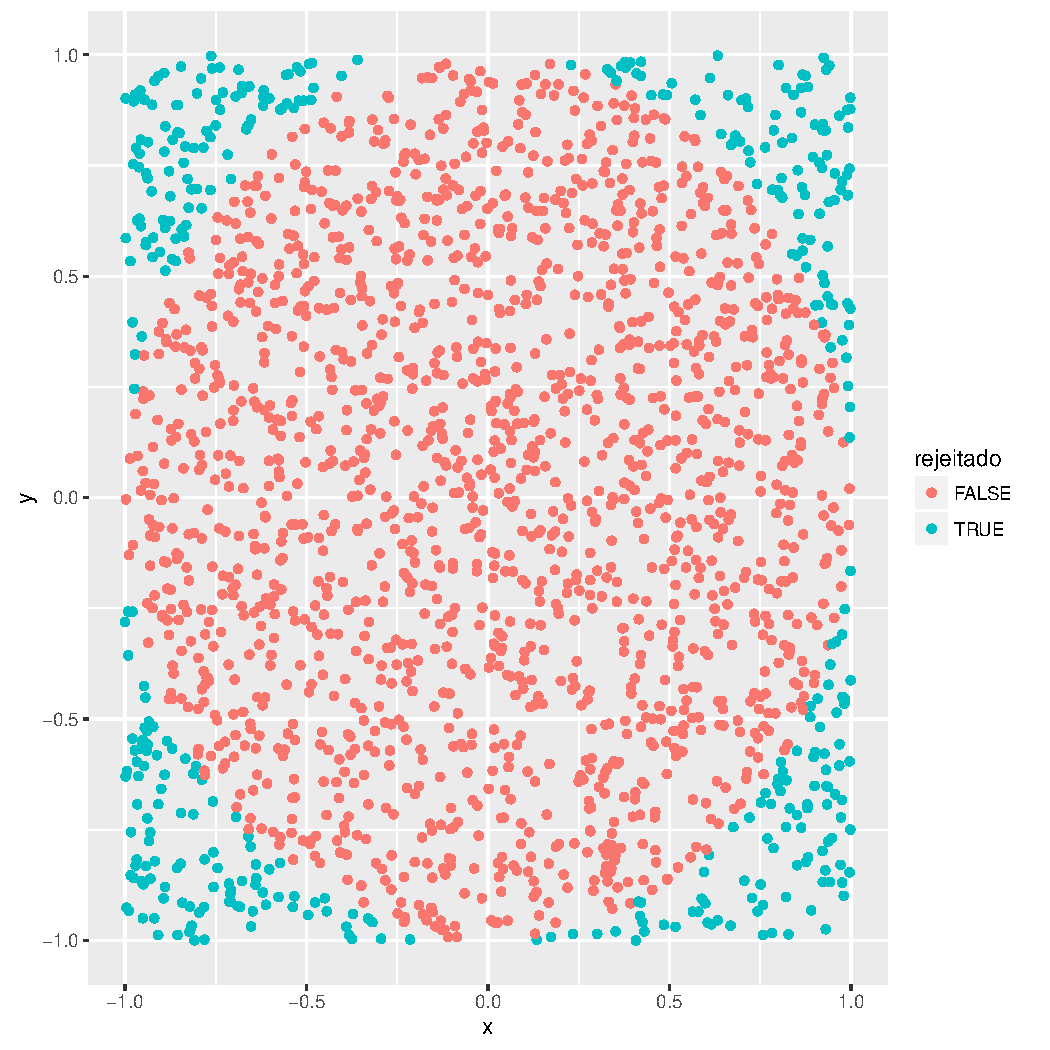
\includegraphics[scale=0.5]{chapter-computing-rejection-circle}
  \caption{Amostra de $2000$ propostas geradas pelo
  método da rejeição descrito
  no \cref{ex:rejection-circle}.}
  \label{fig:rejection-circle}
 \end{figure}
\end{example}

\begin{example}
 \label{ex:rejection-beta-2-2}
 Você deseja simular da densidade
 $f(\theta) = 6\theta(1-\theta)\I(\theta \in (0,1))$.
 Note que $f(\theta)$ é a densidade da Beta$(2,2)$.
 Podemos tomar, por exemplo,
 $\tilde{f}(\theta) = \theta(1-\theta) \I(\theta \in (0,1))$.
 Assim, $\tilde{f}(\theta) \leq 0.25 \I(\theta \in (0,1)) = 0.25 \cdot h(\theta)$,
 onde $h(\theta)$ é a densidade da
 Uniforme$(0,1)$ e $M=0.25$.
 Note que $\frac{\tilde{f}(\theta)}{M h(\theta)} = 4\theta(1-\theta)$.
 Portanto, é possível simular de $f$ pelo
 método da rejeição 
 usando o seguinte código
 \begin{verbatim}
###############################################################
## retorna: uma variável aleatória de distribuição Beta(2,2) ##
###############################################################
simula_beta_2_2_rejeicao <- function(B)
{
 amostra <- vector(mode="list", length=B)
 for(ii in 1:B)
 {
  T <- runif(1)
  while(runif(1) > 4*T*(1-T)) T <- runif(1)
  amostra[[ii]] <- T
 }
 return(amostra)
}
\end{verbatim}

 O funcionamento do algoritmo acima é ilustrado na
 \cref{fig:rejection-beta-2-2}.
 O eixo $x$ dos pontos indicam as $2000$ propostas que
 foram geradas para obter uma amostra de tamanho $1315$.
 O eixo $y$ dos pontos indicam as
 variáveis aleatórias uniformes geradas para
 determinar se as propostas eram rejeitadas.
 Dentre os pontos gerados, os vermelhos foram aceitos e
 os azuis foram rejeitados.
 Note que, como $\frac{\tilde{f}(\theta)}{h(\theta)} = 4\theta(1-\theta)$,
 $T$ era rejeitado se $U > 4T(1-T)$.
 A \cref{fig:rejection-beta-2-2} também ilustra um
 outro aspecto do método da rejeição.
 Ao combinarmos $T$ e $U$, obtemos uma
 distribuição uniforme em $[0,1]^{2}$.
 Ao remover os pontos azuis,
 os pontos vermelhos que restam distribuem-se de
 acordo com uma distribuição Beta(2,2) no eixo $x$.
 \begin{figure}
  \centering
  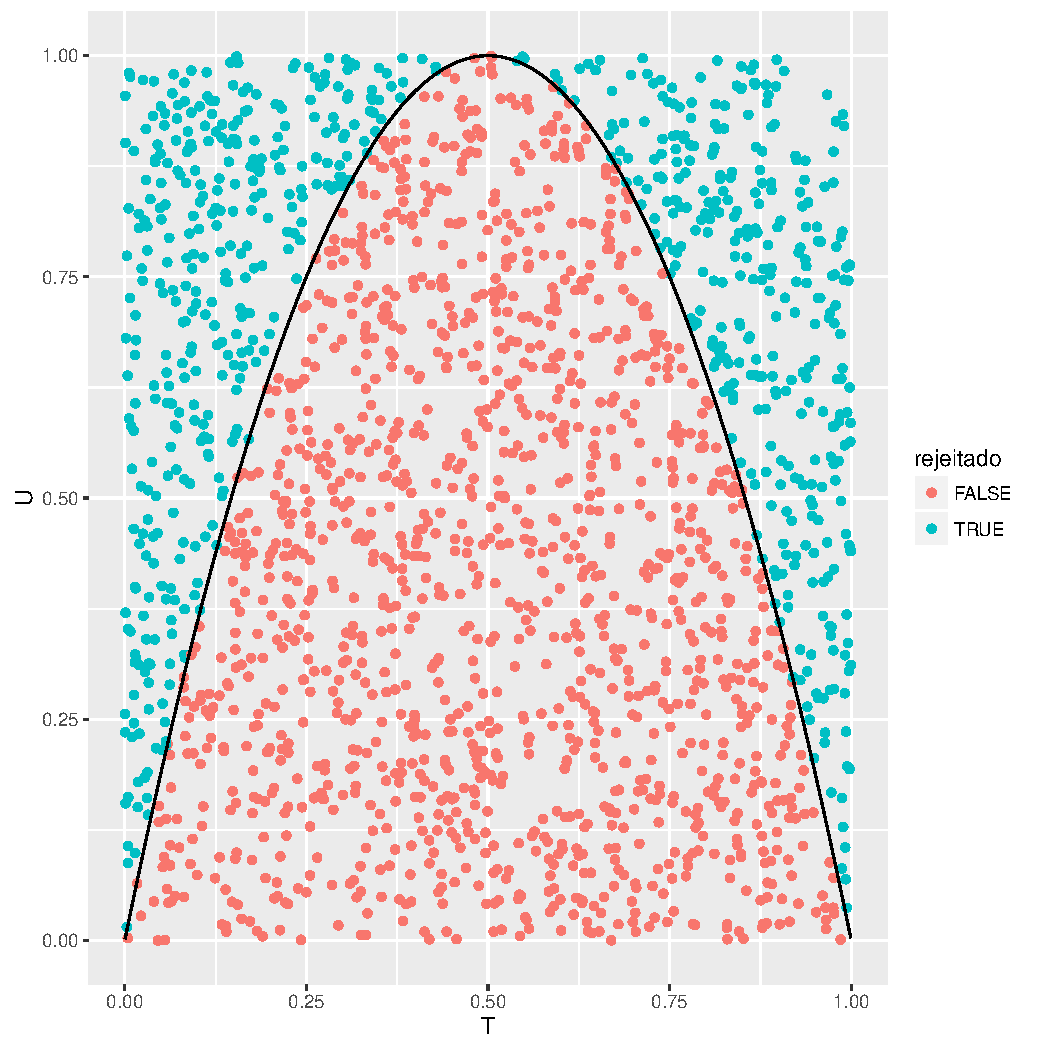
\includegraphics[scale=0.5]{chapter-computing-rejection-beta-2-2}
  \caption{Amostra de $2000$ propostas geradas pelo
  método da rejeição descrito no
  \cref{ex:rejection-beta-2-2}.}
  \label{fig:rejection-beta-2-2}
 \end{figure}
\end{example}

\begin{theorem}
 Se $\theta$ foi gerado de acordo com o
 método da rejeição usando as funções $f(\theta)$,
 $\tilde{f}(\theta)$, $h(\theta)$ e $M$
 conforme a descrição no início deste capítulo,
 então $\theta$ tem distribuição com densidade $f$.
\end{theorem}

\begin{proof}
 Considere que $N$ é o número de propostas geradas
 até a primeira aceitação, que
 $T_{1},\ldots,T_{i},\ldots$ é um conjunto de propostas e
 $U_{1},\ldots,U_{i},\ldots$ é um conjunto de uniformes.
 Note que $A_{i} = \I\left(U_{i} \leq \frac{\tilde{f}(T_{i})}{Mh(T_{i})}\right)$ são i.i.d. e
 \begin{align*}
  \P\left(U_{i} \leq
  \frac{\tilde{f}(T_{i})}
  {Mh(T_{i})}\right)
  &= \int_{-\infty}^{\infty}
  {\frac{\tilde{f}(t)}{Mh(t)} h(t) dt} \\
  &= M^{-1}\int_{-\infty}^{\infty}
  {\tilde{f}(t)dt} := p_{1}
 \end{align*}
 Portanto, como $N = \min\left(i: \I(U_{i} \leq \frac{\tilde{f}(T_{i})}{Mh(T_{i})}) =1\right)$,
 então $N \sim \text{Geométrica}(p_{1})$. Assim, para todo 
 $B \subset \mathbb{R}$,
 \begin{align*}
  \P(\theta \in B)
  &= \sum_{n}{\P(\theta \in B, N = n)} \\
  &= \sum_{n}{\P(\cap_{i=1}^{n-1}{A_{i}^{c}} \cap (A_{n} \cap T_{n} \in B))} \\
  &= \sum_{n}{\P(\cap_{i=1}^{n-1}{A_{i}^{c}})\P(A_{n} \cap T_{n} \in B)} \\
  &= \sum_{n}{(1-p_{1})^{n-1}\int_{B}{\frac{\tilde{f}(t)}{Mh(t)} h(t)dt}} \\
  &= \int_{B}{M^{-1}\tilde{f}(t)dt}\sum_{n}{(1-p_{1})^{n-1}} \\
  &= \frac{\int_{B}{M^{-1}\tilde{f}(t)dt}}{p_{1}} \\
  &= \frac{M^{-1}\int_{B}{\tilde{f}(t)dt}}{M^{-1}\int_{-\infty}^{\infty}{\tilde{f}(t)dt}} \\
  &= \int_{B}{\frac{\tilde{f}(t)}{\int_{-\infty}^{\infty}{\tilde{f}(t)dt}}dt} \\
  &= \int_{B}{f(t)dt}
 \end{align*} 
\end{proof}

\subsubsection*{Exercícios}

\begin{exercise}
 No \cref{ex:rejection-circle},
 usamos propostas de um quadrado de lado $2$
 e centro na origem.
 Poderíamos ter implementado o algoritmo da rejeição
 usando propostas de um quadrado de lado $1$?
 E de um quadrado de lado $3$?
 Esboce estas três figuras acompanhadas
 do círculo de raio $1$ e centro na origem.
 Compare as propostas sugeridas em relação à sua eficiência computacional.
\end{exercise}

\solution{\textbf{Solução}: A densidade de uma
 distribuição uniforme no quadrado de lado $1$ e
 centro na origem é,
 $h_{1}(\theta) := \I(|\theta_{1}| \leq 0.5, |\theta_{2}| \leq 0.5)$.
 Se tomarmos $f(\theta)$ como a densidade da
 distribuição uniforme no círculo de raio $1$ e
 centro na origem, então $f((1,0)) = 1$ e
 $h_{1}((1,0))$. Portanto, não existe $M > 0$ tal que
 $f((1,0)) \leq Mh_{1}((1,0))$.
														  Assim, não é possível usar o método da rejeição para  simular de $f$ a partir de $h_{1}$. 
 Por outro outro lado, defina
 $h_{2} = 4^{-1}\I(|\theta_{1}|\leq 1, |\theta_{2}|\leq 1)$ e $h_{3} = 9^{-1}\I(|\theta_{1}|\leq 1.5, |\theta_{2}|\leq 1.5)$ como as densidades dos quadrados
 de lado $2$ e $3$, e $\tilde{f}(\theta) = \I(\theta_{1}^{2}+\theta_{2}^{2} \leq 1)$.
 Note que $\tilde{f}(\theta) \leq 4 h_{2}$ e
 $\tilde{f}(\theta) \leq 9 h_{3}$.
 Assim, a probabilidade de aceitação usando
 $\tilde{f}$, $h_{2}$ e $M=4$ é dada por
 
 \begin{align*}
  \P\left(U \leq \frac{\tilde{f}(T)}{4 h_{2}(T)}\right)
  &= \int_{-\infty}^{\infty}{\frac{\tilde{f}(t)}{4 h_{2}(t)} h_{2}(t)dt} \\
  &= 4^{-1}\int_{-\infty}^{\infty}{\tilde{f}(t)dt}
  = \frac{\pi}{4}
 \end{align*}
 
 Similarmente, a probabilidade de aceitação usando
 $\tilde{f}$, $h_{3}$ e $M=9$ é $\frac{\pi}{9}$.
 Como a probabilidade de aceitação usando $h_{2}$ é
 maior do que usando $h_{3}$, o primeiro é
 mais computacionalmente eficiente.
 
 Este argumento é ilustrado pela
 \cref{fig:rejection-squares}.
 Note que a região de rejeição usando
 $h_{3}$ (azul e verde) é consideravelmente maior
 que aquela usando $h_{2}$ (verde).
 \begin{figure}
  \centering
  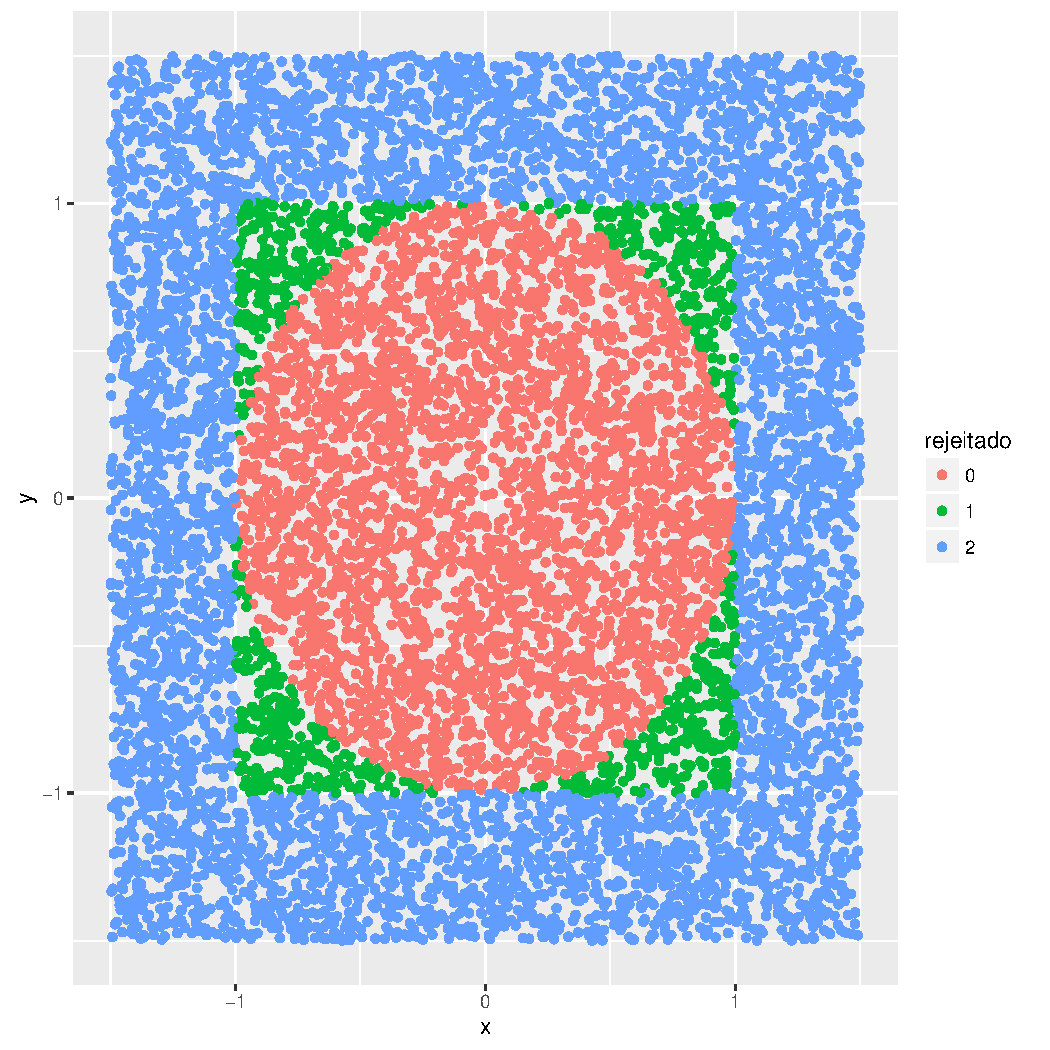
\includegraphics[scale=0.5]{chapter-computing-rejection-squares}
  \caption{Ilustração das regiões de rejeição
  para propostas de $h_{2}$ (verde) e de
  $h_{3}$ (verde e azul).}
  \label{fig:rejection-squares}
 \end{figure}
}{}

\begin{exercise}
 Escreva um código para
 simular da distribuição uniforme
 em uma esfera de raio $1$ e centro $0$.
 Use o Método de Monte Carlo para estimar
 a distância média de um ponto amostrado à origem.
\end{exercise}

\cprotect \solution{
 \textbf{Solução}: Podemos escolher
 $\tilde{f}(\theta) = \I(\theta_{1}^{2}+\theta_{2}^{2}+\theta_{3}^{2} \leq 1)$.
 Se usarmos como propostas a uniforme no cubo de
 aresta $1$ e centro na origem, então
 $h(\theta) = 8^{-1}\I(|\theta_{i}| \leq 1, i \in \{1,2,3\})$.
 Assim, $\tilde{f}(\theta) \leq 8h(\theta)$ e
 tomamos $M=8$.
 Neste caso, $\frac{\tilde{f}(\theta)}{8h(\theta)} = \tilde{f}(\theta)$.
 Portanto, o método da rejeição pode ser implementado
 da seguinte forma:
														
\begin{lstlisting}[language=R]
simula_esfera_rejeicao <- function(B) # retorna: pontos uniformemente
{                                     # da esfera de raio 1 centrada na origem.
 amostra <- vector(mode="list", length=B)
 for(ii in 1:B)
 {
  T <- runif(3,-1,1)
  while(sum(T^2) > 1) T <- runif(3,-1,1)
	amostra[[ii]] <- T
 }
 return(amostra)
}
\end{lstlisting}

Se usarmos o \cref{algo:monte_carlo}, obtemos

\begin{lstlisting}[language=R]
 B <- 10^4
 g <- function(coord) sqrt(sum(coord^2))
 monte_carlo(simula_esfera_rejeicao, B, g)
 
 estimador
 [1] 0.7484544
\end{lstlisting} 

 Note que a distância média de um ponto ao centro da
 esfera de raio $1$ é aproximadamente $0.75$.
 Assim, a distância média não é a metade do raio.
 Isto ocorre pois o volume da esfera a partir da
 metade do raio é maior do que o volume da esfera até
 a metade do raio.
}{}

\begin{exercise}
 \label{ex:circle-rejection-2}
 Escreva um código para
 simular de uma distribuição uniforme 
 em um círculo de raio $r$ e centro $c$.
 Qual é a relação entre o raio do círculo e a 
 distância média de um ponto amostrado ao seu centro?
 Exiba uma figura que ilustre essa relação.
\end{exercise}

\cprotect \solution{\textbf{Solução}: 
 Existem ao menos duas soluções para este problema.
 A primeira utiliza a simulação da distribuição uniforme
 no círculo de raio $1$ e centro na origem
 (\cref{ex:rejection-circle})
 para obter distribuições uniformes em outros círculos.
 Note que, se $\theta$ tem distribuição uniforme
 no círculo de raio $1$ e centro na origem,
 então $r \theta + c$ tem distribuição
 uniforme no círculo de raio $r$ e centro $c$.

 A segunda solução consiste em simular diretamente
 da distribuição uniforme no círculo de raio $r$ e
 centro $c$. Esta distribuição tem densidade
 $f(\theta) = \frac{1}{\pi r^{2}}\I((\theta_{1}-c_{1})^{2}+(\theta_{2}-c_{2})^{2} \leq r^{2})$.
 Portanto, podemos tomar
 $\tilde{f}(\theta) = \I((\theta_{1}-c_{1})^{2}+(\theta_{2}-c_{2})^{2} \leq r^{2})$.
 Para simular desta distribuição, podemos tomar o
 quadrado de lado $2r$ e centro em $c$.
 Assim, $h(\theta) = (2r)^{-2}\I(|\theta_{1}-c_{1}| \leq r, |\theta_{2}-c_{2}| \leq r)$.
 Portanto, $\tilde{f}(\theta) \leq (2r)^{2}h(\theta)$ e
 obtemos $\frac{\tilde{f}(\theta)}{(2r)^{2}h(\theta)} = \tilde{f}(\theta)$.
 Assim, é possível simular de $f$ pelo
 método da rejeição usando o seguinte código:

 \begin{lstlisting}[language=R]
simula_circulo_rejeicao <- function(B, centro, raio)
{
 amostra <- vector(mode="list", length=B)
 for(ii in 1:B)
 {
  T <- runif(2,-raio,raio)+centro
  while(sum(((T-centro)/raio)^2) > 1) T <- runif(2,-raio,raio)+centro
  amostra[[ii]] <- T
 }
 return(amostra)
}
 \end{lstlisting}

 Podemos obter estimadores das distâncias ao
 centro do círculo e exibi-los graficamente usando o
 seguinte código:

 \begin{lstlisting}[language=R]
 raios <- 1:10
 estimadores <- rep(NA, length(raios))
 g <- function(coord) sqrt(sum(coord^2))
 for(ii in 1:length(raios)) 
 {
  estimadores[ii] <- monte_carlo(simula_circulo_rejeicao, 10^3, g, 
                                 c(0,0), raios[ii])[["estimador"]]
 }
 dados <- data.frame(raio=raios, distancia=estimadores)
 ggplot(data=dados, aes(x=raio, y=distancia))+
 geom_point()+
 geom_smooth(method='lm',formula=y~x)
 \end{lstlisting}

O resultado é exibido na
\cref{fig:circle-rejection-2}.

\begin{figure}
 \centering
 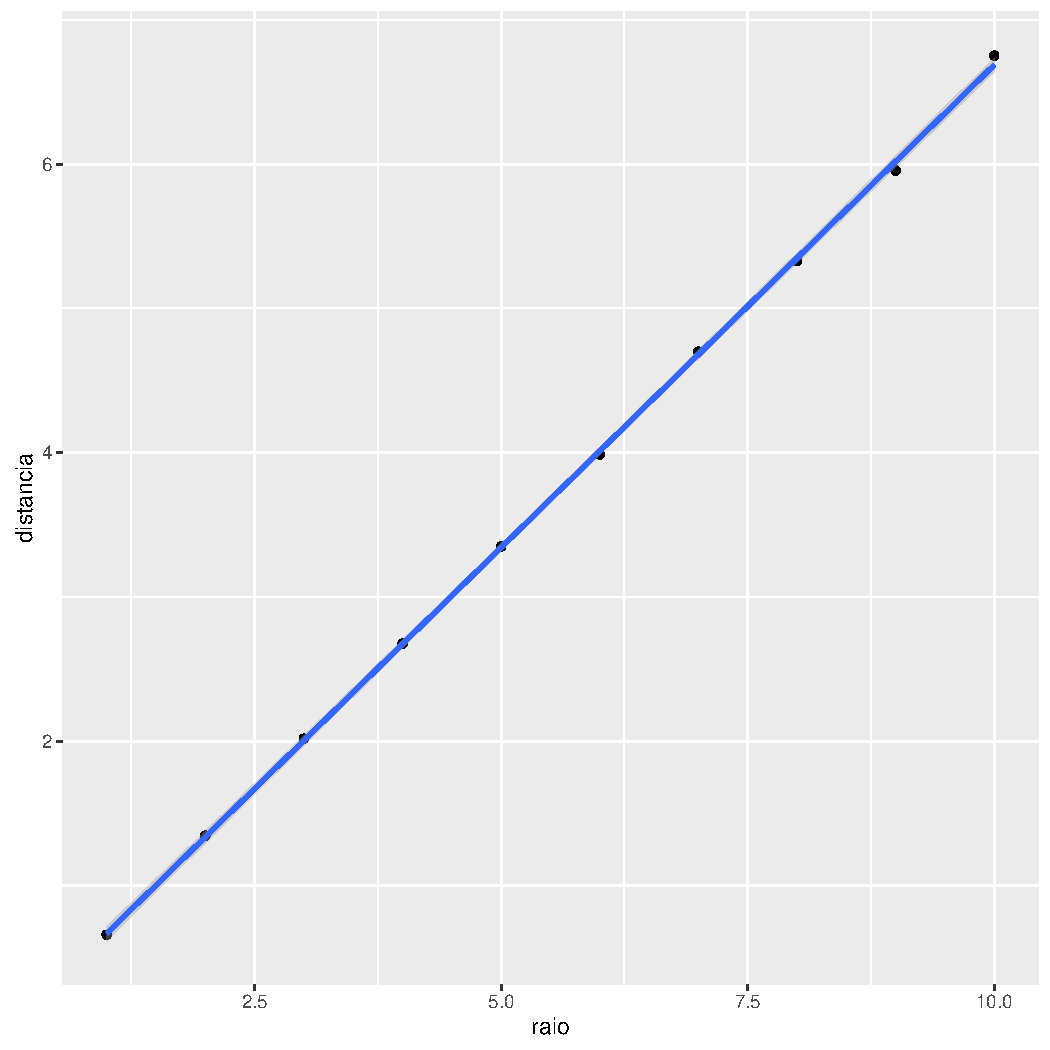
\includegraphics[scale=0.3]{chapter-computing-circle-distance}
 \caption{Variação linear da distância ao centro de
 acordo com o raio (\cref{ex:circle-rejection-2}).}
 \label{fig:circle-rejection-2}
\end{figure}
}{}

\begin{exercise}
 \label{ex:rejection-beta-a-b}
 Escreva código para
 simular de uma $\text{Beta}(a,b)$
 a partir de uma $\text{Uniforme}(0,1)$.
 Estime a média da $\text{Beta}(a,b)$ pelo
 método de Monte Carlo.
 Compare as taxas de rejeição do algoritmo proposto
 para alguns valores de $a$ e de $b$.
 Qual é a relação entre esses valores e
 a eficiência computacional do algoritmo proposto?
\end{exercise}

\cprotect \solution{\textbf{Solução}:
 O problema determina que
 $h(\theta) = \I(0 \leq \theta \leq 1)$.
 Podemos tomar $f(\theta) = \tilde{f}(\theta) = dbeta(\theta,a,b)$.
 Note que a moda da Beta$(a,b)$ é
 $\frac{a-1}{a+b-2}$. Portanto,
 $\tilde{f}(\theta) \leq \tilde{f}\left(\frac{a-1}{a+b-2}\right)h(\theta)$.
 Assim, as condições na amostragem por rejeição
 estão satisfeitas tomando
 $M= \tilde{f}\left(\frac{a-1}{a+b-2}\right)$.
 Portanto, podemos simular da Beta$(a,b)$ da
 seguinte forma
 \begin{lstlisting}[language=R]
simula_beta_rejeicao <- function(B,alpha,beta)
{
 M <- dbeta((alpha-1)/(alpha+beta-2),alpha,beta)
 amostra <- vector(mode="list", length=B)
 for(ii in 1:B)
 {
  T <- runif(1,0,1)
	rejeicoes <- 0
  while(runif(1,0,1) > dbeta(T,alpha,beta)/M) 
	{
	 T <- runif(1,0,1)
   rejeicoes <- rejeicoes+1
	}
	amostra[[ii]] <- c(T, rejeicoes)
 }
 return(amostra)
}
 \end{lstlisting} 

 Para entender de que forma o número de rejeições se
 comporta de acordo com $a$ e $b$, 
 geraremos amostradores para os casos em que $a=b$,
 para diversos valores de $a$ entre $2$ e $10$.
 O código está exibido abaixo.

 \begin{lstlisting}[language=R]
rejeicoes <- function(x) x[2]
param <- 2:10 
estimadores <- rep(NA, length(param))
for(ii in 1:length(param))
{
 estimadores[ii] <- monte_carlo(simula_beta_rejeicao, 10^4, rejeicoes, 
                                param[ii], param[ii])[["estimador"]]
}
dados <- data.frame(parametros=param, rejeicoes=estimadores)
ggplot(data=dados, aes(x=parametros, y=rejeicoes))+
geom_point()+
geom_smooth(method='lm',formula=y~x)
 \end{lstlisting}

 \begin{figure}
  \centering
  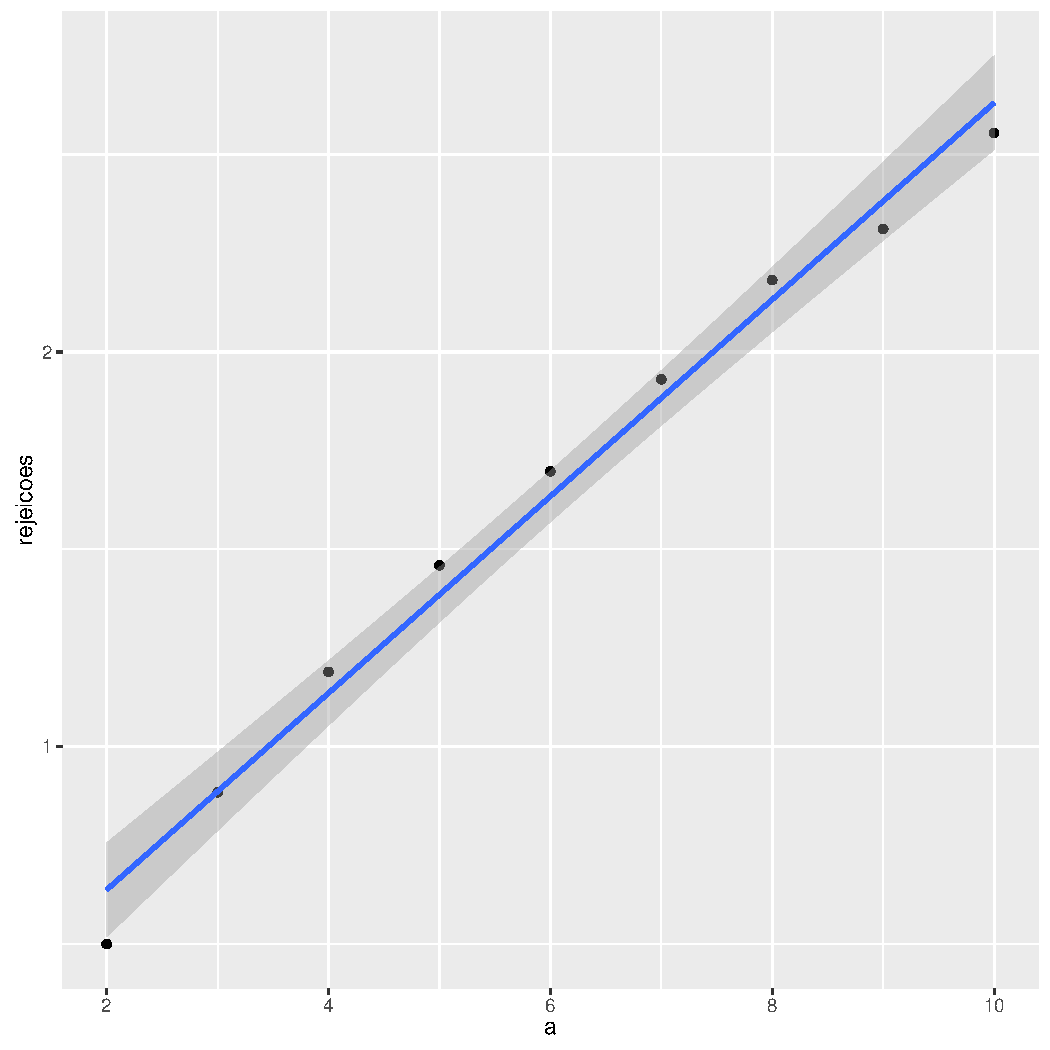
\includegraphics[scale=0.3]{chapter-computing-beta-rejections}
  \caption{Variação da taxa de rejeição
  de acordo com o valor de $a$
  (\cref{ex:rejection-beta-a-b}).}
  \label{fig:rejection-beta-a-b-1}
 \end{figure}

 A \cref{fig:rejection-beta-a-b-1} mostra que,
 quanto maiores os valores de $a$ e $b$, 
 maior a taxa de rejeição. 
 Isto ocorre pois a distribuição da Beta(a,b) 
 fica mais ``diferente'' da distribuição Uniforme(0,1)
 à medida que o valor de $a$ e $b$ aumentam.
 Este fato é ilustrado na
 \cref{fig:rejection-beta-a-b-2}.

 \begin{figure}
  \centering
  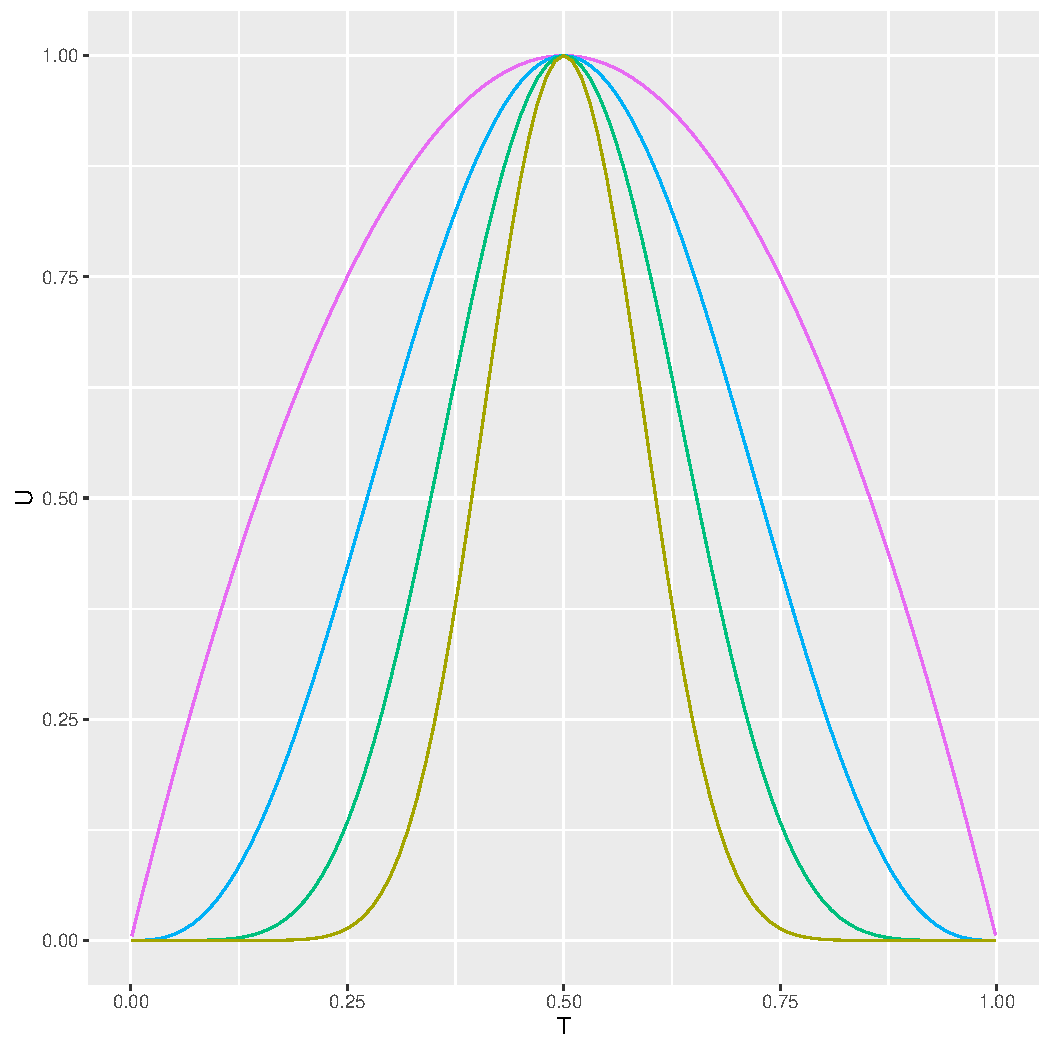
\includegraphics[scale=0.5]{chapter-computing-rejection-beta-a-b}
  \caption{Ilustração das regiões de rejeição
  para a Beta(2,2) (roxo), a Beta(4,4) (azul),
  a Beta(8,8) (verde) e a Beta(16,16) (marrom).}
  \label{fig:rejection-beta-a-b-2}
 \end{figure}
}{}

\begin{exercise}
 Sob quais condições é possível usar
 o método da rejeição para simular de
 uma $\text{Beta}(a,b)$ a partir de uma
 $\text{Beta}(a^{*},b^{*})$?
\end{exercise}

\cprotect \solution{\textbf{Solução}:
 Se $f(\theta) = dbeta(a,b)$ e
 $h(\theta) = dbeta(a^{*},b^{*})$, então
 \begin{align*}
  \frac{f(\theta)}{h(\theta)}
  &= \frac{Beta^{-1}(a,b)\theta^{a-1}(1-\theta)^{b-1}}{Beta^{-1}(a^{*},b^{*})\theta^{a^{*}-1}(1-\theta)^{b^{*}-1}} \\
  &= \frac{Beta(a^{*},b^{*})}
  {Beta(a,b)} \theta^{a-a^{*}}(1-\theta)^{b-b^{*}}
 \end{align*}
 Note que, se $a < a^{*}$, então
 $\frac{f(\theta)}{h(\theta)}$ pode ser
 arbitrariamente grande tomando-se $\theta \approx 0$.
 Similarmente, se $b < b^{*}$, então
 $\frac{f(\theta)}{h(\theta)}$ pode ser
 arbitrariamente grande tomando-se $\theta \approx 1$.
 Nestes casos, não existe $M$ tal que
 $f(\theta) \leq Mh(\theta)$.
 Portanto, se $a< a^{*}$ ou $b < b^{*}$,
 então não é possível amostrar de uma Beta$(a,b)$ 
 a partir de uma Beta$(a^{*},b^{*})$.

 Contudo, se $a>a^{*}$ e $b>b^{*}$,
 então $\frac{f(\theta)}{h(\theta)}$ é
 proporcional à densidade de uma
 Beta$(a-a^{*}+1,b-b^{*}+1)$.
 Portanto, $\frac{f(\theta)}{h(\theta)}$ tem
 seu valor maximizado em
 $\theta = \frac{a-a^{*}}{a-a^{*}+b-b^{*}}$.
 Assim, obtemos,
 \begin{align*}
  \frac{f(\theta)}{h(\theta)}
  &\leq \frac{Beta(a^{*},b^{*})}{Beta(a,b)} \left(\frac{a-a^{*}}{a-a^{*}+b-b^{*}}\right)^{a-a^{*}}\left(1-\frac{a-a^{*}}{a-a^{*}+b-b^{*}}\right)^{b-b^{*}} \\
  f(\theta) &\leq \frac{Beta(a^{*},b^{*})}{Beta(a,b)} \left(\frac{a-a^{*}}{a-a^{*}+b-b^{*}}\right)^{a-a^{*}}\left(1-\frac{a-a^{*}}{a-a^{*}+b-b^{*}}\right)^{b-b^{*}} h(\theta)
 \end{align*}
 Portanto, podemos tomar $\tilde{f}(\theta)=f(\theta)$ e
 $M=\frac{Beta(a^{*},b^{*})}{Beta(a,b)} \left(\frac{a-a^{*}}{a-a^{*}+b-b^{*}}\right)^{a-a^{*}}\left(1-\frac{a-a^{*}}{a-a^{*}+b-b^{*}}\right)^{b-b^{*}}$.
 
 Assim, obtemos o código:

 \begin{lstlisting}[language=R]
# retorna uma beta(a1, b1) pelo metodo da rejeicao
# por meio de uma beta(a2,b2)
simula_beta_via_beta <- function(B,a1,b1,a2,b2) {
 M <- ((a1-a2)/(a1-a2+b1-b2))^(a1-a2)*(1-(a1-a2)/(a1-a2+b1-b2))^(b1-b2)
 amostra <- vector(mode="list", length=B)
 for(ii in 1:B) {
  T <- rbeta(1,a2,b2)
  while(runif(1) > T^(a1-a2)*(1-T)^(b1-b2)/M)  T <- rbeta(1,a2,b2)
  amostra[[ii]] <- T
 }
 return(amostra)
}
 \end{lstlisting}
}{}

\begin{exercise}
 Sob quais condições é possível usar
 o método da rejeição para simular de uma
 $\text{Gama}(a,b)$ a partir de uma
 $\text{Exponencial}(c)$? Escreva o
 código para realizar esta simulação. 
\end{exercise}


\subsection{Método de Monte Carlo via cadeias de Markov}

Foi ilustrado na seção passada que
nem sempre é possível obter de forma eficiente
uma sequência de variáveis aleatórias i.i.d.
com distribuição dada pela posteriori. Assim,
a aplicação do método de Monte Carlo é
inviável. 

Para contornar este problema, esta seção
apresenta o método de Monte Carlo via
cadeias de Markov. Neste método, ao invés de
você gerar uma sequência i.i.d., você
gerará uma cadeia de Markov. 
A \cref{subsec:markov} revisa cadeias de Markov e
a \cref{subsec:mh} apresenta o algoritmo de
Metropolis-Hastings, uma implementação geral do
método de Monte Carlo via cadeias de Markov.

\subsubsection{Cadeias de Markov}
\label{subsec:markov}

\begin{definition}[Cadeia de Markov]
 Seja $(T_{n})_{n \in \mathbb{N}}$ uma
 sequência de variáveis discretas.
 Dizemos que $(T_{n})_{n \in \mathbb{N}}$ é
 uma Cadeia de Markov se,
 para todo $n \in \mathbb{N}$,
 \begin{align*}
  \P(T_{n+1}=t_{n+1}|T_{n}=t_{n}, T_{n-1}=t_{n-1},\ldots, T_{1}=t_{1}) 
  &= \P(T_{n+1}=t_{n+1}|T_{n}=t_{n})
 \end{align*}
\end{definition}
Isto é, dado o passado inteiro da cadeia de Markov, ($T_{n}=t_{n}, T_{n-1}=t_{n-1}, \ldots, T_{1}=t_{1}$),
apenas o estado imediatamente anterior,
$(T_{n}=t_{n})$, é usado para determinar o próximo estado $(T_{n+1})$.
      
\begin{definition}[Cadeia homogênea]
 Seja $(T_{n})_{n \in \mathbb{N}}$ uma 
 cadeia de Markov.  Dizemos que
 $(T_{n})_{n \in \mathbb{N}}$ é homogênea se,
 para todo $n$, $\P(T_{n+1}=t_{n+1}|T_{n}=t_{n}) = f(t_{n},t_{n+1})$. 
 Isto é, a distribuição do próximo estado da
 cadeia depende do estado anterior, mas não do
 índice atual. Neste caso, denotamos a função de
 transição da cadeia,  $\P(T_{n+1}=t_{n+1}|T_{n}=t_{n})$ por
 $p(t_{n+1}|t_{n})$.
 A partir deste ponto, consideraremos apenas
 cadeias de Markov homogêneas. 
\end{definition}

\begin{definition}[Matriz de transição]
 \label{defn:transition}
 Seja $(T_{n})_{n \in \mathbb{N}}$ uma
 cadeia de Markov homogênea. 
 $\P$ é a matriz de transição para
 $(T_{n})_{n \in \mathbb{N}}$ se 
 $\P_{i,j} = \P(T_{n+1}=j|T_{n}=i) = p(j|i)$. 
 Isto é, a intersecção entre a i-ésima linha de
 $\P$ e a j-ésima coluna contém a probabilidade de
 a cadeia ir do estado $i$ para o estado $j$. 
\end{definition}

\begin{example}
 \label{ex:0-1-chain}
 Considere uma cadeia de Markov em $\{0,1\}$ com
 a seguinte matriz de transição:
 \begin{align*}
  \P &= \left[
  \begin{array}{cc}
   \frac{1}{3} & \frac{2}{3} \\
   \frac{1}{2} & \frac{1}{2}
  \end{array} \right ]
 \end{align*}
 Isto é, $\P(T_{1}=0|T_{0}=0) = \frac{1}{3}$,
 $\P(T_{1}=1|T_{0}=0) = \frac{2}{3}$,
 $\P(T_{1}=0|T_{0}=1) = \frac{1}{2}$ e
 $\P(T_{1}=1|T_{0}=1) = \frac{1}{2}$. 
\end{example}
       
\begin{definition}[Distribuição estacionária]
 Seja $(T_{n})_{n \in \mathbb{N}}$ uma
 cadeia de Markov com matriz de transição, $\P$. 
 Para cada estado, $i$, definimos
 \begin{align*}
  \mu(i) = \limn \P(T_{n} = i|T_{0}=t_{0})
  = \limn (\P^n)_{t_{0},i}
 \end{align*}
 Se o limite for bem definido, dizemos que $\mu$ é a distribuição estacionária da Cadeia.
 Podemos interpretar $\mu(i)$ como a probabilidade de que, 
 após um tempo suficientemente grande ter se passado,
 a cadeia esteja no estado $i$. 
\end{definition}

A definição de distribuição estacionária envolve
um limite de multiplicações de matrizes.
Achar este limite por força bruta pode ser
muito difícil. Assim, a seguir, definimos uma
distribuição mais fácil de calcular e provamos que,
sob certas circunstâncias, ela é equivalente à
distribuição estacionária.

\begin{definition}[Distribuição invariante]
 \label{defn:invariant}
 Seja $(T_{n})_{n \in \mathbb{N}}$ uma
 cadeia de Markov com matriz de transição, $\P$. 
 Seja $\mu$ um vetor não-negativo tal que
 $\sum_{i}{\mu(i)} = 1$. 
 $\mu$ é a distribuição invariante para $\P$ se
 \begin{align*}
  \mu \P = \mu 
 \end{align*}
 Isto é, se a sua informação sobre o
 estado atual da cadeia é $\mu$, então sua
 informação para o próximo estado da cadeia
 também é $\mu$. Desta forma,
 $\mu$ é um ponto fixo de $\P$.
\end{definition}

\begin{example}
 Considere o \cref{ex:0-1-chain}.
 A distribuição invariante deve satisfazer:
 \begin{align*}
  \mu &=
  \mu \cdot \begin{bmatrix}
   \frac{1}{3} & \frac{2}{3} \\
   \frac{1}{2} & \frac{1}{2}
  \end{bmatrix}
 \end{align*}
 Do que obtemos o sistema linear:
 \begin{align*}
  \begin{cases}
   \frac{\mu(0)}{3}+\frac{\mu(1)}{2} = \mu(0) \\
   \frac{2\mu(0)}{3}+\frac{\mu(1)}{2} = \mu(1) \\
   \mu(0) + \mu(1) = 1
  \end{cases}
 \end{align*}
 Portanto, $\mu(0) = \frac{3}{7}$ e
 $\mu(1) = \frac{4}{7}$.
\end{example}
      

\begin{theorem}
 Seja $(T_{n})_{n \in \mathbb{N}}$ uma
 cadeia de Markov de matriz de transição $\P$. 
 Sob algumas condições fracas de regularidade
 sobre $\P$, se $\mu$ é a
 distribuição invariante para $\P$, então
 $\mu$ é a distribuição estacionária para
 $\P$.
\end{theorem}

Muitas vezes, uma medida invariante
pode ser encontrada mais facilmente através de uma 
distribuição reversível:
      
\begin{definition}[Distribuição reversível]
 \label{defn:reversible}
 Seja $(T_{n})_{n \in \mathbb{N}}$ uma
 cadeia de Markov com
 matriz de transição $\P$. 
 Seja $\mu$ um vetor positivo tal que
 $\sum_{i}{\mu(i)} = 1$. 
 $\mu$ é a distribuição reversível para
 $\P$ se,  para todos estados $i$ e $j$,
 $\mu(i)\P_{i,j} = \mu(j)\P_{j,i}$. 
\end{definition}
      
\begin{example}
 Considere o \cref{ex:0-1-chain}. 
 Seja $\mu(0) = \frac{3}{7}$ e
 $\mu(1) = \frac{4}{7}$.
 \begin{align*}
  \mu(0) \P_{0,1}
  &= \frac{3}{7} \cdot \frac{2}{3}
  = \frac{2}{7} \\
  &= \frac{4}{7} \cdot \frac{1}{2}
  = \mu(1)\P_{1,0}
 \end{align*}
 Portanto, $\mu$ é reversível.
\end{example}
      
\begin{lemma}
 \label{reversibility-implies-invariance}
 Se $\mu$ é a distribuição reversível para $\P$, 
 então $\mu$ é a distribuição invariante para $\P$. 
\end{lemma}
 
\begin{proof}
 Considere que $\mu$ é a distribuição reversível
 para $\P$. Portanto, para todo $j$,
 \begin{align*}
  (\mu \P)_{j}
  &= \sum_{i}{\mu(i)\P(i,j)} \\
  &= \sum_{i}{\mu(j)\P(j,i)}
  & \text{\cref{defn:reversible}} \\
  &= \mu(j)\sum_{i}{\P(j,i)} \\
  &= \mu(j)
  & \text{\cref{defn:transition}}
 \end{align*}
 Isto é, para todo j, $(\mu \P)_{j} = \mu(j)$.
 Conclua que $\mu \P = \mu$, ou seja,
 $\mu$ é a distribuição invariante
 (\cref{defn:invariant}).
\end{proof}

\begin{example}
 Seja $(T_{n})_{n \in \mathbb{N}}$ uma 
 cadeia de Markov de matriz de transição $\P$. 
 Considere, para quaisquer estados $i$ e $j$, 
 $\P_{i,j} = \P_{j,i}$. 
 Defina $\mu(i) = \frac{1}{N}$, onde
 $N$ é o número total de estados.
 Observe que $\sum_{i}{\mu(i)} = 1$ e também,
 \begin{align*}
  \mu(i) \P_{i,j}
  &= \frac{1}{N} \cdot \P_{i,j} \\
  &= \frac{1}{N} \cdot \P_{j,i}
  = \mu(j) \P_{j,i}
 \end{align*}
 Portanto $\mu$ é reversível.
 Decorre do \cref{reversibility-implies-invariance}
 que $\mu$ é invariante. 
 Portanto, sob a condição de que $\mathbb{P}_{i,j} = \mathbb{P}_{j,i}$,
 a distribuição uniforme é invariante. 
\end{example}

\begin{theorem}[Lei dos grandes números e Teorema do limite central para cadeias de Markov {\citep{Jones2004}}]
 \label{theorem:clt-markov}
 Seja $(T_{n})_{n \in \mathbb{N}}$ uma 
 cadeia de Markov,
 $\mu$ a distribuição estacionária de
 $(T_{n})_{n \in \mathbb{N}}$ e 
 $g$ uma função contínua.
 Sob algumas condições fracas de regularidade,
 \begin{align*}
  \frac{\sum_{i=1}^{B}{g(T_{i})}}{B}
  &\approx \E_{\mu}[g(T)]
  = \int{g(\theta)\mu(\theta)d\theta} \\
  \V\left[\frac{\sum_{i=1}^{B}{g(T_{i})}}{B}\right] 
  &\approx \frac{\V[g(T_{i})]+2\sum_{k=1}^{\infty}{Cov[g(T_{i}),g(T_{i+k})]}}{B} \\
  \frac{\frac{\sum_{i=1}^{B}{g(T_{i})-E_{\mu}[g(T)]}}{B}}{\sqrt{Var\left[\frac{\sum_{i=1}^{B}{g(T_{i})}}{B}\right]}} &\approx N(0,1)
 \end{align*}
 Portanto,
 \begin{align*}
  \left[\frac{\sum_{i=1}^{B}{g(T_{i})}}{B}+\psi^{-1}(\alpha/2)\sqrt{\V\left[\frac{\sum_{i=1}^{B}{g(T_{i})}}{B}\right]},\frac{\sum_{i=1}^{B}{g(T_{i})}}{B}-\psi^{-1}(\alpha/2)\sqrt{\V\left[\frac{\sum_{i=1}^{B}{g(T_{i})}}{B}\right]}\right]
 \end{align*}
 É um intervalo de confiança $1-\alpha$ para
 $\int{g(\theta)\mu(\theta)d\theta}$.
\end{theorem}

\subsubsection{O algoritmo de Metropolis-Hastings}
\label{subsec:mh}

O \cref{theorem:clt-markov} mostra que,
se você construir uma cadeia de Markov, $T_{1},\ldots,T_{B}$,
com distribuição estacionária $f(\theta|x)$,
então $\frac{\sum_{i=1}^{B}{g(T_{i})}}{B}$ é um
estimador consistente para
$\int{g(\theta)f(\theta|x)d\theta} = \E[g(\theta)|X]$.
O \cref{theorem:clt-markov} também permite que 
você avalie a margem de erro para
esse estimador a partir
de $\V\left[\frac{\sum_{i=1}^{B}{g(T_{i})}}{B}\right]$.
Assim, se você obtiver uma cadeia de Markov com 
distribuição invariante igual à posteriori,
$f(\theta|x)$, então
poderá fazer Inferência Estatística.
Nesta subseção, veremos como obter esta cadeia.

Para tal, considere o algoritmo de
Metropolis-Hastings, descrito a seguir:

\begin{algorithm2}[Metropolis-Hastings] \
 \label{alg:m-h}
 \begin{enumerate}
  \item Defina um valor arbitrário para $T_{1}$.
  \item Para $i$ de $2$ até $B$:
  \begin{enumerate}[label=\alph*.]
   \item Obtenha $T_{i}^{*}$ da distribuição
   $h(t_{i}^*|T_{i-1})$,
   $h$ é uma distribuição condicional arbitrária.
   \item Obtenha $R_i=\frac{f(\theta=T_i^{*}|x)h(T_{i-1}|T_{i}^*)}{f(\theta=T_{i-1}|x)h(T_{i}^*|T_{i-1})}$.
   \item Gere $U_i \sim \text{Uniforme}(0,1)$.
   \item Defina:
   \begin{align*}
    T_{i} &=
    \begin{cases}
     T_{i}^{*} & \text{, se } U_i \leq R_i \\
     T_{i-1} & \text{, caso contrário.}
    \end{cases}
   \end{align*}
  \end{enumerate}
 \end{enumerate}
\end{algorithm2}

Em primeiro lugar, note que, para obter $R_i$,
utiliza-se $f(\theta|x)$. Contudo, você está estudando
métodos computacionais justamente por não ser
possível calcular a posteriori analiticamente.
Assim, poderá parecer que o algoritmo acima não é
operacional. Contudo, observe que:

\begin{align}
 \label{eq:m-h-2}
 R_i &=\frac{f(\theta=T_i^{*}|x)h(T_{i-1}|T_{i}^*)}
 {f(\theta=T_{i-1}|x)h(T_{i}^*|T_{i-1})} \nonumber \\
 &=\frac{\frac{f(\theta=T_i^{*})f(x|\theta=T_i^*)}{f(x)}h(T_{i-1}|T_{i}^*)}{\frac{f(\theta=T_{i-1})f(x|\theta=T_{i-1})}{f(x)}h(T_{i}^*|T_{i-1})} \nonumber \\
 &= \frac{f(\theta=T_i^{*})f(x|\theta=T_i^*)h(T_{i-1}|T_{i}^*)}{f(\theta=T_{i-1})f(x|\theta=T_{i-1})h(T_{i}^*|T_{i-1})}
\end{align}

Assim, uma vez que $R_i$ envolve uma razão de
posterioris, é possível calculá-lo utilizando
$f(\theta)f(x|\theta)$ ao invés de $f(\theta|x)$.
Em geral, enquanto que é possível obter a primeira quantidade analiticamente, não é possível obter a segunda. Assim, calcular $R_i$ a partir da 
\cref{eq:m-h-2} torna o algoritmo operacional.

Também note que, a cada iteração, $T_i$ é gerado
utilizando-se apenas as variáveis aleatórias
$T_{i-1}$ e $U_{i}$. Assim,
$T_{1},\ldots,T_{B}$ é uma cadeia de Markov.
Além disso, você também pode demonstrar que
$f(\theta|x)$ é a distribuição invariante 
desta cadeia.
Para tal, mostrará primeiro que 
$f(\theta|x)$ é a distribuição reversível de
$T_{1},\ldots,T_{B}$.

\begin{lemma}
 \label{lemma:mh-reversible}
 $f(\theta|x)$ é a distribuição reversível para
 a cadeia de Markov gerada pelo \cref{alg:m-h}.
\end{lemma}

\begin{proof}
 Para quaisquer estados, $a$ e $b$,
 \begin{align}
  \label{eq:m-h-1}
  f(\theta=a|x)f(T_{i}=b|T_{i-1}=a)
  &= f(\theta=a|x)f(T^{*}_i=b|T_{i-1}=a)
  f(T_{i}=b|T^{*}_{i}=b,T_{i-1}=a) \nonumber \\
  &= f(\theta=a|x)h(b|a)
  f\left(U_i \leq \frac{f(\theta=b|x)h(a|b)}
  {f(\theta=a|x)h(b|a)}\right) \nonumber \\
  &= f(\theta=a|x)h(b|a)
  \min\left(1,\frac{f(\theta=b|x)h(a|b)}
  {f(\theta=a|x)h(b|a)}\right)
 \end{align}
 Note que, se $\frac{f(\theta=b|x)h(a|b)}{f(\theta=a|x)h(b|a)}=1$, então:
 \begin{align*}
  f(\theta=a|x)f(T_{i}=b|T_{i-1}=a) &=
  f(\theta=a|x)h(b|a)
  & \text{\cref{eq:m-h-1}},
  \frac{f(\theta=b|x)h(a|b)}{f(\theta=a|x)h(b|a)}=1\\
  &= f(\theta=b|x)h(a|b)
  &\frac{f(\theta=b|x)h(a|b)}{f(\theta=a|x)h(b|a)}=1\\
  &= f(\theta=b|x)f(T_{i}=a|T_{i-1}=b)
  & \text{\cref{eq:m-h-1}},
  \frac{f(\theta=b|x)h(a|b)}{f(\theta=a|x)h(b|a)}=1
 \end{align*}
 Agora, sem perda de generalidade, suponha que
 $\frac{f(\theta=b|x)h(a|b)}{f(\theta=a|x)h(b|a)}<1$.
 Neste caso,
 \begin{align*}
  f(\theta=a|x)f(T_{i}=b|T_{i-1}=a) &=
  f(\theta=a|x)h(b|a)
  \frac{f(\theta=b|x)h(a|b)}
  {f(\theta=a|x)h(b|a)}
  & \text{\cref{eq:m-h-1}},
  \frac{f(\theta=b|x)h(a|b)}{f(\theta=a|x)h(b|a)}<1\\
  &= f(\theta=b|x)h(a|b) \\
  &= f(\theta=b|x)h(a|b)
  \min\left(1,\frac{f(\theta=a|x)h(b|a)}
  {f(\theta=b|x)h(a|b)}\right)
  &\frac{f(\theta=a|x)h(b|a)}{f(\theta=b|x)h(a|b)}>1\\
  &=f(\theta=b|x)f(T_i=a|T_{i-1}=b)
  & \text{\cref{eq:m-h-1}}
 \end{align*}
 Assim, usando a \cref{defn:reversible},
 conclua dos dois casos anteriormente
 analisados que $f(\theta|x)$ é a 
 distribuição reversível para a cadeia de Markov
 gerada pelo \cref{alg:m-h}.
\end{proof}

\begin{theorem}
 \label{thm:mh-invariant}
 $f(\theta|x)$ é a distribuição invariante para
 a cadeia de Markov gerada pelo \cref{alg:m-h}.
\end{theorem}

\begin{proof}
 Decorre dos \cref{reversibility-implies-invariance,lemma:mh-reversible}.
\end{proof}

Como resultado do \cref{thm:mh-invariant}, 
você obteve que o \cref{alg:m-h} gera uma
cadeia de Markov, $T_{1},\ldots,T_{B}$, de 
medida invariante $f(\theta|x)$.
Portanto, utilizando o \cref{theorem:clt-markov}, 
você pode utilizar $T_{1},\ldots,T_{B}$ para
aproximar $\E[g(\theta)|x]$, para
qualquer $g$ contínua.
Assim, você pode resolver problemas de Inferência,
ainda que não consiga calcular a
posteriori analiticamente.
O \cref{ex:m-h-r}, a seguir, ilustra uma
implementação genérica do \cref{alg:m-h} no R.
Vários exemplos a seguir utilizam esta
implementação para ilustrar o funcionamento do
\cref{alg:m-h}.

\begin{example}[Implementação genérica do \cref{alg:m-h} no R] \
 \label{ex:m-h-r}
\begin{knitrout}
\definecolor{shadecolor}{rgb}{0.969, 0.969, 0.969}\color{fgcolor}\begin{kframe}
\begin{alltt}
\hlcom{####################################################################################}
\hlcom{## retorna: um vetor que forma uma cadeia de Markov.                              ##}
\hlcom{## B: o tamanho da cadeia retornada.                                              ##}
\hlcom{## inicio: a posicao inicial da cadeia retornada.                                 ##}
\hlcom{## rprop: uma funcao que recebe como argumento elementos da cadeia e retorna uma  ##}
\hlcom{## proposta gerada a partir deste elemento                                        ##}
\hlcom{## ldprop: o log da densidade condicional da proposta utilizada.                  ##}
\hlcom{## ldpost: o log de uma funcão proporcional à                                     ## }
\hlcom{## densidade correspondente à distribuição invariante da cadeia gerada.           ##}
\hlcom{####################################################################################}
\hlstd{metropolis} \hlkwb{<-} \hlkwa{function}\hlstd{(}\hlkwc{B}\hlstd{,} \hlkwc{start}\hlstd{,} \hlkwc{rprop}\hlstd{,} \hlkwc{ldprop}\hlstd{,} \hlkwc{ldtgt}\hlstd{)}
\hlstd{\{}
  \hlstd{chain} \hlkwb{<-} \hlkwd{as.list}\hlstd{(}\hlkwd{rep}\hlstd{(}\hlnum{NA}\hlstd{, B))}
  \hlstd{chain[[}\hlnum{1}\hlstd{]]} \hlkwb{<-} \hlstd{start}
  \hlkwa{for}\hlstd{(ii} \hlkwa{in} \hlnum{2}\hlopt{:}\hlstd{B)}
  \hlstd{\{}
    \hlstd{prop} \hlkwb{<-} \hlkwd{rprop}\hlstd{(chain[[ii}\hlopt{-}\hlnum{1}\hlstd{]])}
    \hlstd{lratio} \hlkwb{<-} \hlkwd{ldtgt}\hlstd{(prop)}\hlopt{-}\hlkwd{ldtgt}\hlstd{(chain[[ii}\hlopt{-}\hlnum{1}\hlstd{]])}\hlopt{+}
              \hlkwd{ldprop}\hlstd{(prop,chain[[ii}\hlopt{-}\hlnum{1}\hlstd{]])}\hlopt{-}
              \hlkwd{ldprop}\hlstd{(chain[[ii}\hlopt{-}\hlnum{1}\hlstd{]],prop)}
    \hlkwa{if}\hlstd{(}\hlkwd{log}\hlstd{(}\hlkwd{runif}\hlstd{(}\hlnum{1}\hlstd{))} \hlopt{<=} \hlstd{lratio) chain[[ii]]} \hlkwb{<-} \hlstd{prop}
    \hlkwa{else} \hlstd{chain[[ii]]} \hlkwb{<-} \hlstd{chain[[ii}\hlopt{-}\hlnum{1}\hlstd{]]}
  \hlstd{\}}
  \hlkwd{return}\hlstd{(chain)}
\hlstd{\}}
\end{alltt}
\end{kframe}
\end{knitrout}
\end{example}

\begin{example}
 Digamos que $\mu \sim \text{T}_{1}$,
 isto é, uma distribuição $T$ com 1 grau de liberdade
 (também conhecida como distribuição Cauchy).
 Também, dado $\mu$, $X_1,\ldots,X_n$ são i.i.d.
 e $X_1 \sim N(\mu,1)$.
 Você deseja estimar $\mu$ minimizando a 
 perda quadrática. Note que:
 \begin{align*}
  f(\mu|\x)
  &= f(\mu)f(\x|\mu)
  = f(\mu)\prod_{i=1}^{n}{f(x_i|\mu)} \\
  &\propto f(\mu)\prod_{i=1}^{n}{\exp\left(-\frac{(x_i-\mu)^2}{2}\right)} \\
  &= f(\mu){\exp\left(-\sum_{i=1}^{n}{\frac{(x_i-\mu)^2}{2}}\right)} \\
  &= f(\mu)\exp\left(-\sum_{i=1}^{n}{\frac{(x_i-\bar{x})^2}{2}}-\frac{n(\bar{x}-\mu)^2}{2}\right) \\
  &\propto f(\mu)\exp\left(-\frac{n(\bar{x}-\mu)^2}{2}\right)
 \end{align*}
 Portanto, existe uma função proporcional a
 $f(\mu|x)$, $\tilde{f}(\mu|x)$, tal que
 \begin{align*}
  \log(\tilde{f}(\mu|\x))
  &= \log(f(\mu))-\frac{n(\bar{x}-\mu)^2}{2}
 \end{align*}
 Digamos que você observou uma amostra de
 tamanho $100$ e $\bar{x}=3.14$.
 Assim, pode implementar uma das
 entradas do \cref{ex:m-h-r} como:
\begin{knitrout}
\definecolor{shadecolor}{rgb}{0.969, 0.969, 0.969}\color{fgcolor}\begin{kframe}
\begin{alltt}
\hlstd{ldpost} \hlkwb{<-} \hlkwa{function}\hlstd{(}\hlkwc{mu}\hlstd{)} \hlkwd{log}\hlstd{(}\hlkwd{dt}\hlstd{(mu,}\hlkwc{df}\hlstd{=}\hlnum{1}\hlstd{))}\hlopt{-}\hlstd{(}\hlnum{100}\hlopt{*}\hlstd{(}\hlnum{3.14}\hlopt{-}\hlstd{mu)}\hlopt{^}\hlnum{2}\hlstd{)}\hlopt{/}\hlnum{2}
\end{alltt}
\end{kframe}
\end{knitrout}
Existe uma variedade enorme de propostas que
você pode utilizar. Uma possibilidade é
sugerir como proposta a observação anterior
somada a ruído branco. Neste caso, obtenha,
\begin{knitrout}
\definecolor{shadecolor}{rgb}{0.969, 0.969, 0.969}\color{fgcolor}\begin{kframe}
\begin{alltt}
\hlstd{rprop} \hlkwb{<-} \hlkwa{function}\hlstd{(}\hlkwc{ant}\hlstd{) ant}\hlopt{+}\hlkwd{rnorm}\hlstd{(}\hlnum{1}\hlstd{)}
\hlstd{ldprop} \hlkwb{<-} \hlkwa{function}\hlstd{(}\hlkwc{ant}\hlstd{,}\hlkwc{prop}\hlstd{)} \hlkwd{log}\hlstd{(}\hlkwd{dnorm}\hlstd{(prop,}\hlkwc{mean}\hlstd{=ant))}
\end{alltt}
\end{kframe}
\end{knitrout}
Dado que você está usando a perda quadrática,
o estimador ótimo é $\E[\theta|x]$.
Decorre do \cref{theorem:clt-markov} que
você pode aproximar esta quantidade por
$\frac{\sum_{i=1}^{n}{T_{i}}}{B}$, que é
obtida por
\begin{knitrout}
\definecolor{shadecolor}{rgb}{0.969, 0.969, 0.969}\color{fgcolor}\begin{kframe}
\begin{alltt}
\hlkwd{mean}\hlstd{(}\hlkwd{unlist}\hlstd{(}\hlkwd{metropolis}\hlstd{(}\hlnum{10}\hlopt{^}\hlnum{5}\hlstd{,}\hlnum{0}\hlstd{,rprop,ldprop,ldpost)))}
\end{alltt}
\begin{verbatim}
## [1] 3.133677
\end{verbatim}
\end{kframe}
\end{knitrout}
\end{example}

\subsubsection{O algoritmo de Gibbs}
\label{subsec:gibbs}

\subsubsection*{Exercícios}

\begin{exercise}
 Dizemos que $\theta \sim \text{Laplace}(\lambda)$ 
 se $f(\theta) = 2^{-1}\lambda \exp(-\lambda |\theta|)$.
 Considere que $\theta \sim \text{Laplace}(5)$ e,
 dado $\theta$, $X_1, \ldots, X_n$ são i.i.d. e
 $X_i \sim \text{N}(\theta, 1)$.
 Construa um estimador e
 um intervalo de credibilidade para $\theta$
 após observar $\bar{x} = 2$ com $n = 10$.
 Com a mesma amostra, também teste
 a hipótese $H_0: \theta > 0$.
\end{exercise}

\subsubsection{Monte Carlo para cadeias de Markov na prática}

Contudo, para que ambas essas estratégias sejam possíveis,
é necessário cumprir dois requisitos:
\begin{enumerate}
 \item Construir uma Cadeia de Markov de distribuição estacionária $\int{g(\theta)\pi(\theta|x)d\theta}$.
 \item Estimar $\V\left[\frac{\sum_{i=1}^{B}{g(T_{i})}}{B}\right]$.
\end{enumerate}
Nesta seção, discutiremos bibliotecas
na linguagem $R$ que realizam ambas estas tarefas
para uma variedade grande casos.

Em primeiro lugar, 
estudaremos como construir uma Cadeia de Markov
que tenha a posteriori como a distribuição estacionária.
Para tal, usaremos o pacote ``rstan'' no R.
Mais informações sobre esse pacote 
podem ser encontradas em \citet{Gelman2014} e \citet{Stan2015}.
O primeiro passo consiste em criar um arquivo
que especifique o modelo de probabilidade do qual se deseja simular.
Por exemplo, considere o modelo em que $X_{i}|\theta \sim N(\theta,1)$
e $\theta \sim N(0,1)$. 
Este modelo poderia ser descrito num arquivo ``normal-normal.stan'' da seguinte forma:

\begin{verbatim}
data {
 int<lower=0> J;        //numero de observacoes, minimo=0.
 real x[J];             //vetor de observacoes reais.
}

parameters {
 real theta;            //parametro eh um numero real.
}

model {
 theta ~ normal(0, 1);  //priori.
 x ~ normal(theta, 1);  //verossimilhanca.
}
\end{verbatim}

Para obter a amostra de uma Cadeia de Markov
que tem como distribuição estacionária $\theta|X$,
podemos usar o seguinte código em $R$

\begin{verbatim}
library("rstan")
J <- 100            //100 dados.
x <- rnorm(J,10,1)  //gerar dados a partir de uma N(10,1).
amostra <- stan(file="normal-normal.stan", 
                data=c("J", "x"), iter=10^4, chains=1) //B=10^4.
\end{verbatim}

Utilizando o código acima, 
a variável amostra conterá diversas informações
da Cadeia de Markov que foi gerado pelo Stan.
Por exemplo, rodando
\begin{verbatim}
 summary(amostra)
 
 stats
 parameter  mean sd     2.5%  25%   50%   75%   97.5%
 theta      9.86 0.098  9.67  9.80  9.86  9.93  10.06
\end{verbatim}
obtemos diversas medidas resumo da posteriori
que são estimadas a partir do Método de Monte Carlo.
Neste caso, observamos a média e variância da posteriori,
bem como vários de seus percentis.
Além da função summary, também podemos rodar, por exemplo,
\begin{verbatim}
 plot(amostra, outer_level=0.95) //credibilidade=0.95.
\end{verbatim}
que exibirá estimativas para os intervalos de credibilidade ($\alpha=5\%$)
do modelo descrito (figura \ref{fig:stan-1}).
O próximo exemplo considera um modelo um pouco mais interessante. 
\begin{figure}
 \centering
 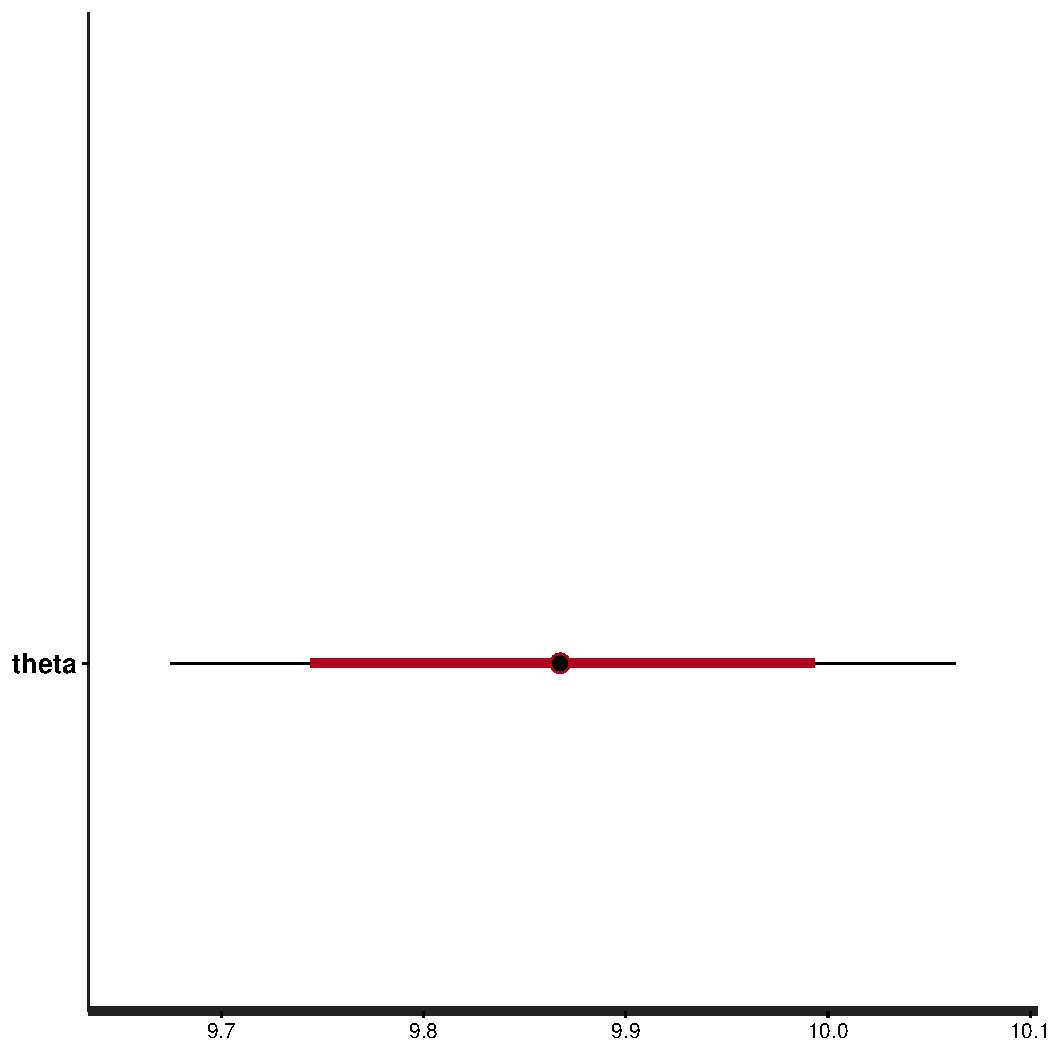
\includegraphics[scale=0.4]{chapter-computing-stan-1}
 \caption{Exemplo de intervalo de credibilidade estimado usando
          o pacote Stan.}
 \label{fig:stan-1}
\end{figure}

\cprotEnv \begin{example}
 \label{ex:ar-k}
 Considere que, dado $\theta$, 
 $X_{i}= \alpha + \sum_{j=1}^{k}{\beta_{j}X_{i-j}} + \epsilon_{i}$,
 onde $\epsilon_{i}$ são i.i.d. e $\epsilon_{i} \sim N(0,1)$.
 Este é um modelo AR(k), 
 uma generalização do modelo que vimos no \cref{ex:ar-1}.
 Considere que $X_{i}=0$ para $1 \leq i \leq k$ e que, a priori,
 $\theta_{i}$ são i.i.d. e $\theta_{i} \sim N(0,1)$.
 Podemos especificar este modelo no stan da seguinte forma:
 \begin{verbatim}
data {
 int<lower=1> k;  //AR(k)
 int<lower=0> n;  //numero de observacoes, minimo=0.
 real y[n];       //vetor de observacoes reais.
}

parameters {
 real alpha;     //media geral.
 real beta[k];   //parametros autoregressivos.
}

model {
 for(ii in (k+1):n) {
  real mu;
  mu <- alpha;
  for(jj in 1:k) {
   mu <- mu + y[ii-jj]*beta[jj];
  }
  y[ii] ~ normal(mu, 1);
 }
}
 \end{verbatim}
 Este modelo pode ser rodado no R usando os seguintes comandos:
\begin{verbatim}
k <- 2
n <- 100
y <- rep(0, n)
alpha <- 10
beta <- c(0.2,0.3)
for(ii in 3:n) y[ii] <- rnorm(1,alpha+sum(y[(ii-k):(ii-1)]*beta[k:1]),1)
amostra <- stan(file="ar-k.stan", 
                data=c("k", "n", "y"), iter=10^4, chains=1)
plot(amostra)
\end{verbatim}
Os intervalos de credibilidade estimados pelo stan
podem ser encontrados na figura \ref{fig:stan-2}.
\begin{figure}
 \centering
 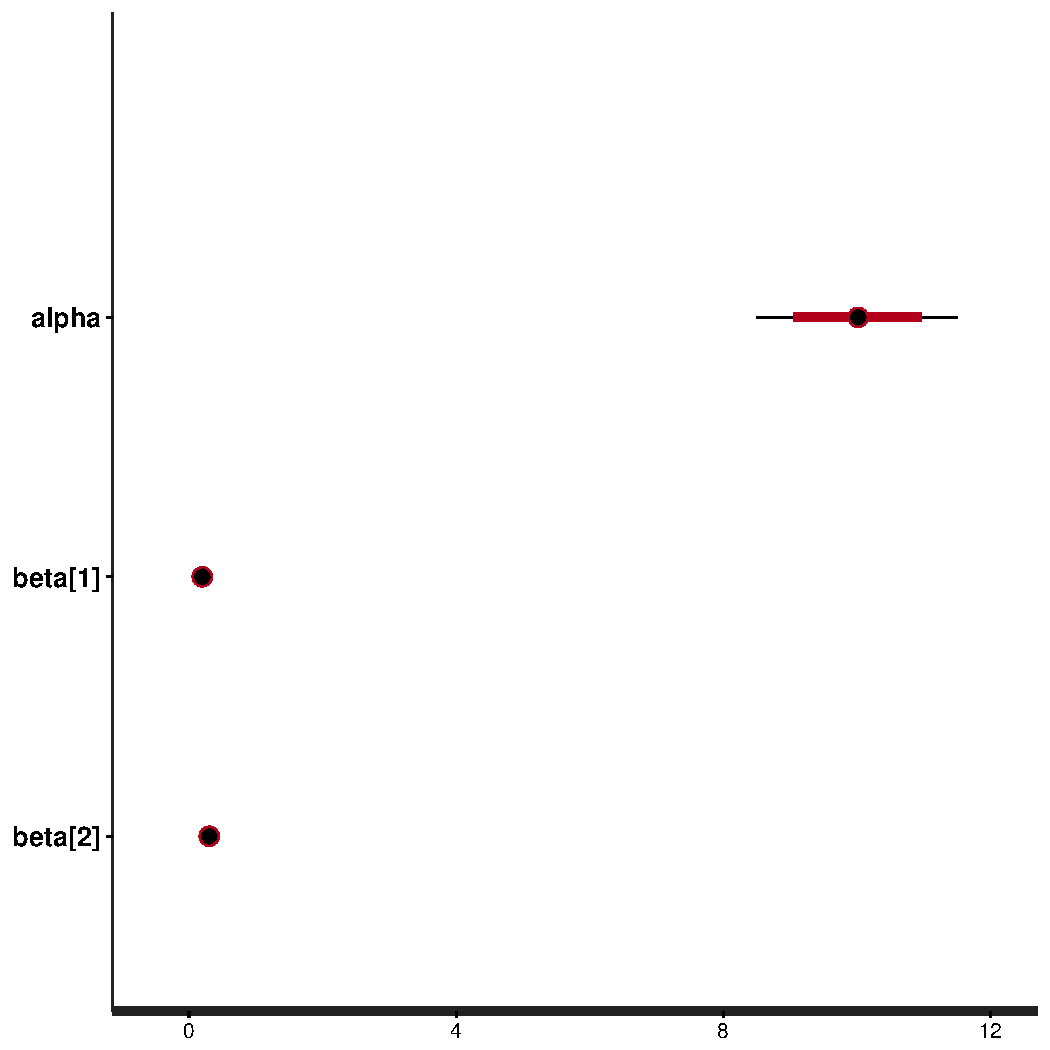
\includegraphics[scale=0.4]{chapter-computing-stan-2}
 \caption{Exemplo de intervalo de credibilidade estimado pelo stan
          para os parâmetros do \cref{ex:ar-k}.}
 \label{fig:stan-2}
\end{figure}
\end{example}

A saída do stan também permite recuperar a Cadeia de Markov.
Por exemplo, no \cref{ex:ar-k}, a Cadeia de Markov para o parâmetro $\alpha$
pode ser recuperada pelo comando
\begin{verbatim}
cadeia <- extract(amostra, "alpha")[["alpha"]]
\end{verbatim}
Podemos usar esta cadeia para estimar a variância de sua média,
assim como no \cref{theorem:clt-markov}.
Para tal, utilizaremos o pacote ``mcmc'' \citep{Geyer2015}.
A variância da média da cadeia é estimada por
\begin{verbatim}
library("mcmc")
olbm(cadeia, 100) //tomamos 100 como 0.01 do tamanho da cadeia.
[1,] 0.0001342983
\end{verbatim}
Podemos também estimar a variância do estimador
para uma função de $\alpha$, como no exemplo $\alpha^{2}$, por
\begin{verbatim}
olbm(cadeia^2, 100)
[1,] 0.05281069
\end{verbatim}

\begin{example}[Regressão linear]

\end{example}

\begin{example}[Regressão linear revisitada]

\end{example}

\begin{example}[Regressão Poisson]

\end{example}

\begin{example}[ANOVA]

\end{example}


Vimos que, usando o pacote ``rstan''
é possível simular Cadeias de Markov que tem
como distribuição estacionária a posteriori.
Este pacote também estima diversas funções da posteriori,
como seus percentis, média e variância.
Também, o pacote ``mcmc'' permite avaliar a
precisão das estimativas acima.
Unindo estes dois pacotes, é possível aplicar a
inferência bayesiana para uma classe ampla de problemas.




\subsubsection{Exercícios}

\begin{exercise}
 \label{ex:anova-stan}
 Considere o \cref{ex:bayesian-anova}.
 \begin{enumerate}[label=(\alph*)]
  \item Gere dados no R considerando que $\mu_{1}=50$, $\mu_{2}=10$, $n=100$ e $\tau_{0}^{2}=1$.
	\item Exiba o código para obter uma Cadeia de Markov para $\mu_{1}$ e $\mu_{2}$ no stan,
	      considerando que $\nu = 20$, $\tau_{1}^{2}=25$ e $\tau_{2}^{2}=10$.
	\item Estime $\mu_{1}$ e $\mu_{2}$ usando a utilidade derivada do erro quadrático.
	\item Construa um intervalo de credibilidade de 95\% para cada parâmetro.
	      Interprete a razão de os intervalos para $\mu_{1}$ e $\mu_{2}$ serem menores 
				do que o intervalo para $\mu$.
	\item Teste a hipótese de M usando a utilidade na tabela \ref{table:u-0-1-c} e $c=1$.
	\item Teste $H_{0}: \mu \geq 20$ usando a utilidade na tabela \ref{table:u-0-1-c} e $c=1$.
 \end{enumerate}
\end{exercise}

\cprotect \solution{\textbf{Solução}:
 \begin{enumerate}[label=(\alph*)]
  \item É possível gerar dados para este problema usando o seguinte código em R:
	\begin{verbatim}
y1 <- rnorm(100,50,1)
y2 <- rnorm(100,10,1)
data <- data.frame(y1,y2)
	\end{verbatim}
	\item É possível obter uma Cadeia de Markov para $\mu_{1}$ e $\mu_{2}$
	      usando o seguinte código em stan.
	\begin{verbatim}
data {
 int<lower=0> N1;   //numero de observacoes para o tratamento 1.
 int<lower=0> N2;   //numero de observacoes para o tratamento 2.
 real y1[N1];       //vetor de observacoes para o tratamento 1.
 real y2[N2];       //vetor de observacoes para o tratamento 2.
}

parameters {
 real mu1;          //contaminacao media sob o tratamento 1.
 real mu2;          //contaminacao media sob o tratamento 2.
 real mu;           //contaminacao media global.
}

model {
 mu ~ normal(20, 10);
 mu1 ~ normal(mu, 25);
 mu2 ~ normal(mu, 25);
 y1 ~ normal(mu1, 1);
 y2 ~ normal(mu2, 1);
}
	\end{verbatim}
	
	\item Utilizando o \cref{thm:estimation_l2},
        sabemos que, sob a utilidade obtida pelo erro quadrático,
				o estimador ótimo é a média a posteriori, 
				ou seja $E[\mu_{1}|y]$ e $E[\mu_{2}|y]$.
				Também, decorre do \cref{theorem:clt-markov} que
				$E[\mu_{i}|y]$ pode ser aproximado pela média
				dos valores obtidos na Cadeia de Markov que
				tem como distribuição estacionária $\pi(\mu_{i}|y)$.
				Portanto, para gerar esta Cadeia de Markov e
				aproximar os valores de $E[\mu_{i}|y]$,
				usamos o seguinte código:
	\begin{verbatim}
amostra <- stan(file="anova.stan", 
                data=c("N1", "N2", "y1", "y2"), iter=10^4, chains=1)	
est_mu1 <- mean(extract(amostra, "mu1")[["mu1"]])
est_mu2 <- mean(extract(amostra, "mu2")[["mu2"]])
c(est_mu1,est_mu2)
[1] 50.12020 10.07273
	\end{verbatim}
  Portanto, $\hat{\mu}_{1} = E[\mu_{1}|y] \approx 50.1$ e 
	$\hat{\mu}_{2} = E[\mu_{2}|y] \approx 10.0$.
	\item Intervalos de credibilidade 95\% podem ser obtidos diretamente pelo comando
	\begin{verbatim}
plot(amostra)
	\end{verbatim}
  \begin{figure}
	 \centering
   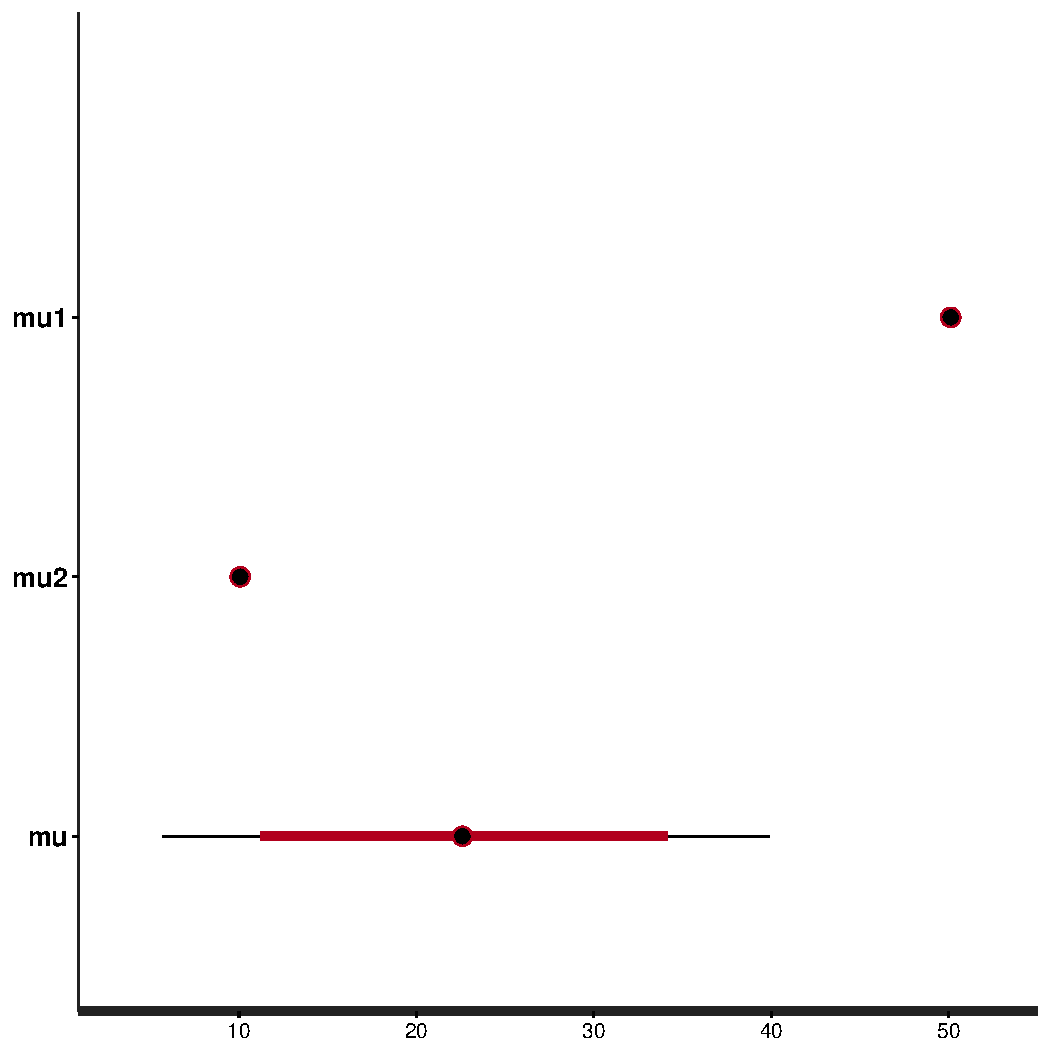
\includegraphics[scale=0.5]{chapter-computing-stan-anova}
	 \caption{Intervalos de credibilidade para $\mu_1$, $\mu_2$ e $\mu$
	          no \cref{ex:anova-stan}.}
	 \label{fig:anova-stan}
	\end{figure}
	O resultado é exibido na figura \ref{fig:anova-stan}.
	Note que os intervalos para $\mu_{1}$ e $\mu_{2}$ são menores
	que o intervalo para $\mu$.
	Para entender este fenômeno, observe que $y_{i,j}|\mu_{i} \sim N(\mu_{i},1)$.
	Também, $\mu_{i}|\mu \sim N(\mu,25)$.
	Em outras palavras, segundo este modelo,
	$y_{i,j}$ trazem informação sobre os $\mu_{i}$ e
	os $\mu_{i}$ trazem informação sobre $\mu$.
	Como há mais valores de $y_{i,j} (200)$ do que de $\mu_{i} (2)$
	e os $y_{i,j}$ tem variância $(1)$ menor que os $\mu_{i} (25)$,
	é razoável esperar que o intervalo de credibilidade para $\mu_{1}$ e $\mu_{2}$
	seja menor que aquele de $\mu$.
	
	\item Desejamos testar $H_{0}: \mu_{1} \leq \mu_{2}$.
	      Decorre do, \cref{thm:0-1-c} que, como $c=1$,
				rejeitamos $H_{0}$ se $P(H_{0}|y) < 0.5$.
				Também, decorre do \cref{theorem:clt-markov} que
				podemos usar uma Cadeia de Markov para aproximar $P(H_{0}|y)$.
				Para tal, podemos construir uma Cadeia $(a_{i},b_{i})$ que 
				tem como distribuição estacionária a 
				posteriori conjunta de $\mu_{1}$ e $\mu_{2}$.
				Sob estas condições, a frequência com que $a_{i} \leq b_{i}$
				aproxima $P(\mu_{1} \leq \mu_{2}|y)$, ou seja $P(H_{0}|y)$.
				Podemos obter esta estimativa usando o seguinte código em R:
\begin{verbatim}
mu1 <- extract(amostra, "mu1")[["mu1"]]
mu2 <- extract(amostra, "mu2")[["mu2"]]
mean(mu1 <= mu2)
[1] 0
\end{verbatim}
	     Assim, obtemos que $P(H_{0}|y) \approx 0$ e rejeitamos $H_{0}$.
			
  \item Similarmente ao item anterior, obtemos:
	\begin{verbatim}
mu <- extract(amostra, "mu")[["mu"]]
mean(mu >= 20)
[1] 0.6086
olbm(mu >= 20, 250)
[1] 4.579868e-05
	\end{verbatim}
	Portanto, como $P(H_{0}|y) \approx 0.6 > 0.5$
	(e olbm indica que o erro de aproximação do
	 Monte Carlo é baixo),
	não rejeitamos $H_{0}$.
 \end{enumerate}
}{}

\begin{exercise}
 Considere o \cref{ex:ad-effect}.
 \begin{enumerate}[label=(\alph*)]
  \item Gere dados no R considerando que $\theta_{1}=100$ e $\theta_{2}=150$ e $n=30$.
	\item Exiba o código para obter uma Cadeia de Markov para $\theta_{1}$ e $\theta_{2}$ no stan, usando $a_1 = a_2 = b_1 = b_2 = 1$.
	\item Construa um intervalo de credibilidade de 95\% para cada parâmetro.
	\item Teste a hipótese de M usando a utilidade na tabela \ref{table:u-0-1-c} e $c=1$.
	\item Como você levaria em conta que o número de acessos pode ser influenciado pelo dia da semana?
	      Sugira um modelo que leve este efeito em consideração e rode-o no stan.
 \end{enumerate}
\end{exercise}

\newpage

\section{Revisão final}

\begin{exercise}
 Considere que $X|\theta \sim \text{Poisson}(\theta)$.
 Um estatístico deseja usar $\pi(\theta) \propto \theta^{-1}$.
 \begin{enumerate}[label=(\alph*)]
  \item A posteriori para $\theta|X=x$ é proporcional a qual função?
	\item Note que a posteriori para $\theta|X=0$ não é integrável e,
	      portanto, não é uma densidade de probabilidade.
				Qual falha permitiu que isso ocorresse?
 \end{enumerate}
\end{exercise}

\bibliographystyle{apalike}
\bibliography{book}

\end{document}
